% Options for packages loaded elsewhere
\PassOptionsToPackage{unicode}{hyperref}
\PassOptionsToPackage{hyphens}{url}
%
\documentclass[
]{article}
\usepackage{lmodern}
\usepackage{amsmath}
\usepackage{ifxetex,ifluatex}
\ifnum 0\ifxetex 1\fi\ifluatex 1\fi=0 % if pdftex
  \usepackage[T1]{fontenc}
  \usepackage[utf8]{inputenc}
  \usepackage{textcomp} % provide euro and other symbols
  \usepackage{amssymb}
\else % if luatex or xetex
  \usepackage{unicode-math}
  \defaultfontfeatures{Scale=MatchLowercase}
  \defaultfontfeatures[\rmfamily]{Ligatures=TeX,Scale=1}
  \setmainfont[]{Times}
\fi
% Use upquote if available, for straight quotes in verbatim environments
\IfFileExists{upquote.sty}{\usepackage{upquote}}{}
\IfFileExists{microtype.sty}{% use microtype if available
  \usepackage[]{microtype}
  \UseMicrotypeSet[protrusion]{basicmath} % disable protrusion for tt fonts
}{}
\makeatletter
\@ifundefined{KOMAClassName}{% if non-KOMA class
  \IfFileExists{parskip.sty}{%
    \usepackage{parskip}
  }{% else
    \setlength{\parindent}{0pt}
    \setlength{\parskip}{6pt plus 2pt minus 1pt}}
}{% if KOMA class
  \KOMAoptions{parskip=half}}
\makeatother
\usepackage{xcolor}
\IfFileExists{xurl.sty}{\usepackage{xurl}}{} % add URL line breaks if available
\IfFileExists{bookmark.sty}{\usepackage{bookmark}}{\usepackage{hyperref}}
\hypersetup{
  pdftitle={Trading social status for genetics in marriage markets: evidence from UK Biobank},
  pdfauthor={David Hugh-Jones, Oana Borcan \& Abdel Abdellaoui},
  hidelinks,
  pdfcreator={LaTeX via pandoc}}
\urlstyle{same} % disable monospaced font for URLs
\usepackage[margin=1in]{geometry}
\usepackage{longtable,booktabs}
\usepackage{calc} % for calculating minipage widths
% Correct order of tables after \paragraph or \subparagraph
\usepackage{etoolbox}
\makeatletter
\patchcmd\longtable{\par}{\if@noskipsec\mbox{}\fi\par}{}{}
\makeatother
% Allow footnotes in longtable head/foot
\IfFileExists{footnotehyper.sty}{\usepackage{footnotehyper}}{\usepackage{footnote}}
\makesavenoteenv{longtable}
\usepackage{graphicx}
\makeatletter
\def\maxwidth{\ifdim\Gin@nat@width>\linewidth\linewidth\else\Gin@nat@width\fi}
\def\maxheight{\ifdim\Gin@nat@height>\textheight\textheight\else\Gin@nat@height\fi}
\makeatother
% Scale images if necessary, so that they will not overflow the page
% margins by default, and it is still possible to overwrite the defaults
% using explicit options in \includegraphics[width, height, ...]{}
\setkeys{Gin}{width=\maxwidth,height=\maxheight,keepaspectratio}
% Set default figure placement to htbp
\makeatletter
\def\fps@figure{htbp}
\makeatother
\setlength{\emergencystretch}{3em} % prevent overfull lines
\providecommand{\tightlist}{%
  \setlength{\itemsep}{0pt}\setlength{\parskip}{0pt}}
\setcounter{secnumdepth}{-\maxdimen} % remove section numbering
\usepackage{subfig}
\usepackage{setspace}\doublespacing
\usepackage{amsmath}
\usepackage{amsthm}
\usepackage{placeins}
\newtheorem{prop}{\protect\propositionname}
\providecommand{\propositionname}{Proposition}
\usepackage{array}
\usepackage{caption}
\usepackage{graphicx}
\usepackage{siunitx}
\usepackage{ulem}
\usepackage{colortbl}
\usepackage{multirow}
\usepackage{hhline}
\usepackage{calc}
\usepackage{tabularx}
\usepackage{threeparttable}
\usepackage{wrapfig}
\usepackage{adjustbox}
\ifluatex
  \usepackage{selnolig}  % disable illegal ligatures
\fi
\newlength{\cslhangindent}
\setlength{\cslhangindent}{1.5em}
\newlength{\csllabelwidth}
\setlength{\csllabelwidth}{3em}
\newenvironment{CSLReferences}[2] % #1 hanging-ident, #2 entry spacing
 {% don't indent paragraphs
  \setlength{\parindent}{0pt}
  % turn on hanging indent if param 1 is 1
  \ifodd #1 \everypar{\setlength{\hangindent}{\cslhangindent}}\ignorespaces\fi
  % set entry spacing
  \ifnum #2 > 0
  \setlength{\parskip}{#2\baselineskip}
  \fi
 }%
 {}
\usepackage{calc}
\newcommand{\CSLBlock}[1]{#1\hfill\break}
\newcommand{\CSLLeftMargin}[1]{\parbox[t]{\csllabelwidth}{#1}}
\newcommand{\CSLRightInline}[1]{\parbox[t]{\linewidth - \csllabelwidth}{#1}\break}
\newcommand{\CSLIndent}[1]{\hspace{\cslhangindent}#1}

\title{Trading social status for genetics in marriage markets: evidence from UK Biobank}
\author{David Hugh-Jones, Oana Borcan \& Abdel Abdellaoui}
\date{2021-03-10}

\begin{document}
\maketitle
\begin{abstract}
Some genetic variants are systematically associated with
socio-economic status. We provide a new explanation for this, based on
marriage markets: if social status and `good genes' are both attractive in
a partner, then they will become associated in the next generation. We test
our theory on couples in UK Biobank, a large genetically-informed survey.
We compare spouses of individuals with different birth order, which is
known to affect socio-economic status and which is
exogenous to own genetic endowments (among siblings). Spouses of
earlier-born siblings have higher polygenic scores for educational
attainment. The effect of birth order appears to be mediated by own
educational attainment. Thus, environmental shocks to social status are
reflected in the DNA of subsequent generations. This mechanism reveals a
new aspect of the inheritance of inequality in contemporary and
historical human societies.
\end{abstract}

\normalem

\hypertarget{introduction}{%
\section{Introduction}\label{introduction}}

Inequality persists over generations, and this has important economic
effects. Intergenerational mobility is correlated with
(within-generation) inequality itself (Krueger 2012; Becker et al. 2018), and it may also affect economic efficiency by
changing the payoffs to talent and hard work (Corak 2013).
Intergenerational absolute mobility has fallen in America
(Chetty et al. 2017), although relative mobility has been stable
(Chetty et al. 2014).

Families play a role in this story, because wealth, human capital and
other traits are transmitted from parents to children. In particular,
assortative mating (when similar people marry each other) can increase
social inequality in income, wealth, social status or human capital,
compared to the case where people pair at random. It is often thought
that the degree of assortative mating has increased in recent
generations, and that this could help to explain increasing levels of
social inequality (Fernandez, Guner, and Knowles 2005; Schwartz and Mare 2005; Greenwood et al. 2014; Eika, Mogstad, and Zafar 2019).

Another strand of research relates inequality to human genetics. Twin
studies show that the heritability of occupational class and educational
attainment, i.e.~the proportion of variance explained by genetic
differences between individuals, is around 50\% (Tambs et al. 1989).
Genome-wide Complex Trait Analysis (GCTA) shows that 2-year-old
children's family socio-economic status (SES) can be predicted from
their genes (Trzaskowski et al. 2014). Polygenic scores for educational
attainment predict occupational class (Rimfeld et al. 2018). The current
leading explanation for this \emph{SES-genetics gradient} is that in
meritocratic societies, individuals with genes associated with valuable
skills and personality traits experience upward mobility. Their children
will then inherit both their genes (via biology) and their increased
social status (via social institutions).

This paper links assortative mating to genetics in order to give a new
explanation for the SES-genetics gradient. The mechanism is that both
social status\footnote{\emph{Social status} refers to characteristics that an individual
  possesses in virtue of their social position. For example, my wealth
  is a fact about me that holds in virtue of my relationship to
  certain social institutions (bank deposits, title deeds et cetera.).
  Other examples include caste, class, income, and educational
  qualifications. \emph{Socio-economic status} (SES) is a specific type of
  social status which exists in economically stratified societies, and
  which refers to a combination of educational attainment,
  occupational class, income and wealth (e.g. White 1982).} and genetics contribute to a person's attractiveness
in marriage markets. For example, suppose that wealth and intelligence
are both attractive qualities in a spouse. Then wealthy people will be
more likely to marry intelligent people. Again, children of these
marriages will then inherit both wealth, and genetic variants associated
with intelligence. As a result, wealth and genes for intelligence will
become associated in the next generation. More generally, whenever
people in marriage markets trade social status for a genetically
inherited characteristic, the two will become associated. We call this
mechanism \emph{Social-Genetic Assortative Mating} (SGAM).

Under this mechanism, shocks to an individual's social status may alter
the identity of his or her spouse, and so be reflected in the genetics
of his or her children. Thus, in contrast to a large body of research
that treats genetic data as an independent variable and traces its
effects on social and economic outcomes, we make the genetics
endogenous.\footnote{Almost all research in behavioural genetics fits this pattern (see
  e.g. Plomin, DeFries, and McClearn 2008). For a review of relevant research in
  economics, see Benjamin et al. (2011). Some more recent economics
  papers use polygenic scores (Barth, Papageorge, and Thom 2020; Papageorge and Thom 2020; Ronda et al. 2020; Sias, Starks, and Turtle 2020).} Our mechanism gives a new explanation for the link
between social status and genetics. This explanation is likely to apply
to a wider range of societies than the alternative ``meritocratic
mobility'' explanation. That is because, while widespread social mobility
is relatively rare and historically recent, assortative mating is a
human universal (Buss 1989).

Below, after reviewing the literature, we develop a simple model of SGAM
to show how parents' social status predicts children's genetics, and how
this varies with a society's marriage market institutions. Surprisingly,
there is a non-linear relationship between ``egalitarianism'' in marriage
markets, and the strength of the association between social status and
genetic variation. When marriage markets are fully egalitarian, or fully
inegalitarian, SGAM does not cause any association. In between these
extremes, there is a positive association. The intuition is that in a
fully ``egalitarian'' marriage market, social status plays no role in
determining attractiveness. As a result, people do not trade off social
status against genetics. On the other hand, in a wholly ``inegalitarian''
marriage market, such as a caste society where mating across castes is
forbidden, only social status determines attractiveness and genetics
plays no role, so again people do not trade the two off. In between the
two extremes, potential spouses trade social status for ``good genes,''
and the two become associated.

We then test for SGAM using contemporary data from the UK. Our dependent
variable is the polygenic score for educational attainment (PSEA) of a
person's spouse. PSEA is a measure, derived solely from an individual's
DNA, predicting the number of years that person will spend in education
(Lee et al. 2018). To detect SGAM, and avoid the potential confound of pure
genetic assortative mating, we use a causal antecedent of social status
which is independent of individual genetics: birth order. Birth order is
known to affect outcomes including income, occupational status and
educational attainment (Black, Devereux, and Salvanes 2005; Booth and Kee 2009). We show that
people born earlier within a sibling group marry spouses with different
genetics, specifically, higher PSEA. We present evidence that this
effect is mediated by measures of socio-economic status, including
educational attainment and labour market income.

\hypertarget{related-literature}{%
\section{Related literature}\label{related-literature}}

There are several ways assortative mating can affect social inequality
(Fernández and Rogerson 2001). The simplest is that if couples assort with
respect to some characteristic, the resulting households will have more
variance in that characteristic than if couples match randomly. For
instance, if rich people only marry each other, then the wealth
distribution of the resulting households will be more unequal than if
they sometimes marry poor people. If the characteristic is inherited
from parents to children, then this will carry over into higher
inter\emph{-individual} inequality in the next generation.

Assortative mating on one dimension can also affect inequality in other
dimensions. For example, if parents invest in their children's human
capital, and if households are credit-constrained, then assortative
mating on income can increase inequality in children's human capital
(Fernandez, Guner, and Knowles 2005). The mechanism is purely environmental, not
genetic: some children are raised in a higher-quality environment (e.g.
with more books and educational toys), and variance in these
environments is increased by assortative mating.

Empirically, it is often thought that assortative mating has increased
since World War II in developed societies, and that this has helped to
increase inequality over time. Several papers test these claims against
US and international data (Fernandez, Guner, and Knowles 2005; Schwartz and Mare 2005; Greenwood et al. 2014; Eika, Mogstad, and Zafar 2019). Overall, there is better
evidence for a rise in assortative mating until the 1980s than
afterwards, and the case that it has contributed to household inequality
is not proven.

Differences in human capital across socio-economic groups also have a
genetic component {[}Tambs et al. (1989); @Trzaskowski\_2014; Rimfeld et al. (2018){]}.
While most human geneticists treat genetic endowments as an independent
variable, there is also research into factors that shape the
distribution of genetic variants. The best-known explanation for the
association between SES and genetics is that in meritocratic societies,
``good genes'' lead to success in education and the labour market.
Successful parents may then pass both SES and their genes to their
children, leading to an association between the two
(Belsky et al. 2018). This mechanism depends on the level of meritocracy
in society's institutions (Heath et al. 1985; Branigan, McCallum, and Freese 2013). In a
wholly non-meritocratic society, where social status was ascribed rather
than earned, this mechanism could not take effect. Indeed, after the
fall of communism in Estonia, the heritability of SES increased,
presumably because post-communist society was more meritocratic
(Rimfeld et al. 2018).

Meritocratic mobility and SGAM are not competing explanations: both may
operate in any specific setting. Both require that SES and genetics are
inherited, which holds to varying degrees in all human societies. While
mobility requires a degree of social openness, so that ``good genes'' can
causally affect a person's social status, SGAM does not need this: even
if social status is inherited from birth, and cannot be earned (as with
e.g.~titles of nobility, or caste), it will still become associated with
attractive genetic variants, so long as there is assortative mating and
people trade status off for genetics in marriage markets. By contrast,
SGAM does require assortative mating (on a combination of SES and
genetics), while meritocratic mobility does not. As a result, SGAM is
likely to apply to a historically wider range of societies. Whilst a
degree of meritocracy exists in modern capitalist economies,
opportunities to earn status have been far more limited in most
societies throughout history (Smelser and Lipset 1966). On the other hand,
assortative mating is likely to be a cultural universal, and SGAM has
probably existed in all societies with inherited status, i.e.~all
societies other than egalitarian hunter-gatherers (Fried 1967).
Thus, SGAM predicts that genetic differences across social status are
likely to be historically ancient.

Another difference is in the chain of causality. In meritocratic
mobility, genetic variants cause an increase in social status, and both
genetics and status may then be inherited. In SGAM, causality may go
from social status to genetics. A shock to one individual's status
causes their spouse to have different genetic variants; again, both
genetics and status are then inherited. As a result, shocks to social
status may be encoded in the genetics of subsequent generations.

Another factor affecting the distribution of genetic endowments is
genetic assortative mating (GAM), the phenomenon that people with
similar genes marry each other. Just as assortative mating can increase
inequality in income or wealth, GAM can increase genetic inequality,
i.e.~the population variance of genetic endowments. Recent research has
confirmed the long-standing conjecture that GAM takes place in
contemporary human populations (Hugh-Jones et al. 2016; Robinson et al. 2017; Howe et al. 2019). Geneticists have also developed
the concept of cross-trait assortative mating (Sundet et al. 2005; Beauchamp et al. 2010), which refers to people with (genes for) e.g.~height
marrying people with (genes for) e.g.~intelligence. As a result, the two
kinds of variation become associated.

To sum up, there are two parallel research traditions on the inheritance
of inequality within families. Each has explored the effects of
assortative mating on different kinds of inequality, and each has
developed theories in which different dimensions of inequality interact.
It seems natural to bring the two literatures together. Here, we do
that, extending the idea of cross-trait assortative mating to encompass
both socially inherited status, and biologically inherited genetic
variants. This leads to a new explanation of the link between
socio-economic status and genetics.

The underlying observations behind SGAM are hardly new. That status and
physical attractiveness tend to assort in marriage markets is a
commonplace, as well as a perennial theme of literature. In the Iliad,
powerful leaders fight over the beautiful slave-girl Bryseis. In Jane
Austen's novels, wealth, attractiveness and ``virtue'' all make a good
match. Marx (1844) wrote ``the effect of ugliness, its repelling
power, is destroyed by money.'' And Donald Trump claimed: ``part of the
beauty of me is that I am very rich.'' There is also a rich literature on
mate preference from evolutionary psychology (Buss 1989; Buss and Barnes 1986; Buss and Schmitt 2019). Attractive mate characteristics
include elements of social status (``high earning capacity,''
``professional status'') as well as traits that are partly under genetic
influence (``intelligent,'' ``tall,'' ``kind,'' ``physically attractive'').

Despite this, surprisingly few papers have analysed the consequences of
SGAM, either within genetics or economics. In economics, several
empirical papers examine cross-trait matching in marriage markets.
Chiappori, Oreffice, and Quintana-Domeque (2012) show empirically that body mass index and SES
(specifically, earnings and education) are both valued in a match.
Oreffice and Quintana-Domeque (2010) show that height and BMI are associated with
spouse earnings. Dupuy and Galichon (2014) find spouse matching on multiple
independent dimensions, including education, height, BMI and
personality; see also Chiappori, Oreffice, and Quintana-Domeque (2018). However, these papers
do not use genetic data, and do not attempt to disentangle genetic and
environmental contributions to attractiveness. They also do not theorize
the consequences of SGAM. Within genetics, Halsey (1958) showed in
a two-class model that social mobility combined with assortative mating
might increase the association between genetics and social class.
Belsky et al. (2018) offer three reasons for the association between
education-linked genetics and SES, but do not consider SGAM.

\hypertarget{model}{%
\section{Model}\label{model}}

There is a large population, whose members have a single genetic trait
\(g_{i}\) and a single social trait \(s_{i}\), drawn from distributions \(G\)
and \(S\). The genetic trait could be, for instance, a polygenic score,
which summarizes the effects of many alleles (genetic variants) at
different loci. The social trait is a measure of social status. Broadly
conceived, this means any trait that an individual possesses in virtue
of his or her position in society, rather than as a natural fact. Caste
and class are kinds of social status; so are wealth, income, education
and employment.

Without loss of generality, \(EG = ES = 0\) and \(Var(G) = Var(S) = 1\).\footnote{Continuous distribution is not strictly required. All that is
  needed is for a set of pairs of positive measure to have different
  values of \(G\) and \(S\), along a set of attractiveness curves of
  positive measure.}
People pair according to an attractiveness function

\[
A(g_{i},s_{i}) = f((1-k)g_{i},ks_{i})
\]

where \(f\) is smooth and strictly increasing in both its arguments, and
\(0 \le k \le 1\). Our sole condition on \(G\) and \(S\) is that a positive
measure of the population has attractiveness \(A\) where the distribution
of \((G, S)|A\) is non-degenerate, i.e.~not everybody with attractiveness
\(A\) is both genetically and socially identical. We assume that people
marry at random within their attractiveness isoquant. One
microfoundation is that \(A\) measures the utility a person provides as a
spouse, and the marriage market works via a Gale-Shapley
(1962) matching mechanism. Or, \(A\) could represent inputs
into a household production function where male and female inputs are
complementary (Becker 1973). Other interpretations are possible:
for instance, different values of \(A\) could represent segmented marriage
markets, like different schools or workplaces.

The key parameter is \(k\). This describes the working of the society's
marriage market. If \(k = 0\), only genetics \(G\) are relevant in marriage
markets, and social status \(S\) has no effect. That is, the marriage
market is highly egalitarian. Conversely, if \(k = 1\), only social status
matters, to the complete exclusion of genetics. This is the equivalent
of a marriage market driven only by ``caste'' or ``class.'' Realistic
societies are between these extremes.

Figure \ref{fig:pic-intuition} shows the intuition behind our theory.
The top row shows a \emph{caste marriage market} with \(k = 1\). A typical pair
is shown: children have intermediate values of \(G\) and \(S\) between their
two parents (hollow circle). In this society pairs match only by social
status; genetics plays no role. As a result, while the variance of \(G\)
shrinks within each status group, genetics remain uncorrelated with
social status in the children's population distribution, shown on the
right. The next row shows a pure \emph{egalitarian marriage market} with
\(k = 0\). Parents match only by genetics and ignore social status. Again,
as a result there is no correlation between genetics and social status
in the children's generation. The bottom row shows a (more realistic)
intermediate society, with an intermediate value of \(k\). Because both
genetics and social status contribute to attractiveness, matched spouses
typically trade them off against each other. As a result, the
distribution is squeezed along the gradient of \(k\), and \(G\) and \(S\) are
correlated in the children's generation. We next prove this formally.

If \(k = 0\), ``indifference curves'' of attractiveness are vertical lines
in \((G, S)\) space. If \(k = 1\), they are horizontal lines. If
\(k \in (0,1)\) they are downward sloping curves.

Write \(p(i)\) for \(i\)'s partner. Pairs always have the same
attractiveness:

\begin{equation}
A(g_{i},s_{i}) = A(g_{p(i)},s_{p(i)}),
\label{eq:same-A}
\end{equation}

Each pair has two children. We assume that both children \(c(d)\) of
parents \(d\), \(m\) have

\begin{align}
g_{c(d)} & =\frac{g_{d}+g_{m}}{2};\label{eq:children-average}\\
s_{c(d)} & =\frac{s_{d}+s_{m}}{2}.\nonumber 
\end{align}

This is a strong simplifying assumption; we relax it below. For real
world examples approximated by the model, \(S\) could be wealth which is
equally divided between the children; \(G\) could be a highly polygenic
trait with many small effects. Write \(G_{p}, S_{p}\) to denote the
population variables in the parents' generation; \(G_{c}, S_{c}\) for the
children's generation.

\begin{prop}
\label{prop:prop1}
(i) $Cov(G_{c}, S_{c}) \ge Cov(G_{p},S_{p})$, with strict inequality
if and only if $0 < k < 1$. 

(ii) If $corr(G_{p}, S_{p}) \ge 0$, then $corr(G_{c},S_{c}) \ge corr(G_{p},S_{p})$,
with strict inequality if and only if $0 < k < 1$ \uline{or} 
$corr(G_{p}, S_{p}) > 0$.
\end{prop}

\begin{figure}

{\centering \subfloat[Caste society ($k = 1$): parents\label{fig:pic-intuition-1}]{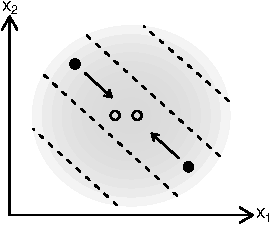
\includegraphics{room-at-the-top_files/figure-latex/pic-intuition-1} }\subfloat[Caste society: children\label{fig:pic-intuition-2}]{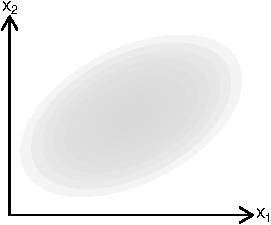
\includegraphics{room-at-the-top_files/figure-latex/pic-intuition-2} }\newline\subfloat[Egalitarian society ($k = 0$): parents\label{fig:pic-intuition-3}]{\includegraphics{room-at-the-top_files/figure-latex/pic-intuition-3} }\subfloat[Egalitarian society: children\label{fig:pic-intuition-4}]{\includegraphics{room-at-the-top_files/figure-latex/pic-intuition-4} }\newline\subfloat[Intermediate society ($0 < k < 1$): parents\label{fig:pic-intuition-5}]{\includegraphics{room-at-the-top_files/figure-latex/pic-intuition-5} }\subfloat[Intermediate society: children\label{fig:pic-intuition-6}]{\includegraphics{room-at-the-top_files/figure-latex/pic-intuition-6} }

}

\caption{Theory: shaded area is the population distribution. Dotted lines are attractiveness isoquants. Solid dots are example parents, transparent dots are example children. The right hand side shows the children's generation.}\label{fig:pic-intuition}
\end{figure}

We view \(k = 0\) and \(k = 1\) as theoretical ``ideal types.'' Proposition
\ref{prop:prop1} therefore shows that in almost any realistic society,
social status will become correlated with genetic traits which are
considered attractive in marriage markets.

We now relax the condition that children are exactly at the mean of
their parents' values for \(G\) and \(S\). Let

\begin{align*}
g_{c(i)} & = \bar{g}_{i}+\varepsilon_{i}^{G} \\
s_{c(i)} & = \bar{s}_{i}+\varepsilon_{i}^{S}
\end{align*}

where

\[
\bar{g}_{i} = \frac{g_{i} + g_{p(i)}}{2}; \bar{s}_{i} = \frac{s_{i} + s_{p(i)}}{2};
\]

\(\varepsilon^{G}\) has mean 0 and variance \(\sigma_{G}^{2}\); and
\(\varepsilon^{S}\) has mean 0 and variance \(\sigma_{S}^{2}\).

\begin{prop}
\label{prop:robustness}

\begin{enumerate}

\item If $\sigma_{G}^{2}$ and $\sigma_{S}^{2}$ are small enough and $corr(G_{p},S_{p}) \ge 0$,
then $corr(G_{c},S_{c}) > corr(G_{p},S_{p})$ for $k \in (0,1)$.

\item If $\varepsilon^{G}$ and $\varepsilon^{S}$ are uncorrelated with
each other and with $\bar{G}$ and $\bar{S}$; and if $G_{p}$ and
$S_{p}$ are uncorrelated, then $corr(G_{c},S_{c}) \ge 0$, with strict
inequality if and only if $0<k<1$.

\end{enumerate}

\end{prop}

The conditions in Proposition \ref{prop:robustness} are quite plausible.
For \(G\), they require that either variance in siblings' scores on some
summary statistic is not too large, or that it is uncorrelated with the
parents' scores. Both of these hold for most polygenic scores, which are
additive sums of many small effects of alleles derived randomly from one
or other parent. For \(S\), the conditions would hold, for example, if \(S\)
measures wealth, which is inherited not too unequally between siblings;
or if wealth is inherited unequally but not in a way that correlates
with \(S\) or \(G\).

It is worth considering what kind of social arrangements would \emph{violate}
these conditions. For example, suppose that parents' combined wealth is
inherited by the child with the lowest value of \(g_{c(i)}\). This creates
a negative correlation between \(s_{c(i)}\) and \(g_{c(i)}\).

In the model, intermediate values of \(k\) drive increased covariance
between genetics and social status. That naturally raises the question
whether the change in covariance and/or correlation is increasing in \(k\)
towards some maximum value in \((0,1)\), then decreasing, i.e., whether it
is quasiconcave in \(k\). In general the answer is no, even on the
assumption that

\begin{equation}
A(g_{i},s_{i}) = (1-k)g_{i} + ks_{i}
\label{eq:linearity}
\end{equation}

i.e.~that indifference curves are straight lines in \((G, S)\) space.
However, quasiconcavity in \(k\) does hold when indifference curves are
straight and \((G, S)\) are jointly normally distributed. We conjecture
that it also holds whenever the distribution \((G, S)\) is log-concave or
even quasiconcave.

\hypertarget{discussion}{%
\subsection{Discussion}\label{discussion}}

The ``marriage market'' here is a reduced form mechanism, encompassing
everything that makes a difference to partner choice. For example, if
earned income affects attractiveness in the marriage market, then
society's level of meritocracy in the labour market will correlate with
the value of \(k\): a more meritocratic labour market will allow people
with low social status but high human capital (genetically determined in
part) to earn more, and therefore to match with more attractive
partners.

The contents of both \(S\), social status, and \(G\) -- ``good genes'' in the
marriage market -- are likely to vary across societies. \(S\) could
encompass variables like social class or caste; ethnic identity in
``ranked'' ethnic systems; or in modern societies, SES. Regarding \(G\),
standards of physical attractiveness, and other characteristics which
make someone a ``good match,'' vary both across societies and within a
society over time.

Recent empirical work shows high persistence of SES over time, in
particular at the top. One suggested reason for this is that unmeasured
family characteristics persist along with measured wealth
(Clark and Cummins 2015). Our model captures this idea. For
simplicity, assume the original model with no noise in children's values
of \(g\) or \(s\) (condition (\eqref{eq:children-average})), and let
condition (\eqref{eq:linearity}) hold. Consider a regression of
children's social status on parent's social status:

\[
s_{c(i)} = \alpha + \beta_S s_i + \varepsilon_{c(i)}.
\]

The value of \(\beta_S\) will be less than one, since parents match on
downward sloping isoattractiveness curves: within each curve, relatively
wealthy individuals match with less wealthy individuals on average. Now
consider a regression of child on parent ``attractiveness'' \(A\):

\[
A_{c(i)} = \alpha + \beta_A A_i + \varepsilon_{c(i)}.
\]

Since children are on the same attractiveness curve as both their
parents, \(\beta_A = 1\). Thus, regressions on measured components of
social status will underestimate true persistence over time, embodied in
genetic variation. Indeed, grandparents' social status will
independently predict grandchildren's social status, even after
controlling for parents' social status, because of the unmeasured
pathway via parents' genetics.

The model predicts variation in the strength of SGAM. In particular, in
``caste societies'' where there is complete endogamy within social status
groups, there is no scope for SGAM, because marriage partners do not
trade off genetics for social status. The model also assumes that social
status is inherited randomly from one parent, in the same way a genetic
allele is inherited. This assumption can be weakened. For example, if
social status is inherited deterministically from the father, then the
results remain unchanged (for each pair of parents, just assume that one
randomly chosen parent is the father).

In modern societies, both SGAM and meritocratic mobility are likely to
be at play. Genetic variants that cause (e.g.) higher income and wealth
will be inherited along with components of social status such as
inherited wealth. At the same time, higher social status and ``good
genes'' will assort in the marriage market, even if that higher social
status is caused by purely environmental variation. Our empirical
analysis shows this latter process at work.

\hypertarget{data-and-methods}{%
\section{Data and methods}\label{data-and-methods}}

To test the theory, we use data from the UK Biobank, a study of about
500,000 individuals born between 1935 and 1970. The Biobank contains
information on respondents' genetics, derived from DNA microarrays,
along with questionnaire data on health and social outcomes.

The Biobank does not contain explicit information on spouse pairs. We
categorize respondents as pairs if they:

\begin{itemize}
\tightlist
\item
  had the same home postcode on at least one occasion;\footnote{Typically a UK postcode contains about 15 properties.}
\item
  both reported the same homeownership/renting status, length of time
  at the address, and number of children;
\item
  attended the same UK Biobank assessment centre on the same day;
\item
  both reported living with their spouse (``husband, wife or partner'');
\item
  consisted of one male and one female.
\end{itemize}

We also eliminate all pairs where either spouse appeared more than once
in the data. This leaves a total of 35682 pairs. Some of
these could be false positives, i.e.~people who are not each others'
spouse but simply live in the same postcode. To validate the accuracy of
our measures, we use genetic relationships. Some respondents in the
Biobank sample have a child who is also in the sample, as inferred from
genetic data. Among our spouse pairs, 511 have a genetic
child of at least one partner in the sample. For 441 of
these, the child is the genetic child of both partners. If this
subsample is representative, then at least
86\% of the pairs who have had a
child, have had a child together. This is a lower bound, because those
who had a child with someone else may also have had a child with the
presumed partner in our data. As a point of comparison, 11\% of families
with dependent children included a stepchild in England and Wales in
2011 (National Statistics 2014).

It is still possible that some pairs in our data may not be actual
spouses. In the appendix, to sign any possible bias in our estimates
resulting from this, we use a dataset of known ``fake pairs.'' We show
that estimated coefficients of interest are closer to zero among these
fake pairs than among our ``real pairs.'' Because of this, any fake pairs
remaining in our data are likely to bias our coefficients towards zero.

Our key dependent variable is spouse's \emph{Polygenic Score for Educational
Attainment} (PSEA). A polygenic score is a DNA-derived summary measure
of genetic risk or propensity for a particular outcome, created from
summing small effects of many common genetic variants, known as Single
Nucleotide Polymorphisms (SNPs). We focus on PSEA, rather than other
polygenic scores, because educational attainment plays a key role in
human mate search. People are attracted to educated potential partners
(Buss and Barnes 1986; Belot and Francesconi 2013); spouse pairs often have
similar levels of educational attainment, as well as similar PSEA
(Vandenberg 1972; Schwartz and Mare 2005; Greenwood et al. 2014; Hugh-Jones et al. 2016). We use per-SNP summary statistics from
(Lee et al. 2018), re-estimated excluding UK Biobank participants, to
calculate PSEA.\footnote{PSEA was computed by summing the alleles across \textasciitilde1.3 million
  genetic variants weighted by their effect sizes as estimated in
  genome-wide association studies (GWASs) that excluded UK Biobank.
  PSEA was then residualized on the first 100 principal components of
  the SNP array data. Further details can be found in
  @abdellaoui2019genetic.} We normalize the score to have mean 0 and variance
1.

PSEA is known to correlate with measures of education, including
university attendance and years of full-time education; from
within-siblings regressions, where PSEA is randomly assigned by the
``lottery of meiosis,'' we know that this correlation is at least partly
causal. We recheck these facts within the UK Biobank sample. In a simple
linear regression (N = 408,524) of university attendance
on PSEA, a one-standard-deviation increase in PSEA was associated with a
9.23\% increase in the probability of
university attendance (p \textless{} 2e-16). In a within-siblings regression
among genetic full siblings (N = 36,748), the
increase was 4.46\% (p \textless{} 2e-16). This
suggests that about half of the raw correlation of PSEA with university
attendance is down to confounds like good environments or parental
nurture, while the remainder is causal.

Figures \ref{fig:pic-basic-corr-uni} and
\ref{fig:pic-basic-corr-income} illustrate the possible consequences of
SGAM. The X axis shows a measure of one partner's socio-economic status:
university attendance (Figure \ref{fig:pic-basic-corr-uni}) or income
(Figure \ref{fig:pic-basic-corr-income}). The Y axis plots the other
partner's mean PSEA. Both males and females who went to university had
spouses with higher PSEA. So did males and females with higher income.
Since DNA is inherited, these people's children will also have higher
PSEA.

\begin{figure}
\subfloat[Female PSEA by male educational attainment\label{fig:pic-basic-corr-uni-1}]{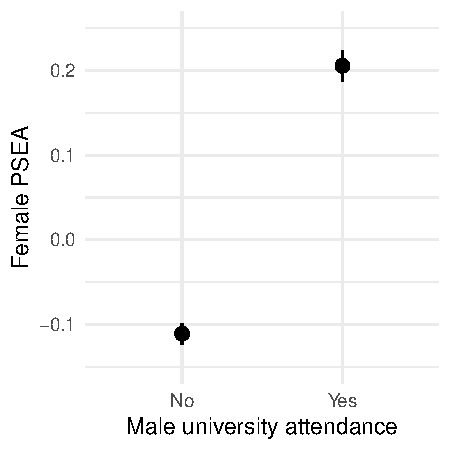
\includegraphics{room-at-the-top_files/figure-latex/pic-basic-corr-uni-1} }\subfloat[Male PSEA by female educational attainment\label{fig:pic-basic-corr-uni-2}]{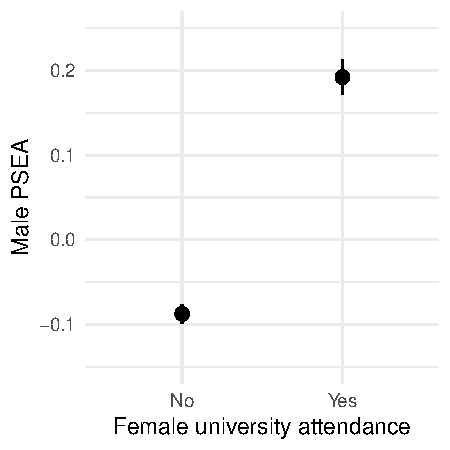
\includegraphics{room-at-the-top_files/figure-latex/pic-basic-corr-uni-2} }\caption{Social and genetic advantage among spouse pairs in UK Biobank}\label{fig:pic-basic-corr-uni}
\end{figure}

\begin{figure}
\subfloat[Female EA3 by male income\label{fig:pic-basic-corr-income-1}]{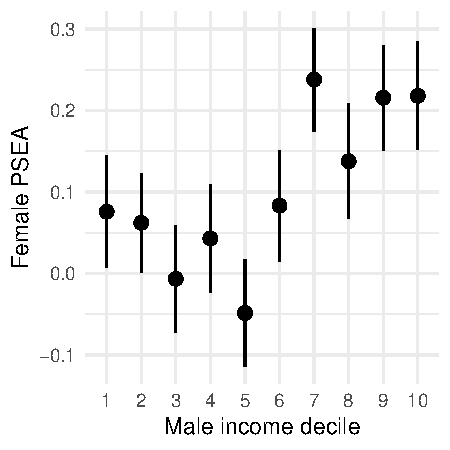
\includegraphics{room-at-the-top_files/figure-latex/pic-basic-corr-income-1} }\subfloat[Male EA3 by female income\label{fig:pic-basic-corr-income-2}]{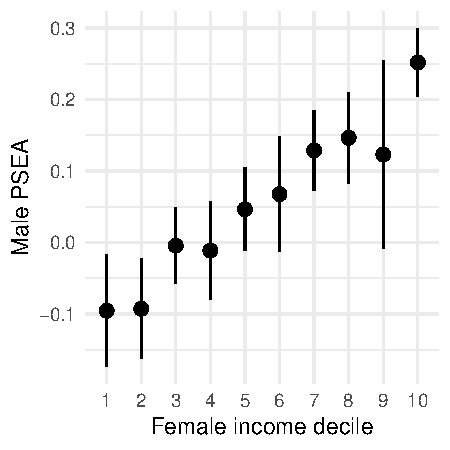
\includegraphics{room-at-the-top_files/figure-latex/pic-basic-corr-income-2} }\caption{Social and genetic advantage among spouse pairs in UK Biobank}\label{fig:pic-basic-corr-income}
\end{figure}

These figures do not prove that SGAM is taking place. Since an
individual's own PSEA correlates with both their educational attainment,
and their income, both figures could be a result of genetic assortative
mating (GAM) alone (Hugh-Jones et al. 2016). To demonstrate SGAM, we need
a source of social status which is exogenous to genetics. Also, the link
between social status and spouse genetics is likely to be noisy, for
three reasons: first, polygenic scores contain a large amount of error;
second, causal mechanisms behind variation in social status are likely
to be noisy; third, to paraphrase Shakespeare (1595), the spouse
matching process is notoriously unpredictable. So, we need a large N to
give us sufficient power. This rules out time-limited shocks such as
changes to the school leaving age (Davies et al. 2018).

We use \emph{birth order}. It is known that earlier-born children receive
more parental care and have better life outcomes, including measures of
SES such as educational attainment and occupational status
(Lindahl 2008; Booth and Kee 2009; Black, Devereux, and Salvanes 2011). On the other hand,
all full siblings have the same \emph{ex ante} expected genetic endowment
from their parents, irrespective of their birth order. For example,
siblings' expected polygenic score is equal to the mean of their
parents' polygenic scores.\footnote{Although genetic variation is randomly assigned to children at
  birth, genetics and birth order could be dependent if parents'
  choice of whether to have more children is endogenous to the genetic
  endowment of their earlier children. We check for this below.} We can therefore use birth order as a
``shock'' to social status. We do not claim that birth order is exogenous
to all other variables. For example, it naturally correlates with
parental age, and it may also relate to the family's economic position
at the time of birth. We only claim that birth order is exogenous to
genetic variation.

Our main independent variable is respondents' birth order, i.e.~their
number of elder siblings plus one. For controls we use family size, i.e.
their total number of siblings including themselves; month of birth; age
at interview; respondents' own PSEA; their father's and/or mother's age
at their birth (calculated from parent's current age, only available if
the parent was still alive). For most regressions, we use only
respondents with between 1 and 5 siblings, i.e.~with a family size of
2-6. To test whether birth order effects are mediated by SES, we use two
measures: income, and university attendance. Current income is a direct
measure of SES, while university attendance is a predictor of income
over the entire life course.

Ideally, we might prefer to use birth order as an instrument for SES.
However, our measures of social status are noisy and incomplete. For
example, we know whether subjects went to university, but not which
university they went to, and we only have rough categorical data on
household income. Birth order likely affects both these measures, and
other, unmeasured dimensions of SES. So, an instrumental variables
approach would probably fall foul of the exclusion restriction.

Instead, we conduct a mediation analysis, following the strategy of
(Heckman, Pinto, and Savelyev 2013). We first confirm statistically that birth
order affects our measures of respondents' SES (income and education).
Then, we regress spouse's PSEA on birth order, with and without
controlling for SES. Under the assumption that birth order is exogenous
to own genetics, these regressions identify the effect of birth order,
plus other environmental variables that correlate with it, on own social
status and spouse's genetics. Also, if the estimated effect of birth
order on spouse's PSEA changes when SES is controlled for, that is
evidence that SES mediates the effect of birth order.

\hypertarget{decomposing-the-birth-order-effect-on-spouse-genetics}{%
\subsection{Decomposing the birth order effect on spouse genetics}\label{decomposing-the-birth-order-effect-on-spouse-genetics}}

Linearizing our model so that \(A(g, s) = (1-k)g + ks\) and applying
\eqref{eq:same-A} shows that:

\[
\frac{d A(g_{p(i)}, s_{p(i)})}{d s_i} = k
\]

We wish to test whether \(k \in (0, 1)\), i.e.~whether SGAM is taking
place. If \(k > 0\) then an increase in \(i\)'s social status \(s_i\) will
increase \(i\)'s attractiveness \(A\); if \(k < 1\) then an increase in \(A\)
will be associated (in expectation) with an increase in \(i\)'s partner's
genetic endowment \(g_{p(i)}\). We therefore wish to estimate the effect
of \(i\)'s status on their partner's genetics, while controlling for \(i\)'s
own genetics \(g_i\). Since our measures of genetic endowment (e.g.~PSEA)
are noisy and incomplete, it is not enough to include them in the
regression. Instead, we use birth order as a source of variation in
\(s_i\) which is orthogonal to \(g_i\).

We follow Heckman, Pinto, and Savelyev (2013) to decompose the aggregate treatment
effect into components due to observed and unobserved proximate channels
affected by the treatment. Our aim is to estimate the effect of SES (as
an effect of birth order) on spouse PSEA.

Assume \(B\) is a variable indicating birth order. The observed outcome
(spouse PSEA) is

\begin{align}
\label{eq:Y}
Y = \sum_{b \in B}Y_b\delta_b
\end{align}

where \(Y_1, Y_2\) etc. are counterfactual outcomes for the first-born,
second-born etc. and \(\delta_b\) is a dummy variable which is 1 if birth
order equals \(b\). Given \(b\), spouse PSEA is assumed to be independent
across observations conditional on some predetermined controls which are
assumed to be unaffected by \(b\).

Let \(\theta_b\) be a set of mediators, i.e.~proximate outcomes determined
by \(b\), which account (at least in part) for the \(b\) treatment effect on
spouse PSEA. We can think of \(\theta_b\) as all the effects on
attractiveness, such as increments to SES, health, cognitive and
non-cognitive skills, that individuals receive due to their birth rank.

Our linear model is

\begin{align}
\label{eq:Yb}
Y_b = \kappa_b + \alpha_b\theta_b + \beta_b \cdot \mathbf{X} + \tilde{\varepsilon}_b
\end{align}

where \(\tilde{\varepsilon}_b\) is a mean-zero residual assumed
independent of \(\theta_b\) and \(\mathbf{X}\). We simplify by assuming that
\(\beta_b = \beta\) and \(\alpha_b = \alpha\) for all \(b\), i.e.~that the
effects of \(\mathbf{X}\) and \(\theta_b\) don't differ by birth order.

We can split the mediators in \(\theta_b\) into a set \(J_m\) of measured
mediators, including measures of SES, and a set \(J_u\) of mediators that
we cannot measure. Write

\begin{align}
\label{eq:Yb2}
Y_b = \tau_b + \sum_{j \in J_m} \alpha^j \theta^j_b + \beta \cdot \mathbf{X} + \varepsilon_b
\end{align}

where \(\tau_b = \kappa_b + \sum_{j \in J_u} \alpha^j E(\theta^j_b)\) and
\(\varepsilon_b = \tilde{\varepsilon}_b + \sum_{j \in J_u} (\theta^j_b - E(\theta^j_b))\).
We assume differences in unmeasured investments due to \(b\) are
independent of \(\mathbf{X}\).

With the assumptions above and substituting \eqref{eq:Yb2} into
\eqref{eq:Y} we obtain:

\begin{align}
\label{eq:Ynew}
Y = \tau_1+\sum_{b \in B\backslash\{1\}} \delta_b(\tau_b-\tau_1) + \sum_{j \in J_m} \alpha^j \theta^j  +   \beta \cdot \mathbf{X} + \varepsilon
\end{align}

where \(\theta^j = \sum_{b \in B}\theta^j_b\delta_b\) and
\(\varepsilon = \sum_{b \in B}\varepsilon_b\delta_b\); \(\tau_b-\tau_1\)
measures the contribution of unmeasured variables to the average
treatment effect of birth order \(b\), relative to birth order 1; and
\(\theta^j, j \in J_m\) denote the observed mediators that we can measure.

Estimating the above by OLS will generate unbiased estimates of
\(\alpha^j\) if \(\theta^j\) is measured without error and is uncorrelated
with the error term \(\varepsilon\). Since \(\varepsilon\) contains both
individual disturbances and differences in unmeasured investments due to
birth order, the identifying assumptions that need to hold for unbiased
OLS estimates are (a) the measured investments (specifically SES) should
be independent of unmeasured investments generated by birth order.
Failing this, the estimates of \(\alpha^j\) will be conflated with the
effects of unmeasured investments. (b) The measured investments should
be uncorrelated with other shocks \(\tilde{\varepsilon}_b\). The overall
treatment effect (relative to birth order \(b = 1\)) can then be
decomposed as follows:

\begin{align}
\label{eq:YbY1}
E(Y_b - Y_1) = \tau_b - \tau_1 + \sum_{j \in J_m} \alpha^j E(\theta^j_b - \theta^j_1)
\end{align}

where \(\tau_b - \tau_1\) is the unmeasured component of the treatment
effect, and \(\sum_{j \in J_m} \alpha^j E(\theta^j_b - \theta^j_1)\) is
the treatment effect due to measured investments.

By running a least square regression of \eqref{eq:YbY1}, we can estimate
\(\tau_b - \tau_1\) . If assumption (a) above holds, the part of the birth
order treatment effect on spouse PSEA that is due to measured mediators,
including SES, can be constructed using the estimated \(\alpha^j\) and the
effects of birth order on measured investments. Specifically, the part
of the birth order effect that is due to university education (or
income) on spouse PSEA will be the coefficient of university (income) in
the regression of spouse PSEA in equation \eqref{eq:Ynew}, multiplied by
the coefficient of birth order from a model where the dependent variable
is an indicator for university (income).

\hypertarget{results}{%
\section{Results}\label{results}}

Figures \ref{fig:pic-bo-uni} and \ref{fig:pic-bo-income} show the
relationship between birth order, university education and income,
separately for respondents with 1-3 siblings. We test this formally in a
linear regression, controlling for family size, which may be correlated
with parental characteristics including genetics. Birth order is
negatively associated with both university attendance and income (among
respondents with 1-5 siblings: university \(p\) = 8.3e-64,
income \(p\) = 6.93e-08).

\begin{figure}
\centering
\includegraphics{room-at-the-top_files/figure-latex/pic-bo-uni-1.pdf}
\caption{\label{fig:pic-bo-uni}University attendance by birth order and family size}
\end{figure}

\begin{figure}
\centering
\includegraphics{room-at-the-top_files/figure-latex/pic-bo-income-1.pdf}
\caption{\label{fig:pic-bo-income}Median income of first job by birth order and family size}
\end{figure}

Next we run regressions of spouse PSEA on birth order, within our
dataset of spouse pairs. Table \ref{tab:tbl-bo-psea-basic} reports the
results. Column 1 controls only for family size (using dummies). As
expected, higher birth order is negatively associated with spouse's
PSEA, though the estimated effect size is small. Column 2 includes the
respondent's own PSEA, as well as dummies for birth year to control for
cohort effects, and dummies for birth month to control for seasonality
effects. The effect size of birth order is not much changed.

Column 3 includes mother's age at birth. Within a family, later children
have older parents by definition. Older parents have more life
experience and may have higher income, which would presumably help later
children.\footnote{There are also potential genetic effects, though\\
  recent research has rejected these in favour of ``social''
  explanations (Kristensen and Bjerkedal 2007; Black, Devereux, and Salvanes 2011).\\
  Cochran and Harpending (2013) report that mutational load is approximately
  linear in father's age, while it is constant in mothers' age. We
  observe very similar results if we control for father's age at
  respondent's birth.} Including mother's age means we can separate the effect
of mother's age from birth order. This reduces the N by a lot, since
only respondents with live mothers reported the necessary data. However,
the effect of birth order jumps in size. Meanwhile, mother's age has a
positive effect. This suggests that the previous estimates mixed two
opposite-signed effects: having older parents versus being later in
birth order.\footnote{Note that parental age would not be a good independent variable
  for testing genetic encoding of social advantage, since it is likely
  to correlate with parents' genetics.}

 
  \providecommand{\huxb}[2]{\arrayrulecolor[RGB]{#1}\global\arrayrulewidth=#2pt}
  \providecommand{\huxvb}[2]{\color[RGB]{#1}\vrule width #2pt}
  \providecommand{\huxtpad}[1]{\rule{0pt}{#1}}
  \providecommand{\huxbpad}[1]{\rule[-#1]{0pt}{#1}}

\begin{table}[ht]
\begin{centerbox}
\begin{threeparttable}
\captionsetup{justification=centering,singlelinecheck=off}
\caption{\label{tab:tbl-bo-psea-basic} Regressions of spouse PSEA on birth order}
 \setlength{\tabcolsep}{0pt}
\begin{tabularx}{0.8\textwidth}{p{0.2\textwidth} p{0.2\textwidth} p{0.2\textwidth} p{0.2\textwidth}}


\hhline{>{\huxb{0, 0, 0}{0.8}}->{\huxb{0, 0, 0}{0.8}}->{\huxb{0, 0, 0}{0.8}}->{\huxb{0, 0, 0}{0.8}}-}
\arrayrulecolor{black}

\multicolumn{1}{!{\huxvb{0, 0, 0}{0}}p{0.2\textwidth}!{\huxvb{0, 0, 0}{0}}}{\hspace{6pt}\parbox[b]{0.2\textwidth-6pt-6pt}{\huxtpad{6pt + 1em}\centering \huxbpad{6pt}}} &
\multicolumn{1}{p{0.2\textwidth}!{\huxvb{0, 0, 0}{0}}}{\hspace{6pt}\parbox[b]{0.2\textwidth-6pt-6pt}{\huxtpad{6pt + 1em}\centering (1)\huxbpad{6pt}}} &
\multicolumn{1}{p{0.2\textwidth}!{\huxvb{0, 0, 0}{0}}}{\hspace{6pt}\parbox[b]{0.2\textwidth-6pt-6pt}{\huxtpad{6pt + 1em}\centering (2)\huxbpad{6pt}}} &
\multicolumn{1}{p{0.2\textwidth}!{\huxvb{0, 0, 0}{0}}}{\hspace{6pt}\parbox[b]{0.2\textwidth-6pt-6pt}{\huxtpad{6pt + 1em}\centering (3)\huxbpad{6pt}}} \tabularnewline[-0.5pt]


\hhline{>{\huxb{255, 255, 255}{0.4}}->{\huxb{0, 0, 0}{0.4}}->{\huxb{0, 0, 0}{0.4}}->{\huxb{0, 0, 0}{0.4}}-}
\arrayrulecolor{black}

\multicolumn{1}{!{\huxvb{0, 0, 0}{0}}p{0.2\textwidth}!{\huxvb{0, 0, 0}{0}}}{\hspace{6pt}\parbox[b]{0.2\textwidth-6pt-6pt}{\huxtpad{6pt + 1em}\raggedright Birth order\huxbpad{6pt}}} &
\multicolumn{1}{p{0.2\textwidth}!{\huxvb{0, 0, 0}{0}}}{\hspace{6pt}\parbox[b]{0.2\textwidth-6pt-6pt}{\huxtpad{6pt + 1em}\raggedleft -0.0084~\huxbpad{6pt}}} &
\multicolumn{1}{p{0.2\textwidth}!{\huxvb{0, 0, 0}{0}}}{\hspace{6pt}\parbox[b]{0.2\textwidth-6pt-6pt}{\huxtpad{6pt + 1em}\raggedleft -0.0066~~~~\huxbpad{6pt}}} &
\multicolumn{1}{p{0.2\textwidth}!{\huxvb{0, 0, 0}{0}}}{\hspace{6pt}\parbox[b]{0.2\textwidth-6pt-6pt}{\huxtpad{6pt + 1em}\raggedleft -0.0325 *~~\huxbpad{6pt}}} \tabularnewline[-0.5pt]


\hhline{}
\arrayrulecolor{black}

\multicolumn{1}{!{\huxvb{0, 0, 0}{0}}p{0.2\textwidth}!{\huxvb{0, 0, 0}{0}}}{\hspace{6pt}\parbox[b]{0.2\textwidth-6pt-6pt}{\huxtpad{6pt + 1em}\raggedright \huxbpad{6pt}}} &
\multicolumn{1}{p{0.2\textwidth}!{\huxvb{0, 0, 0}{0}}}{\hspace{6pt}\parbox[b]{0.2\textwidth-6pt-6pt}{\huxtpad{6pt + 1em}\raggedleft (0.0072)\huxbpad{6pt}}} &
\multicolumn{1}{p{0.2\textwidth}!{\huxvb{0, 0, 0}{0}}}{\hspace{6pt}\parbox[b]{0.2\textwidth-6pt-6pt}{\huxtpad{6pt + 1em}\raggedleft (0.0073)~~~\huxbpad{6pt}}} &
\multicolumn{1}{p{0.2\textwidth}!{\huxvb{0, 0, 0}{0}}}{\hspace{6pt}\parbox[b]{0.2\textwidth-6pt-6pt}{\huxtpad{6pt + 1em}\raggedleft (0.0158)~~~\huxbpad{6pt}}} \tabularnewline[-0.5pt]


\hhline{}
\arrayrulecolor{black}

\multicolumn{1}{!{\huxvb{0, 0, 0}{0}}p{0.2\textwidth}!{\huxvb{0, 0, 0}{0}}}{\hspace{6pt}\parbox[b]{0.2\textwidth-6pt-6pt}{\huxtpad{6pt + 1em}\raggedright Own PSEA\huxbpad{6pt}}} &
\multicolumn{1}{p{0.2\textwidth}!{\huxvb{0, 0, 0}{0}}}{\hspace{6pt}\parbox[b]{0.2\textwidth-6pt-6pt}{\huxtpad{6pt + 1em}\raggedleft ~~~~~~\huxbpad{6pt}}} &
\multicolumn{1}{p{0.2\textwidth}!{\huxvb{0, 0, 0}{0}}}{\hspace{6pt}\parbox[b]{0.2\textwidth-6pt-6pt}{\huxtpad{6pt + 1em}\raggedleft 0.0655 ***\huxbpad{6pt}}} &
\multicolumn{1}{p{0.2\textwidth}!{\huxvb{0, 0, 0}{0}}}{\hspace{6pt}\parbox[b]{0.2\textwidth-6pt-6pt}{\huxtpad{6pt + 1em}\raggedleft 0.0604 ***\huxbpad{6pt}}} \tabularnewline[-0.5pt]


\hhline{}
\arrayrulecolor{black}

\multicolumn{1}{!{\huxvb{0, 0, 0}{0}}p{0.2\textwidth}!{\huxvb{0, 0, 0}{0}}}{\hspace{6pt}\parbox[b]{0.2\textwidth-6pt-6pt}{\huxtpad{6pt + 1em}\raggedright \huxbpad{6pt}}} &
\multicolumn{1}{p{0.2\textwidth}!{\huxvb{0, 0, 0}{0}}}{\hspace{6pt}\parbox[b]{0.2\textwidth-6pt-6pt}{\huxtpad{6pt + 1em}\raggedleft ~~~~~~\huxbpad{6pt}}} &
\multicolumn{1}{p{0.2\textwidth}!{\huxvb{0, 0, 0}{0}}}{\hspace{6pt}\parbox[b]{0.2\textwidth-6pt-6pt}{\huxtpad{6pt + 1em}\raggedleft (0.0064)~~~\huxbpad{6pt}}} &
\multicolumn{1}{p{0.2\textwidth}!{\huxvb{0, 0, 0}{0}}}{\hspace{6pt}\parbox[b]{0.2\textwidth-6pt-6pt}{\huxtpad{6pt + 1em}\raggedleft (0.0107)~~~\huxbpad{6pt}}} \tabularnewline[-0.5pt]


\hhline{}
\arrayrulecolor{black}

\multicolumn{1}{!{\huxvb{0, 0, 0}{0}}p{0.2\textwidth}!{\huxvb{0, 0, 0}{0}}}{\hspace{6pt}\parbox[b]{0.2\textwidth-6pt-6pt}{\huxtpad{6pt + 1em}\raggedright Mother's age at birth\huxbpad{6pt}}} &
\multicolumn{1}{p{0.2\textwidth}!{\huxvb{0, 0, 0}{0}}}{\hspace{6pt}\parbox[b]{0.2\textwidth-6pt-6pt}{\huxtpad{6pt + 1em}\raggedleft ~~~~~~\huxbpad{6pt}}} &
\multicolumn{1}{p{0.2\textwidth}!{\huxvb{0, 0, 0}{0}}}{\hspace{6pt}\parbox[b]{0.2\textwidth-6pt-6pt}{\huxtpad{6pt + 1em}\raggedleft ~~~~~~~~~\huxbpad{6pt}}} &
\multicolumn{1}{p{0.2\textwidth}!{\huxvb{0, 0, 0}{0}}}{\hspace{6pt}\parbox[b]{0.2\textwidth-6pt-6pt}{\huxtpad{6pt + 1em}\raggedleft 0.0102 ***\huxbpad{6pt}}} \tabularnewline[-0.5pt]


\hhline{}
\arrayrulecolor{black}

\multicolumn{1}{!{\huxvb{0, 0, 0}{0}}p{0.2\textwidth}!{\huxvb{0, 0, 0}{0}}}{\hspace{6pt}\parbox[b]{0.2\textwidth-6pt-6pt}{\huxtpad{6pt + 1em}\raggedright \huxbpad{6pt}}} &
\multicolumn{1}{p{0.2\textwidth}!{\huxvb{0, 0, 0}{0}}}{\hspace{6pt}\parbox[b]{0.2\textwidth-6pt-6pt}{\huxtpad{6pt + 1em}\raggedleft ~~~~~~\huxbpad{6pt}}} &
\multicolumn{1}{p{0.2\textwidth}!{\huxvb{0, 0, 0}{0}}}{\hspace{6pt}\parbox[b]{0.2\textwidth-6pt-6pt}{\huxtpad{6pt + 1em}\raggedleft ~~~~~~~~~\huxbpad{6pt}}} &
\multicolumn{1}{p{0.2\textwidth}!{\huxvb{0, 0, 0}{0}}}{\hspace{6pt}\parbox[b]{0.2\textwidth-6pt-6pt}{\huxtpad{6pt + 1em}\raggedleft (0.0028)~~~\huxbpad{6pt}}} \tabularnewline[-0.5pt]


\hhline{>{\huxb{255, 255, 255}{0.4}}->{\huxb{0, 0, 0}{0.4}}->{\huxb{0, 0, 0}{0.4}}->{\huxb{0, 0, 0}{0.4}}-}
\arrayrulecolor{black}

\multicolumn{1}{!{\huxvb{0, 0, 0}{0}}p{0.2\textwidth}!{\huxvb{0, 0, 0}{0}}}{\hspace{6pt}\parbox[b]{0.2\textwidth-6pt-6pt}{\huxtpad{6pt + 1em}\raggedright Family size dummies\huxbpad{6pt}}} &
\multicolumn{1}{p{0.2\textwidth}!{\huxvb{0, 0, 0}{0}}}{\hspace{6pt}\parbox[b]{0.2\textwidth-6pt-6pt}{\huxtpad{6pt + 1em}\raggedleft Yes~~~~~~\huxbpad{6pt}}} &
\multicolumn{1}{p{0.2\textwidth}!{\huxvb{0, 0, 0}{0}}}{\hspace{6pt}\parbox[b]{0.2\textwidth-6pt-6pt}{\huxtpad{6pt + 1em}\raggedleft Yes~~~~~~~~~\huxbpad{6pt}}} &
\multicolumn{1}{p{0.2\textwidth}!{\huxvb{0, 0, 0}{0}}}{\hspace{6pt}\parbox[b]{0.2\textwidth-6pt-6pt}{\huxtpad{6pt + 1em}\raggedleft Yes~~~~~~~~~\huxbpad{6pt}}} \tabularnewline[-0.5pt]


\hhline{}
\arrayrulecolor{black}

\multicolumn{1}{!{\huxvb{0, 0, 0}{0}}p{0.2\textwidth}!{\huxvb{0, 0, 0}{0}}}{\hspace{6pt}\parbox[b]{0.2\textwidth-6pt-6pt}{\huxtpad{6pt + 1em}\raggedright Birth month dummies\huxbpad{6pt}}} &
\multicolumn{1}{p{0.2\textwidth}!{\huxvb{0, 0, 0}{0}}}{\hspace{6pt}\parbox[b]{0.2\textwidth-6pt-6pt}{\huxtpad{6pt + 1em}\raggedleft No~~~~~~\huxbpad{6pt}}} &
\multicolumn{1}{p{0.2\textwidth}!{\huxvb{0, 0, 0}{0}}}{\hspace{6pt}\parbox[b]{0.2\textwidth-6pt-6pt}{\huxtpad{6pt + 1em}\raggedleft Yes~~~~~~~~~\huxbpad{6pt}}} &
\multicolumn{1}{p{0.2\textwidth}!{\huxvb{0, 0, 0}{0}}}{\hspace{6pt}\parbox[b]{0.2\textwidth-6pt-6pt}{\huxtpad{6pt + 1em}\raggedleft Yes~~~~~~~~~\huxbpad{6pt}}} \tabularnewline[-0.5pt]


\hhline{}
\arrayrulecolor{black}

\multicolumn{1}{!{\huxvb{0, 0, 0}{0}}p{0.2\textwidth}!{\huxvb{0, 0, 0}{0}}}{\hspace{6pt}\parbox[b]{0.2\textwidth-6pt-6pt}{\huxtpad{6pt + 1em}\raggedright Birth year dummies\huxbpad{6pt}}} &
\multicolumn{1}{p{0.2\textwidth}!{\huxvb{0, 0, 0}{0}}}{\hspace{6pt}\parbox[b]{0.2\textwidth-6pt-6pt}{\huxtpad{6pt + 1em}\raggedleft No~~~~~~\huxbpad{6pt}}} &
\multicolumn{1}{p{0.2\textwidth}!{\huxvb{0, 0, 0}{0}}}{\hspace{6pt}\parbox[b]{0.2\textwidth-6pt-6pt}{\huxtpad{6pt + 1em}\raggedleft Yes~~~~~~~~~\huxbpad{6pt}}} &
\multicolumn{1}{p{0.2\textwidth}!{\huxvb{0, 0, 0}{0}}}{\hspace{6pt}\parbox[b]{0.2\textwidth-6pt-6pt}{\huxtpad{6pt + 1em}\raggedleft Yes~~~~~~~~~\huxbpad{6pt}}} \tabularnewline[-0.5pt]


\hhline{>{\huxb{255, 255, 255}{0.4}}->{\huxb{0, 0, 0}{0.4}}->{\huxb{0, 0, 0}{0.4}}->{\huxb{0, 0, 0}{0.4}}-}
\arrayrulecolor{black}

\multicolumn{1}{!{\huxvb{0, 0, 0}{0}}p{0.2\textwidth}!{\huxvb{0, 0, 0}{0}}}{\hspace{6pt}\parbox[b]{0.2\textwidth-6pt-6pt}{\huxtpad{6pt + 1em}\raggedright N\huxbpad{6pt}}} &
\multicolumn{1}{p{0.2\textwidth}!{\huxvb{0, 0, 0}{0}}}{\hspace{6pt}\parbox[b]{0.2\textwidth-6pt-6pt}{\huxtpad{6pt + 1em}\raggedleft 24624~~~~~~\huxbpad{6pt}}} &
\multicolumn{1}{p{0.2\textwidth}!{\huxvb{0, 0, 0}{0}}}{\hspace{6pt}\parbox[b]{0.2\textwidth-6pt-6pt}{\huxtpad{6pt + 1em}\raggedleft 24580~~~~~~~~~\huxbpad{6pt}}} &
\multicolumn{1}{p{0.2\textwidth}!{\huxvb{0, 0, 0}{0}}}{\hspace{6pt}\parbox[b]{0.2\textwidth-6pt-6pt}{\huxtpad{6pt + 1em}\raggedleft 8970~~~~~~~~~\huxbpad{6pt}}} \tabularnewline[-0.5pt]


\hhline{}
\arrayrulecolor{black}

\multicolumn{1}{!{\huxvb{0, 0, 0}{0}}p{0.2\textwidth}!{\huxvb{0, 0, 0}{0}}}{\hspace{6pt}\parbox[b]{0.2\textwidth-6pt-6pt}{\huxtpad{6pt + 1em}\raggedright R2\huxbpad{6pt}}} &
\multicolumn{1}{p{0.2\textwidth}!{\huxvb{0, 0, 0}{0}}}{\hspace{6pt}\parbox[b]{0.2\textwidth-6pt-6pt}{\huxtpad{6pt + 1em}\raggedleft 0.003~~\huxbpad{6pt}}} &
\multicolumn{1}{p{0.2\textwidth}!{\huxvb{0, 0, 0}{0}}}{\hspace{6pt}\parbox[b]{0.2\textwidth-6pt-6pt}{\huxtpad{6pt + 1em}\raggedleft 0.010~~~~~\huxbpad{6pt}}} &
\multicolumn{1}{p{0.2\textwidth}!{\huxvb{0, 0, 0}{0}}}{\hspace{6pt}\parbox[b]{0.2\textwidth-6pt-6pt}{\huxtpad{6pt + 1em}\raggedleft 0.013~~~~~\huxbpad{6pt}}} \tabularnewline[-0.5pt]


\hhline{>{\huxb{0, 0, 0}{0.8}}->{\huxb{0, 0, 0}{0.8}}->{\huxb{0, 0, 0}{0.8}}->{\huxb{0, 0, 0}{0.8}}-}
\arrayrulecolor{black}

\multicolumn{4}{!{\huxvb{0, 0, 0}{0}}p{0.8\textwidth+6\tabcolsep}!{\huxvb{0, 0, 0}{0}}}{\hspace{6pt}\parbox[b]{0.8\textwidth+6\tabcolsep-6pt-6pt}{\huxtpad{6pt + 1em}\raggedright  *** p $<$ 0.001;  ** p $<$ 0.01;  * p $<$ 0.05;  + p $<$ 0.1. Standard errors: robust.\huxbpad{6pt}}} \tabularnewline[-0.5pt]


\hhline{}
\arrayrulecolor{black}
\end{tabularx}
\end{threeparttable}\par\end{centerbox}

\end{table}
 

Having tested that birth order affects spouse's PSEA, we now look for
potential mediators of this effect. Despite the lower N, we continue to
control for respondents' fathers' age, since this removes a confound
which would bias our results towards zero.\footnote{The appendix reports results without controlling for father's age.}

 
  \providecommand{\huxb}[2]{\arrayrulecolor[RGB]{#1}\global\arrayrulewidth=#2pt}
  \providecommand{\huxvb}[2]{\color[RGB]{#1}\vrule width #2pt}
  \providecommand{\huxtpad}[1]{\rule{0pt}{#1}}
  \providecommand{\huxbpad}[1]{\rule[-#1]{0pt}{#1}}

\begin{table}[ht]
\begin{centerbox}
\begin{threeparttable}
\captionsetup{justification=centering,singlelinecheck=off}
\caption{\label{tab:tbl-bo-psea} Regressions of spouse PSEA on birth order and potential mediators}
 \setlength{\tabcolsep}{0pt}
\begin{tabular}{l l l l l l}


\hhline{>{\huxb{0, 0, 0}{0.8}}->{\huxb{0, 0, 0}{0.8}}->{\huxb{0, 0, 0}{0.8}}->{\huxb{0, 0, 0}{0.8}}->{\huxb{0, 0, 0}{0.8}}->{\huxb{0, 0, 0}{0.8}}-}
\arrayrulecolor{black}

\multicolumn{1}{!{\huxvb{0, 0, 0}{0}}c!{\huxvb{0, 0, 0}{0}}}{\huxtpad{6pt + 1em}\centering \hspace{6pt}  \hspace{6pt}\huxbpad{6pt}} &
\multicolumn{1}{c!{\huxvb{0, 0, 0}{0}}}{\huxtpad{6pt + 1em}\centering \hspace{6pt} (1) \hspace{6pt}\huxbpad{6pt}} &
\multicolumn{1}{c!{\huxvb{0, 0, 0}{0}}}{\huxtpad{6pt + 1em}\centering \hspace{6pt} (2) \hspace{6pt}\huxbpad{6pt}} &
\multicolumn{1}{c!{\huxvb{0, 0, 0}{0}}}{\huxtpad{6pt + 1em}\centering \hspace{6pt} (3) \hspace{6pt}\huxbpad{6pt}} &
\multicolumn{1}{c!{\huxvb{0, 0, 0}{0}}}{\huxtpad{6pt + 1em}\centering \hspace{6pt} (4) \hspace{6pt}\huxbpad{6pt}} &
\multicolumn{1}{c!{\huxvb{0, 0, 0}{0}}}{\huxtpad{6pt + 1em}\centering \hspace{6pt} (5) \hspace{6pt}\huxbpad{6pt}} \tabularnewline[-0.5pt]


\hhline{>{\huxb{255, 255, 255}{0.4}}->{\huxb{0, 0, 0}{0.4}}->{\huxb{0, 0, 0}{0.4}}->{\huxb{0, 0, 0}{0.4}}->{\huxb{0, 0, 0}{0.4}}->{\huxb{0, 0, 0}{0.4}}-}
\arrayrulecolor{black}

\multicolumn{1}{!{\huxvb{0, 0, 0}{0}}l!{\huxvb{0, 0, 0}{0}}}{\huxtpad{6pt + 1em}\raggedright \hspace{6pt} Birth order \hspace{6pt}\huxbpad{6pt}} &
\multicolumn{1}{r!{\huxvb{0, 0, 0}{0}}}{\huxtpad{6pt + 1em}\raggedleft \hspace{6pt} -0.0325 *~~ \hspace{6pt}\huxbpad{6pt}} &
\multicolumn{1}{r!{\huxvb{0, 0, 0}{0}}}{\huxtpad{6pt + 1em}\raggedleft \hspace{6pt} -0.0173~~~~ \hspace{6pt}\huxbpad{6pt}} &
\multicolumn{1}{r!{\huxvb{0, 0, 0}{0}}}{\huxtpad{6pt + 1em}\raggedleft \hspace{6pt} -0.0040~~~~ \hspace{6pt}\huxbpad{6pt}} &
\multicolumn{1}{r!{\huxvb{0, 0, 0}{0}}}{\huxtpad{6pt + 1em}\raggedleft \hspace{6pt} 0.0094~~~ \hspace{6pt}\huxbpad{6pt}} &
\multicolumn{1}{r!{\huxvb{0, 0, 0}{0}}}{\huxtpad{6pt + 1em}\raggedleft \hspace{6pt} 0.0158~~~~ \hspace{6pt}\huxbpad{6pt}} \tabularnewline[-0.5pt]


\hhline{}
\arrayrulecolor{black}

\multicolumn{1}{!{\huxvb{0, 0, 0}{0}}l!{\huxvb{0, 0, 0}{0}}}{\huxtpad{6pt + 1em}\raggedright \hspace{6pt}  \hspace{6pt}\huxbpad{6pt}} &
\multicolumn{1}{r!{\huxvb{0, 0, 0}{0}}}{\huxtpad{6pt + 1em}\raggedleft \hspace{6pt} (0.0158)~~~ \hspace{6pt}\huxbpad{6pt}} &
\multicolumn{1}{r!{\huxvb{0, 0, 0}{0}}}{\huxtpad{6pt + 1em}\raggedleft \hspace{6pt} (0.0160)~~~ \hspace{6pt}\huxbpad{6pt}} &
\multicolumn{1}{r!{\huxvb{0, 0, 0}{0}}}{\huxtpad{6pt + 1em}\raggedleft \hspace{6pt} (0.0160)~~~ \hspace{6pt}\huxbpad{6pt}} &
\multicolumn{1}{r!{\huxvb{0, 0, 0}{0}}}{\huxtpad{6pt + 1em}\raggedleft \hspace{6pt} (0.0296)~~ \hspace{6pt}\huxbpad{6pt}} &
\multicolumn{1}{r!{\huxvb{0, 0, 0}{0}}}{\huxtpad{6pt + 1em}\raggedleft \hspace{6pt} (0.0296)~~~ \hspace{6pt}\huxbpad{6pt}} \tabularnewline[-0.5pt]


\hhline{}
\arrayrulecolor{black}

\multicolumn{1}{!{\huxvb{0, 0, 0}{0}}l!{\huxvb{0, 0, 0}{0}}}{\huxtpad{6pt + 1em}\raggedright \hspace{6pt} University \hspace{6pt}\huxbpad{6pt}} &
\multicolumn{1}{r!{\huxvb{0, 0, 0}{0}}}{\huxtpad{6pt + 1em}\raggedleft \hspace{6pt} ~~~~~~~~~ \hspace{6pt}\huxbpad{6pt}} &
\multicolumn{1}{r!{\huxvb{0, 0, 0}{0}}}{\huxtpad{6pt + 1em}\raggedleft \hspace{6pt} ~~~~~~~~~ \hspace{6pt}\huxbpad{6pt}} &
\multicolumn{1}{r!{\huxvb{0, 0, 0}{0}}}{\huxtpad{6pt + 1em}\raggedleft \hspace{6pt} 0.2282 *** \hspace{6pt}\huxbpad{6pt}} &
\multicolumn{1}{r!{\huxvb{0, 0, 0}{0}}}{\huxtpad{6pt + 1em}\raggedleft \hspace{6pt} ~~~~~~~~ \hspace{6pt}\huxbpad{6pt}} &
\multicolumn{1}{r!{\huxvb{0, 0, 0}{0}}}{\huxtpad{6pt + 1em}\raggedleft \hspace{6pt} 0.1417 *** \hspace{6pt}\huxbpad{6pt}} \tabularnewline[-0.5pt]


\hhline{}
\arrayrulecolor{black}

\multicolumn{1}{!{\huxvb{0, 0, 0}{0}}l!{\huxvb{0, 0, 0}{0}}}{\huxtpad{6pt + 1em}\raggedright \hspace{6pt}  \hspace{6pt}\huxbpad{6pt}} &
\multicolumn{1}{r!{\huxvb{0, 0, 0}{0}}}{\huxtpad{6pt + 1em}\raggedleft \hspace{6pt} ~~~~~~~~~ \hspace{6pt}\huxbpad{6pt}} &
\multicolumn{1}{r!{\huxvb{0, 0, 0}{0}}}{\huxtpad{6pt + 1em}\raggedleft \hspace{6pt} ~~~~~~~~~ \hspace{6pt}\huxbpad{6pt}} &
\multicolumn{1}{r!{\huxvb{0, 0, 0}{0}}}{\huxtpad{6pt + 1em}\raggedleft \hspace{6pt} (0.0242)~~~ \hspace{6pt}\huxbpad{6pt}} &
\multicolumn{1}{r!{\huxvb{0, 0, 0}{0}}}{\huxtpad{6pt + 1em}\raggedleft \hspace{6pt} ~~~~~~~~ \hspace{6pt}\huxbpad{6pt}} &
\multicolumn{1}{r!{\huxvb{0, 0, 0}{0}}}{\huxtpad{6pt + 1em}\raggedleft \hspace{6pt} (0.0408)~~~ \hspace{6pt}\huxbpad{6pt}} \tabularnewline[-0.5pt]


\hhline{}
\arrayrulecolor{black}

\multicolumn{1}{!{\huxvb{0, 0, 0}{0}}l!{\huxvb{0, 0, 0}{0}}}{\huxtpad{6pt + 1em}\raggedright \hspace{6pt} Income \hspace{6pt}\huxbpad{6pt}} &
\multicolumn{1}{r!{\huxvb{0, 0, 0}{0}}}{\huxtpad{6pt + 1em}\raggedleft \hspace{6pt} ~~~~~~~~~ \hspace{6pt}\huxbpad{6pt}} &
\multicolumn{1}{r!{\huxvb{0, 0, 0}{0}}}{\huxtpad{6pt + 1em}\raggedleft \hspace{6pt} ~~~~~~~~~ \hspace{6pt}\huxbpad{6pt}} &
\multicolumn{1}{r!{\huxvb{0, 0, 0}{0}}}{\huxtpad{6pt + 1em}\raggedleft \hspace{6pt} ~~~~~~~~~ \hspace{6pt}\huxbpad{6pt}} &
\multicolumn{1}{r!{\huxvb{0, 0, 0}{0}}}{\huxtpad{6pt + 1em}\raggedleft \hspace{6pt} 0.0034 ** \hspace{6pt}\huxbpad{6pt}} &
\multicolumn{1}{r!{\huxvb{0, 0, 0}{0}}}{\huxtpad{6pt + 1em}\raggedleft \hspace{6pt} 0.0027 *~~ \hspace{6pt}\huxbpad{6pt}} \tabularnewline[-0.5pt]


\hhline{}
\arrayrulecolor{black}

\multicolumn{1}{!{\huxvb{0, 0, 0}{0}}l!{\huxvb{0, 0, 0}{0}}}{\huxtpad{6pt + 1em}\raggedright \hspace{6pt}  \hspace{6pt}\huxbpad{6pt}} &
\multicolumn{1}{r!{\huxvb{0, 0, 0}{0}}}{\huxtpad{6pt + 1em}\raggedleft \hspace{6pt} ~~~~~~~~~ \hspace{6pt}\huxbpad{6pt}} &
\multicolumn{1}{r!{\huxvb{0, 0, 0}{0}}}{\huxtpad{6pt + 1em}\raggedleft \hspace{6pt} ~~~~~~~~~ \hspace{6pt}\huxbpad{6pt}} &
\multicolumn{1}{r!{\huxvb{0, 0, 0}{0}}}{\huxtpad{6pt + 1em}\raggedleft \hspace{6pt} ~~~~~~~~~ \hspace{6pt}\huxbpad{6pt}} &
\multicolumn{1}{r!{\huxvb{0, 0, 0}{0}}}{\huxtpad{6pt + 1em}\raggedleft \hspace{6pt} (0.0012)~~ \hspace{6pt}\huxbpad{6pt}} &
\multicolumn{1}{r!{\huxvb{0, 0, 0}{0}}}{\huxtpad{6pt + 1em}\raggedleft \hspace{6pt} (0.0012)~~~ \hspace{6pt}\huxbpad{6pt}} \tabularnewline[-0.5pt]


\hhline{}
\arrayrulecolor{black}

\multicolumn{1}{!{\huxvb{0, 0, 0}{0}}l!{\huxvb{0, 0, 0}{0}}}{\huxtpad{6pt + 1em}\raggedright \hspace{6pt} Own PSEA \hspace{6pt}\huxbpad{6pt}} &
\multicolumn{1}{r!{\huxvb{0, 0, 0}{0}}}{\huxtpad{6pt + 1em}\raggedleft \hspace{6pt} 0.0604 *** \hspace{6pt}\huxbpad{6pt}} &
\multicolumn{1}{r!{\huxvb{0, 0, 0}{0}}}{\huxtpad{6pt + 1em}\raggedleft \hspace{6pt} 0.0491 *** \hspace{6pt}\huxbpad{6pt}} &
\multicolumn{1}{r!{\huxvb{0, 0, 0}{0}}}{\huxtpad{6pt + 1em}\raggedleft \hspace{6pt} 0.0338 **~ \hspace{6pt}\huxbpad{6pt}} &
\multicolumn{1}{r!{\huxvb{0, 0, 0}{0}}}{\huxtpad{6pt + 1em}\raggedleft \hspace{6pt} 0.0365 +~ \hspace{6pt}\huxbpad{6pt}} &
\multicolumn{1}{r!{\huxvb{0, 0, 0}{0}}}{\huxtpad{6pt + 1em}\raggedleft \hspace{6pt} 0.0263~~~~ \hspace{6pt}\huxbpad{6pt}} \tabularnewline[-0.5pt]


\hhline{}
\arrayrulecolor{black}

\multicolumn{1}{!{\huxvb{0, 0, 0}{0}}l!{\huxvb{0, 0, 0}{0}}}{\huxtpad{6pt + 1em}\raggedright \hspace{6pt}  \hspace{6pt}\huxbpad{6pt}} &
\multicolumn{1}{r!{\huxvb{0, 0, 0}{0}}}{\huxtpad{6pt + 1em}\raggedleft \hspace{6pt} (0.0107)~~~ \hspace{6pt}\huxbpad{6pt}} &
\multicolumn{1}{r!{\huxvb{0, 0, 0}{0}}}{\huxtpad{6pt + 1em}\raggedleft \hspace{6pt} (0.0109)~~~ \hspace{6pt}\huxbpad{6pt}} &
\multicolumn{1}{r!{\huxvb{0, 0, 0}{0}}}{\huxtpad{6pt + 1em}\raggedleft \hspace{6pt} (0.0110)~~~ \hspace{6pt}\huxbpad{6pt}} &
\multicolumn{1}{r!{\huxvb{0, 0, 0}{0}}}{\huxtpad{6pt + 1em}\raggedleft \hspace{6pt} (0.0203)~~ \hspace{6pt}\huxbpad{6pt}} &
\multicolumn{1}{r!{\huxvb{0, 0, 0}{0}}}{\huxtpad{6pt + 1em}\raggedleft \hspace{6pt} (0.0206)~~~ \hspace{6pt}\huxbpad{6pt}} \tabularnewline[-0.5pt]


\hhline{}
\arrayrulecolor{black}

\multicolumn{1}{!{\huxvb{0, 0, 0}{0}}l!{\huxvb{0, 0, 0}{0}}}{\huxtpad{6pt + 1em}\raggedright \hspace{6pt} Mother's age at birth \hspace{6pt}\huxbpad{6pt}} &
\multicolumn{1}{r!{\huxvb{0, 0, 0}{0}}}{\huxtpad{6pt + 1em}\raggedleft \hspace{6pt} 0.0102 *** \hspace{6pt}\huxbpad{6pt}} &
\multicolumn{1}{r!{\huxvb{0, 0, 0}{0}}}{\huxtpad{6pt + 1em}\raggedleft \hspace{6pt} 0.0072 *~~ \hspace{6pt}\huxbpad{6pt}} &
\multicolumn{1}{r!{\huxvb{0, 0, 0}{0}}}{\huxtpad{6pt + 1em}\raggedleft \hspace{6pt} 0.0045~~~~ \hspace{6pt}\huxbpad{6pt}} &
\multicolumn{1}{r!{\huxvb{0, 0, 0}{0}}}{\huxtpad{6pt + 1em}\raggedleft \hspace{6pt} 0.0067~~~ \hspace{6pt}\huxbpad{6pt}} &
\multicolumn{1}{r!{\huxvb{0, 0, 0}{0}}}{\huxtpad{6pt + 1em}\raggedleft \hspace{6pt} 0.0054~~~~ \hspace{6pt}\huxbpad{6pt}} \tabularnewline[-0.5pt]


\hhline{}
\arrayrulecolor{black}

\multicolumn{1}{!{\huxvb{0, 0, 0}{0}}l!{\huxvb{0, 0, 0}{0}}}{\huxtpad{6pt + 1em}\raggedright \hspace{6pt}  \hspace{6pt}\huxbpad{6pt}} &
\multicolumn{1}{r!{\huxvb{0, 0, 0}{0}}}{\huxtpad{6pt + 1em}\raggedleft \hspace{6pt} (0.0028)~~~ \hspace{6pt}\huxbpad{6pt}} &
\multicolumn{1}{r!{\huxvb{0, 0, 0}{0}}}{\huxtpad{6pt + 1em}\raggedleft \hspace{6pt} (0.0028)~~~ \hspace{6pt}\huxbpad{6pt}} &
\multicolumn{1}{r!{\huxvb{0, 0, 0}{0}}}{\huxtpad{6pt + 1em}\raggedleft \hspace{6pt} (0.0028)~~~ \hspace{6pt}\huxbpad{6pt}} &
\multicolumn{1}{r!{\huxvb{0, 0, 0}{0}}}{\huxtpad{6pt + 1em}\raggedleft \hspace{6pt} (0.0050)~~ \hspace{6pt}\huxbpad{6pt}} &
\multicolumn{1}{r!{\huxvb{0, 0, 0}{0}}}{\huxtpad{6pt + 1em}\raggedleft \hspace{6pt} (0.0050)~~~ \hspace{6pt}\huxbpad{6pt}} \tabularnewline[-0.5pt]


\hhline{}
\arrayrulecolor{black}

\multicolumn{1}{!{\huxvb{0, 0, 0}{0}}l!{\huxvb{0, 0, 0}{0}}}{\huxtpad{6pt + 1em}\raggedright \hspace{6pt} Fluid IQ \hspace{6pt}\huxbpad{6pt}} &
\multicolumn{1}{r!{\huxvb{0, 0, 0}{0}}}{\huxtpad{6pt + 1em}\raggedleft \hspace{6pt} ~~~~~~~~~ \hspace{6pt}\huxbpad{6pt}} &
\multicolumn{1}{r!{\huxvb{0, 0, 0}{0}}}{\huxtpad{6pt + 1em}\raggedleft \hspace{6pt} 0.0337 *** \hspace{6pt}\huxbpad{6pt}} &
\multicolumn{1}{r!{\huxvb{0, 0, 0}{0}}}{\huxtpad{6pt + 1em}\raggedleft \hspace{6pt} 0.0179 **~ \hspace{6pt}\huxbpad{6pt}} &
\multicolumn{1}{r!{\huxvb{0, 0, 0}{0}}}{\huxtpad{6pt + 1em}\raggedleft \hspace{6pt} 0.0228 *~ \hspace{6pt}\huxbpad{6pt}} &
\multicolumn{1}{r!{\huxvb{0, 0, 0}{0}}}{\huxtpad{6pt + 1em}\raggedleft \hspace{6pt} 0.0145~~~~ \hspace{6pt}\huxbpad{6pt}} \tabularnewline[-0.5pt]


\hhline{}
\arrayrulecolor{black}

\multicolumn{1}{!{\huxvb{0, 0, 0}{0}}l!{\huxvb{0, 0, 0}{0}}}{\huxtpad{6pt + 1em}\raggedright \hspace{6pt}  \hspace{6pt}\huxbpad{6pt}} &
\multicolumn{1}{r!{\huxvb{0, 0, 0}{0}}}{\huxtpad{6pt + 1em}\raggedleft \hspace{6pt} ~~~~~~~~~ \hspace{6pt}\huxbpad{6pt}} &
\multicolumn{1}{r!{\huxvb{0, 0, 0}{0}}}{\huxtpad{6pt + 1em}\raggedleft \hspace{6pt} (0.0054)~~~ \hspace{6pt}\huxbpad{6pt}} &
\multicolumn{1}{r!{\huxvb{0, 0, 0}{0}}}{\huxtpad{6pt + 1em}\raggedleft \hspace{6pt} (0.0057)~~~ \hspace{6pt}\huxbpad{6pt}} &
\multicolumn{1}{r!{\huxvb{0, 0, 0}{0}}}{\huxtpad{6pt + 1em}\raggedleft \hspace{6pt} (0.0101)~~ \hspace{6pt}\huxbpad{6pt}} &
\multicolumn{1}{r!{\huxvb{0, 0, 0}{0}}}{\huxtpad{6pt + 1em}\raggedleft \hspace{6pt} (0.0105)~~~ \hspace{6pt}\huxbpad{6pt}} \tabularnewline[-0.5pt]


\hhline{}
\arrayrulecolor{black}

\multicolumn{1}{!{\huxvb{0, 0, 0}{0}}l!{\huxvb{0, 0, 0}{0}}}{\huxtpad{6pt + 1em}\raggedright \hspace{6pt} Height \hspace{6pt}\huxbpad{6pt}} &
\multicolumn{1}{r!{\huxvb{0, 0, 0}{0}}}{\huxtpad{6pt + 1em}\raggedleft \hspace{6pt} ~~~~~~~~~ \hspace{6pt}\huxbpad{6pt}} &
\multicolumn{1}{r!{\huxvb{0, 0, 0}{0}}}{\huxtpad{6pt + 1em}\raggedleft \hspace{6pt} 0.0031 **~ \hspace{6pt}\huxbpad{6pt}} &
\multicolumn{1}{r!{\huxvb{0, 0, 0}{0}}}{\huxtpad{6pt + 1em}\raggedleft \hspace{6pt} 0.0024 *~~ \hspace{6pt}\huxbpad{6pt}} &
\multicolumn{1}{r!{\huxvb{0, 0, 0}{0}}}{\huxtpad{6pt + 1em}\raggedleft \hspace{6pt} 0.0050 *~ \hspace{6pt}\huxbpad{6pt}} &
\multicolumn{1}{r!{\huxvb{0, 0, 0}{0}}}{\huxtpad{6pt + 1em}\raggedleft \hspace{6pt} 0.0047 *~~ \hspace{6pt}\huxbpad{6pt}} \tabularnewline[-0.5pt]


\hhline{}
\arrayrulecolor{black}

\multicolumn{1}{!{\huxvb{0, 0, 0}{0}}l!{\huxvb{0, 0, 0}{0}}}{\huxtpad{6pt + 1em}\raggedright \hspace{6pt}  \hspace{6pt}\huxbpad{6pt}} &
\multicolumn{1}{r!{\huxvb{0, 0, 0}{0}}}{\huxtpad{6pt + 1em}\raggedleft \hspace{6pt} ~~~~~~~~~ \hspace{6pt}\huxbpad{6pt}} &
\multicolumn{1}{r!{\huxvb{0, 0, 0}{0}}}{\huxtpad{6pt + 1em}\raggedleft \hspace{6pt} (0.0012)~~~ \hspace{6pt}\huxbpad{6pt}} &
\multicolumn{1}{r!{\huxvb{0, 0, 0}{0}}}{\huxtpad{6pt + 1em}\raggedleft \hspace{6pt} (0.0012)~~~ \hspace{6pt}\huxbpad{6pt}} &
\multicolumn{1}{r!{\huxvb{0, 0, 0}{0}}}{\huxtpad{6pt + 1em}\raggedleft \hspace{6pt} (0.0021)~~ \hspace{6pt}\huxbpad{6pt}} &
\multicolumn{1}{r!{\huxvb{0, 0, 0}{0}}}{\huxtpad{6pt + 1em}\raggedleft \hspace{6pt} (0.0021)~~~ \hspace{6pt}\huxbpad{6pt}} \tabularnewline[-0.5pt]


\hhline{>{\huxb{255, 255, 255}{0.4}}->{\huxb{0, 0, 0}{0.4}}->{\huxb{0, 0, 0}{0.4}}->{\huxb{0, 0, 0}{0.4}}->{\huxb{0, 0, 0}{0.4}}->{\huxb{0, 0, 0}{0.4}}-}
\arrayrulecolor{black}

\multicolumn{1}{!{\huxvb{0, 0, 0}{0}}l!{\huxvb{0, 0, 0}{0}}}{\huxtpad{6pt + 1em}\raggedright \hspace{6pt} Family size dummies \hspace{6pt}\huxbpad{6pt}} &
\multicolumn{1}{r!{\huxvb{0, 0, 0}{0}}}{\huxtpad{6pt + 1em}\raggedleft \hspace{6pt} Yes~~~~~~~~~ \hspace{6pt}\huxbpad{6pt}} &
\multicolumn{1}{r!{\huxvb{0, 0, 0}{0}}}{\huxtpad{6pt + 1em}\raggedleft \hspace{6pt} Yes~~~~~~~~~ \hspace{6pt}\huxbpad{6pt}} &
\multicolumn{1}{r!{\huxvb{0, 0, 0}{0}}}{\huxtpad{6pt + 1em}\raggedleft \hspace{6pt} Yes~~~~~~~~~ \hspace{6pt}\huxbpad{6pt}} &
\multicolumn{1}{r!{\huxvb{0, 0, 0}{0}}}{\huxtpad{6pt + 1em}\raggedleft \hspace{6pt} Yes~~~~~~~~ \hspace{6pt}\huxbpad{6pt}} &
\multicolumn{1}{r!{\huxvb{0, 0, 0}{0}}}{\huxtpad{6pt + 1em}\raggedleft \hspace{6pt} Yes~~~~~~~~~ \hspace{6pt}\huxbpad{6pt}} \tabularnewline[-0.5pt]


\hhline{}
\arrayrulecolor{black}

\multicolumn{1}{!{\huxvb{0, 0, 0}{0}}l!{\huxvb{0, 0, 0}{0}}}{\huxtpad{6pt + 1em}\raggedright \hspace{6pt} Birth month dummies \hspace{6pt}\huxbpad{6pt}} &
\multicolumn{1}{r!{\huxvb{0, 0, 0}{0}}}{\huxtpad{6pt + 1em}\raggedleft \hspace{6pt} Yes~~~~~~~~~ \hspace{6pt}\huxbpad{6pt}} &
\multicolumn{1}{r!{\huxvb{0, 0, 0}{0}}}{\huxtpad{6pt + 1em}\raggedleft \hspace{6pt} Yes~~~~~~~~~ \hspace{6pt}\huxbpad{6pt}} &
\multicolumn{1}{r!{\huxvb{0, 0, 0}{0}}}{\huxtpad{6pt + 1em}\raggedleft \hspace{6pt} Yes~~~~~~~~~ \hspace{6pt}\huxbpad{6pt}} &
\multicolumn{1}{r!{\huxvb{0, 0, 0}{0}}}{\huxtpad{6pt + 1em}\raggedleft \hspace{6pt} Yes~~~~~~~~ \hspace{6pt}\huxbpad{6pt}} &
\multicolumn{1}{r!{\huxvb{0, 0, 0}{0}}}{\huxtpad{6pt + 1em}\raggedleft \hspace{6pt} Yes~~~~~~~~~ \hspace{6pt}\huxbpad{6pt}} \tabularnewline[-0.5pt]


\hhline{}
\arrayrulecolor{black}

\multicolumn{1}{!{\huxvb{0, 0, 0}{0}}l!{\huxvb{0, 0, 0}{0}}}{\huxtpad{6pt + 1em}\raggedright \hspace{6pt} Birth year dummies \hspace{6pt}\huxbpad{6pt}} &
\multicolumn{1}{r!{\huxvb{0, 0, 0}{0}}}{\huxtpad{6pt + 1em}\raggedleft \hspace{6pt} Yes~~~~~~~~~ \hspace{6pt}\huxbpad{6pt}} &
\multicolumn{1}{r!{\huxvb{0, 0, 0}{0}}}{\huxtpad{6pt + 1em}\raggedleft \hspace{6pt} Yes~~~~~~~~~ \hspace{6pt}\huxbpad{6pt}} &
\multicolumn{1}{r!{\huxvb{0, 0, 0}{0}}}{\huxtpad{6pt + 1em}\raggedleft \hspace{6pt} Yes~~~~~~~~~ \hspace{6pt}\huxbpad{6pt}} &
\multicolumn{1}{r!{\huxvb{0, 0, 0}{0}}}{\huxtpad{6pt + 1em}\raggedleft \hspace{6pt} Yes~~~~~~~~ \hspace{6pt}\huxbpad{6pt}} &
\multicolumn{1}{r!{\huxvb{0, 0, 0}{0}}}{\huxtpad{6pt + 1em}\raggedleft \hspace{6pt} Yes~~~~~~~~~ \hspace{6pt}\huxbpad{6pt}} \tabularnewline[-0.5pt]


\hhline{>{\huxb{255, 255, 255}{0.4}}->{\huxb{0, 0, 0}{0.4}}->{\huxb{0, 0, 0}{0.4}}->{\huxb{0, 0, 0}{0.4}}->{\huxb{0, 0, 0}{0.4}}->{\huxb{0, 0, 0}{0.4}}-}
\arrayrulecolor{black}

\multicolumn{1}{!{\huxvb{0, 0, 0}{0}}l!{\huxvb{0, 0, 0}{0}}}{\huxtpad{6pt + 1em}\raggedright \hspace{6pt} N \hspace{6pt}\huxbpad{6pt}} &
\multicolumn{1}{r!{\huxvb{0, 0, 0}{0}}}{\huxtpad{6pt + 1em}\raggedleft \hspace{6pt} 8970~~~~~~~~~ \hspace{6pt}\huxbpad{6pt}} &
\multicolumn{1}{r!{\huxvb{0, 0, 0}{0}}}{\huxtpad{6pt + 1em}\raggedleft \hspace{6pt} 8780~~~~~~~~~ \hspace{6pt}\huxbpad{6pt}} &
\multicolumn{1}{r!{\huxvb{0, 0, 0}{0}}}{\huxtpad{6pt + 1em}\raggedleft \hspace{6pt} 8778~~~~~~~~~ \hspace{6pt}\huxbpad{6pt}} &
\multicolumn{1}{r!{\huxvb{0, 0, 0}{0}}}{\huxtpad{6pt + 1em}\raggedleft \hspace{6pt} 2920~~~~~~~~ \hspace{6pt}\huxbpad{6pt}} &
\multicolumn{1}{r!{\huxvb{0, 0, 0}{0}}}{\huxtpad{6pt + 1em}\raggedleft \hspace{6pt} 2919~~~~~~~~~ \hspace{6pt}\huxbpad{6pt}} \tabularnewline[-0.5pt]


\hhline{}
\arrayrulecolor{black}

\multicolumn{1}{!{\huxvb{0, 0, 0}{0}}l!{\huxvb{0, 0, 0}{0}}}{\huxtpad{6pt + 1em}\raggedright \hspace{6pt} R2 \hspace{6pt}\huxbpad{6pt}} &
\multicolumn{1}{r!{\huxvb{0, 0, 0}{0}}}{\huxtpad{6pt + 1em}\raggedleft \hspace{6pt} 0.013~~~~~ \hspace{6pt}\huxbpad{6pt}} &
\multicolumn{1}{r!{\huxvb{0, 0, 0}{0}}}{\huxtpad{6pt + 1em}\raggedleft \hspace{6pt} 0.019~~~~~ \hspace{6pt}\huxbpad{6pt}} &
\multicolumn{1}{r!{\huxvb{0, 0, 0}{0}}}{\huxtpad{6pt + 1em}\raggedleft \hspace{6pt} 0.029~~~~~ \hspace{6pt}\huxbpad{6pt}} &
\multicolumn{1}{r!{\huxvb{0, 0, 0}{0}}}{\huxtpad{6pt + 1em}\raggedleft \hspace{6pt} 0.032~~~~ \hspace{6pt}\huxbpad{6pt}} &
\multicolumn{1}{r!{\huxvb{0, 0, 0}{0}}}{\huxtpad{6pt + 1em}\raggedleft \hspace{6pt} 0.036~~~~~ \hspace{6pt}\huxbpad{6pt}} \tabularnewline[-0.5pt]


\hhline{}
\arrayrulecolor{black}

\multicolumn{1}{!{\huxvb{0, 0, 0}{0}}l!{\huxvb{0, 0, 0}{0}}}{\huxtpad{6pt + 1em}\raggedright \hspace{6pt} logLik \hspace{6pt}\huxbpad{6pt}} &
\multicolumn{1}{r!{\huxvb{0, 0, 0}{0}}}{\huxtpad{6pt + 1em}\raggedleft \hspace{6pt} -12561.372~~~~~ \hspace{6pt}\huxbpad{6pt}} &
\multicolumn{1}{r!{\huxvb{0, 0, 0}{0}}}{\huxtpad{6pt + 1em}\raggedleft \hspace{6pt} -12264.265~~~~~ \hspace{6pt}\huxbpad{6pt}} &
\multicolumn{1}{r!{\huxvb{0, 0, 0}{0}}}{\huxtpad{6pt + 1em}\raggedleft \hspace{6pt} -12215.967~~~~~ \hspace{6pt}\huxbpad{6pt}} &
\multicolumn{1}{r!{\huxvb{0, 0, 0}{0}}}{\huxtpad{6pt + 1em}\raggedleft \hspace{6pt} -4118.480~~~~ \hspace{6pt}\huxbpad{6pt}} &
\multicolumn{1}{r!{\huxvb{0, 0, 0}{0}}}{\huxtpad{6pt + 1em}\raggedleft \hspace{6pt} -4111.272~~~~~ \hspace{6pt}\huxbpad{6pt}} \tabularnewline[-0.5pt]


\hhline{}
\arrayrulecolor{black}

\multicolumn{1}{!{\huxvb{0, 0, 0}{0}}l!{\huxvb{0, 0, 0}{0}}}{\huxtpad{6pt + 1em}\raggedright \hspace{6pt} AIC \hspace{6pt}\huxbpad{6pt}} &
\multicolumn{1}{r!{\huxvb{0, 0, 0}{0}}}{\huxtpad{6pt + 1em}\raggedleft \hspace{6pt} 25222.744~~~~~ \hspace{6pt}\huxbpad{6pt}} &
\multicolumn{1}{r!{\huxvb{0, 0, 0}{0}}}{\huxtpad{6pt + 1em}\raggedleft \hspace{6pt} 24632.530~~~~~ \hspace{6pt}\huxbpad{6pt}} &
\multicolumn{1}{r!{\huxvb{0, 0, 0}{0}}}{\huxtpad{6pt + 1em}\raggedleft \hspace{6pt} 24537.934~~~~~ \hspace{6pt}\huxbpad{6pt}} &
\multicolumn{1}{r!{\huxvb{0, 0, 0}{0}}}{\huxtpad{6pt + 1em}\raggedleft \hspace{6pt} 8342.961~~~~ \hspace{6pt}\huxbpad{6pt}} &
\multicolumn{1}{r!{\huxvb{0, 0, 0}{0}}}{\huxtpad{6pt + 1em}\raggedleft \hspace{6pt} 8330.543~~~~~ \hspace{6pt}\huxbpad{6pt}} \tabularnewline[-0.5pt]


\hhline{>{\huxb{0, 0, 0}{0.8}}->{\huxb{0, 0, 0}{0.8}}->{\huxb{0, 0, 0}{0.8}}->{\huxb{0, 0, 0}{0.8}}->{\huxb{0, 0, 0}{0.8}}->{\huxb{0, 0, 0}{0.8}}-}
\arrayrulecolor{black}

\multicolumn{6}{!{\huxvb{0, 0, 0}{0}}l!{\huxvb{0, 0, 0}{0}}}{\huxtpad{6pt + 1em}\raggedright \hspace{6pt}  *** p $<$ 0.001;  ** p $<$ 0.01;  * p $<$ 0.05;  + p $<$ 0.1. Standard errors: robust. \hspace{6pt}\huxbpad{6pt}} \tabularnewline[-0.5pt]


\hhline{}
\arrayrulecolor{black}
\end{tabular}
\end{threeparttable}\par\end{centerbox}

\end{table}
 

Table \ref{tab:tbl-bo-psea} shows the results. Column 1 shows the
effect of birth order, using the same specification as column 3 of the
previous table. (We exclude respondents without data on income or
university attendance, to make comparison easier across the columns:
this reduces the N.) The remaining columns add potential mediators of
birth order effects. Column 2 includes fluid IQ and self-rated health,
both of which could be affected by birth order and affect spouse
matching. Columns 3 to 5 then add our measures of SES. Column 3 includes
university attendance. Column 4 includes income. Column 5 includes both.

Controlling for fluid IQ and self-rated health (column 2) does not
reduce the effect of birth order, although both variables are
significant in the expected direction. When we add a control for
university attendance (column 3), the effect of birth order drops and
becomes insignificant. The fluid IQ variable also loses size and
significance, suggesting that this effect too may work via itse effect
on university attendance. By contrast, self-rated health is unaffected.
Controlling for income alone (column 4), birth order again becomes
insignificant though its size is unchanged. Lastly, when we control for
both university and income, again birth order's effect size drops and
the coefficient becomes insignificant.

Our next regressions split up the data into subsets. Cultural
stereotypes often assume that the link between status and genes is not
symmetric across the genders, for example, that males with high SES are
particularly likely to marry attractive spouses. To test this, we
separately regress male spouses' PSEA on female birth order, and female
spouses' PSEA on female birth order. We also rerun regressions among the
subset of individuals who had children. A significant result here will
confirm that the association between status and genetics is carried over
into the next generation.

Table \ref{tab:tbl-bo-subsets} shows the results. Columns 1 and 2 use
birth order of male respondents to predict female spouses' PSEA. Column
1 runs the regression of birth order plus controls; column 2 adds
university as a mediator. Columns 3 and 4 repeat the exercise for female
respondents, using their birth order to predict male spouses' PSEA.
Effect sizes are smaller for female respondents. This might be because
social status is less advantageous to females in the marriage markets,
or because females place less value on PSEA-related phenotypes in a
spouse. Columns 5 and 6 use only couples with children. University
attendance still seems to mediate the birth order effect.

 
  \providecommand{\huxb}[2]{\arrayrulecolor[RGB]{#1}\global\arrayrulewidth=#2pt}
  \providecommand{\huxvb}[2]{\color[RGB]{#1}\vrule width #2pt}
  \providecommand{\huxtpad}[1]{\rule{0pt}{#1}}
  \providecommand{\huxbpad}[1]{\rule[-#1]{0pt}{#1}}

\begin{table}[ht]
\begin{centerbox}
\begin{threeparttable}
\captionsetup{justification=centering,singlelinecheck=off}
\caption{\label{tab:tbl-bo-subsets} Regressions of spouse PSEA on birth order: subsets}
 \setlength{\tabcolsep}{0pt}
\begin{tabularx}{1\textwidth}{p{0.142857142857143\textwidth} p{0.142857142857143\textwidth} p{0.142857142857143\textwidth} p{0.142857142857143\textwidth} p{0.142857142857143\textwidth} p{0.142857142857143\textwidth} p{0.142857142857143\textwidth}}


\hhline{>{\huxb{0, 0, 0}{0.8}}->{\huxb{0, 0, 0}{0.8}}->{\huxb{0, 0, 0}{0.8}}->{\huxb{0, 0, 0}{0.8}}->{\huxb{0, 0, 0}{0.8}}->{\huxb{0, 0, 0}{0.8}}->{\huxb{0, 0, 0}{0.8}}-}
\arrayrulecolor{black}

\multicolumn{1}{!{\huxvb{0, 0, 0}{0}}p{0.142857142857143\textwidth}!{\huxvb{0, 0, 0}{0}}}{\hspace{6pt}\parbox[b]{0.142857142857143\textwidth-6pt-6pt}{\huxtpad{6pt + 1em}\centering {\fontsize{10pt}{12pt}\selectfont }\huxbpad{6pt}}} &
\multicolumn{1}{p{0.142857142857143\textwidth}!{\huxvb{0, 0, 0}{0}}}{\hspace{6pt}\parbox[b]{0.142857142857143\textwidth-6pt-6pt}{\huxtpad{6pt + 1em}\centering {\fontsize{10pt}{12pt}\selectfont Male respondents}\huxbpad{6pt}}} &
\multicolumn{1}{p{0.142857142857143\textwidth}!{\huxvb{0, 0, 0}{0}}}{\hspace{6pt}\parbox[b]{0.142857142857143\textwidth-6pt-6pt}{\huxtpad{6pt + 1em}\centering {\fontsize{10pt}{12pt}\selectfont Male respondents}\huxbpad{6pt}}} &
\multicolumn{1}{p{0.142857142857143\textwidth}!{\huxvb{0, 0, 0}{0}}}{\hspace{6pt}\parbox[b]{0.142857142857143\textwidth-6pt-6pt}{\huxtpad{6pt + 1em}\centering {\fontsize{10pt}{12pt}\selectfont Female respondents}\huxbpad{6pt}}} &
\multicolumn{1}{p{0.142857142857143\textwidth}!{\huxvb{0, 0, 0}{0}}}{\hspace{6pt}\parbox[b]{0.142857142857143\textwidth-6pt-6pt}{\huxtpad{6pt + 1em}\centering {\fontsize{10pt}{12pt}\selectfont Female respondents}\huxbpad{6pt}}} &
\multicolumn{1}{p{0.142857142857143\textwidth}!{\huxvb{0, 0, 0}{0}}}{\hspace{6pt}\parbox[b]{0.142857142857143\textwidth-6pt-6pt}{\huxtpad{6pt + 1em}\centering {\fontsize{10pt}{12pt}\selectfont With children}\huxbpad{6pt}}} &
\multicolumn{1}{p{0.142857142857143\textwidth}!{\huxvb{0, 0, 0}{0}}}{\hspace{6pt}\parbox[b]{0.142857142857143\textwidth-6pt-6pt}{\huxtpad{6pt + 1em}\centering {\fontsize{10pt}{12pt}\selectfont With children}\huxbpad{6pt}}} \tabularnewline[-0.5pt]


\hhline{>{\huxb{255, 255, 255}{0.4}}->{\huxb{0, 0, 0}{0.4}}->{\huxb{0, 0, 0}{0.4}}->{\huxb{0, 0, 0}{0.4}}->{\huxb{0, 0, 0}{0.4}}->{\huxb{0, 0, 0}{0.4}}->{\huxb{0, 0, 0}{0.4}}-}
\arrayrulecolor{black}

\multicolumn{1}{!{\huxvb{0, 0, 0}{0}}p{0.142857142857143\textwidth}!{\huxvb{0, 0, 0}{0}}}{\hspace{6pt}\parbox[b]{0.142857142857143\textwidth-6pt-6pt}{\huxtpad{6pt + 1em}\raggedright {\fontsize{10pt}{12pt}\selectfont Birth order}\huxbpad{6pt}}} &
\multicolumn{1}{p{0.142857142857143\textwidth}!{\huxvb{0, 0, 0}{0}}}{\hspace{6pt}\parbox[b]{0.142857142857143\textwidth-6pt-6pt}{\huxtpad{6pt + 1em}\raggedleft {\fontsize{10pt}{12pt}\selectfont -0.021~~~~}\huxbpad{6pt}}} &
\multicolumn{1}{p{0.142857142857143\textwidth}!{\huxvb{0, 0, 0}{0}}}{\hspace{6pt}\parbox[b]{0.142857142857143\textwidth-6pt-6pt}{\huxtpad{6pt + 1em}\raggedleft {\fontsize{10pt}{12pt}\selectfont -0.008~~~~}\huxbpad{6pt}}} &
\multicolumn{1}{p{0.142857142857143\textwidth}!{\huxvb{0, 0, 0}{0}}}{\hspace{6pt}\parbox[b]{0.142857142857143\textwidth-6pt-6pt}{\huxtpad{6pt + 1em}\raggedleft {\fontsize{10pt}{12pt}\selectfont -0.016~~~~}\huxbpad{6pt}}} &
\multicolumn{1}{p{0.142857142857143\textwidth}!{\huxvb{0, 0, 0}{0}}}{\hspace{6pt}\parbox[b]{0.142857142857143\textwidth-6pt-6pt}{\huxtpad{6pt + 1em}\raggedleft {\fontsize{10pt}{12pt}\selectfont -0.004~~~~}\huxbpad{6pt}}} &
\multicolumn{1}{p{0.142857142857143\textwidth}!{\huxvb{0, 0, 0}{0}}}{\hspace{6pt}\parbox[b]{0.142857142857143\textwidth-6pt-6pt}{\huxtpad{6pt + 1em}\raggedleft {\fontsize{10pt}{12pt}\selectfont -0.019~~~~}\huxbpad{6pt}}} &
\multicolumn{1}{p{0.142857142857143\textwidth}!{\huxvb{0, 0, 0}{0}}}{\hspace{6pt}\parbox[b]{0.142857142857143\textwidth-6pt-6pt}{\huxtpad{6pt + 1em}\raggedleft {\fontsize{10pt}{12pt}\selectfont -0.006~~~~}\huxbpad{6pt}}} \tabularnewline[-0.5pt]


\hhline{}
\arrayrulecolor{black}

\multicolumn{1}{!{\huxvb{0, 0, 0}{0}}p{0.142857142857143\textwidth}!{\huxvb{0, 0, 0}{0}}}{\hspace{6pt}\parbox[b]{0.142857142857143\textwidth-6pt-6pt}{\huxtpad{6pt + 1em}\raggedright {\fontsize{10pt}{12pt}\selectfont }\huxbpad{6pt}}} &
\multicolumn{1}{p{0.142857142857143\textwidth}!{\huxvb{0, 0, 0}{0}}}{\hspace{6pt}\parbox[b]{0.142857142857143\textwidth-6pt-6pt}{\huxtpad{6pt + 1em}\raggedleft {\fontsize{10pt}{12pt}\selectfont (0.024)~~~}\huxbpad{6pt}}} &
\multicolumn{1}{p{0.142857142857143\textwidth}!{\huxvb{0, 0, 0}{0}}}{\hspace{6pt}\parbox[b]{0.142857142857143\textwidth-6pt-6pt}{\huxtpad{6pt + 1em}\raggedleft {\fontsize{10pt}{12pt}\selectfont (0.024)~~~}\huxbpad{6pt}}} &
\multicolumn{1}{p{0.142857142857143\textwidth}!{\huxvb{0, 0, 0}{0}}}{\hspace{6pt}\parbox[b]{0.142857142857143\textwidth-6pt-6pt}{\huxtpad{6pt + 1em}\raggedleft {\fontsize{10pt}{12pt}\selectfont (0.021)~~~}\huxbpad{6pt}}} &
\multicolumn{1}{p{0.142857142857143\textwidth}!{\huxvb{0, 0, 0}{0}}}{\hspace{6pt}\parbox[b]{0.142857142857143\textwidth-6pt-6pt}{\huxtpad{6pt + 1em}\raggedleft {\fontsize{10pt}{12pt}\selectfont (0.021)~~~}\huxbpad{6pt}}} &
\multicolumn{1}{p{0.142857142857143\textwidth}!{\huxvb{0, 0, 0}{0}}}{\hspace{6pt}\parbox[b]{0.142857142857143\textwidth-6pt-6pt}{\huxtpad{6pt + 1em}\raggedleft {\fontsize{10pt}{12pt}\selectfont (0.017)~~~}\huxbpad{6pt}}} &
\multicolumn{1}{p{0.142857142857143\textwidth}!{\huxvb{0, 0, 0}{0}}}{\hspace{6pt}\parbox[b]{0.142857142857143\textwidth-6pt-6pt}{\huxtpad{6pt + 1em}\raggedleft {\fontsize{10pt}{12pt}\selectfont (0.017)~~~}\huxbpad{6pt}}} \tabularnewline[-0.5pt]


\hhline{}
\arrayrulecolor{black}

\multicolumn{1}{!{\huxvb{0, 0, 0}{0}}p{0.142857142857143\textwidth}!{\huxvb{0, 0, 0}{0}}}{\hspace{6pt}\parbox[b]{0.142857142857143\textwidth-6pt-6pt}{\huxtpad{6pt + 1em}\raggedright {\fontsize{10pt}{12pt}\selectfont University}\huxbpad{6pt}}} &
\multicolumn{1}{p{0.142857142857143\textwidth}!{\huxvb{0, 0, 0}{0}}}{\hspace{6pt}\parbox[b]{0.142857142857143\textwidth-6pt-6pt}{\huxtpad{6pt + 1em}\raggedleft {\fontsize{10pt}{12pt}\selectfont ~~~~~~~~}\huxbpad{6pt}}} &
\multicolumn{1}{p{0.142857142857143\textwidth}!{\huxvb{0, 0, 0}{0}}}{\hspace{6pt}\parbox[b]{0.142857142857143\textwidth-6pt-6pt}{\huxtpad{6pt + 1em}\raggedleft {\fontsize{10pt}{12pt}\selectfont 0.258 ***}\huxbpad{6pt}}} &
\multicolumn{1}{p{0.142857142857143\textwidth}!{\huxvb{0, 0, 0}{0}}}{\hspace{6pt}\parbox[b]{0.142857142857143\textwidth-6pt-6pt}{\huxtpad{6pt + 1em}\raggedleft {\fontsize{10pt}{12pt}\selectfont ~~~~~~~~}\huxbpad{6pt}}} &
\multicolumn{1}{p{0.142857142857143\textwidth}!{\huxvb{0, 0, 0}{0}}}{\hspace{6pt}\parbox[b]{0.142857142857143\textwidth-6pt-6pt}{\huxtpad{6pt + 1em}\raggedleft {\fontsize{10pt}{12pt}\selectfont 0.198 ***}\huxbpad{6pt}}} &
\multicolumn{1}{p{0.142857142857143\textwidth}!{\huxvb{0, 0, 0}{0}}}{\hspace{6pt}\parbox[b]{0.142857142857143\textwidth-6pt-6pt}{\huxtpad{6pt + 1em}\raggedleft {\fontsize{10pt}{12pt}\selectfont ~~~~~~~~}\huxbpad{6pt}}} &
\multicolumn{1}{p{0.142857142857143\textwidth}!{\huxvb{0, 0, 0}{0}}}{\hspace{6pt}\parbox[b]{0.142857142857143\textwidth-6pt-6pt}{\huxtpad{6pt + 1em}\raggedleft {\fontsize{10pt}{12pt}\selectfont 0.225 ***}\huxbpad{6pt}}} \tabularnewline[-0.5pt]


\hhline{}
\arrayrulecolor{black}

\multicolumn{1}{!{\huxvb{0, 0, 0}{0}}p{0.142857142857143\textwidth}!{\huxvb{0, 0, 0}{0}}}{\hspace{6pt}\parbox[b]{0.142857142857143\textwidth-6pt-6pt}{\huxtpad{6pt + 1em}\raggedright {\fontsize{10pt}{12pt}\selectfont }\huxbpad{6pt}}} &
\multicolumn{1}{p{0.142857142857143\textwidth}!{\huxvb{0, 0, 0}{0}}}{\hspace{6pt}\parbox[b]{0.142857142857143\textwidth-6pt-6pt}{\huxtpad{6pt + 1em}\raggedleft {\fontsize{10pt}{12pt}\selectfont ~~~~~~~~}\huxbpad{6pt}}} &
\multicolumn{1}{p{0.142857142857143\textwidth}!{\huxvb{0, 0, 0}{0}}}{\hspace{6pt}\parbox[b]{0.142857142857143\textwidth-6pt-6pt}{\huxtpad{6pt + 1em}\raggedleft {\fontsize{10pt}{12pt}\selectfont (0.036)~~~}\huxbpad{6pt}}} &
\multicolumn{1}{p{0.142857142857143\textwidth}!{\huxvb{0, 0, 0}{0}}}{\hspace{6pt}\parbox[b]{0.142857142857143\textwidth-6pt-6pt}{\huxtpad{6pt + 1em}\raggedleft {\fontsize{10pt}{12pt}\selectfont ~~~~~~~~}\huxbpad{6pt}}} &
\multicolumn{1}{p{0.142857142857143\textwidth}!{\huxvb{0, 0, 0}{0}}}{\hspace{6pt}\parbox[b]{0.142857142857143\textwidth-6pt-6pt}{\huxtpad{6pt + 1em}\raggedleft {\fontsize{10pt}{12pt}\selectfont (0.033)~~~}\huxbpad{6pt}}} &
\multicolumn{1}{p{0.142857142857143\textwidth}!{\huxvb{0, 0, 0}{0}}}{\hspace{6pt}\parbox[b]{0.142857142857143\textwidth-6pt-6pt}{\huxtpad{6pt + 1em}\raggedleft {\fontsize{10pt}{12pt}\selectfont ~~~~~~~~}\huxbpad{6pt}}} &
\multicolumn{1}{p{0.142857142857143\textwidth}!{\huxvb{0, 0, 0}{0}}}{\hspace{6pt}\parbox[b]{0.142857142857143\textwidth-6pt-6pt}{\huxtpad{6pt + 1em}\raggedleft {\fontsize{10pt}{12pt}\selectfont (0.026)~~~}\huxbpad{6pt}}} \tabularnewline[-0.5pt]


\hhline{}
\arrayrulecolor{black}

\multicolumn{1}{!{\huxvb{0, 0, 0}{0}}p{0.142857142857143\textwidth}!{\huxvb{0, 0, 0}{0}}}{\hspace{6pt}\parbox[b]{0.142857142857143\textwidth-6pt-6pt}{\huxtpad{6pt + 1em}\raggedright {\fontsize{10pt}{12pt}\selectfont Mother's age at birth}\huxbpad{6pt}}} &
\multicolumn{1}{p{0.142857142857143\textwidth}!{\huxvb{0, 0, 0}{0}}}{\hspace{6pt}\parbox[b]{0.142857142857143\textwidth-6pt-6pt}{\huxtpad{6pt + 1em}\raggedleft {\fontsize{10pt}{12pt}\selectfont 0.008 +~~}\huxbpad{6pt}}} &
\multicolumn{1}{p{0.142857142857143\textwidth}!{\huxvb{0, 0, 0}{0}}}{\hspace{6pt}\parbox[b]{0.142857142857143\textwidth-6pt-6pt}{\huxtpad{6pt + 1em}\raggedleft {\fontsize{10pt}{12pt}\selectfont 0.004~~~~}\huxbpad{6pt}}} &
\multicolumn{1}{p{0.142857142857143\textwidth}!{\huxvb{0, 0, 0}{0}}}{\hspace{6pt}\parbox[b]{0.142857142857143\textwidth-6pt-6pt}{\huxtpad{6pt + 1em}\raggedleft {\fontsize{10pt}{12pt}\selectfont 0.007 +~~}\huxbpad{6pt}}} &
\multicolumn{1}{p{0.142857142857143\textwidth}!{\huxvb{0, 0, 0}{0}}}{\hspace{6pt}\parbox[b]{0.142857142857143\textwidth-6pt-6pt}{\huxtpad{6pt + 1em}\raggedleft {\fontsize{10pt}{12pt}\selectfont 0.005~~~~}\huxbpad{6pt}}} &
\multicolumn{1}{p{0.142857142857143\textwidth}!{\huxvb{0, 0, 0}{0}}}{\hspace{6pt}\parbox[b]{0.142857142857143\textwidth-6pt-6pt}{\huxtpad{6pt + 1em}\raggedleft {\fontsize{10pt}{12pt}\selectfont 0.007 *~~}\huxbpad{6pt}}} &
\multicolumn{1}{p{0.142857142857143\textwidth}!{\huxvb{0, 0, 0}{0}}}{\hspace{6pt}\parbox[b]{0.142857142857143\textwidth-6pt-6pt}{\huxtpad{6pt + 1em}\raggedleft {\fontsize{10pt}{12pt}\selectfont 0.005~~~~}\huxbpad{6pt}}} \tabularnewline[-0.5pt]


\hhline{}
\arrayrulecolor{black}

\multicolumn{1}{!{\huxvb{0, 0, 0}{0}}p{0.142857142857143\textwidth}!{\huxvb{0, 0, 0}{0}}}{\hspace{6pt}\parbox[b]{0.142857142857143\textwidth-6pt-6pt}{\huxtpad{6pt + 1em}\raggedright {\fontsize{10pt}{12pt}\selectfont }\huxbpad{6pt}}} &
\multicolumn{1}{p{0.142857142857143\textwidth}!{\huxvb{0, 0, 0}{0}}}{\hspace{6pt}\parbox[b]{0.142857142857143\textwidth-6pt-6pt}{\huxtpad{6pt + 1em}\raggedleft {\fontsize{10pt}{12pt}\selectfont (0.004)~~~}\huxbpad{6pt}}} &
\multicolumn{1}{p{0.142857142857143\textwidth}!{\huxvb{0, 0, 0}{0}}}{\hspace{6pt}\parbox[b]{0.142857142857143\textwidth-6pt-6pt}{\huxtpad{6pt + 1em}\raggedleft {\fontsize{10pt}{12pt}\selectfont (0.004)~~~}\huxbpad{6pt}}} &
\multicolumn{1}{p{0.142857142857143\textwidth}!{\huxvb{0, 0, 0}{0}}}{\hspace{6pt}\parbox[b]{0.142857142857143\textwidth-6pt-6pt}{\huxtpad{6pt + 1em}\raggedleft {\fontsize{10pt}{12pt}\selectfont (0.004)~~~}\huxbpad{6pt}}} &
\multicolumn{1}{p{0.142857142857143\textwidth}!{\huxvb{0, 0, 0}{0}}}{\hspace{6pt}\parbox[b]{0.142857142857143\textwidth-6pt-6pt}{\huxtpad{6pt + 1em}\raggedleft {\fontsize{10pt}{12pt}\selectfont (0.004)~~~}\huxbpad{6pt}}} &
\multicolumn{1}{p{0.142857142857143\textwidth}!{\huxvb{0, 0, 0}{0}}}{\hspace{6pt}\parbox[b]{0.142857142857143\textwidth-6pt-6pt}{\huxtpad{6pt + 1em}\raggedleft {\fontsize{10pt}{12pt}\selectfont (0.003)~~~}\huxbpad{6pt}}} &
\multicolumn{1}{p{0.142857142857143\textwidth}!{\huxvb{0, 0, 0}{0}}}{\hspace{6pt}\parbox[b]{0.142857142857143\textwidth-6pt-6pt}{\huxtpad{6pt + 1em}\raggedleft {\fontsize{10pt}{12pt}\selectfont (0.003)~~~}\huxbpad{6pt}}} \tabularnewline[-0.5pt]


\hhline{}
\arrayrulecolor{black}

\multicolumn{1}{!{\huxvb{0, 0, 0}{0}}p{0.142857142857143\textwidth}!{\huxvb{0, 0, 0}{0}}}{\hspace{6pt}\parbox[b]{0.142857142857143\textwidth-6pt-6pt}{\huxtpad{6pt + 1em}\raggedright {\fontsize{10pt}{12pt}\selectfont Own PSEA}\huxbpad{6pt}}} &
\multicolumn{1}{p{0.142857142857143\textwidth}!{\huxvb{0, 0, 0}{0}}}{\hspace{6pt}\parbox[b]{0.142857142857143\textwidth-6pt-6pt}{\huxtpad{6pt + 1em}\raggedleft {\fontsize{10pt}{12pt}\selectfont 0.048 **~}\huxbpad{6pt}}} &
\multicolumn{1}{p{0.142857142857143\textwidth}!{\huxvb{0, 0, 0}{0}}}{\hspace{6pt}\parbox[b]{0.142857142857143\textwidth-6pt-6pt}{\huxtpad{6pt + 1em}\raggedleft {\fontsize{10pt}{12pt}\selectfont 0.031 +~~}\huxbpad{6pt}}} &
\multicolumn{1}{p{0.142857142857143\textwidth}!{\huxvb{0, 0, 0}{0}}}{\hspace{6pt}\parbox[b]{0.142857142857143\textwidth-6pt-6pt}{\huxtpad{6pt + 1em}\raggedleft {\fontsize{10pt}{12pt}\selectfont 0.049 **~}\huxbpad{6pt}}} &
\multicolumn{1}{p{0.142857142857143\textwidth}!{\huxvb{0, 0, 0}{0}}}{\hspace{6pt}\parbox[b]{0.142857142857143\textwidth-6pt-6pt}{\huxtpad{6pt + 1em}\raggedleft {\fontsize{10pt}{12pt}\selectfont 0.036 *~~}\huxbpad{6pt}}} &
\multicolumn{1}{p{0.142857142857143\textwidth}!{\huxvb{0, 0, 0}{0}}}{\hspace{6pt}\parbox[b]{0.142857142857143\textwidth-6pt-6pt}{\huxtpad{6pt + 1em}\raggedleft {\fontsize{10pt}{12pt}\selectfont 0.051 ***}\huxbpad{6pt}}} &
\multicolumn{1}{p{0.142857142857143\textwidth}!{\huxvb{0, 0, 0}{0}}}{\hspace{6pt}\parbox[b]{0.142857142857143\textwidth-6pt-6pt}{\huxtpad{6pt + 1em}\raggedleft {\fontsize{10pt}{12pt}\selectfont 0.036 **~}\huxbpad{6pt}}} \tabularnewline[-0.5pt]


\hhline{}
\arrayrulecolor{black}

\multicolumn{1}{!{\huxvb{0, 0, 0}{0}}p{0.142857142857143\textwidth}!{\huxvb{0, 0, 0}{0}}}{\hspace{6pt}\parbox[b]{0.142857142857143\textwidth-6pt-6pt}{\huxtpad{6pt + 1em}\raggedright {\fontsize{10pt}{12pt}\selectfont }\huxbpad{6pt}}} &
\multicolumn{1}{p{0.142857142857143\textwidth}!{\huxvb{0, 0, 0}{0}}}{\hspace{6pt}\parbox[b]{0.142857142857143\textwidth-6pt-6pt}{\huxtpad{6pt + 1em}\raggedleft {\fontsize{10pt}{12pt}\selectfont (0.016)~~~}\huxbpad{6pt}}} &
\multicolumn{1}{p{0.142857142857143\textwidth}!{\huxvb{0, 0, 0}{0}}}{\hspace{6pt}\parbox[b]{0.142857142857143\textwidth-6pt-6pt}{\huxtpad{6pt + 1em}\raggedleft {\fontsize{10pt}{12pt}\selectfont (0.016)~~~}\huxbpad{6pt}}} &
\multicolumn{1}{p{0.142857142857143\textwidth}!{\huxvb{0, 0, 0}{0}}}{\hspace{6pt}\parbox[b]{0.142857142857143\textwidth-6pt-6pt}{\huxtpad{6pt + 1em}\raggedleft {\fontsize{10pt}{12pt}\selectfont (0.015)~~~}\huxbpad{6pt}}} &
\multicolumn{1}{p{0.142857142857143\textwidth}!{\huxvb{0, 0, 0}{0}}}{\hspace{6pt}\parbox[b]{0.142857142857143\textwidth-6pt-6pt}{\huxtpad{6pt + 1em}\raggedleft {\fontsize{10pt}{12pt}\selectfont (0.015)~~~}\huxbpad{6pt}}} &
\multicolumn{1}{p{0.142857142857143\textwidth}!{\huxvb{0, 0, 0}{0}}}{\hspace{6pt}\parbox[b]{0.142857142857143\textwidth-6pt-6pt}{\huxtpad{6pt + 1em}\raggedleft {\fontsize{10pt}{12pt}\selectfont (0.012)~~~}\huxbpad{6pt}}} &
\multicolumn{1}{p{0.142857142857143\textwidth}!{\huxvb{0, 0, 0}{0}}}{\hspace{6pt}\parbox[b]{0.142857142857143\textwidth-6pt-6pt}{\huxtpad{6pt + 1em}\raggedleft {\fontsize{10pt}{12pt}\selectfont (0.012)~~~}\huxbpad{6pt}}} \tabularnewline[-0.5pt]


\hhline{}
\arrayrulecolor{black}

\multicolumn{1}{!{\huxvb{0, 0, 0}{0}}p{0.142857142857143\textwidth}!{\huxvb{0, 0, 0}{0}}}{\hspace{6pt}\parbox[b]{0.142857142857143\textwidth-6pt-6pt}{\huxtpad{6pt + 1em}\raggedright {\fontsize{10pt}{12pt}\selectfont Fluid IQ}\huxbpad{6pt}}} &
\multicolumn{1}{p{0.142857142857143\textwidth}!{\huxvb{0, 0, 0}{0}}}{\hspace{6pt}\parbox[b]{0.142857142857143\textwidth-6pt-6pt}{\huxtpad{6pt + 1em}\raggedleft {\fontsize{10pt}{12pt}\selectfont 0.042 ***}\huxbpad{6pt}}} &
\multicolumn{1}{p{0.142857142857143\textwidth}!{\huxvb{0, 0, 0}{0}}}{\hspace{6pt}\parbox[b]{0.142857142857143\textwidth-6pt-6pt}{\huxtpad{6pt + 1em}\raggedleft {\fontsize{10pt}{12pt}\selectfont 0.024 **~}\huxbpad{6pt}}} &
\multicolumn{1}{p{0.142857142857143\textwidth}!{\huxvb{0, 0, 0}{0}}}{\hspace{6pt}\parbox[b]{0.142857142857143\textwidth-6pt-6pt}{\huxtpad{6pt + 1em}\raggedleft {\fontsize{10pt}{12pt}\selectfont 0.026 ***}\huxbpad{6pt}}} &
\multicolumn{1}{p{0.142857142857143\textwidth}!{\huxvb{0, 0, 0}{0}}}{\hspace{6pt}\parbox[b]{0.142857142857143\textwidth-6pt-6pt}{\huxtpad{6pt + 1em}\raggedleft {\fontsize{10pt}{12pt}\selectfont 0.012~~~~}\huxbpad{6pt}}} &
\multicolumn{1}{p{0.142857142857143\textwidth}!{\huxvb{0, 0, 0}{0}}}{\hspace{6pt}\parbox[b]{0.142857142857143\textwidth-6pt-6pt}{\huxtpad{6pt + 1em}\raggedleft {\fontsize{10pt}{12pt}\selectfont 0.040 ***}\huxbpad{6pt}}} &
\multicolumn{1}{p{0.142857142857143\textwidth}!{\huxvb{0, 0, 0}{0}}}{\hspace{6pt}\parbox[b]{0.142857142857143\textwidth-6pt-6pt}{\huxtpad{6pt + 1em}\raggedleft {\fontsize{10pt}{12pt}\selectfont 0.024 ***}\huxbpad{6pt}}} \tabularnewline[-0.5pt]


\hhline{}
\arrayrulecolor{black}

\multicolumn{1}{!{\huxvb{0, 0, 0}{0}}p{0.142857142857143\textwidth}!{\huxvb{0, 0, 0}{0}}}{\hspace{6pt}\parbox[b]{0.142857142857143\textwidth-6pt-6pt}{\huxtpad{6pt + 1em}\raggedright {\fontsize{10pt}{12pt}\selectfont }\huxbpad{6pt}}} &
\multicolumn{1}{p{0.142857142857143\textwidth}!{\huxvb{0, 0, 0}{0}}}{\hspace{6pt}\parbox[b]{0.142857142857143\textwidth-6pt-6pt}{\huxtpad{6pt + 1em}\raggedleft {\fontsize{10pt}{12pt}\selectfont (0.008)~~~}\huxbpad{6pt}}} &
\multicolumn{1}{p{0.142857142857143\textwidth}!{\huxvb{0, 0, 0}{0}}}{\hspace{6pt}\parbox[b]{0.142857142857143\textwidth-6pt-6pt}{\huxtpad{6pt + 1em}\raggedleft {\fontsize{10pt}{12pt}\selectfont (0.008)~~~}\huxbpad{6pt}}} &
\multicolumn{1}{p{0.142857142857143\textwidth}!{\huxvb{0, 0, 0}{0}}}{\hspace{6pt}\parbox[b]{0.142857142857143\textwidth-6pt-6pt}{\huxtpad{6pt + 1em}\raggedleft {\fontsize{10pt}{12pt}\selectfont (0.007)~~~}\huxbpad{6pt}}} &
\multicolumn{1}{p{0.142857142857143\textwidth}!{\huxvb{0, 0, 0}{0}}}{\hspace{6pt}\parbox[b]{0.142857142857143\textwidth-6pt-6pt}{\huxtpad{6pt + 1em}\raggedleft {\fontsize{10pt}{12pt}\selectfont (0.008)~~~}\huxbpad{6pt}}} &
\multicolumn{1}{p{0.142857142857143\textwidth}!{\huxvb{0, 0, 0}{0}}}{\hspace{6pt}\parbox[b]{0.142857142857143\textwidth-6pt-6pt}{\huxtpad{6pt + 1em}\raggedleft {\fontsize{10pt}{12pt}\selectfont (0.006)~~~}\huxbpad{6pt}}} &
\multicolumn{1}{p{0.142857142857143\textwidth}!{\huxvb{0, 0, 0}{0}}}{\hspace{6pt}\parbox[b]{0.142857142857143\textwidth-6pt-6pt}{\huxtpad{6pt + 1em}\raggedleft {\fontsize{10pt}{12pt}\selectfont (0.006)~~~}\huxbpad{6pt}}} \tabularnewline[-0.5pt]


\hhline{}
\arrayrulecolor{black}

\multicolumn{1}{!{\huxvb{0, 0, 0}{0}}p{0.142857142857143\textwidth}!{\huxvb{0, 0, 0}{0}}}{\hspace{6pt}\parbox[b]{0.142857142857143\textwidth-6pt-6pt}{\huxtpad{6pt + 1em}\raggedright {\fontsize{10pt}{12pt}\selectfont Height}\huxbpad{6pt}}} &
\multicolumn{1}{p{0.142857142857143\textwidth}!{\huxvb{0, 0, 0}{0}}}{\hspace{6pt}\parbox[b]{0.142857142857143\textwidth-6pt-6pt}{\huxtpad{6pt + 1em}\raggedleft {\fontsize{10pt}{12pt}\selectfont 0.003~~~~}\huxbpad{6pt}}} &
\multicolumn{1}{p{0.142857142857143\textwidth}!{\huxvb{0, 0, 0}{0}}}{\hspace{6pt}\parbox[b]{0.142857142857143\textwidth-6pt-6pt}{\huxtpad{6pt + 1em}\raggedleft {\fontsize{10pt}{12pt}\selectfont 0.003~~~~}\huxbpad{6pt}}} &
\multicolumn{1}{p{0.142857142857143\textwidth}!{\huxvb{0, 0, 0}{0}}}{\hspace{6pt}\parbox[b]{0.142857142857143\textwidth-6pt-6pt}{\huxtpad{6pt + 1em}\raggedleft {\fontsize{10pt}{12pt}\selectfont 0.006 *~~}\huxbpad{6pt}}} &
\multicolumn{1}{p{0.142857142857143\textwidth}!{\huxvb{0, 0, 0}{0}}}{\hspace{6pt}\parbox[b]{0.142857142857143\textwidth-6pt-6pt}{\huxtpad{6pt + 1em}\raggedleft {\fontsize{10pt}{12pt}\selectfont 0.005 *~~}\huxbpad{6pt}}} &
\multicolumn{1}{p{0.142857142857143\textwidth}!{\huxvb{0, 0, 0}{0}}}{\hspace{6pt}\parbox[b]{0.142857142857143\textwidth-6pt-6pt}{\huxtpad{6pt + 1em}\raggedleft {\fontsize{10pt}{12pt}\selectfont 0.002 +~~}\huxbpad{6pt}}} &
\multicolumn{1}{p{0.142857142857143\textwidth}!{\huxvb{0, 0, 0}{0}}}{\hspace{6pt}\parbox[b]{0.142857142857143\textwidth-6pt-6pt}{\huxtpad{6pt + 1em}\raggedleft {\fontsize{10pt}{12pt}\selectfont 0.002~~~~}\huxbpad{6pt}}} \tabularnewline[-0.5pt]


\hhline{}
\arrayrulecolor{black}

\multicolumn{1}{!{\huxvb{0, 0, 0}{0}}p{0.142857142857143\textwidth}!{\huxvb{0, 0, 0}{0}}}{\hspace{6pt}\parbox[b]{0.142857142857143\textwidth-6pt-6pt}{\huxtpad{6pt + 1em}\raggedright {\fontsize{10pt}{12pt}\selectfont }\huxbpad{6pt}}} &
\multicolumn{1}{p{0.142857142857143\textwidth}!{\huxvb{0, 0, 0}{0}}}{\hspace{6pt}\parbox[b]{0.142857142857143\textwidth-6pt-6pt}{\huxtpad{6pt + 1em}\raggedleft {\fontsize{10pt}{12pt}\selectfont (0.003)~~~}\huxbpad{6pt}}} &
\multicolumn{1}{p{0.142857142857143\textwidth}!{\huxvb{0, 0, 0}{0}}}{\hspace{6pt}\parbox[b]{0.142857142857143\textwidth-6pt-6pt}{\huxtpad{6pt + 1em}\raggedleft {\fontsize{10pt}{12pt}\selectfont (0.003)~~~}\huxbpad{6pt}}} &
\multicolumn{1}{p{0.142857142857143\textwidth}!{\huxvb{0, 0, 0}{0}}}{\hspace{6pt}\parbox[b]{0.142857142857143\textwidth-6pt-6pt}{\huxtpad{6pt + 1em}\raggedleft {\fontsize{10pt}{12pt}\selectfont (0.002)~~~}\huxbpad{6pt}}} &
\multicolumn{1}{p{0.142857142857143\textwidth}!{\huxvb{0, 0, 0}{0}}}{\hspace{6pt}\parbox[b]{0.142857142857143\textwidth-6pt-6pt}{\huxtpad{6pt + 1em}\raggedleft {\fontsize{10pt}{12pt}\selectfont (0.002)~~~}\huxbpad{6pt}}} &
\multicolumn{1}{p{0.142857142857143\textwidth}!{\huxvb{0, 0, 0}{0}}}{\hspace{6pt}\parbox[b]{0.142857142857143\textwidth-6pt-6pt}{\huxtpad{6pt + 1em}\raggedleft {\fontsize{10pt}{12pt}\selectfont (0.001)~~~}\huxbpad{6pt}}} &
\multicolumn{1}{p{0.142857142857143\textwidth}!{\huxvb{0, 0, 0}{0}}}{\hspace{6pt}\parbox[b]{0.142857142857143\textwidth-6pt-6pt}{\huxtpad{6pt + 1em}\raggedleft {\fontsize{10pt}{12pt}\selectfont (0.001)~~~}\huxbpad{6pt}}} \tabularnewline[-0.5pt]


\hhline{>{\huxb{255, 255, 255}{0.4}}->{\huxb{0, 0, 0}{0.4}}->{\huxb{0, 0, 0}{0.4}}->{\huxb{0, 0, 0}{0.4}}->{\huxb{0, 0, 0}{0.4}}->{\huxb{0, 0, 0}{0.4}}->{\huxb{0, 0, 0}{0.4}}-}
\arrayrulecolor{black}

\multicolumn{1}{!{\huxvb{0, 0, 0}{0}}p{0.142857142857143\textwidth}!{\huxvb{0, 0, 0}{0}}}{\hspace{6pt}\parbox[b]{0.142857142857143\textwidth-6pt-6pt}{\huxtpad{6pt + 1em}\raggedright {\fontsize{10pt}{12pt}\selectfont N}\huxbpad{6pt}}} &
\multicolumn{1}{p{0.142857142857143\textwidth}!{\huxvb{0, 0, 0}{0}}}{\hspace{6pt}\parbox[b]{0.142857142857143\textwidth-6pt-6pt}{\huxtpad{6pt + 1em}\raggedleft {\fontsize{10pt}{12pt}\selectfont 4012~~~~~~~~}\huxbpad{6pt}}} &
\multicolumn{1}{p{0.142857142857143\textwidth}!{\huxvb{0, 0, 0}{0}}}{\hspace{6pt}\parbox[b]{0.142857142857143\textwidth-6pt-6pt}{\huxtpad{6pt + 1em}\raggedleft {\fontsize{10pt}{12pt}\selectfont 4011~~~~~~~~}\huxbpad{6pt}}} &
\multicolumn{1}{p{0.142857142857143\textwidth}!{\huxvb{0, 0, 0}{0}}}{\hspace{6pt}\parbox[b]{0.142857142857143\textwidth-6pt-6pt}{\huxtpad{6pt + 1em}\raggedleft {\fontsize{10pt}{12pt}\selectfont 4768~~~~~~~~}\huxbpad{6pt}}} &
\multicolumn{1}{p{0.142857142857143\textwidth}!{\huxvb{0, 0, 0}{0}}}{\hspace{6pt}\parbox[b]{0.142857142857143\textwidth-6pt-6pt}{\huxtpad{6pt + 1em}\raggedleft {\fontsize{10pt}{12pt}\selectfont 4767~~~~~~~~}\huxbpad{6pt}}} &
\multicolumn{1}{p{0.142857142857143\textwidth}!{\huxvb{0, 0, 0}{0}}}{\hspace{6pt}\parbox[b]{0.142857142857143\textwidth-6pt-6pt}{\huxtpad{6pt + 1em}\raggedleft {\fontsize{10pt}{12pt}\selectfont 7848~~~~~~~~}\huxbpad{6pt}}} &
\multicolumn{1}{p{0.142857142857143\textwidth}!{\huxvb{0, 0, 0}{0}}}{\hspace{6pt}\parbox[b]{0.142857142857143\textwidth-6pt-6pt}{\huxtpad{6pt + 1em}\raggedleft {\fontsize{10pt}{12pt}\selectfont 7846~~~~~~~~}\huxbpad{6pt}}} \tabularnewline[-0.5pt]


\hhline{}
\arrayrulecolor{black}

\multicolumn{1}{!{\huxvb{0, 0, 0}{0}}p{0.142857142857143\textwidth}!{\huxvb{0, 0, 0}{0}}}{\hspace{6pt}\parbox[b]{0.142857142857143\textwidth-6pt-6pt}{\huxtpad{6pt + 1em}\raggedright {\fontsize{10pt}{12pt}\selectfont R2}\huxbpad{6pt}}} &
\multicolumn{1}{p{0.142857142857143\textwidth}!{\huxvb{0, 0, 0}{0}}}{\hspace{6pt}\parbox[b]{0.142857142857143\textwidth-6pt-6pt}{\huxtpad{6pt + 1em}\raggedleft {\fontsize{10pt}{12pt}\selectfont 0.027~~~~}\huxbpad{6pt}}} &
\multicolumn{1}{p{0.142857142857143\textwidth}!{\huxvb{0, 0, 0}{0}}}{\hspace{6pt}\parbox[b]{0.142857142857143\textwidth-6pt-6pt}{\huxtpad{6pt + 1em}\raggedleft {\fontsize{10pt}{12pt}\selectfont 0.040~~~~}\huxbpad{6pt}}} &
\multicolumn{1}{p{0.142857142857143\textwidth}!{\huxvb{0, 0, 0}{0}}}{\hspace{6pt}\parbox[b]{0.142857142857143\textwidth-6pt-6pt}{\huxtpad{6pt + 1em}\raggedleft {\fontsize{10pt}{12pt}\selectfont 0.022~~~~}\huxbpad{6pt}}} &
\multicolumn{1}{p{0.142857142857143\textwidth}!{\huxvb{0, 0, 0}{0}}}{\hspace{6pt}\parbox[b]{0.142857142857143\textwidth-6pt-6pt}{\huxtpad{6pt + 1em}\raggedleft {\fontsize{10pt}{12pt}\selectfont 0.030~~~~}\huxbpad{6pt}}} &
\multicolumn{1}{p{0.142857142857143\textwidth}!{\huxvb{0, 0, 0}{0}}}{\hspace{6pt}\parbox[b]{0.142857142857143\textwidth-6pt-6pt}{\huxtpad{6pt + 1em}\raggedleft {\fontsize{10pt}{12pt}\selectfont 0.023~~~~}\huxbpad{6pt}}} &
\multicolumn{1}{p{0.142857142857143\textwidth}!{\huxvb{0, 0, 0}{0}}}{\hspace{6pt}\parbox[b]{0.142857142857143\textwidth-6pt-6pt}{\huxtpad{6pt + 1em}\raggedleft {\fontsize{10pt}{12pt}\selectfont 0.032~~~~}\huxbpad{6pt}}} \tabularnewline[-0.5pt]


\hhline{>{\huxb{0, 0, 0}{0.8}}->{\huxb{0, 0, 0}{0.8}}->{\huxb{0, 0, 0}{0.8}}->{\huxb{0, 0, 0}{0.8}}->{\huxb{0, 0, 0}{0.8}}->{\huxb{0, 0, 0}{0.8}}->{\huxb{0, 0, 0}{0.8}}-}
\arrayrulecolor{black}

\multicolumn{1}{!{\huxvb{0, 0, 0}{0}}p{0.142857142857143\textwidth}!{\huxvb{0, 0, 0}{0}}}{\hspace{6pt}\parbox[b]{0.142857142857143\textwidth-6pt-6pt}{\huxtpad{6pt + 1em}\raggedright {\fontsize{10pt}{12pt}\selectfont Family size dummies}\huxbpad{6pt}}} &
\multicolumn{1}{p{0.142857142857143\textwidth}!{\huxvb{0, 0, 0}{0}}}{\hspace{6pt}\parbox[b]{0.142857142857143\textwidth-6pt-6pt}{\huxtpad{6pt + 1em}\raggedleft {\fontsize{10pt}{12pt}\selectfont Yes~~~~~~~~}\huxbpad{6pt}}} &
\multicolumn{1}{p{0.142857142857143\textwidth}!{\huxvb{0, 0, 0}{0}}}{\hspace{6pt}\parbox[b]{0.142857142857143\textwidth-6pt-6pt}{\huxtpad{6pt + 1em}\raggedleft {\fontsize{10pt}{12pt}\selectfont Yes~~~~~~~~}\huxbpad{6pt}}} &
\multicolumn{1}{p{0.142857142857143\textwidth}!{\huxvb{0, 0, 0}{0}}}{\hspace{6pt}\parbox[b]{0.142857142857143\textwidth-6pt-6pt}{\huxtpad{6pt + 1em}\raggedleft {\fontsize{10pt}{12pt}\selectfont Yes~~~~~~~~}\huxbpad{6pt}}} &
\multicolumn{1}{p{0.142857142857143\textwidth}!{\huxvb{0, 0, 0}{0}}}{\hspace{6pt}\parbox[b]{0.142857142857143\textwidth-6pt-6pt}{\huxtpad{6pt + 1em}\raggedleft {\fontsize{10pt}{12pt}\selectfont Yes~~~~~~~~}\huxbpad{6pt}}} &
\multicolumn{1}{p{0.142857142857143\textwidth}!{\huxvb{0, 0, 0}{0}}}{\hspace{6pt}\parbox[b]{0.142857142857143\textwidth-6pt-6pt}{\huxtpad{6pt + 1em}\raggedleft {\fontsize{10pt}{12pt}\selectfont Yes~~~~~~~~}\huxbpad{6pt}}} &
\multicolumn{1}{p{0.142857142857143\textwidth}!{\huxvb{0, 0, 0}{0}}}{\hspace{6pt}\parbox[b]{0.142857142857143\textwidth-6pt-6pt}{\huxtpad{6pt + 1em}\raggedleft {\fontsize{10pt}{12pt}\selectfont Yes~~~~~~~~}\huxbpad{6pt}}} \tabularnewline[-0.5pt]


\hhline{}
\arrayrulecolor{black}

\multicolumn{1}{!{\huxvb{0, 0, 0}{0}}p{0.142857142857143\textwidth}!{\huxvb{0, 0, 0}{0}}}{\hspace{6pt}\parbox[b]{0.142857142857143\textwidth-6pt-6pt}{\huxtpad{6pt + 1em}\raggedright {\fontsize{10pt}{12pt}\selectfont Birth month dummies}\huxbpad{6pt}}} &
\multicolumn{1}{p{0.142857142857143\textwidth}!{\huxvb{0, 0, 0}{0}}}{\hspace{6pt}\parbox[b]{0.142857142857143\textwidth-6pt-6pt}{\huxtpad{6pt + 1em}\raggedleft {\fontsize{10pt}{12pt}\selectfont Yes~~~~~~~~}\huxbpad{6pt}}} &
\multicolumn{1}{p{0.142857142857143\textwidth}!{\huxvb{0, 0, 0}{0}}}{\hspace{6pt}\parbox[b]{0.142857142857143\textwidth-6pt-6pt}{\huxtpad{6pt + 1em}\raggedleft {\fontsize{10pt}{12pt}\selectfont Yes~~~~~~~~}\huxbpad{6pt}}} &
\multicolumn{1}{p{0.142857142857143\textwidth}!{\huxvb{0, 0, 0}{0}}}{\hspace{6pt}\parbox[b]{0.142857142857143\textwidth-6pt-6pt}{\huxtpad{6pt + 1em}\raggedleft {\fontsize{10pt}{12pt}\selectfont Yes~~~~~~~~}\huxbpad{6pt}}} &
\multicolumn{1}{p{0.142857142857143\textwidth}!{\huxvb{0, 0, 0}{0}}}{\hspace{6pt}\parbox[b]{0.142857142857143\textwidth-6pt-6pt}{\huxtpad{6pt + 1em}\raggedleft {\fontsize{10pt}{12pt}\selectfont Yes~~~~~~~~}\huxbpad{6pt}}} &
\multicolumn{1}{p{0.142857142857143\textwidth}!{\huxvb{0, 0, 0}{0}}}{\hspace{6pt}\parbox[b]{0.142857142857143\textwidth-6pt-6pt}{\huxtpad{6pt + 1em}\raggedleft {\fontsize{10pt}{12pt}\selectfont Yes~~~~~~~~}\huxbpad{6pt}}} &
\multicolumn{1}{p{0.142857142857143\textwidth}!{\huxvb{0, 0, 0}{0}}}{\hspace{6pt}\parbox[b]{0.142857142857143\textwidth-6pt-6pt}{\huxtpad{6pt + 1em}\raggedleft {\fontsize{10pt}{12pt}\selectfont Yes~~~~~~~~}\huxbpad{6pt}}} \tabularnewline[-0.5pt]


\hhline{}
\arrayrulecolor{black}

\multicolumn{1}{!{\huxvb{0, 0, 0}{0}}p{0.142857142857143\textwidth}!{\huxvb{0, 0, 0}{0}}}{\hspace{6pt}\parbox[b]{0.142857142857143\textwidth-6pt-6pt}{\huxtpad{6pt + 1em}\raggedright {\fontsize{10pt}{12pt}\selectfont Birth year dummies}\huxbpad{6pt}}} &
\multicolumn{1}{p{0.142857142857143\textwidth}!{\huxvb{0, 0, 0}{0}}}{\hspace{6pt}\parbox[b]{0.142857142857143\textwidth-6pt-6pt}{\huxtpad{6pt + 1em}\raggedleft {\fontsize{10pt}{12pt}\selectfont Yes~~~~~~~~}\huxbpad{6pt}}} &
\multicolumn{1}{p{0.142857142857143\textwidth}!{\huxvb{0, 0, 0}{0}}}{\hspace{6pt}\parbox[b]{0.142857142857143\textwidth-6pt-6pt}{\huxtpad{6pt + 1em}\raggedleft {\fontsize{10pt}{12pt}\selectfont Yes~~~~~~~~}\huxbpad{6pt}}} &
\multicolumn{1}{p{0.142857142857143\textwidth}!{\huxvb{0, 0, 0}{0}}}{\hspace{6pt}\parbox[b]{0.142857142857143\textwidth-6pt-6pt}{\huxtpad{6pt + 1em}\raggedleft {\fontsize{10pt}{12pt}\selectfont Yes~~~~~~~~}\huxbpad{6pt}}} &
\multicolumn{1}{p{0.142857142857143\textwidth}!{\huxvb{0, 0, 0}{0}}}{\hspace{6pt}\parbox[b]{0.142857142857143\textwidth-6pt-6pt}{\huxtpad{6pt + 1em}\raggedleft {\fontsize{10pt}{12pt}\selectfont Yes~~~~~~~~}\huxbpad{6pt}}} &
\multicolumn{1}{p{0.142857142857143\textwidth}!{\huxvb{0, 0, 0}{0}}}{\hspace{6pt}\parbox[b]{0.142857142857143\textwidth-6pt-6pt}{\huxtpad{6pt + 1em}\raggedleft {\fontsize{10pt}{12pt}\selectfont Yes~~~~~~~~}\huxbpad{6pt}}} &
\multicolumn{1}{p{0.142857142857143\textwidth}!{\huxvb{0, 0, 0}{0}}}{\hspace{6pt}\parbox[b]{0.142857142857143\textwidth-6pt-6pt}{\huxtpad{6pt + 1em}\raggedleft {\fontsize{10pt}{12pt}\selectfont Yes~~~~~~~~}\huxbpad{6pt}}} \tabularnewline[-0.5pt]


\hhline{>{\huxb{0, 0, 0}{0.8}}->{\huxb{0, 0, 0}{0.8}}->{\huxb{0, 0, 0}{0.8}}->{\huxb{0, 0, 0}{0.8}}->{\huxb{0, 0, 0}{0.8}}->{\huxb{0, 0, 0}{0.8}}->{\huxb{0, 0, 0}{0.8}}-}
\arrayrulecolor{black}

\multicolumn{7}{!{\huxvb{0, 0, 0}{0}}p{1\textwidth+12\tabcolsep}!{\huxvb{0, 0, 0}{0}}}{\hspace{6pt}\parbox[b]{1\textwidth+12\tabcolsep-6pt-6pt}{\huxtpad{6pt + 1em}\raggedright {\fontsize{10pt}{12pt}\selectfont  *** p $<$ 0.001;  ** p $<$ 0.01;  * p $<$ 0.05;  + p $<$ 0.1. Standard errors: robust.}\huxbpad{6pt}}} \tabularnewline[-0.5pt]


\hhline{}
\arrayrulecolor{black}
\end{tabularx}
\end{threeparttable}\par\end{centerbox}

\end{table}
 

\FloatBarrier

\hypertarget{robustness}{%
\subsection{Robustness}\label{robustness}}

Although all children of the same parents have the same polygenic scores
in expectation, it could still be possible that genetics correlates with
birth order within the sample. This could happen in three ways. First,
siblings with high birth order will typically come from larger families
than those with low birth order, and parents of different-sized families
are likely to differ systematically on many dimensions, including
genetics. We controlled for this by including a full set of family size
dummies in the regression.\footnote{Table \ref{tab:tbl-bo-psea-interactions} in the appendix
  estimates a separate birth order coefficient within each family
  size.} Second, there could be selection bias.
For example, if later siblings with high PSEA, and earlier siblings with
low PSEA, are more likely to enter the sample, then this would bias our
results. Thirdly, parents might select family size on the basis of
genetics. For example, suppose that if the first child has a phenotype
reflecting a high PSEA, parents are more likely to have a second child.
Then within the subset of two-child families, first children would have
higher-than-average PSEA, while second children would not.

To check for the latter two problems, we run balance tests on 33
different polygenic scores, standardized to have mean zero and unit
variance.\footnote{Polygenic scores were residualized on the first 100 principal
  components of the genetic data. Scores were for: ADHD, age at
  menarche, age at menopause, agreeableness, age at smoking
  initiation, alcohol use, Alzheimer's, autism, bipolarity, BMI, body
  fat, caffeine consumption, cannabis (ever vs.~never), cognitive
  ability, conscientiousness, coronary artery disease, smoking
  (cigarettes per day), type II diabetes, drinks per week, educational
  attainment (EA2 and EA3), anorexia, extraversion, height, hip
  circumference, major depressive disorder, neuroticism, openness,
  smoking cessation, schizophrenia, smoking initiation, waist
  circumference, and waist-to-hip ratio.} We regress each score on own birth order, controlling for
family size. No scores were significant at \(p < 0.10/33\). Five scores
were significant at \(p < 0.10\), all with coefficients less than 0.02.
Table \ref{tab:tbl-bo-psea-pgs} in the appendix reruns our regressions
controlling for these scores. Results are almost unchanged. To test
whether polygenic scores might vary across birth orders within a
particular family size, we also regress each score on a full set of
birth order dummies, interacted with a full set of family size dummies.
None of the 495 birth order coefficients were significant
at \(p < 0.001\). However, among families of size 3, there is a
significant positive correlation of birth order with own PSEA (effect
size 0.0299, \(p =\)
0.039) . Table \ref{tab:tbl-bo-psea-no3} in
the appendix therefore reruns our regressions with families of size 3
excluded. Results are substantially unchanged.

Of course, there could still be unmeasured genetic variants which
correlate with birth order in our sample. Nevertheless, a wide set of
polygenic scores shows no large or significant correlation. This makes
us more confident that birth order is indeed exogenous to genetics.

\hypertarget{conclusion}{%
\section{Conclusion}\label{conclusion}}

Our empirical analysis shows that in a modern Western democracy,
earlier-born children had spouses with higher PSEA. We also provide
evidence that these effects are mediated by social status: income and
education.

Inequality gets transmitted within families by multiple mechanisms, from
bequests to investment in children's human capital. Our analysis shows
that genetics are another mechanism. Socio-economic status in one
generation translates into the next generation's genetic endowments, via
marriage markets. This may be one reason why inequality between families
is surprisingly persistent in the long-run. Because our measures of PSEA
are so noisy, it is hard to make confident estimates of the effect size
of the genetic channel. This will be an important research topic as
polygenic scores become more accurate.

Our explanation for the genes-SES gradient applies to a wider range of
societies than the leading alternative explanation. If this mechanism
has operated, then we would expect the gradient to be widespread or
universal among all stratified societies. In fact, people in many
societies have believed that innate traits do vary across social
classes. The ancient Greeks described the social elite as \emph{kaloi
kagathoi} (``fine and good''), while the Roman nobility were the
\emph{optimates} (``best'').\footnote{The appendix contains a selection of relevant historical
  quotations.} This belief has been explained by the
psychological tendency to believe in a just world (Furnham 1993), or
as an ideology promoted by the dominant class (e.g. Gramsci 1971). However, it may also simply have been a
recognition of (social) reality. In other words, the belief that elites
are taller, stronger, better-looking, etc. is not much different from
the belief that elites are richer and more powerful, and is likely to be
held for fairly similar reasons. In any case, our prediction may be
directly testable, for example by using ancient DNA samples.

Our analysis also has implications for the practice of controlling
polygenic scores by residualizing on principal components of genetic
data. This is done so as to avoid confounding the effects of genetic
variation with social stratification. However, insofar as the
geneticists' concept of stratification (mating which is non-random with
respect to genetics) overlaps with the sociological concept of
stratification (a hierarchical ranking of social status), SGAM predicts
that stratification will be associated with causally relevant genetic
variants. For this reason, we would expect principal components to
contain real information about causally relevant variants. So, it is an
empirical question whether controlling for principal components improves
or weakens the predictive power of polygenic scores. Within-family
analyses could resolve this question.

In our model, the association between social status and genetic
variation depends on the structure of the society's marriage market. The
association is weaker when marriage markets are very socially
egalitarian, with marriage pairing driven only by genetics, or very
inegalitarian, with pairings driven only by status. This logic is
different from the standard reason for association between genes and
SES. There, more meritocratic societies allow a greater role for genetic
variants linked to labour market success, and thus lead to monotonically
stronger gene-environment correlations (rGE) with SES. Here, the
relationship is non-monotonic: rGE is strongest at intermediate levels
of ``meritocracy'' in marriage markets. Comparing rGE across societies or
over time is beyond our scope here, but we see it as a good area for
future work. Marriage markets may play an important role in explaining
how social inequality varies across different societies.

Marriage markets are likely to respond to other features of the economy.
For instance, a society's level of redistribution could affect the
relative weight of social status in the attractiveness function. If so,
then part of the effect of large-scale policy changes may take place
over the very long run, by altering marriage markets and thus affecting
the genes-status gradient. Intuitively one would expect that a more
``egalitarian'' society and marriage market would lead to a weaker
genes-status gradient. But in our model, the covariance between genes
\(G\) and status \(S\) is non-monotonic in the marriage market parameter
\(k\), so this intuition may not always hold true. A natural extension of
our theory would be to endogenize the marriage market to investigate
further. In any case, the potential for economic changes to have such
long-run effects suggests the potential for hysteresis, with initial
policy differences cumulating over time via their effect on genetic
inequality.

The broadest message of this paper is that \emph{genetics are a social
outcome}. Both popular and scientific discourse often parse genetics as
``nature,'' in opposition to ``nurture'' or ``society'' (e.g. Plomin 1994; Chakravarti and Little 2003). This idea expresses the
fact that our genetic endowment is fixed at birth and cannot be
influenced by our social environment (though genes may interact with the
environment to cause individual outcomes). But the idea that human
genetics are natural can be highly misleading. Humans inherit their
genes from their parents, along with other forms of inheritance such as
economic and cultural capital. Human parents, in turn, form spouse
pairs, bear children, and raise them, within social institutions. A
person's genetic inheritance is a social and historical fact about them,
and not a fact of nature, any more than their inherited wealth or social
status is natural. As (Marx 1844) wrote, ``History is the true
natural history of man.'' Genetic endowments can even be viewed as
another form of capital, alongside human, social and cultural capital: a
resource to be sought, accumulated and competed over. The analysis of
this kind of capital is an exciting area for further research, which
will require the contributions of both social scientists and
geneticists.

\FloatBarrier

\newpage

\hypertarget{appendix}{%
\section{Appendix}\label{appendix}}

\hypertarget{proof-of-proposition-refpropprop1}{%
\subsection{Proof of Proposition \ref{prop:prop1}}\label{proof-of-proposition-refpropprop1}}

\begin{proof}


Within each pair $i,p(i)$ write $d$ for the person with $s_{d}>s_{p(d)}$
and $m$ for $p(d)$. (Think of these as "dukes" and "milkmaids",
or if you prefer "duchesses" and "tennis instructors".) If
$k < 1$, then $g_{d} < g_{m}$. (If $k = 0$, then define $d$ as the person
with $g_{d} < g_{p(d)}$.)

We integrate over the "dukes" to calculate the covariance in the
parents' generation:
\[
cov(G_{p},S_{p})=\int\frac{1}{2}(g_{d}s_{d}+g_{p(d)}s_{p(d)})\,\mathrm{d}d.
\]

For the children, the equivalent expression is
\[
cov(G_{c},S_{c})=\int g_{c(d)}s_{c(d)}\mathrm{d}d,
\]

observing that $EG_{c} = ES_{c}=0$ from (\ref{eq:children-average}).

Take an arbitrary pair $d,m$. Write

\begin{align*}
g_{d}s_{d} & = (g_{c}-\Delta g)(s_{c}+\Delta s);\\
g_{m}s_{m} & = (g_{c}+\Delta g)(s_{c}-\Delta s)
\end{align*}

where 

\begin{align*}
\text{\ensuremath{\Delta g=\frac{g_{m}-g_{d}}{2}\ge0}}, & \textrm{strictly so if and only if }k>0;\\
\Delta s=\frac{s_{d}-s_{m}}{2}\ge0 & \textrm{strictly so if and only if }k<1.
\end{align*}

Taking the average of the parents gives

\[
\frac{1}{2}(g_{d}s_{d}+g_{m}s_{m})= g _{c}s_{c}-\Delta g\Delta s.
\]

This is less than $g_{c}s_{c}$ if $0 < k < 1$, and equal to it if $k = 0$
or $k = 1$. Plugging this into the integral shows that 

\[
cov(G_{p},S_{p})\le cov(G_{c},S_{c})
\]

again with strict inequality if and only if $0 < k < 1$. This proves the first
part. 

To prove the second part, write

\begin{equation}
corr(G_{j},S_{j})=\frac{cov(G_{j},S_{j})}{\sqrt{var(G_{j})var(S_{j})}}\textrm{ for both generations }j\in\{p,c\}.\label{eq:corr-cov-var}
\end{equation}

where 

\begin{align*}
var(G_{p}) & =\frac{1}{2}\int g_{d}^{2}+g_{p(d)}^{2}\textrm{d}d;\\
var(G_{c}) & =\int g_{c(d)}^{2}\textrm{d}d.
\end{align*}

Much as before,
\begin{align*}
g_{d}^{2}+g_{m}^{2} & =(g_{c}-\Delta g)^{2}+(g_{c}+\Delta g)^{2}\\
 & =2g_{c}^{2}+2(\Delta g)^{2}\\
 & \ge2g_{c}^{2}.
\end{align*}

This shows that $var(G_{c})\le var(G_{p})$ and a similar argument
shows $var(S_{c})\le var(S_{p})$. Thus the covariance is higher (and
positive) in the children's generation, while the variances are lower.
Combining these ensures that 

\[
corr(G_{c},S_{c}) \ge corr(G_{p},S_{p}).
\]

Since for any $k$, either $var(G_{c}) < var(G_{p})$ or $var(S_{c}) < var(S_{p})$,
the only way to get strict equality for the above is if $k \in \{0,1\}$
and $cov(G_{c}, S_{c}) = cov(G_{p},S_{p}) = 0$.

\end{proof}

To show that the condition in the second part cannot be relaxed further,
consider the distribution in Figure
\ref{fig:Correlation-counterexample}. There is negative correlation in
the parents' generation (the shaded area). If \(k = 1\) or is close enough
to 1, then assortative mating along the dotted lines will reduce the
variance of \(S\) along those lines, pushing the distribution towards the
darker central area, without affecting the covariance. This will make
the correlation more negative. After repeated generations the horizontal
variance within values of \(G\) will almost disappear and the correlation
will approach -1.

\begin{figure}
\begin{centering}
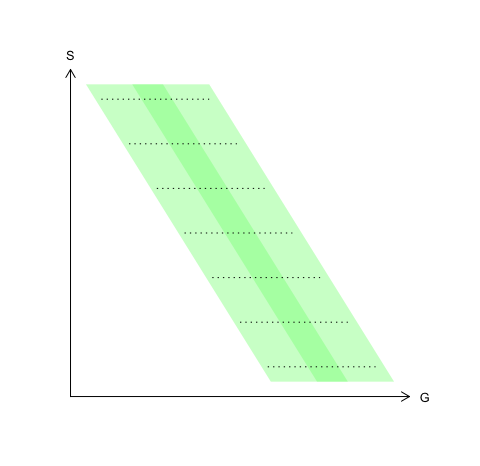
\includegraphics[width=0.5\columnwidth]{correlation-counterexample}
\par\end{centering}
\caption{Correlation counterexample\label{fig:Correlation-counterexample}}

\end{figure}

\hypertarget{proof-of-proposition}{%
\subsection{\texorpdfstring{Proof of Proposition \ref{prop:robustness}}{Proof of Proposition }}\label{proof-of-proposition}}

\begin{proof}

Note that in proposition \ref{prop:prop1}, we took $g_{c(i)} = \bar{g}_{i}$ and $s_{c(i)} = \bar{s}_i$. Write 

\begin{align}
cov(G_{c},S_{c}) & =cov(\bar{G}+\varepsilon^{G},\bar{S}+\varepsilon^{S})\nonumber \\
 & = cov(\bar{G},\bar{S}) + cov(\varepsilon^{G},\bar{S}) + 
     cov(\bar{G},\varepsilon^{S}) + cov(\varepsilon^{G},\varepsilon^{S}).
 \label{eq:cov-with-error}
\end{align}

For any $X$ and $Y$, $cov(X, Y)$ is bounded by $\sqrt{var(X) var(Y)}$.
Plugging $\sigma_{G}^{2}$ and $\sigma_{S}^{2}$ into this formula
shows that under condition 1, $cov(G_{c},S_{c})$ will be arbitrarily
close to $cov(\bar{G},\bar{S})$. Similarly, writing

\[
var(G_{c}) = var(\bar{G}) + var(\varepsilon^{G}) + 2cov(\bar{G},\varepsilon^{G})
\]

shows that $var(G_{c})$ will approach $var(\bar{G})$ as $\sigma_{G}^{2}$
grows small, and similarly for $var(S_{c})$. Plugging these facts
into (\ref{eq:corr-cov-var}) shows that $corr(G_{c},S_{c})$ approaches
$corr(\bar{G},\bar{S})$ as $\sigma_{G}^{2}$ and $\sigma_{S}^{2}$
grow small. Proposition 1 then shows $corr(\bar{G},\bar{S}) < corr(G_{p},S_{p})$
for $k\in(0,1)$.

Under condition 2, $cov(G_{c}, S_{c}) = cov(\bar{G},\bar{S})$ since
the last three terms of the sum in (\ref{eq:cov-with-error}) are
zero. Then since 
\[
cov(\bar{G},\bar{S})\ge cov(G_{p},S_{p}) = 0
\]
with strict inequality iff $k\in(0,1)$, the covariance signs the
correlation. 

\end{proof}

\FloatBarrier

\newpage

\hypertarget{robustness-checks}{%
\subsection{Robustness checks}\label{robustness-checks}}

Table \ref{tab:tbl-bo-psea-no-moth-age} reruns our central regressions,
dropping the control for mother's age at birth. Results show the same
pattern as in the main text: the negative coefficient for birth order
shrinks when controls are added, and then changes sign when university
attendance is added as a potential mediator. However, the birth order
effect is smaller overall, and is never significant.

Table \ref{tab:tbl-bo-psea-dummies} reruns our central regressions but
includes a separate coefficient for each position in the birth order
(with firstborn as the baseline). The basic pattern of our main result
holds: birth order coefficients are negative and increase going down the
birth order; in column 2, adding controls reduces their size; in column
3, adding university attendance reduces their size and significance
still further. Results are slightly messier when we add income, probably
because of the low N. Table \ref{tab:tbl-bo-subset-dummies} runs the
same exercise for different subsets: male respondents, female
respondents, and couples with children.

We also ran a specification with separate birth order dummies within
each family size. Figure \ref{fig:pic-bo-psea-interactions} shows 95\%
confidence intervals for the birth order coefficients, from the column 2
specification including height and IQ controls but no mediators. Most
birth order coefficients are negative (compared to the baseline for the
firstborn) and become more negative as birth order increases. However,
there is some suggestion of a positive ``last born'' effect. This could
happen because last born children receive more attention after elder
children have left home.

Table \ref{tab:tbl-bo-psea-pgs} reruns our regressions controlling for
several polygenic scores. Results are very close to those in the main
text.

Table \ref{tab:tbl-bo-psea-age-fte} reruns relevant columns of Table
\ref{tab:tbl-bo-psea} using age of leaving full-time education as a
measure of educational SES, instead of the university attendance dummy.
Results are similar to those in the main text: controlling for age of
leaving full-time education shrinks the effect of birth order and makes
it insignificant.

Table \ref{tab:tbl-bo-psea-no3} reruns Table \ref{tab:tbl-bo-psea}
excluding families of size 3. Results are very similar to those in the
main text.

 
  \providecommand{\huxb}[2]{\arrayrulecolor[RGB]{#1}\global\arrayrulewidth=#2pt}
  \providecommand{\huxvb}[2]{\color[RGB]{#1}\vrule width #2pt}
  \providecommand{\huxtpad}[1]{\rule{0pt}{#1}}
  \providecommand{\huxbpad}[1]{\rule[-#1]{0pt}{#1}}

\begin{table}[ht]
\begin{centerbox}
\begin{threeparttable}
\captionsetup{justification=centering,singlelinecheck=off}
\caption{\label{tab:tbl-bo-psea-no-moth-age} Regressions of spouse PSEA, without controls for mother's age at respondent's birth}
 \setlength{\tabcolsep}{0pt}
\begin{tabular}{l l l l l l}


\hhline{>{\huxb{0, 0, 0}{0.8}}->{\huxb{0, 0, 0}{0.8}}->{\huxb{0, 0, 0}{0.8}}->{\huxb{0, 0, 0}{0.8}}->{\huxb{0, 0, 0}{0.8}}->{\huxb{0, 0, 0}{0.8}}-}
\arrayrulecolor{black}

\multicolumn{1}{!{\huxvb{0, 0, 0}{0}}c!{\huxvb{0, 0, 0}{0}}}{\huxtpad{6pt + 1em}\centering \hspace{6pt}  \hspace{6pt}\huxbpad{6pt}} &
\multicolumn{1}{c!{\huxvb{0, 0, 0}{0}}}{\huxtpad{6pt + 1em}\centering \hspace{6pt} (1) \hspace{6pt}\huxbpad{6pt}} &
\multicolumn{1}{c!{\huxvb{0, 0, 0}{0}}}{\huxtpad{6pt + 1em}\centering \hspace{6pt} (2) \hspace{6pt}\huxbpad{6pt}} &
\multicolumn{1}{c!{\huxvb{0, 0, 0}{0}}}{\huxtpad{6pt + 1em}\centering \hspace{6pt} (3) \hspace{6pt}\huxbpad{6pt}} &
\multicolumn{1}{c!{\huxvb{0, 0, 0}{0}}}{\huxtpad{6pt + 1em}\centering \hspace{6pt} (4) \hspace{6pt}\huxbpad{6pt}} &
\multicolumn{1}{c!{\huxvb{0, 0, 0}{0}}}{\huxtpad{6pt + 1em}\centering \hspace{6pt} (5) \hspace{6pt}\huxbpad{6pt}} \tabularnewline[-0.5pt]


\hhline{>{\huxb{255, 255, 255}{0.4}}->{\huxb{0, 0, 0}{0.4}}->{\huxb{0, 0, 0}{0.4}}->{\huxb{0, 0, 0}{0.4}}->{\huxb{0, 0, 0}{0.4}}->{\huxb{0, 0, 0}{0.4}}-}
\arrayrulecolor{black}

\multicolumn{1}{!{\huxvb{0, 0, 0}{0}}l!{\huxvb{0, 0, 0}{0}}}{\huxtpad{6pt + 1em}\raggedright \hspace{6pt} Birth order \hspace{6pt}\huxbpad{6pt}} &
\multicolumn{1}{r!{\huxvb{0, 0, 0}{0}}}{\huxtpad{6pt + 1em}\raggedleft \hspace{6pt} -0.0058~~~~ \hspace{6pt}\huxbpad{6pt}} &
\multicolumn{1}{r!{\huxvb{0, 0, 0}{0}}}{\huxtpad{6pt + 1em}\raggedleft \hspace{6pt} -0.0032~~~~ \hspace{6pt}\huxbpad{6pt}} &
\multicolumn{1}{r!{\huxvb{0, 0, 0}{0}}}{\huxtpad{6pt + 1em}\raggedleft \hspace{6pt} 0.0022~~~~ \hspace{6pt}\huxbpad{6pt}} &
\multicolumn{1}{r!{\huxvb{0, 0, 0}{0}}}{\huxtpad{6pt + 1em}\raggedleft \hspace{6pt} -0.0021~~~~ \hspace{6pt}\huxbpad{6pt}} &
\multicolumn{1}{r!{\huxvb{0, 0, 0}{0}}}{\huxtpad{6pt + 1em}\raggedleft \hspace{6pt} 0.0026~~~~ \hspace{6pt}\huxbpad{6pt}} \tabularnewline[-0.5pt]


\hhline{}
\arrayrulecolor{black}

\multicolumn{1}{!{\huxvb{0, 0, 0}{0}}l!{\huxvb{0, 0, 0}{0}}}{\huxtpad{6pt + 1em}\raggedright \hspace{6pt}  \hspace{6pt}\huxbpad{6pt}} &
\multicolumn{1}{r!{\huxvb{0, 0, 0}{0}}}{\huxtpad{6pt + 1em}\raggedleft \hspace{6pt} (0.0126)~~~ \hspace{6pt}\huxbpad{6pt}} &
\multicolumn{1}{r!{\huxvb{0, 0, 0}{0}}}{\huxtpad{6pt + 1em}\raggedleft \hspace{6pt} (0.0128)~~~ \hspace{6pt}\huxbpad{6pt}} &
\multicolumn{1}{r!{\huxvb{0, 0, 0}{0}}}{\huxtpad{6pt + 1em}\raggedleft \hspace{6pt} (0.0127)~~~ \hspace{6pt}\huxbpad{6pt}} &
\multicolumn{1}{r!{\huxvb{0, 0, 0}{0}}}{\huxtpad{6pt + 1em}\raggedleft \hspace{6pt} (0.0128)~~~ \hspace{6pt}\huxbpad{6pt}} &
\multicolumn{1}{r!{\huxvb{0, 0, 0}{0}}}{\huxtpad{6pt + 1em}\raggedleft \hspace{6pt} (0.0127)~~~ \hspace{6pt}\huxbpad{6pt}} \tabularnewline[-0.5pt]


\hhline{}
\arrayrulecolor{black}

\multicolumn{1}{!{\huxvb{0, 0, 0}{0}}l!{\huxvb{0, 0, 0}{0}}}{\huxtpad{6pt + 1em}\raggedright \hspace{6pt} University \hspace{6pt}\huxbpad{6pt}} &
\multicolumn{1}{r!{\huxvb{0, 0, 0}{0}}}{\huxtpad{6pt + 1em}\raggedleft \hspace{6pt} ~~~~~~~~~ \hspace{6pt}\huxbpad{6pt}} &
\multicolumn{1}{r!{\huxvb{0, 0, 0}{0}}}{\huxtpad{6pt + 1em}\raggedleft \hspace{6pt} ~~~~~~~~~ \hspace{6pt}\huxbpad{6pt}} &
\multicolumn{1}{r!{\huxvb{0, 0, 0}{0}}}{\huxtpad{6pt + 1em}\raggedleft \hspace{6pt} 0.2216 *** \hspace{6pt}\huxbpad{6pt}} &
\multicolumn{1}{r!{\huxvb{0, 0, 0}{0}}}{\huxtpad{6pt + 1em}\raggedleft \hspace{6pt} ~~~~~~~~~ \hspace{6pt}\huxbpad{6pt}} &
\multicolumn{1}{r!{\huxvb{0, 0, 0}{0}}}{\huxtpad{6pt + 1em}\raggedleft \hspace{6pt} 0.2090 *** \hspace{6pt}\huxbpad{6pt}} \tabularnewline[-0.5pt]


\hhline{}
\arrayrulecolor{black}

\multicolumn{1}{!{\huxvb{0, 0, 0}{0}}l!{\huxvb{0, 0, 0}{0}}}{\huxtpad{6pt + 1em}\raggedright \hspace{6pt}  \hspace{6pt}\huxbpad{6pt}} &
\multicolumn{1}{r!{\huxvb{0, 0, 0}{0}}}{\huxtpad{6pt + 1em}\raggedleft \hspace{6pt} ~~~~~~~~~ \hspace{6pt}\huxbpad{6pt}} &
\multicolumn{1}{r!{\huxvb{0, 0, 0}{0}}}{\huxtpad{6pt + 1em}\raggedleft \hspace{6pt} ~~~~~~~~~ \hspace{6pt}\huxbpad{6pt}} &
\multicolumn{1}{r!{\huxvb{0, 0, 0}{0}}}{\huxtpad{6pt + 1em}\raggedleft \hspace{6pt} (0.0244)~~~ \hspace{6pt}\huxbpad{6pt}} &
\multicolumn{1}{r!{\huxvb{0, 0, 0}{0}}}{\huxtpad{6pt + 1em}\raggedleft \hspace{6pt} ~~~~~~~~~ \hspace{6pt}\huxbpad{6pt}} &
\multicolumn{1}{r!{\huxvb{0, 0, 0}{0}}}{\huxtpad{6pt + 1em}\raggedleft \hspace{6pt} (0.0249)~~~ \hspace{6pt}\huxbpad{6pt}} \tabularnewline[-0.5pt]


\hhline{}
\arrayrulecolor{black}

\multicolumn{1}{!{\huxvb{0, 0, 0}{0}}l!{\huxvb{0, 0, 0}{0}}}{\huxtpad{6pt + 1em}\raggedright \hspace{6pt} Income \hspace{6pt}\huxbpad{6pt}} &
\multicolumn{1}{r!{\huxvb{0, 0, 0}{0}}}{\huxtpad{6pt + 1em}\raggedleft \hspace{6pt} ~~~~~~~~~ \hspace{6pt}\huxbpad{6pt}} &
\multicolumn{1}{r!{\huxvb{0, 0, 0}{0}}}{\huxtpad{6pt + 1em}\raggedleft \hspace{6pt} ~~~~~~~~~ \hspace{6pt}\huxbpad{6pt}} &
\multicolumn{1}{r!{\huxvb{0, 0, 0}{0}}}{\huxtpad{6pt + 1em}\raggedleft \hspace{6pt} ~~~~~~~~~ \hspace{6pt}\huxbpad{6pt}} &
\multicolumn{1}{r!{\huxvb{0, 0, 0}{0}}}{\huxtpad{6pt + 1em}\raggedleft \hspace{6pt} 0.0032 *** \hspace{6pt}\huxbpad{6pt}} &
\multicolumn{1}{r!{\huxvb{0, 0, 0}{0}}}{\huxtpad{6pt + 1em}\raggedleft \hspace{6pt} 0.0020 **~ \hspace{6pt}\huxbpad{6pt}} \tabularnewline[-0.5pt]


\hhline{}
\arrayrulecolor{black}

\multicolumn{1}{!{\huxvb{0, 0, 0}{0}}l!{\huxvb{0, 0, 0}{0}}}{\huxtpad{6pt + 1em}\raggedright \hspace{6pt}  \hspace{6pt}\huxbpad{6pt}} &
\multicolumn{1}{r!{\huxvb{0, 0, 0}{0}}}{\huxtpad{6pt + 1em}\raggedleft \hspace{6pt} ~~~~~~~~~ \hspace{6pt}\huxbpad{6pt}} &
\multicolumn{1}{r!{\huxvb{0, 0, 0}{0}}}{\huxtpad{6pt + 1em}\raggedleft \hspace{6pt} ~~~~~~~~~ \hspace{6pt}\huxbpad{6pt}} &
\multicolumn{1}{r!{\huxvb{0, 0, 0}{0}}}{\huxtpad{6pt + 1em}\raggedleft \hspace{6pt} ~~~~~~~~~ \hspace{6pt}\huxbpad{6pt}} &
\multicolumn{1}{r!{\huxvb{0, 0, 0}{0}}}{\huxtpad{6pt + 1em}\raggedleft \hspace{6pt} (0.0008)~~~ \hspace{6pt}\huxbpad{6pt}} &
\multicolumn{1}{r!{\huxvb{0, 0, 0}{0}}}{\huxtpad{6pt + 1em}\raggedleft \hspace{6pt} (0.0008)~~~ \hspace{6pt}\huxbpad{6pt}} \tabularnewline[-0.5pt]


\hhline{}
\arrayrulecolor{black}

\multicolumn{1}{!{\huxvb{0, 0, 0}{0}}l!{\huxvb{0, 0, 0}{0}}}{\huxtpad{6pt + 1em}\raggedright \hspace{6pt} Own PSEA \hspace{6pt}\huxbpad{6pt}} &
\multicolumn{1}{r!{\huxvb{0, 0, 0}{0}}}{\huxtpad{6pt + 1em}\raggedleft \hspace{6pt} 0.0579 *** \hspace{6pt}\huxbpad{6pt}} &
\multicolumn{1}{r!{\huxvb{0, 0, 0}{0}}}{\huxtpad{6pt + 1em}\raggedleft \hspace{6pt} 0.0521 *** \hspace{6pt}\huxbpad{6pt}} &
\multicolumn{1}{r!{\huxvb{0, 0, 0}{0}}}{\huxtpad{6pt + 1em}\raggedleft \hspace{6pt} 0.0363 **~ \hspace{6pt}\huxbpad{6pt}} &
\multicolumn{1}{r!{\huxvb{0, 0, 0}{0}}}{\huxtpad{6pt + 1em}\raggedleft \hspace{6pt} 0.0486 *** \hspace{6pt}\huxbpad{6pt}} &
\multicolumn{1}{r!{\huxvb{0, 0, 0}{0}}}{\huxtpad{6pt + 1em}\raggedleft \hspace{6pt} 0.0350 **~ \hspace{6pt}\huxbpad{6pt}} \tabularnewline[-0.5pt]


\hhline{}
\arrayrulecolor{black}

\multicolumn{1}{!{\huxvb{0, 0, 0}{0}}l!{\huxvb{0, 0, 0}{0}}}{\huxtpad{6pt + 1em}\raggedright \hspace{6pt}  \hspace{6pt}\huxbpad{6pt}} &
\multicolumn{1}{r!{\huxvb{0, 0, 0}{0}}}{\huxtpad{6pt + 1em}\raggedleft \hspace{6pt} (0.0117)~~~ \hspace{6pt}\huxbpad{6pt}} &
\multicolumn{1}{r!{\huxvb{0, 0, 0}{0}}}{\huxtpad{6pt + 1em}\raggedleft \hspace{6pt} (0.0118)~~~ \hspace{6pt}\huxbpad{6pt}} &
\multicolumn{1}{r!{\huxvb{0, 0, 0}{0}}}{\huxtpad{6pt + 1em}\raggedleft \hspace{6pt} (0.0119)~~~ \hspace{6pt}\huxbpad{6pt}} &
\multicolumn{1}{r!{\huxvb{0, 0, 0}{0}}}{\huxtpad{6pt + 1em}\raggedleft \hspace{6pt} (0.0119)~~~ \hspace{6pt}\huxbpad{6pt}} &
\multicolumn{1}{r!{\huxvb{0, 0, 0}{0}}}{\huxtpad{6pt + 1em}\raggedleft \hspace{6pt} (0.0119)~~~ \hspace{6pt}\huxbpad{6pt}} \tabularnewline[-0.5pt]


\hhline{}
\arrayrulecolor{black}

\multicolumn{1}{!{\huxvb{0, 0, 0}{0}}l!{\huxvb{0, 0, 0}{0}}}{\huxtpad{6pt + 1em}\raggedright \hspace{6pt} Fluid IQ \hspace{6pt}\huxbpad{6pt}} &
\multicolumn{1}{r!{\huxvb{0, 0, 0}{0}}}{\huxtpad{6pt + 1em}\raggedleft \hspace{6pt} ~~~~~~~~~ \hspace{6pt}\huxbpad{6pt}} &
\multicolumn{1}{r!{\huxvb{0, 0, 0}{0}}}{\huxtpad{6pt + 1em}\raggedleft \hspace{6pt} 0.0197 *** \hspace{6pt}\huxbpad{6pt}} &
\multicolumn{1}{r!{\huxvb{0, 0, 0}{0}}}{\huxtpad{6pt + 1em}\raggedleft \hspace{6pt} 0.0056~~~~ \hspace{6pt}\huxbpad{6pt}} &
\multicolumn{1}{r!{\huxvb{0, 0, 0}{0}}}{\huxtpad{6pt + 1em}\raggedleft \hspace{6pt} 0.0172 **~ \hspace{6pt}\huxbpad{6pt}} &
\multicolumn{1}{r!{\huxvb{0, 0, 0}{0}}}{\huxtpad{6pt + 1em}\raggedleft \hspace{6pt} 0.0048~~~~ \hspace{6pt}\huxbpad{6pt}} \tabularnewline[-0.5pt]


\hhline{}
\arrayrulecolor{black}

\multicolumn{1}{!{\huxvb{0, 0, 0}{0}}l!{\huxvb{0, 0, 0}{0}}}{\huxtpad{6pt + 1em}\raggedright \hspace{6pt}  \hspace{6pt}\huxbpad{6pt}} &
\multicolumn{1}{r!{\huxvb{0, 0, 0}{0}}}{\huxtpad{6pt + 1em}\raggedleft \hspace{6pt} ~~~~~~~~~ \hspace{6pt}\huxbpad{6pt}} &
\multicolumn{1}{r!{\huxvb{0, 0, 0}{0}}}{\huxtpad{6pt + 1em}\raggedleft \hspace{6pt} (0.0059)~~~ \hspace{6pt}\huxbpad{6pt}} &
\multicolumn{1}{r!{\huxvb{0, 0, 0}{0}}}{\huxtpad{6pt + 1em}\raggedleft \hspace{6pt} (0.0061)~~~ \hspace{6pt}\huxbpad{6pt}} &
\multicolumn{1}{r!{\huxvb{0, 0, 0}{0}}}{\huxtpad{6pt + 1em}\raggedleft \hspace{6pt} (0.0060)~~~ \hspace{6pt}\huxbpad{6pt}} &
\multicolumn{1}{r!{\huxvb{0, 0, 0}{0}}}{\huxtpad{6pt + 1em}\raggedleft \hspace{6pt} (0.0062)~~~ \hspace{6pt}\huxbpad{6pt}} \tabularnewline[-0.5pt]


\hhline{}
\arrayrulecolor{black}

\multicolumn{1}{!{\huxvb{0, 0, 0}{0}}l!{\huxvb{0, 0, 0}{0}}}{\huxtpad{6pt + 1em}\raggedright \hspace{6pt} Height \hspace{6pt}\huxbpad{6pt}} &
\multicolumn{1}{r!{\huxvb{0, 0, 0}{0}}}{\huxtpad{6pt + 1em}\raggedleft \hspace{6pt} ~~~~~~~~~ \hspace{6pt}\huxbpad{6pt}} &
\multicolumn{1}{r!{\huxvb{0, 0, 0}{0}}}{\huxtpad{6pt + 1em}\raggedleft \hspace{6pt} 0.0052 *** \hspace{6pt}\huxbpad{6pt}} &
\multicolumn{1}{r!{\huxvb{0, 0, 0}{0}}}{\huxtpad{6pt + 1em}\raggedleft \hspace{6pt} 0.0043 *** \hspace{6pt}\huxbpad{6pt}} &
\multicolumn{1}{r!{\huxvb{0, 0, 0}{0}}}{\huxtpad{6pt + 1em}\raggedleft \hspace{6pt} 0.0041 **~ \hspace{6pt}\huxbpad{6pt}} &
\multicolumn{1}{r!{\huxvb{0, 0, 0}{0}}}{\huxtpad{6pt + 1em}\raggedleft \hspace{6pt} 0.0036 **~ \hspace{6pt}\huxbpad{6pt}} \tabularnewline[-0.5pt]


\hhline{}
\arrayrulecolor{black}

\multicolumn{1}{!{\huxvb{0, 0, 0}{0}}l!{\huxvb{0, 0, 0}{0}}}{\huxtpad{6pt + 1em}\raggedright \hspace{6pt}  \hspace{6pt}\huxbpad{6pt}} &
\multicolumn{1}{r!{\huxvb{0, 0, 0}{0}}}{\huxtpad{6pt + 1em}\raggedleft \hspace{6pt} ~~~~~~~~~ \hspace{6pt}\huxbpad{6pt}} &
\multicolumn{1}{r!{\huxvb{0, 0, 0}{0}}}{\huxtpad{6pt + 1em}\raggedleft \hspace{6pt} (0.0012)~~~ \hspace{6pt}\huxbpad{6pt}} &
\multicolumn{1}{r!{\huxvb{0, 0, 0}{0}}}{\huxtpad{6pt + 1em}\raggedleft \hspace{6pt} (0.0012)~~~ \hspace{6pt}\huxbpad{6pt}} &
\multicolumn{1}{r!{\huxvb{0, 0, 0}{0}}}{\huxtpad{6pt + 1em}\raggedleft \hspace{6pt} (0.0013)~~~ \hspace{6pt}\huxbpad{6pt}} &
\multicolumn{1}{r!{\huxvb{0, 0, 0}{0}}}{\huxtpad{6pt + 1em}\raggedleft \hspace{6pt} (0.0012)~~~ \hspace{6pt}\huxbpad{6pt}} \tabularnewline[-0.5pt]


\hhline{>{\huxb{255, 255, 255}{0.4}}->{\huxb{0, 0, 0}{0.4}}->{\huxb{0, 0, 0}{0.4}}->{\huxb{0, 0, 0}{0.4}}->{\huxb{0, 0, 0}{0.4}}->{\huxb{0, 0, 0}{0.4}}-}
\arrayrulecolor{black}

\multicolumn{1}{!{\huxvb{0, 0, 0}{0}}l!{\huxvb{0, 0, 0}{0}}}{\huxtpad{6pt + 1em}\raggedright \hspace{6pt} Family size dummies \hspace{6pt}\huxbpad{6pt}} &
\multicolumn{1}{r!{\huxvb{0, 0, 0}{0}}}{\huxtpad{6pt + 1em}\raggedleft \hspace{6pt} Yes~~~~~~~~~ \hspace{6pt}\huxbpad{6pt}} &
\multicolumn{1}{r!{\huxvb{0, 0, 0}{0}}}{\huxtpad{6pt + 1em}\raggedleft \hspace{6pt} Yes~~~~~~~~~ \hspace{6pt}\huxbpad{6pt}} &
\multicolumn{1}{r!{\huxvb{0, 0, 0}{0}}}{\huxtpad{6pt + 1em}\raggedleft \hspace{6pt} Yes~~~~~~~~~ \hspace{6pt}\huxbpad{6pt}} &
\multicolumn{1}{r!{\huxvb{0, 0, 0}{0}}}{\huxtpad{6pt + 1em}\raggedleft \hspace{6pt} Yes~~~~~~~~~ \hspace{6pt}\huxbpad{6pt}} &
\multicolumn{1}{r!{\huxvb{0, 0, 0}{0}}}{\huxtpad{6pt + 1em}\raggedleft \hspace{6pt} Yes~~~~~~~~~ \hspace{6pt}\huxbpad{6pt}} \tabularnewline[-0.5pt]


\hhline{}
\arrayrulecolor{black}

\multicolumn{1}{!{\huxvb{0, 0, 0}{0}}l!{\huxvb{0, 0, 0}{0}}}{\huxtpad{6pt + 1em}\raggedright \hspace{6pt} Birth month dummies \hspace{6pt}\huxbpad{6pt}} &
\multicolumn{1}{r!{\huxvb{0, 0, 0}{0}}}{\huxtpad{6pt + 1em}\raggedleft \hspace{6pt} Yes~~~~~~~~~ \hspace{6pt}\huxbpad{6pt}} &
\multicolumn{1}{r!{\huxvb{0, 0, 0}{0}}}{\huxtpad{6pt + 1em}\raggedleft \hspace{6pt} Yes~~~~~~~~~ \hspace{6pt}\huxbpad{6pt}} &
\multicolumn{1}{r!{\huxvb{0, 0, 0}{0}}}{\huxtpad{6pt + 1em}\raggedleft \hspace{6pt} Yes~~~~~~~~~ \hspace{6pt}\huxbpad{6pt}} &
\multicolumn{1}{r!{\huxvb{0, 0, 0}{0}}}{\huxtpad{6pt + 1em}\raggedleft \hspace{6pt} Yes~~~~~~~~~ \hspace{6pt}\huxbpad{6pt}} &
\multicolumn{1}{r!{\huxvb{0, 0, 0}{0}}}{\huxtpad{6pt + 1em}\raggedleft \hspace{6pt} Yes~~~~~~~~~ \hspace{6pt}\huxbpad{6pt}} \tabularnewline[-0.5pt]


\hhline{}
\arrayrulecolor{black}

\multicolumn{1}{!{\huxvb{0, 0, 0}{0}}l!{\huxvb{0, 0, 0}{0}}}{\huxtpad{6pt + 1em}\raggedright \hspace{6pt} Birth year dummies \hspace{6pt}\huxbpad{6pt}} &
\multicolumn{1}{r!{\huxvb{0, 0, 0}{0}}}{\huxtpad{6pt + 1em}\raggedleft \hspace{6pt} Yes~~~~~~~~~ \hspace{6pt}\huxbpad{6pt}} &
\multicolumn{1}{r!{\huxvb{0, 0, 0}{0}}}{\huxtpad{6pt + 1em}\raggedleft \hspace{6pt} Yes~~~~~~~~~ \hspace{6pt}\huxbpad{6pt}} &
\multicolumn{1}{r!{\huxvb{0, 0, 0}{0}}}{\huxtpad{6pt + 1em}\raggedleft \hspace{6pt} Yes~~~~~~~~~ \hspace{6pt}\huxbpad{6pt}} &
\multicolumn{1}{r!{\huxvb{0, 0, 0}{0}}}{\huxtpad{6pt + 1em}\raggedleft \hspace{6pt} Yes~~~~~~~~~ \hspace{6pt}\huxbpad{6pt}} &
\multicolumn{1}{r!{\huxvb{0, 0, 0}{0}}}{\huxtpad{6pt + 1em}\raggedleft \hspace{6pt} Yes~~~~~~~~~ \hspace{6pt}\huxbpad{6pt}} \tabularnewline[-0.5pt]


\hhline{>{\huxb{255, 255, 255}{0.4}}->{\huxb{0, 0, 0}{0.4}}->{\huxb{0, 0, 0}{0.4}}->{\huxb{0, 0, 0}{0.4}}->{\huxb{0, 0, 0}{0.4}}->{\huxb{0, 0, 0}{0.4}}-}
\arrayrulecolor{black}

\multicolumn{1}{!{\huxvb{0, 0, 0}{0}}l!{\huxvb{0, 0, 0}{0}}}{\huxtpad{6pt + 1em}\raggedright \hspace{6pt} N \hspace{6pt}\huxbpad{6pt}} &
\multicolumn{1}{r!{\huxvb{0, 0, 0}{0}}}{\huxtpad{6pt + 1em}\raggedleft \hspace{6pt} 8017~~~~~~~~~ \hspace{6pt}\huxbpad{6pt}} &
\multicolumn{1}{r!{\huxvb{0, 0, 0}{0}}}{\huxtpad{6pt + 1em}\raggedleft \hspace{6pt} 7868~~~~~~~~~ \hspace{6pt}\huxbpad{6pt}} &
\multicolumn{1}{r!{\huxvb{0, 0, 0}{0}}}{\huxtpad{6pt + 1em}\raggedleft \hspace{6pt} 7868~~~~~~~~~ \hspace{6pt}\huxbpad{6pt}} &
\multicolumn{1}{r!{\huxvb{0, 0, 0}{0}}}{\huxtpad{6pt + 1em}\raggedleft \hspace{6pt} 7868~~~~~~~~~ \hspace{6pt}\huxbpad{6pt}} &
\multicolumn{1}{r!{\huxvb{0, 0, 0}{0}}}{\huxtpad{6pt + 1em}\raggedleft \hspace{6pt} 7868~~~~~~~~~ \hspace{6pt}\huxbpad{6pt}} \tabularnewline[-0.5pt]


\hhline{}
\arrayrulecolor{black}

\multicolumn{1}{!{\huxvb{0, 0, 0}{0}}l!{\huxvb{0, 0, 0}{0}}}{\huxtpad{6pt + 1em}\raggedright \hspace{6pt} R2 \hspace{6pt}\huxbpad{6pt}} &
\multicolumn{1}{r!{\huxvb{0, 0, 0}{0}}}{\huxtpad{6pt + 1em}\raggedleft \hspace{6pt} 0.011~~~~~ \hspace{6pt}\huxbpad{6pt}} &
\multicolumn{1}{r!{\huxvb{0, 0, 0}{0}}}{\huxtpad{6pt + 1em}\raggedleft \hspace{6pt} 0.015~~~~~ \hspace{6pt}\huxbpad{6pt}} &
\multicolumn{1}{r!{\huxvb{0, 0, 0}{0}}}{\huxtpad{6pt + 1em}\raggedleft \hspace{6pt} 0.026~~~~~ \hspace{6pt}\huxbpad{6pt}} &
\multicolumn{1}{r!{\huxvb{0, 0, 0}{0}}}{\huxtpad{6pt + 1em}\raggedleft \hspace{6pt} 0.017~~~~~ \hspace{6pt}\huxbpad{6pt}} &
\multicolumn{1}{r!{\huxvb{0, 0, 0}{0}}}{\huxtpad{6pt + 1em}\raggedleft \hspace{6pt} 0.026~~~~~ \hspace{6pt}\huxbpad{6pt}} \tabularnewline[-0.5pt]


\hhline{}
\arrayrulecolor{black}

\multicolumn{1}{!{\huxvb{0, 0, 0}{0}}l!{\huxvb{0, 0, 0}{0}}}{\huxtpad{6pt + 1em}\raggedright \hspace{6pt} logLik \hspace{6pt}\huxbpad{6pt}} &
\multicolumn{1}{r!{\huxvb{0, 0, 0}{0}}}{\huxtpad{6pt + 1em}\raggedleft \hspace{6pt} -11292.019~~~~~ \hspace{6pt}\huxbpad{6pt}} &
\multicolumn{1}{r!{\huxvb{0, 0, 0}{0}}}{\huxtpad{6pt + 1em}\raggedleft \hspace{6pt} -11062.255~~~~~ \hspace{6pt}\huxbpad{6pt}} &
\multicolumn{1}{r!{\huxvb{0, 0, 0}{0}}}{\huxtpad{6pt + 1em}\raggedleft \hspace{6pt} -11019.983~~~~~ \hspace{6pt}\huxbpad{6pt}} &
\multicolumn{1}{r!{\huxvb{0, 0, 0}{0}}}{\huxtpad{6pt + 1em}\raggedleft \hspace{6pt} -11052.559~~~~~ \hspace{6pt}\huxbpad{6pt}} &
\multicolumn{1}{r!{\huxvb{0, 0, 0}{0}}}{\huxtpad{6pt + 1em}\raggedleft \hspace{6pt} -11016.175~~~~~ \hspace{6pt}\huxbpad{6pt}} \tabularnewline[-0.5pt]


\hhline{}
\arrayrulecolor{black}

\multicolumn{1}{!{\huxvb{0, 0, 0}{0}}l!{\huxvb{0, 0, 0}{0}}}{\huxtpad{6pt + 1em}\raggedright \hspace{6pt} AIC \hspace{6pt}\huxbpad{6pt}} &
\multicolumn{1}{r!{\huxvb{0, 0, 0}{0}}}{\huxtpad{6pt + 1em}\raggedleft \hspace{6pt} 22688.039~~~~~ \hspace{6pt}\huxbpad{6pt}} &
\multicolumn{1}{r!{\huxvb{0, 0, 0}{0}}}{\huxtpad{6pt + 1em}\raggedleft \hspace{6pt} 22232.511~~~~~ \hspace{6pt}\huxbpad{6pt}} &
\multicolumn{1}{r!{\huxvb{0, 0, 0}{0}}}{\huxtpad{6pt + 1em}\raggedleft \hspace{6pt} 22149.966~~~~~ \hspace{6pt}\huxbpad{6pt}} &
\multicolumn{1}{r!{\huxvb{0, 0, 0}{0}}}{\huxtpad{6pt + 1em}\raggedleft \hspace{6pt} 22215.118~~~~~ \hspace{6pt}\huxbpad{6pt}} &
\multicolumn{1}{r!{\huxvb{0, 0, 0}{0}}}{\huxtpad{6pt + 1em}\raggedleft \hspace{6pt} 22144.351~~~~~ \hspace{6pt}\huxbpad{6pt}} \tabularnewline[-0.5pt]


\hhline{>{\huxb{0, 0, 0}{0.8}}->{\huxb{0, 0, 0}{0.8}}->{\huxb{0, 0, 0}{0.8}}->{\huxb{0, 0, 0}{0.8}}->{\huxb{0, 0, 0}{0.8}}->{\huxb{0, 0, 0}{0.8}}-}
\arrayrulecolor{black}

\multicolumn{6}{!{\huxvb{0, 0, 0}{0}}l!{\huxvb{0, 0, 0}{0}}}{\huxtpad{6pt + 1em}\raggedright \hspace{6pt}  *** p $<$ 0.001;  ** p $<$ 0.01;  * p $<$ 0.05;  + p $<$ 0.1. Standard errors: robust. \hspace{6pt}\huxbpad{6pt}} \tabularnewline[-0.5pt]


\hhline{}
\arrayrulecolor{black}
\end{tabular}
\end{threeparttable}\par\end{centerbox}

\end{table}
 

 
  \providecommand{\huxb}[2]{\arrayrulecolor[RGB]{#1}\global\arrayrulewidth=#2pt}
  \providecommand{\huxvb}[2]{\color[RGB]{#1}\vrule width #2pt}
  \providecommand{\huxtpad}[1]{\rule{0pt}{#1}}
  \providecommand{\huxbpad}[1]{\rule[-#1]{0pt}{#1}}

\begin{table}[ht]
\begin{centerbox}
\begin{threeparttable}
\captionsetup{justification=centering,singlelinecheck=off}
\caption{\label{tab:tbl-bo-psea-dummies} Regressions of spouse PSEA, separate birth order coefficient dummies}
 \setlength{\tabcolsep}{0pt}
\begin{tabular}{l l l l l l}


\hhline{>{\huxb{0, 0, 0}{0.8}}->{\huxb{0, 0, 0}{0.8}}->{\huxb{0, 0, 0}{0.8}}->{\huxb{0, 0, 0}{0.8}}->{\huxb{0, 0, 0}{0.8}}->{\huxb{0, 0, 0}{0.8}}-}
\arrayrulecolor{black}

\multicolumn{1}{!{\huxvb{0, 0, 0}{0}}c!{\huxvb{0, 0, 0}{0}}}{\huxtpad{3pt + 1em}\centering \hspace{6pt} {\fontsize{10pt}{12pt}\selectfont } \hspace{6pt}\huxbpad{3pt}} &
\multicolumn{1}{c!{\huxvb{0, 0, 0}{0}}}{\huxtpad{3pt + 1em}\centering \hspace{6pt} {\fontsize{10pt}{12pt}\selectfont (1)} \hspace{6pt}\huxbpad{3pt}} &
\multicolumn{1}{c!{\huxvb{0, 0, 0}{0}}}{\huxtpad{3pt + 1em}\centering \hspace{6pt} {\fontsize{10pt}{12pt}\selectfont (2)} \hspace{6pt}\huxbpad{3pt}} &
\multicolumn{1}{c!{\huxvb{0, 0, 0}{0}}}{\huxtpad{3pt + 1em}\centering \hspace{6pt} {\fontsize{10pt}{12pt}\selectfont (3)} \hspace{6pt}\huxbpad{3pt}} &
\multicolumn{1}{c!{\huxvb{0, 0, 0}{0}}}{\huxtpad{3pt + 1em}\centering \hspace{6pt} {\fontsize{10pt}{12pt}\selectfont (4)} \hspace{6pt}\huxbpad{3pt}} &
\multicolumn{1}{c!{\huxvb{0, 0, 0}{0}}}{\huxtpad{3pt + 1em}\centering \hspace{6pt} {\fontsize{10pt}{12pt}\selectfont (5)} \hspace{6pt}\huxbpad{3pt}} \tabularnewline[-0.5pt]


\hhline{>{\huxb{255, 255, 255}{0.4}}->{\huxb{0, 0, 0}{0.4}}->{\huxb{0, 0, 0}{0.4}}->{\huxb{0, 0, 0}{0.4}}->{\huxb{0, 0, 0}{0.4}}->{\huxb{0, 0, 0}{0.4}}-}
\arrayrulecolor{black}

\multicolumn{1}{!{\huxvb{0, 0, 0}{0}}l!{\huxvb{0, 0, 0}{0}}}{\huxtpad{3pt + 1em}\raggedright \hspace{6pt} {\fontsize{10pt}{12pt}\selectfont Birth order 2} \hspace{6pt}\huxbpad{3pt}} &
\multicolumn{1}{r!{\huxvb{0, 0, 0}{0}}}{\huxtpad{3pt + 1em}\raggedleft \hspace{6pt} {\fontsize{10pt}{12pt}\selectfont -0.0573 *~~} \hspace{6pt}\huxbpad{3pt}} &
\multicolumn{1}{r!{\huxvb{0, 0, 0}{0}}}{\huxtpad{3pt + 1em}\raggedleft \hspace{6pt} {\fontsize{10pt}{12pt}\selectfont -0.0369~~~~} \hspace{6pt}\huxbpad{3pt}} &
\multicolumn{1}{r!{\huxvb{0, 0, 0}{0}}}{\huxtpad{3pt + 1em}\raggedleft \hspace{6pt} {\fontsize{10pt}{12pt}\selectfont -0.0239~~~~} \hspace{6pt}\huxbpad{3pt}} &
\multicolumn{1}{r!{\huxvb{0, 0, 0}{0}}}{\huxtpad{3pt + 1em}\raggedleft \hspace{6pt} {\fontsize{10pt}{12pt}\selectfont -0.0389~~~} \hspace{6pt}\huxbpad{3pt}} &
\multicolumn{1}{r!{\huxvb{0, 0, 0}{0}}}{\huxtpad{3pt + 1em}\raggedleft \hspace{6pt} {\fontsize{10pt}{12pt}\selectfont -0.0379~~~~} \hspace{6pt}\huxbpad{3pt}} \tabularnewline[-0.5pt]


\hhline{}
\arrayrulecolor{black}

\multicolumn{1}{!{\huxvb{0, 0, 0}{0}}l!{\huxvb{0, 0, 0}{0}}}{\huxtpad{3pt + 1em}\raggedright \hspace{6pt} {\fontsize{10pt}{12pt}\selectfont } \hspace{6pt}\huxbpad{3pt}} &
\multicolumn{1}{r!{\huxvb{0, 0, 0}{0}}}{\huxtpad{3pt + 1em}\raggedleft \hspace{6pt} {\fontsize{10pt}{12pt}\selectfont (0.0248)~~~} \hspace{6pt}\huxbpad{3pt}} &
\multicolumn{1}{r!{\huxvb{0, 0, 0}{0}}}{\huxtpad{3pt + 1em}\raggedleft \hspace{6pt} {\fontsize{10pt}{12pt}\selectfont (0.0252)~~~} \hspace{6pt}\huxbpad{3pt}} &
\multicolumn{1}{r!{\huxvb{0, 0, 0}{0}}}{\huxtpad{3pt + 1em}\raggedleft \hspace{6pt} {\fontsize{10pt}{12pt}\selectfont (0.0251)~~~} \hspace{6pt}\huxbpad{3pt}} &
\multicolumn{1}{r!{\huxvb{0, 0, 0}{0}}}{\huxtpad{3pt + 1em}\raggedleft \hspace{6pt} {\fontsize{10pt}{12pt}\selectfont (0.0445)~~} \hspace{6pt}\huxbpad{3pt}} &
\multicolumn{1}{r!{\huxvb{0, 0, 0}{0}}}{\huxtpad{3pt + 1em}\raggedleft \hspace{6pt} {\fontsize{10pt}{12pt}\selectfont (0.0444)~~~} \hspace{6pt}\huxbpad{3pt}} \tabularnewline[-0.5pt]


\hhline{}
\arrayrulecolor{black}

\multicolumn{1}{!{\huxvb{0, 0, 0}{0}}l!{\huxvb{0, 0, 0}{0}}}{\huxtpad{3pt + 1em}\raggedright \hspace{6pt} {\fontsize{10pt}{12pt}\selectfont Birth order 3} \hspace{6pt}\huxbpad{3pt}} &
\multicolumn{1}{r!{\huxvb{0, 0, 0}{0}}}{\huxtpad{3pt + 1em}\raggedleft \hspace{6pt} {\fontsize{10pt}{12pt}\selectfont -0.0841 *~~} \hspace{6pt}\huxbpad{3pt}} &
\multicolumn{1}{r!{\huxvb{0, 0, 0}{0}}}{\huxtpad{3pt + 1em}\raggedleft \hspace{6pt} {\fontsize{10pt}{12pt}\selectfont -0.0545~~~~} \hspace{6pt}\huxbpad{3pt}} &
\multicolumn{1}{r!{\huxvb{0, 0, 0}{0}}}{\huxtpad{3pt + 1em}\raggedleft \hspace{6pt} {\fontsize{10pt}{12pt}\selectfont -0.0264~~~~} \hspace{6pt}\huxbpad{3pt}} &
\multicolumn{1}{r!{\huxvb{0, 0, 0}{0}}}{\huxtpad{3pt + 1em}\raggedleft \hspace{6pt} {\fontsize{10pt}{12pt}\selectfont 0.0008~~~} \hspace{6pt}\huxbpad{3pt}} &
\multicolumn{1}{r!{\huxvb{0, 0, 0}{0}}}{\huxtpad{3pt + 1em}\raggedleft \hspace{6pt} {\fontsize{10pt}{12pt}\selectfont 0.0197~~~~} \hspace{6pt}\huxbpad{3pt}} \tabularnewline[-0.5pt]


\hhline{}
\arrayrulecolor{black}

\multicolumn{1}{!{\huxvb{0, 0, 0}{0}}l!{\huxvb{0, 0, 0}{0}}}{\huxtpad{3pt + 1em}\raggedright \hspace{6pt} {\fontsize{10pt}{12pt}\selectfont } \hspace{6pt}\huxbpad{3pt}} &
\multicolumn{1}{r!{\huxvb{0, 0, 0}{0}}}{\huxtpad{3pt + 1em}\raggedleft \hspace{6pt} {\fontsize{10pt}{12pt}\selectfont (0.0411)~~~} \hspace{6pt}\huxbpad{3pt}} &
\multicolumn{1}{r!{\huxvb{0, 0, 0}{0}}}{\huxtpad{3pt + 1em}\raggedleft \hspace{6pt} {\fontsize{10pt}{12pt}\selectfont (0.0415)~~~} \hspace{6pt}\huxbpad{3pt}} &
\multicolumn{1}{r!{\huxvb{0, 0, 0}{0}}}{\huxtpad{3pt + 1em}\raggedleft \hspace{6pt} {\fontsize{10pt}{12pt}\selectfont (0.0413)~~~} \hspace{6pt}\huxbpad{3pt}} &
\multicolumn{1}{r!{\huxvb{0, 0, 0}{0}}}{\huxtpad{3pt + 1em}\raggedleft \hspace{6pt} {\fontsize{10pt}{12pt}\selectfont (0.0737)~~} \hspace{6pt}\huxbpad{3pt}} &
\multicolumn{1}{r!{\huxvb{0, 0, 0}{0}}}{\huxtpad{3pt + 1em}\raggedleft \hspace{6pt} {\fontsize{10pt}{12pt}\selectfont (0.0734)~~~} \hspace{6pt}\huxbpad{3pt}} \tabularnewline[-0.5pt]


\hhline{}
\arrayrulecolor{black}

\multicolumn{1}{!{\huxvb{0, 0, 0}{0}}l!{\huxvb{0, 0, 0}{0}}}{\huxtpad{3pt + 1em}\raggedright \hspace{6pt} {\fontsize{10pt}{12pt}\selectfont Birth order 4} \hspace{6pt}\huxbpad{3pt}} &
\multicolumn{1}{r!{\huxvb{0, 0, 0}{0}}}{\huxtpad{3pt + 1em}\raggedleft \hspace{6pt} {\fontsize{10pt}{12pt}\selectfont -0.0451~~~~} \hspace{6pt}\huxbpad{3pt}} &
\multicolumn{1}{r!{\huxvb{0, 0, 0}{0}}}{\huxtpad{3pt + 1em}\raggedleft \hspace{6pt} {\fontsize{10pt}{12pt}\selectfont 0.0062~~~~} \hspace{6pt}\huxbpad{3pt}} &
\multicolumn{1}{r!{\huxvb{0, 0, 0}{0}}}{\huxtpad{3pt + 1em}\raggedleft \hspace{6pt} {\fontsize{10pt}{12pt}\selectfont 0.0499~~~~} \hspace{6pt}\huxbpad{3pt}} &
\multicolumn{1}{r!{\huxvb{0, 0, 0}{0}}}{\huxtpad{3pt + 1em}\raggedleft \hspace{6pt} {\fontsize{10pt}{12pt}\selectfont 0.0529~~~} \hspace{6pt}\huxbpad{3pt}} &
\multicolumn{1}{r!{\huxvb{0, 0, 0}{0}}}{\huxtpad{3pt + 1em}\raggedleft \hspace{6pt} {\fontsize{10pt}{12pt}\selectfont 0.0728~~~~} \hspace{6pt}\huxbpad{3pt}} \tabularnewline[-0.5pt]


\hhline{}
\arrayrulecolor{black}

\multicolumn{1}{!{\huxvb{0, 0, 0}{0}}l!{\huxvb{0, 0, 0}{0}}}{\huxtpad{3pt + 1em}\raggedright \hspace{6pt} {\fontsize{10pt}{12pt}\selectfont } \hspace{6pt}\huxbpad{3pt}} &
\multicolumn{1}{r!{\huxvb{0, 0, 0}{0}}}{\huxtpad{3pt + 1em}\raggedleft \hspace{6pt} {\fontsize{10pt}{12pt}\selectfont (0.0696)~~~} \hspace{6pt}\huxbpad{3pt}} &
\multicolumn{1}{r!{\huxvb{0, 0, 0}{0}}}{\huxtpad{3pt + 1em}\raggedleft \hspace{6pt} {\fontsize{10pt}{12pt}\selectfont (0.0709)~~~} \hspace{6pt}\huxbpad{3pt}} &
\multicolumn{1}{r!{\huxvb{0, 0, 0}{0}}}{\huxtpad{3pt + 1em}\raggedleft \hspace{6pt} {\fontsize{10pt}{12pt}\selectfont (0.0711)~~~} \hspace{6pt}\huxbpad{3pt}} &
\multicolumn{1}{r!{\huxvb{0, 0, 0}{0}}}{\huxtpad{3pt + 1em}\raggedleft \hspace{6pt} {\fontsize{10pt}{12pt}\selectfont (0.1295)~~} \hspace{6pt}\huxbpad{3pt}} &
\multicolumn{1}{r!{\huxvb{0, 0, 0}{0}}}{\huxtpad{3pt + 1em}\raggedleft \hspace{6pt} {\fontsize{10pt}{12pt}\selectfont (0.1302)~~~} \hspace{6pt}\huxbpad{3pt}} \tabularnewline[-0.5pt]


\hhline{}
\arrayrulecolor{black}

\multicolumn{1}{!{\huxvb{0, 0, 0}{0}}l!{\huxvb{0, 0, 0}{0}}}{\huxtpad{3pt + 1em}\raggedright \hspace{6pt} {\fontsize{10pt}{12pt}\selectfont Birth order 5} \hspace{6pt}\huxbpad{3pt}} &
\multicolumn{1}{r!{\huxvb{0, 0, 0}{0}}}{\huxtpad{3pt + 1em}\raggedleft \hspace{6pt} {\fontsize{10pt}{12pt}\selectfont 0.0015~~~~} \hspace{6pt}\huxbpad{3pt}} &
\multicolumn{1}{r!{\huxvb{0, 0, 0}{0}}}{\huxtpad{3pt + 1em}\raggedleft \hspace{6pt} {\fontsize{10pt}{12pt}\selectfont 0.0358~~~~} \hspace{6pt}\huxbpad{3pt}} &
\multicolumn{1}{r!{\huxvb{0, 0, 0}{0}}}{\huxtpad{3pt + 1em}\raggedleft \hspace{6pt} {\fontsize{10pt}{12pt}\selectfont 0.0796~~~~} \hspace{6pt}\huxbpad{3pt}} &
\multicolumn{1}{r!{\huxvb{0, 0, 0}{0}}}{\huxtpad{3pt + 1em}\raggedleft \hspace{6pt} {\fontsize{10pt}{12pt}\selectfont 0.4368 +~} \hspace{6pt}\huxbpad{3pt}} &
\multicolumn{1}{r!{\huxvb{0, 0, 0}{0}}}{\huxtpad{3pt + 1em}\raggedleft \hspace{6pt} {\fontsize{10pt}{12pt}\selectfont 0.4608 +~~} \hspace{6pt}\huxbpad{3pt}} \tabularnewline[-0.5pt]


\hhline{}
\arrayrulecolor{black}

\multicolumn{1}{!{\huxvb{0, 0, 0}{0}}l!{\huxvb{0, 0, 0}{0}}}{\huxtpad{3pt + 1em}\raggedright \hspace{6pt} {\fontsize{10pt}{12pt}\selectfont } \hspace{6pt}\huxbpad{3pt}} &
\multicolumn{1}{r!{\huxvb{0, 0, 0}{0}}}{\huxtpad{3pt + 1em}\raggedleft \hspace{6pt} {\fontsize{10pt}{12pt}\selectfont (0.1197)~~~} \hspace{6pt}\huxbpad{3pt}} &
\multicolumn{1}{r!{\huxvb{0, 0, 0}{0}}}{\huxtpad{3pt + 1em}\raggedleft \hspace{6pt} {\fontsize{10pt}{12pt}\selectfont (0.1228)~~~} \hspace{6pt}\huxbpad{3pt}} &
\multicolumn{1}{r!{\huxvb{0, 0, 0}{0}}}{\huxtpad{3pt + 1em}\raggedleft \hspace{6pt} {\fontsize{10pt}{12pt}\selectfont (0.1228)~~~} \hspace{6pt}\huxbpad{3pt}} &
\multicolumn{1}{r!{\huxvb{0, 0, 0}{0}}}{\huxtpad{3pt + 1em}\raggedleft \hspace{6pt} {\fontsize{10pt}{12pt}\selectfont (0.2587)~~} \hspace{6pt}\huxbpad{3pt}} &
\multicolumn{1}{r!{\huxvb{0, 0, 0}{0}}}{\huxtpad{3pt + 1em}\raggedleft \hspace{6pt} {\fontsize{10pt}{12pt}\selectfont (0.2618)~~~} \hspace{6pt}\huxbpad{3pt}} \tabularnewline[-0.5pt]


\hhline{}
\arrayrulecolor{black}

\multicolumn{1}{!{\huxvb{0, 0, 0}{0}}l!{\huxvb{0, 0, 0}{0}}}{\huxtpad{3pt + 1em}\raggedright \hspace{6pt} {\fontsize{10pt}{12pt}\selectfont Birth order 6} \hspace{6pt}\huxbpad{3pt}} &
\multicolumn{1}{r!{\huxvb{0, 0, 0}{0}}}{\huxtpad{3pt + 1em}\raggedleft \hspace{6pt} {\fontsize{10pt}{12pt}\selectfont -0.2347~~~~} \hspace{6pt}\huxbpad{3pt}} &
\multicolumn{1}{r!{\huxvb{0, 0, 0}{0}}}{\huxtpad{3pt + 1em}\raggedleft \hspace{6pt} {\fontsize{10pt}{12pt}\selectfont -0.1906~~~~} \hspace{6pt}\huxbpad{3pt}} &
\multicolumn{1}{r!{\huxvb{0, 0, 0}{0}}}{\huxtpad{3pt + 1em}\raggedleft \hspace{6pt} {\fontsize{10pt}{12pt}\selectfont -0.1572~~~~} \hspace{6pt}\huxbpad{3pt}} &
\multicolumn{1}{r!{\huxvb{0, 0, 0}{0}}}{\huxtpad{3pt + 1em}\raggedleft \hspace{6pt} {\fontsize{10pt}{12pt}\selectfont 0.6275 **} \hspace{6pt}\huxbpad{3pt}} &
\multicolumn{1}{r!{\huxvb{0, 0, 0}{0}}}{\huxtpad{3pt + 1em}\raggedleft \hspace{6pt} {\fontsize{10pt}{12pt}\selectfont 0.6500 **~} \hspace{6pt}\huxbpad{3pt}} \tabularnewline[-0.5pt]


\hhline{}
\arrayrulecolor{black}

\multicolumn{1}{!{\huxvb{0, 0, 0}{0}}l!{\huxvb{0, 0, 0}{0}}}{\huxtpad{3pt + 1em}\raggedright \hspace{6pt} {\fontsize{10pt}{12pt}\selectfont } \hspace{6pt}\huxbpad{3pt}} &
\multicolumn{1}{r!{\huxvb{0, 0, 0}{0}}}{\huxtpad{3pt + 1em}\raggedleft \hspace{6pt} {\fontsize{10pt}{12pt}\selectfont (0.2059)~~~} \hspace{6pt}\huxbpad{3pt}} &
\multicolumn{1}{r!{\huxvb{0, 0, 0}{0}}}{\huxtpad{3pt + 1em}\raggedleft \hspace{6pt} {\fontsize{10pt}{12pt}\selectfont (0.2035)~~~} \hspace{6pt}\huxbpad{3pt}} &
\multicolumn{1}{r!{\huxvb{0, 0, 0}{0}}}{\huxtpad{3pt + 1em}\raggedleft \hspace{6pt} {\fontsize{10pt}{12pt}\selectfont (0.2093)~~~} \hspace{6pt}\huxbpad{3pt}} &
\multicolumn{1}{r!{\huxvb{0, 0, 0}{0}}}{\huxtpad{3pt + 1em}\raggedleft \hspace{6pt} {\fontsize{10pt}{12pt}\selectfont (0.1987)~~} \hspace{6pt}\huxbpad{3pt}} &
\multicolumn{1}{r!{\huxvb{0, 0, 0}{0}}}{\huxtpad{3pt + 1em}\raggedleft \hspace{6pt} {\fontsize{10pt}{12pt}\selectfont (0.2192)~~~} \hspace{6pt}\huxbpad{3pt}} \tabularnewline[-0.5pt]


\hhline{}
\arrayrulecolor{black}

\multicolumn{1}{!{\huxvb{0, 0, 0}{0}}l!{\huxvb{0, 0, 0}{0}}}{\huxtpad{3pt + 1em}\raggedright \hspace{6pt} {\fontsize{10pt}{12pt}\selectfont University} \hspace{6pt}\huxbpad{3pt}} &
\multicolumn{1}{r!{\huxvb{0, 0, 0}{0}}}{\huxtpad{3pt + 1em}\raggedleft \hspace{6pt} {\fontsize{10pt}{12pt}\selectfont ~~~~~~~~~} \hspace{6pt}\huxbpad{3pt}} &
\multicolumn{1}{r!{\huxvb{0, 0, 0}{0}}}{\huxtpad{3pt + 1em}\raggedleft \hspace{6pt} {\fontsize{10pt}{12pt}\selectfont ~~~~~~~~~} \hspace{6pt}\huxbpad{3pt}} &
\multicolumn{1}{r!{\huxvb{0, 0, 0}{0}}}{\huxtpad{3pt + 1em}\raggedleft \hspace{6pt} {\fontsize{10pt}{12pt}\selectfont 0.2284 ***} \hspace{6pt}\huxbpad{3pt}} &
\multicolumn{1}{r!{\huxvb{0, 0, 0}{0}}}{\huxtpad{3pt + 1em}\raggedleft \hspace{6pt} {\fontsize{10pt}{12pt}\selectfont ~~~~~~~~} \hspace{6pt}\huxbpad{3pt}} &
\multicolumn{1}{r!{\huxvb{0, 0, 0}{0}}}{\huxtpad{3pt + 1em}\raggedleft \hspace{6pt} {\fontsize{10pt}{12pt}\selectfont 0.1438 ***} \hspace{6pt}\huxbpad{3pt}} \tabularnewline[-0.5pt]


\hhline{}
\arrayrulecolor{black}

\multicolumn{1}{!{\huxvb{0, 0, 0}{0}}l!{\huxvb{0, 0, 0}{0}}}{\huxtpad{3pt + 1em}\raggedright \hspace{6pt} {\fontsize{10pt}{12pt}\selectfont } \hspace{6pt}\huxbpad{3pt}} &
\multicolumn{1}{r!{\huxvb{0, 0, 0}{0}}}{\huxtpad{3pt + 1em}\raggedleft \hspace{6pt} {\fontsize{10pt}{12pt}\selectfont ~~~~~~~~~} \hspace{6pt}\huxbpad{3pt}} &
\multicolumn{1}{r!{\huxvb{0, 0, 0}{0}}}{\huxtpad{3pt + 1em}\raggedleft \hspace{6pt} {\fontsize{10pt}{12pt}\selectfont ~~~~~~~~~} \hspace{6pt}\huxbpad{3pt}} &
\multicolumn{1}{r!{\huxvb{0, 0, 0}{0}}}{\huxtpad{3pt + 1em}\raggedleft \hspace{6pt} {\fontsize{10pt}{12pt}\selectfont (0.0242)~~~} \hspace{6pt}\huxbpad{3pt}} &
\multicolumn{1}{r!{\huxvb{0, 0, 0}{0}}}{\huxtpad{3pt + 1em}\raggedleft \hspace{6pt} {\fontsize{10pt}{12pt}\selectfont ~~~~~~~~} \hspace{6pt}\huxbpad{3pt}} &
\multicolumn{1}{r!{\huxvb{0, 0, 0}{0}}}{\huxtpad{3pt + 1em}\raggedleft \hspace{6pt} {\fontsize{10pt}{12pt}\selectfont (0.0409)~~~} \hspace{6pt}\huxbpad{3pt}} \tabularnewline[-0.5pt]


\hhline{}
\arrayrulecolor{black}

\multicolumn{1}{!{\huxvb{0, 0, 0}{0}}l!{\huxvb{0, 0, 0}{0}}}{\huxtpad{3pt + 1em}\raggedright \hspace{6pt} {\fontsize{10pt}{12pt}\selectfont Income} \hspace{6pt}\huxbpad{3pt}} &
\multicolumn{1}{r!{\huxvb{0, 0, 0}{0}}}{\huxtpad{3pt + 1em}\raggedleft \hspace{6pt} {\fontsize{10pt}{12pt}\selectfont ~~~~~~~~~} \hspace{6pt}\huxbpad{3pt}} &
\multicolumn{1}{r!{\huxvb{0, 0, 0}{0}}}{\huxtpad{3pt + 1em}\raggedleft \hspace{6pt} {\fontsize{10pt}{12pt}\selectfont ~~~~~~~~~} \hspace{6pt}\huxbpad{3pt}} &
\multicolumn{1}{r!{\huxvb{0, 0, 0}{0}}}{\huxtpad{3pt + 1em}\raggedleft \hspace{6pt} {\fontsize{10pt}{12pt}\selectfont ~~~~~~~~~} \hspace{6pt}\huxbpad{3pt}} &
\multicolumn{1}{r!{\huxvb{0, 0, 0}{0}}}{\huxtpad{3pt + 1em}\raggedleft \hspace{6pt} {\fontsize{10pt}{12pt}\selectfont 0.0033 **} \hspace{6pt}\huxbpad{3pt}} &
\multicolumn{1}{r!{\huxvb{0, 0, 0}{0}}}{\huxtpad{3pt + 1em}\raggedleft \hspace{6pt} {\fontsize{10pt}{12pt}\selectfont 0.0027 *~~} \hspace{6pt}\huxbpad{3pt}} \tabularnewline[-0.5pt]


\hhline{}
\arrayrulecolor{black}

\multicolumn{1}{!{\huxvb{0, 0, 0}{0}}l!{\huxvb{0, 0, 0}{0}}}{\huxtpad{3pt + 1em}\raggedright \hspace{6pt} {\fontsize{10pt}{12pt}\selectfont } \hspace{6pt}\huxbpad{3pt}} &
\multicolumn{1}{r!{\huxvb{0, 0, 0}{0}}}{\huxtpad{3pt + 1em}\raggedleft \hspace{6pt} {\fontsize{10pt}{12pt}\selectfont ~~~~~~~~~} \hspace{6pt}\huxbpad{3pt}} &
\multicolumn{1}{r!{\huxvb{0, 0, 0}{0}}}{\huxtpad{3pt + 1em}\raggedleft \hspace{6pt} {\fontsize{10pt}{12pt}\selectfont ~~~~~~~~~} \hspace{6pt}\huxbpad{3pt}} &
\multicolumn{1}{r!{\huxvb{0, 0, 0}{0}}}{\huxtpad{3pt + 1em}\raggedleft \hspace{6pt} {\fontsize{10pt}{12pt}\selectfont ~~~~~~~~~} \hspace{6pt}\huxbpad{3pt}} &
\multicolumn{1}{r!{\huxvb{0, 0, 0}{0}}}{\huxtpad{3pt + 1em}\raggedleft \hspace{6pt} {\fontsize{10pt}{12pt}\selectfont (0.0012)~~} \hspace{6pt}\huxbpad{3pt}} &
\multicolumn{1}{r!{\huxvb{0, 0, 0}{0}}}{\huxtpad{3pt + 1em}\raggedleft \hspace{6pt} {\fontsize{10pt}{12pt}\selectfont (0.0012)~~~} \hspace{6pt}\huxbpad{3pt}} \tabularnewline[-0.5pt]


\hhline{}
\arrayrulecolor{black}

\multicolumn{1}{!{\huxvb{0, 0, 0}{0}}l!{\huxvb{0, 0, 0}{0}}}{\huxtpad{3pt + 1em}\raggedright \hspace{6pt} {\fontsize{10pt}{12pt}\selectfont Mother's age at birth} \hspace{6pt}\huxbpad{3pt}} &
\multicolumn{1}{r!{\huxvb{0, 0, 0}{0}}}{\huxtpad{3pt + 1em}\raggedleft \hspace{6pt} {\fontsize{10pt}{12pt}\selectfont 0.0104 ***} \hspace{6pt}\huxbpad{3pt}} &
\multicolumn{1}{r!{\huxvb{0, 0, 0}{0}}}{\huxtpad{3pt + 1em}\raggedleft \hspace{6pt} {\fontsize{10pt}{12pt}\selectfont 0.0073 **~} \hspace{6pt}\huxbpad{3pt}} &
\multicolumn{1}{r!{\huxvb{0, 0, 0}{0}}}{\huxtpad{3pt + 1em}\raggedleft \hspace{6pt} {\fontsize{10pt}{12pt}\selectfont 0.0046 +~~} \hspace{6pt}\huxbpad{3pt}} &
\multicolumn{1}{r!{\huxvb{0, 0, 0}{0}}}{\huxtpad{3pt + 1em}\raggedleft \hspace{6pt} {\fontsize{10pt}{12pt}\selectfont 0.0069~~~} \hspace{6pt}\huxbpad{3pt}} &
\multicolumn{1}{r!{\huxvb{0, 0, 0}{0}}}{\huxtpad{3pt + 1em}\raggedleft \hspace{6pt} {\fontsize{10pt}{12pt}\selectfont 0.0056~~~~} \hspace{6pt}\huxbpad{3pt}} \tabularnewline[-0.5pt]


\hhline{}
\arrayrulecolor{black}

\multicolumn{1}{!{\huxvb{0, 0, 0}{0}}l!{\huxvb{0, 0, 0}{0}}}{\huxtpad{3pt + 1em}\raggedright \hspace{6pt} {\fontsize{10pt}{12pt}\selectfont } \hspace{6pt}\huxbpad{3pt}} &
\multicolumn{1}{r!{\huxvb{0, 0, 0}{0}}}{\huxtpad{3pt + 1em}\raggedleft \hspace{6pt} {\fontsize{10pt}{12pt}\selectfont (0.0028)~~~} \hspace{6pt}\huxbpad{3pt}} &
\multicolumn{1}{r!{\huxvb{0, 0, 0}{0}}}{\huxtpad{3pt + 1em}\raggedleft \hspace{6pt} {\fontsize{10pt}{12pt}\selectfont (0.0028)~~~} \hspace{6pt}\huxbpad{3pt}} &
\multicolumn{1}{r!{\huxvb{0, 0, 0}{0}}}{\huxtpad{3pt + 1em}\raggedleft \hspace{6pt} {\fontsize{10pt}{12pt}\selectfont (0.0028)~~~} \hspace{6pt}\huxbpad{3pt}} &
\multicolumn{1}{r!{\huxvb{0, 0, 0}{0}}}{\huxtpad{3pt + 1em}\raggedleft \hspace{6pt} {\fontsize{10pt}{12pt}\selectfont (0.0050)~~} \hspace{6pt}\huxbpad{3pt}} &
\multicolumn{1}{r!{\huxvb{0, 0, 0}{0}}}{\huxtpad{3pt + 1em}\raggedleft \hspace{6pt} {\fontsize{10pt}{12pt}\selectfont (0.0050)~~~} \hspace{6pt}\huxbpad{3pt}} \tabularnewline[-0.5pt]


\hhline{}
\arrayrulecolor{black}

\multicolumn{1}{!{\huxvb{0, 0, 0}{0}}l!{\huxvb{0, 0, 0}{0}}}{\huxtpad{3pt + 1em}\raggedright \hspace{6pt} {\fontsize{10pt}{12pt}\selectfont Own EA3} \hspace{6pt}\huxbpad{3pt}} &
\multicolumn{1}{r!{\huxvb{0, 0, 0}{0}}}{\huxtpad{3pt + 1em}\raggedleft \hspace{6pt} {\fontsize{10pt}{12pt}\selectfont 0.0608 ***} \hspace{6pt}\huxbpad{3pt}} &
\multicolumn{1}{r!{\huxvb{0, 0, 0}{0}}}{\huxtpad{3pt + 1em}\raggedleft \hspace{6pt} {\fontsize{10pt}{12pt}\selectfont 0.0495 ***} \hspace{6pt}\huxbpad{3pt}} &
\multicolumn{1}{r!{\huxvb{0, 0, 0}{0}}}{\huxtpad{3pt + 1em}\raggedleft \hspace{6pt} {\fontsize{10pt}{12pt}\selectfont 0.0342 **~} \hspace{6pt}\huxbpad{3pt}} &
\multicolumn{1}{r!{\huxvb{0, 0, 0}{0}}}{\huxtpad{3pt + 1em}\raggedleft \hspace{6pt} {\fontsize{10pt}{12pt}\selectfont 0.0372 +~} \hspace{6pt}\huxbpad{3pt}} &
\multicolumn{1}{r!{\huxvb{0, 0, 0}{0}}}{\huxtpad{3pt + 1em}\raggedleft \hspace{6pt} {\fontsize{10pt}{12pt}\selectfont 0.0269~~~~} \hspace{6pt}\huxbpad{3pt}} \tabularnewline[-0.5pt]


\hhline{}
\arrayrulecolor{black}

\multicolumn{1}{!{\huxvb{0, 0, 0}{0}}l!{\huxvb{0, 0, 0}{0}}}{\huxtpad{3pt + 1em}\raggedright \hspace{6pt} {\fontsize{10pt}{12pt}\selectfont } \hspace{6pt}\huxbpad{3pt}} &
\multicolumn{1}{r!{\huxvb{0, 0, 0}{0}}}{\huxtpad{3pt + 1em}\raggedleft \hspace{6pt} {\fontsize{10pt}{12pt}\selectfont (0.0107)~~~} \hspace{6pt}\huxbpad{3pt}} &
\multicolumn{1}{r!{\huxvb{0, 0, 0}{0}}}{\huxtpad{3pt + 1em}\raggedleft \hspace{6pt} {\fontsize{10pt}{12pt}\selectfont (0.0109)~~~} \hspace{6pt}\huxbpad{3pt}} &
\multicolumn{1}{r!{\huxvb{0, 0, 0}{0}}}{\huxtpad{3pt + 1em}\raggedleft \hspace{6pt} {\fontsize{10pt}{12pt}\selectfont (0.0110)~~~} \hspace{6pt}\huxbpad{3pt}} &
\multicolumn{1}{r!{\huxvb{0, 0, 0}{0}}}{\huxtpad{3pt + 1em}\raggedleft \hspace{6pt} {\fontsize{10pt}{12pt}\selectfont (0.0203)~~} \hspace{6pt}\huxbpad{3pt}} &
\multicolumn{1}{r!{\huxvb{0, 0, 0}{0}}}{\huxtpad{3pt + 1em}\raggedleft \hspace{6pt} {\fontsize{10pt}{12pt}\selectfont (0.0206)~~~} \hspace{6pt}\huxbpad{3pt}} \tabularnewline[-0.5pt]


\hhline{>{\huxb{255, 255, 255}{0.4}}->{\huxb{0, 0, 0}{0.4}}->{\huxb{0, 0, 0}{0.4}}->{\huxb{0, 0, 0}{0.4}}->{\huxb{0, 0, 0}{0.4}}->{\huxb{0, 0, 0}{0.4}}-}
\arrayrulecolor{black}

\multicolumn{1}{!{\huxvb{0, 0, 0}{0}}l!{\huxvb{0, 0, 0}{0}}}{\huxtpad{3pt + 1em}\raggedright \hspace{6pt} {\fontsize{10pt}{12pt}\selectfont Wald p-value, birth order} \hspace{6pt}\huxbpad{3pt}} &
\multicolumn{1}{r!{\huxvb{0, 0, 0}{0}}}{\huxtpad{3pt + 1em}\raggedleft \hspace{6pt} {\fontsize{10pt}{12pt}\selectfont 0.1564~~~~} \hspace{6pt}\huxbpad{3pt}} &
\multicolumn{1}{r!{\huxvb{0, 0, 0}{0}}}{\huxtpad{3pt + 1em}\raggedleft \hspace{6pt} {\fontsize{10pt}{12pt}\selectfont 0.5040~~~~} \hspace{6pt}\huxbpad{3pt}} &
\multicolumn{1}{r!{\huxvb{0, 0, 0}{0}}}{\huxtpad{3pt + 1em}\raggedleft \hspace{6pt} {\fontsize{10pt}{12pt}\selectfont 0.6395~~~~} \hspace{6pt}\huxbpad{3pt}} &
\multicolumn{1}{r!{\huxvb{0, 0, 0}{0}}}{\huxtpad{3pt + 1em}\raggedleft \hspace{6pt} {\fontsize{10pt}{12pt}\selectfont 0.0110~~~} \hspace{6pt}\huxbpad{3pt}} &
\multicolumn{1}{r!{\huxvb{0, 0, 0}{0}}}{\huxtpad{3pt + 1em}\raggedleft \hspace{6pt} {\fontsize{10pt}{12pt}\selectfont 0.0205~~~~} \hspace{6pt}\huxbpad{3pt}} \tabularnewline[-0.5pt]


\hhline{>{\huxb{255, 255, 255}{0.4}}->{\huxb{0, 0, 0}{0.4}}->{\huxb{0, 0, 0}{0.4}}->{\huxb{0, 0, 0}{0.4}}->{\huxb{0, 0, 0}{0.4}}->{\huxb{0, 0, 0}{0.4}}-}
\arrayrulecolor{black}

\multicolumn{1}{!{\huxvb{0, 0, 0}{0}}l!{\huxvb{0, 0, 0}{0}}}{\huxtpad{3pt + 1em}\raggedright \hspace{6pt} {\fontsize{10pt}{12pt}\selectfont N} \hspace{6pt}\huxbpad{3pt}} &
\multicolumn{1}{r!{\huxvb{0, 0, 0}{0}}}{\huxtpad{3pt + 1em}\raggedleft \hspace{6pt} {\fontsize{10pt}{12pt}\selectfont 8970~~~~~~~~~} \hspace{6pt}\huxbpad{3pt}} &
\multicolumn{1}{r!{\huxvb{0, 0, 0}{0}}}{\huxtpad{3pt + 1em}\raggedleft \hspace{6pt} {\fontsize{10pt}{12pt}\selectfont 8780~~~~~~~~~} \hspace{6pt}\huxbpad{3pt}} &
\multicolumn{1}{r!{\huxvb{0, 0, 0}{0}}}{\huxtpad{3pt + 1em}\raggedleft \hspace{6pt} {\fontsize{10pt}{12pt}\selectfont 8778~~~~~~~~~} \hspace{6pt}\huxbpad{3pt}} &
\multicolumn{1}{r!{\huxvb{0, 0, 0}{0}}}{\huxtpad{3pt + 1em}\raggedleft \hspace{6pt} {\fontsize{10pt}{12pt}\selectfont 2920~~~~~~~~} \hspace{6pt}\huxbpad{3pt}} &
\multicolumn{1}{r!{\huxvb{0, 0, 0}{0}}}{\huxtpad{3pt + 1em}\raggedleft \hspace{6pt} {\fontsize{10pt}{12pt}\selectfont 2919~~~~~~~~~} \hspace{6pt}\huxbpad{3pt}} \tabularnewline[-0.5pt]


\hhline{}
\arrayrulecolor{black}

\multicolumn{1}{!{\huxvb{0, 0, 0}{0}}l!{\huxvb{0, 0, 0}{0}}}{\huxtpad{3pt + 1em}\raggedright \hspace{6pt} {\fontsize{10pt}{12pt}\selectfont R2} \hspace{6pt}\huxbpad{3pt}} &
\multicolumn{1}{r!{\huxvb{0, 0, 0}{0}}}{\huxtpad{3pt + 1em}\raggedleft \hspace{6pt} {\fontsize{10pt}{12pt}\selectfont 0.013~~~~~} \hspace{6pt}\huxbpad{3pt}} &
\multicolumn{1}{r!{\huxvb{0, 0, 0}{0}}}{\huxtpad{3pt + 1em}\raggedleft \hspace{6pt} {\fontsize{10pt}{12pt}\selectfont 0.019~~~~~} \hspace{6pt}\huxbpad{3pt}} &
\multicolumn{1}{r!{\huxvb{0, 0, 0}{0}}}{\huxtpad{3pt + 1em}\raggedleft \hspace{6pt} {\fontsize{10pt}{12pt}\selectfont 0.030~~~~~} \hspace{6pt}\huxbpad{3pt}} &
\multicolumn{1}{r!{\huxvb{0, 0, 0}{0}}}{\huxtpad{3pt + 1em}\raggedleft \hspace{6pt} {\fontsize{10pt}{12pt}\selectfont 0.034~~~~} \hspace{6pt}\huxbpad{3pt}} &
\multicolumn{1}{r!{\huxvb{0, 0, 0}{0}}}{\huxtpad{3pt + 1em}\raggedleft \hspace{6pt} {\fontsize{10pt}{12pt}\selectfont 0.038~~~~~} \hspace{6pt}\huxbpad{3pt}} \tabularnewline[-0.5pt]


\hhline{}
\arrayrulecolor{black}

\multicolumn{1}{!{\huxvb{0, 0, 0}{0}}l!{\huxvb{0, 0, 0}{0}}}{\huxtpad{3pt + 1em}\raggedright \hspace{6pt} {\fontsize{10pt}{12pt}\selectfont logLik} \hspace{6pt}\huxbpad{3pt}} &
\multicolumn{1}{r!{\huxvb{0, 0, 0}{0}}}{\huxtpad{3pt + 1em}\raggedleft \hspace{6pt} {\fontsize{10pt}{12pt}\selectfont -12559.612~~~~~} \hspace{6pt}\huxbpad{3pt}} &
\multicolumn{1}{r!{\huxvb{0, 0, 0}{0}}}{\huxtpad{3pt + 1em}\raggedleft \hspace{6pt} {\fontsize{10pt}{12pt}\selectfont -12262.834~~~~~} \hspace{6pt}\huxbpad{3pt}} &
\multicolumn{1}{r!{\huxvb{0, 0, 0}{0}}}{\huxtpad{3pt + 1em}\raggedleft \hspace{6pt} {\fontsize{10pt}{12pt}\selectfont -12214.465~~~~~} \hspace{6pt}\huxbpad{3pt}} &
\multicolumn{1}{r!{\huxvb{0, 0, 0}{0}}}{\huxtpad{3pt + 1em}\raggedleft \hspace{6pt} {\fontsize{10pt}{12pt}\selectfont -4116.234~~~~} \hspace{6pt}\huxbpad{3pt}} &
\multicolumn{1}{r!{\huxvb{0, 0, 0}{0}}}{\huxtpad{3pt + 1em}\raggedleft \hspace{6pt} {\fontsize{10pt}{12pt}\selectfont -4108.854~~~~~} \hspace{6pt}\huxbpad{3pt}} \tabularnewline[-0.5pt]


\hhline{}
\arrayrulecolor{black}

\multicolumn{1}{!{\huxvb{0, 0, 0}{0}}l!{\huxvb{0, 0, 0}{0}}}{\huxtpad{3pt + 1em}\raggedright \hspace{6pt} {\fontsize{10pt}{12pt}\selectfont AIC} \hspace{6pt}\huxbpad{3pt}} &
\multicolumn{1}{r!{\huxvb{0, 0, 0}{0}}}{\huxtpad{3pt + 1em}\raggedleft \hspace{6pt} {\fontsize{10pt}{12pt}\selectfont 25227.224~~~~~} \hspace{6pt}\huxbpad{3pt}} &
\multicolumn{1}{r!{\huxvb{0, 0, 0}{0}}}{\huxtpad{3pt + 1em}\raggedleft \hspace{6pt} {\fontsize{10pt}{12pt}\selectfont 24637.668~~~~~} \hspace{6pt}\huxbpad{3pt}} &
\multicolumn{1}{r!{\huxvb{0, 0, 0}{0}}}{\huxtpad{3pt + 1em}\raggedleft \hspace{6pt} {\fontsize{10pt}{12pt}\selectfont 24542.930~~~~~} \hspace{6pt}\huxbpad{3pt}} &
\multicolumn{1}{r!{\huxvb{0, 0, 0}{0}}}{\huxtpad{3pt + 1em}\raggedleft \hspace{6pt} {\fontsize{10pt}{12pt}\selectfont 8346.469~~~~} \hspace{6pt}\huxbpad{3pt}} &
\multicolumn{1}{r!{\huxvb{0, 0, 0}{0}}}{\huxtpad{3pt + 1em}\raggedleft \hspace{6pt} {\fontsize{10pt}{12pt}\selectfont 8333.707~~~~~} \hspace{6pt}\huxbpad{3pt}} \tabularnewline[-0.5pt]


\hhline{>{\huxb{0, 0, 0}{0.8}}->{\huxb{0, 0, 0}{0.8}}->{\huxb{0, 0, 0}{0.8}}->{\huxb{0, 0, 0}{0.8}}->{\huxb{0, 0, 0}{0.8}}->{\huxb{0, 0, 0}{0.8}}-}
\arrayrulecolor{black}

\multicolumn{1}{!{\huxvb{0, 0, 0}{0}}l!{\huxvb{0, 0, 0}{0}}}{\huxtpad{3pt + 1em}\raggedright \hspace{6pt} {\fontsize{10pt}{12pt}\selectfont Family size dummies} \hspace{6pt}\huxbpad{3pt}} &
\multicolumn{1}{r!{\huxvb{0, 0, 0}{0}}}{\huxtpad{3pt + 1em}\raggedleft \hspace{6pt} {\fontsize{10pt}{12pt}\selectfont Yes~~~~~~~~~} \hspace{6pt}\huxbpad{3pt}} &
\multicolumn{1}{r!{\huxvb{0, 0, 0}{0}}}{\huxtpad{3pt + 1em}\raggedleft \hspace{6pt} {\fontsize{10pt}{12pt}\selectfont Yes~~~~~~~~~} \hspace{6pt}\huxbpad{3pt}} &
\multicolumn{1}{r!{\huxvb{0, 0, 0}{0}}}{\huxtpad{3pt + 1em}\raggedleft \hspace{6pt} {\fontsize{10pt}{12pt}\selectfont Yes~~~~~~~~~} \hspace{6pt}\huxbpad{3pt}} &
\multicolumn{1}{r!{\huxvb{0, 0, 0}{0}}}{\huxtpad{3pt + 1em}\raggedleft \hspace{6pt} {\fontsize{10pt}{12pt}\selectfont Yes~~~~~~~~} \hspace{6pt}\huxbpad{3pt}} &
\multicolumn{1}{r!{\huxvb{0, 0, 0}{0}}}{\huxtpad{3pt + 1em}\raggedleft \hspace{6pt} {\fontsize{10pt}{12pt}\selectfont Yes~~~~~~~~~} \hspace{6pt}\huxbpad{3pt}} \tabularnewline[-0.5pt]


\hhline{}
\arrayrulecolor{black}

\multicolumn{1}{!{\huxvb{0, 0, 0}{0}}l!{\huxvb{0, 0, 0}{0}}}{\huxtpad{3pt + 1em}\raggedright \hspace{6pt} {\fontsize{10pt}{12pt}\selectfont Birth month dummies} \hspace{6pt}\huxbpad{3pt}} &
\multicolumn{1}{r!{\huxvb{0, 0, 0}{0}}}{\huxtpad{3pt + 1em}\raggedleft \hspace{6pt} {\fontsize{10pt}{12pt}\selectfont Yes~~~~~~~~~} \hspace{6pt}\huxbpad{3pt}} &
\multicolumn{1}{r!{\huxvb{0, 0, 0}{0}}}{\huxtpad{3pt + 1em}\raggedleft \hspace{6pt} {\fontsize{10pt}{12pt}\selectfont Yes~~~~~~~~~} \hspace{6pt}\huxbpad{3pt}} &
\multicolumn{1}{r!{\huxvb{0, 0, 0}{0}}}{\huxtpad{3pt + 1em}\raggedleft \hspace{6pt} {\fontsize{10pt}{12pt}\selectfont Yes~~~~~~~~~} \hspace{6pt}\huxbpad{3pt}} &
\multicolumn{1}{r!{\huxvb{0, 0, 0}{0}}}{\huxtpad{3pt + 1em}\raggedleft \hspace{6pt} {\fontsize{10pt}{12pt}\selectfont Yes~~~~~~~~} \hspace{6pt}\huxbpad{3pt}} &
\multicolumn{1}{r!{\huxvb{0, 0, 0}{0}}}{\huxtpad{3pt + 1em}\raggedleft \hspace{6pt} {\fontsize{10pt}{12pt}\selectfont Yes~~~~~~~~~} \hspace{6pt}\huxbpad{3pt}} \tabularnewline[-0.5pt]


\hhline{}
\arrayrulecolor{black}

\multicolumn{1}{!{\huxvb{0, 0, 0}{0}}l!{\huxvb{0, 0, 0}{0}}}{\huxtpad{3pt + 1em}\raggedright \hspace{6pt} {\fontsize{10pt}{12pt}\selectfont Birth year dummies} \hspace{6pt}\huxbpad{3pt}} &
\multicolumn{1}{r!{\huxvb{0, 0, 0}{0}}}{\huxtpad{3pt + 1em}\raggedleft \hspace{6pt} {\fontsize{10pt}{12pt}\selectfont Yes~~~~~~~~~} \hspace{6pt}\huxbpad{3pt}} &
\multicolumn{1}{r!{\huxvb{0, 0, 0}{0}}}{\huxtpad{3pt + 1em}\raggedleft \hspace{6pt} {\fontsize{10pt}{12pt}\selectfont Yes~~~~~~~~~} \hspace{6pt}\huxbpad{3pt}} &
\multicolumn{1}{r!{\huxvb{0, 0, 0}{0}}}{\huxtpad{3pt + 1em}\raggedleft \hspace{6pt} {\fontsize{10pt}{12pt}\selectfont Yes~~~~~~~~~} \hspace{6pt}\huxbpad{3pt}} &
\multicolumn{1}{r!{\huxvb{0, 0, 0}{0}}}{\huxtpad{3pt + 1em}\raggedleft \hspace{6pt} {\fontsize{10pt}{12pt}\selectfont Yes~~~~~~~~} \hspace{6pt}\huxbpad{3pt}} &
\multicolumn{1}{r!{\huxvb{0, 0, 0}{0}}}{\huxtpad{3pt + 1em}\raggedleft \hspace{6pt} {\fontsize{10pt}{12pt}\selectfont Yes~~~~~~~~~} \hspace{6pt}\huxbpad{3pt}} \tabularnewline[-0.5pt]


\hhline{}
\arrayrulecolor{black}

\multicolumn{1}{!{\huxvb{0, 0, 0}{0}}l!{\huxvb{0, 0, 0}{0}}}{\huxtpad{3pt + 1em}\raggedright \hspace{6pt} {\fontsize{10pt}{12pt}\selectfont Controls (IQ, height)} \hspace{6pt}\huxbpad{3pt}} &
\multicolumn{1}{r!{\huxvb{0, 0, 0}{0}}}{\huxtpad{3pt + 1em}\raggedleft \hspace{6pt} {\fontsize{10pt}{12pt}\selectfont No~~~~~~~~~} \hspace{6pt}\huxbpad{3pt}} &
\multicolumn{1}{r!{\huxvb{0, 0, 0}{0}}}{\huxtpad{3pt + 1em}\raggedleft \hspace{6pt} {\fontsize{10pt}{12pt}\selectfont Yes~~~~~~~~~} \hspace{6pt}\huxbpad{3pt}} &
\multicolumn{1}{r!{\huxvb{0, 0, 0}{0}}}{\huxtpad{3pt + 1em}\raggedleft \hspace{6pt} {\fontsize{10pt}{12pt}\selectfont Yes~~~~~~~~~} \hspace{6pt}\huxbpad{3pt}} &
\multicolumn{1}{r!{\huxvb{0, 0, 0}{0}}}{\huxtpad{3pt + 1em}\raggedleft \hspace{6pt} {\fontsize{10pt}{12pt}\selectfont Yes~~~~~~~~} \hspace{6pt}\huxbpad{3pt}} &
\multicolumn{1}{r!{\huxvb{0, 0, 0}{0}}}{\huxtpad{3pt + 1em}\raggedleft \hspace{6pt} {\fontsize{10pt}{12pt}\selectfont Yes~~~~~~~~~} \hspace{6pt}\huxbpad{3pt}} \tabularnewline[-0.5pt]


\hhline{>{\huxb{0, 0, 0}{0.8}}->{\huxb{0, 0, 0}{0.8}}->{\huxb{0, 0, 0}{0.8}}->{\huxb{0, 0, 0}{0.8}}->{\huxb{0, 0, 0}{0.8}}->{\huxb{0, 0, 0}{0.8}}-}
\arrayrulecolor{black}

\multicolumn{6}{!{\huxvb{0, 0, 0}{0}}l!{\huxvb{0, 0, 0}{0}}}{\huxtpad{3pt + 1em}\raggedright \hspace{6pt} {\fontsize{10pt}{12pt}\selectfont  *** p $<$ 0.001;  ** p $<$ 0.01;  * p $<$ 0.05;  + p $<$ 0.1. Standard errors: robust.} \hspace{6pt}\huxbpad{3pt}} \tabularnewline[-0.5pt]


\hhline{}
\arrayrulecolor{black}
\end{tabular}
\end{threeparttable}\par\end{centerbox}

\end{table}
 

 
  \providecommand{\huxb}[2]{\arrayrulecolor[RGB]{#1}\global\arrayrulewidth=#2pt}
  \providecommand{\huxvb}[2]{\color[RGB]{#1}\vrule width #2pt}
  \providecommand{\huxtpad}[1]{\rule{0pt}{#1}}
  \providecommand{\huxbpad}[1]{\rule[-#1]{0pt}{#1}}

\begin{table}[ht]
\begin{centerbox}
\begin{threeparttable}
\captionsetup{justification=centering,singlelinecheck=off}
\caption{\label{tab:tbl-bo-subset-dummies} Regressions of spouse PSEA, separate birth order coefficient dummies: subsets}
 \setlength{\tabcolsep}{0pt}
\begin{tabular}{l l l l l l l}


\hhline{>{\huxb{0, 0, 0}{0.8}}->{\huxb{0, 0, 0}{0.8}}->{\huxb{0, 0, 0}{0.8}}->{\huxb{0, 0, 0}{0.8}}->{\huxb{0, 0, 0}{0.8}}->{\huxb{0, 0, 0}{0.8}}->{\huxb{0, 0, 0}{0.8}}-}
\arrayrulecolor{black}

\multicolumn{1}{!{\huxvb{0, 0, 0}{0}}c!{\huxvb{0, 0, 0}{0}}}{\huxtpad{3pt + 1em}\centering \hspace{6pt} {\fontsize{10pt}{12pt}\selectfont } \hspace{6pt}\huxbpad{3pt}} &
\multicolumn{1}{c!{\huxvb{0, 0, 0}{0}}}{\huxtpad{3pt + 1em}\centering \hspace{6pt} {\fontsize{10pt}{12pt}\selectfont Males} \hspace{6pt}\huxbpad{3pt}} &
\multicolumn{1}{c!{\huxvb{0, 0, 0}{0}}}{\huxtpad{3pt + 1em}\centering \hspace{6pt} {\fontsize{10pt}{12pt}\selectfont Males} \hspace{6pt}\huxbpad{3pt}} &
\multicolumn{1}{c!{\huxvb{0, 0, 0}{0}}}{\huxtpad{3pt + 1em}\centering \hspace{6pt} {\fontsize{10pt}{12pt}\selectfont Females} \hspace{6pt}\huxbpad{3pt}} &
\multicolumn{1}{c!{\huxvb{0, 0, 0}{0}}}{\huxtpad{3pt + 1em}\centering \hspace{6pt} {\fontsize{10pt}{12pt}\selectfont Females} \hspace{6pt}\huxbpad{3pt}} &
\multicolumn{1}{c!{\huxvb{0, 0, 0}{0}}}{\huxtpad{3pt + 1em}\centering \hspace{6pt} {\fontsize{10pt}{12pt}\selectfont With children} \hspace{6pt}\huxbpad{3pt}} &
\multicolumn{1}{c!{\huxvb{0, 0, 0}{0}}}{\huxtpad{3pt + 1em}\centering \hspace{6pt} {\fontsize{10pt}{12pt}\selectfont With children} \hspace{6pt}\huxbpad{3pt}} \tabularnewline[-0.5pt]


\hhline{>{\huxb{255, 255, 255}{0.4}}->{\huxb{0, 0, 0}{0.4}}->{\huxb{0, 0, 0}{0.4}}->{\huxb{0, 0, 0}{0.4}}->{\huxb{0, 0, 0}{0.4}}->{\huxb{0, 0, 0}{0.4}}->{\huxb{0, 0, 0}{0.4}}-}
\arrayrulecolor{black}

\multicolumn{1}{!{\huxvb{0, 0, 0}{0}}l!{\huxvb{0, 0, 0}{0}}}{\huxtpad{3pt + 1em}\raggedright \hspace{6pt} {\fontsize{10pt}{12pt}\selectfont Birth order 2} \hspace{6pt}\huxbpad{3pt}} &
\multicolumn{1}{r!{\huxvb{0, 0, 0}{0}}}{\huxtpad{3pt + 1em}\raggedleft \hspace{6pt} {\fontsize{10pt}{12pt}\selectfont -0.0167~~~} \hspace{6pt}\huxbpad{3pt}} &
\multicolumn{1}{r!{\huxvb{0, 0, 0}{0}}}{\huxtpad{3pt + 1em}\raggedleft \hspace{6pt} {\fontsize{10pt}{12pt}\selectfont -0.0057~~~~} \hspace{6pt}\huxbpad{3pt}} &
\multicolumn{1}{r!{\huxvb{0, 0, 0}{0}}}{\huxtpad{3pt + 1em}\raggedleft \hspace{6pt} {\fontsize{10pt}{12pt}\selectfont -0.0562 +~~} \hspace{6pt}\huxbpad{3pt}} &
\multicolumn{1}{r!{\huxvb{0, 0, 0}{0}}}{\huxtpad{3pt + 1em}\raggedleft \hspace{6pt} {\fontsize{10pt}{12pt}\selectfont -0.0426~~~~} \hspace{6pt}\huxbpad{3pt}} &
\multicolumn{1}{r!{\huxvb{0, 0, 0}{0}}}{\huxtpad{3pt + 1em}\raggedleft \hspace{6pt} {\fontsize{10pt}{12pt}\selectfont -0.0403~~~~} \hspace{6pt}\huxbpad{3pt}} &
\multicolumn{1}{r!{\huxvb{0, 0, 0}{0}}}{\huxtpad{3pt + 1em}\raggedleft \hspace{6pt} {\fontsize{10pt}{12pt}\selectfont -0.0281~~~~} \hspace{6pt}\huxbpad{3pt}} \tabularnewline[-0.5pt]


\hhline{}
\arrayrulecolor{black}

\multicolumn{1}{!{\huxvb{0, 0, 0}{0}}l!{\huxvb{0, 0, 0}{0}}}{\huxtpad{3pt + 1em}\raggedright \hspace{6pt} {\fontsize{10pt}{12pt}\selectfont } \hspace{6pt}\huxbpad{3pt}} &
\multicolumn{1}{r!{\huxvb{0, 0, 0}{0}}}{\huxtpad{3pt + 1em}\raggedleft \hspace{6pt} {\fontsize{10pt}{12pt}\selectfont (0.0384)~~} \hspace{6pt}\huxbpad{3pt}} &
\multicolumn{1}{r!{\huxvb{0, 0, 0}{0}}}{\huxtpad{3pt + 1em}\raggedleft \hspace{6pt} {\fontsize{10pt}{12pt}\selectfont (0.0381)~~~} \hspace{6pt}\huxbpad{3pt}} &
\multicolumn{1}{r!{\huxvb{0, 0, 0}{0}}}{\huxtpad{3pt + 1em}\raggedleft \hspace{6pt} {\fontsize{10pt}{12pt}\selectfont (0.0338)~~~} \hspace{6pt}\huxbpad{3pt}} &
\multicolumn{1}{r!{\huxvb{0, 0, 0}{0}}}{\huxtpad{3pt + 1em}\raggedleft \hspace{6pt} {\fontsize{10pt}{12pt}\selectfont (0.0337)~~~} \hspace{6pt}\huxbpad{3pt}} &
\multicolumn{1}{r!{\huxvb{0, 0, 0}{0}}}{\huxtpad{3pt + 1em}\raggedleft \hspace{6pt} {\fontsize{10pt}{12pt}\selectfont (0.0265)~~~} \hspace{6pt}\huxbpad{3pt}} &
\multicolumn{1}{r!{\huxvb{0, 0, 0}{0}}}{\huxtpad{3pt + 1em}\raggedleft \hspace{6pt} {\fontsize{10pt}{12pt}\selectfont (0.0264)~~~} \hspace{6pt}\huxbpad{3pt}} \tabularnewline[-0.5pt]


\hhline{}
\arrayrulecolor{black}

\multicolumn{1}{!{\huxvb{0, 0, 0}{0}}l!{\huxvb{0, 0, 0}{0}}}{\huxtpad{3pt + 1em}\raggedright \hspace{6pt} {\fontsize{10pt}{12pt}\selectfont Birth order 3} \hspace{6pt}\huxbpad{3pt}} &
\multicolumn{1}{r!{\huxvb{0, 0, 0}{0}}}{\huxtpad{3pt + 1em}\raggedleft \hspace{6pt} {\fontsize{10pt}{12pt}\selectfont -0.0199~~~} \hspace{6pt}\huxbpad{3pt}} &
\multicolumn{1}{r!{\huxvb{0, 0, 0}{0}}}{\huxtpad{3pt + 1em}\raggedleft \hspace{6pt} {\fontsize{10pt}{12pt}\selectfont 0.0041~~~~} \hspace{6pt}\huxbpad{3pt}} &
\multicolumn{1}{r!{\huxvb{0, 0, 0}{0}}}{\huxtpad{3pt + 1em}\raggedleft \hspace{6pt} {\fontsize{10pt}{12pt}\selectfont -0.0828~~~~} \hspace{6pt}\huxbpad{3pt}} &
\multicolumn{1}{r!{\huxvb{0, 0, 0}{0}}}{\huxtpad{3pt + 1em}\raggedleft \hspace{6pt} {\fontsize{10pt}{12pt}\selectfont -0.0539~~~~} \hspace{6pt}\huxbpad{3pt}} &
\multicolumn{1}{r!{\huxvb{0, 0, 0}{0}}}{\huxtpad{3pt + 1em}\raggedleft \hspace{6pt} {\fontsize{10pt}{12pt}\selectfont -0.0537~~~~} \hspace{6pt}\huxbpad{3pt}} &
\multicolumn{1}{r!{\huxvb{0, 0, 0}{0}}}{\huxtpad{3pt + 1em}\raggedleft \hspace{6pt} {\fontsize{10pt}{12pt}\selectfont -0.0265~~~~} \hspace{6pt}\huxbpad{3pt}} \tabularnewline[-0.5pt]


\hhline{}
\arrayrulecolor{black}

\multicolumn{1}{!{\huxvb{0, 0, 0}{0}}l!{\huxvb{0, 0, 0}{0}}}{\huxtpad{3pt + 1em}\raggedright \hspace{6pt} {\fontsize{10pt}{12pt}\selectfont } \hspace{6pt}\huxbpad{3pt}} &
\multicolumn{1}{r!{\huxvb{0, 0, 0}{0}}}{\huxtpad{3pt + 1em}\raggedleft \hspace{6pt} {\fontsize{10pt}{12pt}\selectfont (0.0628)~~} \hspace{6pt}\huxbpad{3pt}} &
\multicolumn{1}{r!{\huxvb{0, 0, 0}{0}}}{\huxtpad{3pt + 1em}\raggedleft \hspace{6pt} {\fontsize{10pt}{12pt}\selectfont (0.0622)~~~} \hspace{6pt}\huxbpad{3pt}} &
\multicolumn{1}{r!{\huxvb{0, 0, 0}{0}}}{\huxtpad{3pt + 1em}\raggedleft \hspace{6pt} {\fontsize{10pt}{12pt}\selectfont (0.0553)~~~} \hspace{6pt}\huxbpad{3pt}} &
\multicolumn{1}{r!{\huxvb{0, 0, 0}{0}}}{\huxtpad{3pt + 1em}\raggedleft \hspace{6pt} {\fontsize{10pt}{12pt}\selectfont (0.0554)~~~} \hspace{6pt}\huxbpad{3pt}} &
\multicolumn{1}{r!{\huxvb{0, 0, 0}{0}}}{\huxtpad{3pt + 1em}\raggedleft \hspace{6pt} {\fontsize{10pt}{12pt}\selectfont (0.0441)~~~} \hspace{6pt}\huxbpad{3pt}} &
\multicolumn{1}{r!{\huxvb{0, 0, 0}{0}}}{\huxtpad{3pt + 1em}\raggedleft \hspace{6pt} {\fontsize{10pt}{12pt}\selectfont (0.0439)~~~} \hspace{6pt}\huxbpad{3pt}} \tabularnewline[-0.5pt]


\hhline{}
\arrayrulecolor{black}

\multicolumn{1}{!{\huxvb{0, 0, 0}{0}}l!{\huxvb{0, 0, 0}{0}}}{\huxtpad{3pt + 1em}\raggedright \hspace{6pt} {\fontsize{10pt}{12pt}\selectfont Birth order 4} \hspace{6pt}\huxbpad{3pt}} &
\multicolumn{1}{r!{\huxvb{0, 0, 0}{0}}}{\huxtpad{3pt + 1em}\raggedleft \hspace{6pt} {\fontsize{10pt}{12pt}\selectfont -0.0502~~~} \hspace{6pt}\huxbpad{3pt}} &
\multicolumn{1}{r!{\huxvb{0, 0, 0}{0}}}{\huxtpad{3pt + 1em}\raggedleft \hspace{6pt} {\fontsize{10pt}{12pt}\selectfont 0.0095~~~~} \hspace{6pt}\huxbpad{3pt}} &
\multicolumn{1}{r!{\huxvb{0, 0, 0}{0}}}{\huxtpad{3pt + 1em}\raggedleft \hspace{6pt} {\fontsize{10pt}{12pt}\selectfont 0.0430~~~~} \hspace{6pt}\huxbpad{3pt}} &
\multicolumn{1}{r!{\huxvb{0, 0, 0}{0}}}{\huxtpad{3pt + 1em}\raggedleft \hspace{6pt} {\fontsize{10pt}{12pt}\selectfont 0.0753~~~~} \hspace{6pt}\huxbpad{3pt}} &
\multicolumn{1}{r!{\huxvb{0, 0, 0}{0}}}{\huxtpad{3pt + 1em}\raggedleft \hspace{6pt} {\fontsize{10pt}{12pt}\selectfont 0.0043~~~~} \hspace{6pt}\huxbpad{3pt}} &
\multicolumn{1}{r!{\huxvb{0, 0, 0}{0}}}{\huxtpad{3pt + 1em}\raggedleft \hspace{6pt} {\fontsize{10pt}{12pt}\selectfont 0.0457~~~~} \hspace{6pt}\huxbpad{3pt}} \tabularnewline[-0.5pt]


\hhline{}
\arrayrulecolor{black}

\multicolumn{1}{!{\huxvb{0, 0, 0}{0}}l!{\huxvb{0, 0, 0}{0}}}{\huxtpad{3pt + 1em}\raggedright \hspace{6pt} {\fontsize{10pt}{12pt}\selectfont } \hspace{6pt}\huxbpad{3pt}} &
\multicolumn{1}{r!{\huxvb{0, 0, 0}{0}}}{\huxtpad{3pt + 1em}\raggedleft \hspace{6pt} {\fontsize{10pt}{12pt}\selectfont (0.1114)~~} \hspace{6pt}\huxbpad{3pt}} &
\multicolumn{1}{r!{\huxvb{0, 0, 0}{0}}}{\huxtpad{3pt + 1em}\raggedleft \hspace{6pt} {\fontsize{10pt}{12pt}\selectfont (0.1112)~~~} \hspace{6pt}\huxbpad{3pt}} &
\multicolumn{1}{r!{\huxvb{0, 0, 0}{0}}}{\huxtpad{3pt + 1em}\raggedleft \hspace{6pt} {\fontsize{10pt}{12pt}\selectfont (0.0911)~~~} \hspace{6pt}\huxbpad{3pt}} &
\multicolumn{1}{r!{\huxvb{0, 0, 0}{0}}}{\huxtpad{3pt + 1em}\raggedleft \hspace{6pt} {\fontsize{10pt}{12pt}\selectfont (0.0915)~~~} \hspace{6pt}\huxbpad{3pt}} &
\multicolumn{1}{r!{\huxvb{0, 0, 0}{0}}}{\huxtpad{3pt + 1em}\raggedleft \hspace{6pt} {\fontsize{10pt}{12pt}\selectfont (0.0750)~~~} \hspace{6pt}\huxbpad{3pt}} &
\multicolumn{1}{r!{\huxvb{0, 0, 0}{0}}}{\huxtpad{3pt + 1em}\raggedleft \hspace{6pt} {\fontsize{10pt}{12pt}\selectfont (0.0751)~~~} \hspace{6pt}\huxbpad{3pt}} \tabularnewline[-0.5pt]


\hhline{}
\arrayrulecolor{black}

\multicolumn{1}{!{\huxvb{0, 0, 0}{0}}l!{\huxvb{0, 0, 0}{0}}}{\huxtpad{3pt + 1em}\raggedright \hspace{6pt} {\fontsize{10pt}{12pt}\selectfont Birth order 5} \hspace{6pt}\huxbpad{3pt}} &
\multicolumn{1}{r!{\huxvb{0, 0, 0}{0}}}{\huxtpad{3pt + 1em}\raggedleft \hspace{6pt} {\fontsize{10pt}{12pt}\selectfont -0.1755~~~} \hspace{6pt}\huxbpad{3pt}} &
\multicolumn{1}{r!{\huxvb{0, 0, 0}{0}}}{\huxtpad{3pt + 1em}\raggedleft \hspace{6pt} {\fontsize{10pt}{12pt}\selectfont -0.1439~~~~} \hspace{6pt}\huxbpad{3pt}} &
\multicolumn{1}{r!{\huxvb{0, 0, 0}{0}}}{\huxtpad{3pt + 1em}\raggedleft \hspace{6pt} {\fontsize{10pt}{12pt}\selectfont 0.1594~~~~} \hspace{6pt}\huxbpad{3pt}} &
\multicolumn{1}{r!{\huxvb{0, 0, 0}{0}}}{\huxtpad{3pt + 1em}\raggedleft \hspace{6pt} {\fontsize{10pt}{12pt}\selectfont 0.2074~~~~} \hspace{6pt}\huxbpad{3pt}} &
\multicolumn{1}{r!{\huxvb{0, 0, 0}{0}}}{\huxtpad{3pt + 1em}\raggedleft \hspace{6pt} {\fontsize{10pt}{12pt}\selectfont -0.0387~~~~} \hspace{6pt}\huxbpad{3pt}} &
\multicolumn{1}{r!{\huxvb{0, 0, 0}{0}}}{\huxtpad{3pt + 1em}\raggedleft \hspace{6pt} {\fontsize{10pt}{12pt}\selectfont 0.0023~~~~} \hspace{6pt}\huxbpad{3pt}} \tabularnewline[-0.5pt]


\hhline{}
\arrayrulecolor{black}

\multicolumn{1}{!{\huxvb{0, 0, 0}{0}}l!{\huxvb{0, 0, 0}{0}}}{\huxtpad{3pt + 1em}\raggedright \hspace{6pt} {\fontsize{10pt}{12pt}\selectfont } \hspace{6pt}\huxbpad{3pt}} &
\multicolumn{1}{r!{\huxvb{0, 0, 0}{0}}}{\huxtpad{3pt + 1em}\raggedleft \hspace{6pt} {\fontsize{10pt}{12pt}\selectfont (0.1750)~~} \hspace{6pt}\huxbpad{3pt}} &
\multicolumn{1}{r!{\huxvb{0, 0, 0}{0}}}{\huxtpad{3pt + 1em}\raggedleft \hspace{6pt} {\fontsize{10pt}{12pt}\selectfont (0.1738)~~~} \hspace{6pt}\huxbpad{3pt}} &
\multicolumn{1}{r!{\huxvb{0, 0, 0}{0}}}{\huxtpad{3pt + 1em}\raggedleft \hspace{6pt} {\fontsize{10pt}{12pt}\selectfont (0.1638)~~~} \hspace{6pt}\huxbpad{3pt}} &
\multicolumn{1}{r!{\huxvb{0, 0, 0}{0}}}{\huxtpad{3pt + 1em}\raggedleft \hspace{6pt} {\fontsize{10pt}{12pt}\selectfont (0.1639)~~~} \hspace{6pt}\huxbpad{3pt}} &
\multicolumn{1}{r!{\huxvb{0, 0, 0}{0}}}{\huxtpad{3pt + 1em}\raggedleft \hspace{6pt} {\fontsize{10pt}{12pt}\selectfont (0.1229)~~~} \hspace{6pt}\huxbpad{3pt}} &
\multicolumn{1}{r!{\huxvb{0, 0, 0}{0}}}{\huxtpad{3pt + 1em}\raggedleft \hspace{6pt} {\fontsize{10pt}{12pt}\selectfont (0.1227)~~~} \hspace{6pt}\huxbpad{3pt}} \tabularnewline[-0.5pt]


\hhline{}
\arrayrulecolor{black}

\multicolumn{1}{!{\huxvb{0, 0, 0}{0}}l!{\huxvb{0, 0, 0}{0}}}{\huxtpad{3pt + 1em}\raggedright \hspace{6pt} {\fontsize{10pt}{12pt}\selectfont Birth order 6} \hspace{6pt}\huxbpad{3pt}} &
\multicolumn{1}{r!{\huxvb{0, 0, 0}{0}}}{\huxtpad{3pt + 1em}\raggedleft \hspace{6pt} {\fontsize{10pt}{12pt}\selectfont -0.4558 +~} \hspace{6pt}\huxbpad{3pt}} &
\multicolumn{1}{r!{\huxvb{0, 0, 0}{0}}}{\huxtpad{3pt + 1em}\raggedleft \hspace{6pt} {\fontsize{10pt}{12pt}\selectfont -0.4184 +~~} \hspace{6pt}\huxbpad{3pt}} &
\multicolumn{1}{r!{\huxvb{0, 0, 0}{0}}}{\huxtpad{3pt + 1em}\raggedleft \hspace{6pt} {\fontsize{10pt}{12pt}\selectfont -0.0123~~~~} \hspace{6pt}\huxbpad{3pt}} &
\multicolumn{1}{r!{\huxvb{0, 0, 0}{0}}}{\huxtpad{3pt + 1em}\raggedleft \hspace{6pt} {\fontsize{10pt}{12pt}\selectfont 0.0170~~~~} \hspace{6pt}\huxbpad{3pt}} &
\multicolumn{1}{r!{\huxvb{0, 0, 0}{0}}}{\huxtpad{3pt + 1em}\raggedleft \hspace{6pt} {\fontsize{10pt}{12pt}\selectfont -0.0465~~~~} \hspace{6pt}\huxbpad{3pt}} &
\multicolumn{1}{r!{\huxvb{0, 0, 0}{0}}}{\huxtpad{3pt + 1em}\raggedleft \hspace{6pt} {\fontsize{10pt}{12pt}\selectfont 0.0003~~~~} \hspace{6pt}\huxbpad{3pt}} \tabularnewline[-0.5pt]


\hhline{}
\arrayrulecolor{black}

\multicolumn{1}{!{\huxvb{0, 0, 0}{0}}l!{\huxvb{0, 0, 0}{0}}}{\huxtpad{3pt + 1em}\raggedright \hspace{6pt} {\fontsize{10pt}{12pt}\selectfont } \hspace{6pt}\huxbpad{3pt}} &
\multicolumn{1}{r!{\huxvb{0, 0, 0}{0}}}{\huxtpad{3pt + 1em}\raggedleft \hspace{6pt} {\fontsize{10pt}{12pt}\selectfont (0.2624)~~} \hspace{6pt}\huxbpad{3pt}} &
\multicolumn{1}{r!{\huxvb{0, 0, 0}{0}}}{\huxtpad{3pt + 1em}\raggedleft \hspace{6pt} {\fontsize{10pt}{12pt}\selectfont (0.2518)~~~} \hspace{6pt}\huxbpad{3pt}} &
\multicolumn{1}{r!{\huxvb{0, 0, 0}{0}}}{\huxtpad{3pt + 1em}\raggedleft \hspace{6pt} {\fontsize{10pt}{12pt}\selectfont (0.2943)~~~} \hspace{6pt}\huxbpad{3pt}} &
\multicolumn{1}{r!{\huxvb{0, 0, 0}{0}}}{\huxtpad{3pt + 1em}\raggedleft \hspace{6pt} {\fontsize{10pt}{12pt}\selectfont (0.3123)~~~} \hspace{6pt}\huxbpad{3pt}} &
\multicolumn{1}{r!{\huxvb{0, 0, 0}{0}}}{\huxtpad{3pt + 1em}\raggedleft \hspace{6pt} {\fontsize{10pt}{12pt}\selectfont (0.2220)~~~} \hspace{6pt}\huxbpad{3pt}} &
\multicolumn{1}{r!{\huxvb{0, 0, 0}{0}}}{\huxtpad{3pt + 1em}\raggedleft \hspace{6pt} {\fontsize{10pt}{12pt}\selectfont (0.2269)~~~} \hspace{6pt}\huxbpad{3pt}} \tabularnewline[-0.5pt]


\hhline{}
\arrayrulecolor{black}

\multicolumn{1}{!{\huxvb{0, 0, 0}{0}}l!{\huxvb{0, 0, 0}{0}}}{\huxtpad{3pt + 1em}\raggedright \hspace{6pt} {\fontsize{10pt}{12pt}\selectfont University} \hspace{6pt}\huxbpad{3pt}} &
\multicolumn{1}{r!{\huxvb{0, 0, 0}{0}}}{\huxtpad{3pt + 1em}\raggedleft \hspace{6pt} {\fontsize{10pt}{12pt}\selectfont ~~~~~~~~} \hspace{6pt}\huxbpad{3pt}} &
\multicolumn{1}{r!{\huxvb{0, 0, 0}{0}}}{\huxtpad{3pt + 1em}\raggedleft \hspace{6pt} {\fontsize{10pt}{12pt}\selectfont 0.2584 ***} \hspace{6pt}\huxbpad{3pt}} &
\multicolumn{1}{r!{\huxvb{0, 0, 0}{0}}}{\huxtpad{3pt + 1em}\raggedleft \hspace{6pt} {\fontsize{10pt}{12pt}\selectfont ~~~~~~~~~} \hspace{6pt}\huxbpad{3pt}} &
\multicolumn{1}{r!{\huxvb{0, 0, 0}{0}}}{\huxtpad{3pt + 1em}\raggedleft \hspace{6pt} {\fontsize{10pt}{12pt}\selectfont 0.1969 ***} \hspace{6pt}\huxbpad{3pt}} &
\multicolumn{1}{r!{\huxvb{0, 0, 0}{0}}}{\huxtpad{3pt + 1em}\raggedleft \hspace{6pt} {\fontsize{10pt}{12pt}\selectfont ~~~~~~~~~} \hspace{6pt}\huxbpad{3pt}} &
\multicolumn{1}{r!{\huxvb{0, 0, 0}{0}}}{\huxtpad{3pt + 1em}\raggedleft \hspace{6pt} {\fontsize{10pt}{12pt}\selectfont 0.2256 ***} \hspace{6pt}\huxbpad{3pt}} \tabularnewline[-0.5pt]


\hhline{}
\arrayrulecolor{black}

\multicolumn{1}{!{\huxvb{0, 0, 0}{0}}l!{\huxvb{0, 0, 0}{0}}}{\huxtpad{3pt + 1em}\raggedright \hspace{6pt} {\fontsize{10pt}{12pt}\selectfont } \hspace{6pt}\huxbpad{3pt}} &
\multicolumn{1}{r!{\huxvb{0, 0, 0}{0}}}{\huxtpad{3pt + 1em}\raggedleft \hspace{6pt} {\fontsize{10pt}{12pt}\selectfont ~~~~~~~~} \hspace{6pt}\huxbpad{3pt}} &
\multicolumn{1}{r!{\huxvb{0, 0, 0}{0}}}{\huxtpad{3pt + 1em}\raggedleft \hspace{6pt} {\fontsize{10pt}{12pt}\selectfont (0.0358)~~~} \hspace{6pt}\huxbpad{3pt}} &
\multicolumn{1}{r!{\huxvb{0, 0, 0}{0}}}{\huxtpad{3pt + 1em}\raggedleft \hspace{6pt} {\fontsize{10pt}{12pt}\selectfont ~~~~~~~~~} \hspace{6pt}\huxbpad{3pt}} &
\multicolumn{1}{r!{\huxvb{0, 0, 0}{0}}}{\huxtpad{3pt + 1em}\raggedleft \hspace{6pt} {\fontsize{10pt}{12pt}\selectfont (0.0331)~~~} \hspace{6pt}\huxbpad{3pt}} &
\multicolumn{1}{r!{\huxvb{0, 0, 0}{0}}}{\huxtpad{3pt + 1em}\raggedleft \hspace{6pt} {\fontsize{10pt}{12pt}\selectfont ~~~~~~~~~} \hspace{6pt}\huxbpad{3pt}} &
\multicolumn{1}{r!{\huxvb{0, 0, 0}{0}}}{\huxtpad{3pt + 1em}\raggedleft \hspace{6pt} {\fontsize{10pt}{12pt}\selectfont (0.0257)~~~} \hspace{6pt}\huxbpad{3pt}} \tabularnewline[-0.5pt]


\hhline{}
\arrayrulecolor{black}

\multicolumn{1}{!{\huxvb{0, 0, 0}{0}}l!{\huxvb{0, 0, 0}{0}}}{\huxtpad{3pt + 1em}\raggedright \hspace{6pt} {\fontsize{10pt}{12pt}\selectfont Mother's age at birth} \hspace{6pt}\huxbpad{3pt}} &
\multicolumn{1}{r!{\huxvb{0, 0, 0}{0}}}{\huxtpad{3pt + 1em}\raggedleft \hspace{6pt} {\fontsize{10pt}{12pt}\selectfont 0.0077 +~} \hspace{6pt}\huxbpad{3pt}} &
\multicolumn{1}{r!{\huxvb{0, 0, 0}{0}}}{\huxtpad{3pt + 1em}\raggedleft \hspace{6pt} {\fontsize{10pt}{12pt}\selectfont 0.0040~~~~} \hspace{6pt}\huxbpad{3pt}} &
\multicolumn{1}{r!{\huxvb{0, 0, 0}{0}}}{\huxtpad{3pt + 1em}\raggedleft \hspace{6pt} {\fontsize{10pt}{12pt}\selectfont 0.0070 +~~} \hspace{6pt}\huxbpad{3pt}} &
\multicolumn{1}{r!{\huxvb{0, 0, 0}{0}}}{\huxtpad{3pt + 1em}\raggedleft \hspace{6pt} {\fontsize{10pt}{12pt}\selectfont 0.0051~~~~} \hspace{6pt}\huxbpad{3pt}} &
\multicolumn{1}{r!{\huxvb{0, 0, 0}{0}}}{\huxtpad{3pt + 1em}\raggedleft \hspace{6pt} {\fontsize{10pt}{12pt}\selectfont 0.0075 *~~} \hspace{6pt}\huxbpad{3pt}} &
\multicolumn{1}{r!{\huxvb{0, 0, 0}{0}}}{\huxtpad{3pt + 1em}\raggedleft \hspace{6pt} {\fontsize{10pt}{12pt}\selectfont 0.0050 +~~} \hspace{6pt}\huxbpad{3pt}} \tabularnewline[-0.5pt]


\hhline{}
\arrayrulecolor{black}

\multicolumn{1}{!{\huxvb{0, 0, 0}{0}}l!{\huxvb{0, 0, 0}{0}}}{\huxtpad{3pt + 1em}\raggedright \hspace{6pt} {\fontsize{10pt}{12pt}\selectfont } \hspace{6pt}\huxbpad{3pt}} &
\multicolumn{1}{r!{\huxvb{0, 0, 0}{0}}}{\huxtpad{3pt + 1em}\raggedleft \hspace{6pt} {\fontsize{10pt}{12pt}\selectfont (0.0044)~~} \hspace{6pt}\huxbpad{3pt}} &
\multicolumn{1}{r!{\huxvb{0, 0, 0}{0}}}{\huxtpad{3pt + 1em}\raggedleft \hspace{6pt} {\fontsize{10pt}{12pt}\selectfont (0.0044)~~~} \hspace{6pt}\huxbpad{3pt}} &
\multicolumn{1}{r!{\huxvb{0, 0, 0}{0}}}{\huxtpad{3pt + 1em}\raggedleft \hspace{6pt} {\fontsize{10pt}{12pt}\selectfont (0.0037)~~~} \hspace{6pt}\huxbpad{3pt}} &
\multicolumn{1}{r!{\huxvb{0, 0, 0}{0}}}{\huxtpad{3pt + 1em}\raggedleft \hspace{6pt} {\fontsize{10pt}{12pt}\selectfont (0.0037)~~~} \hspace{6pt}\huxbpad{3pt}} &
\multicolumn{1}{r!{\huxvb{0, 0, 0}{0}}}{\huxtpad{3pt + 1em}\raggedleft \hspace{6pt} {\fontsize{10pt}{12pt}\selectfont (0.0030)~~~} \hspace{6pt}\huxbpad{3pt}} &
\multicolumn{1}{r!{\huxvb{0, 0, 0}{0}}}{\huxtpad{3pt + 1em}\raggedleft \hspace{6pt} {\fontsize{10pt}{12pt}\selectfont (0.0030)~~~} \hspace{6pt}\huxbpad{3pt}} \tabularnewline[-0.5pt]


\hhline{}
\arrayrulecolor{black}

\multicolumn{1}{!{\huxvb{0, 0, 0}{0}}l!{\huxvb{0, 0, 0}{0}}}{\huxtpad{3pt + 1em}\raggedright \hspace{6pt} {\fontsize{10pt}{12pt}\selectfont Own PSEA} \hspace{6pt}\huxbpad{3pt}} &
\multicolumn{1}{r!{\huxvb{0, 0, 0}{0}}}{\huxtpad{3pt + 1em}\raggedleft \hspace{6pt} {\fontsize{10pt}{12pt}\selectfont 0.0485 **} \hspace{6pt}\huxbpad{3pt}} &
\multicolumn{1}{r!{\huxvb{0, 0, 0}{0}}}{\huxtpad{3pt + 1em}\raggedleft \hspace{6pt} {\fontsize{10pt}{12pt}\selectfont 0.0307 +~~} \hspace{6pt}\huxbpad{3pt}} &
\multicolumn{1}{r!{\huxvb{0, 0, 0}{0}}}{\huxtpad{3pt + 1em}\raggedleft \hspace{6pt} {\fontsize{10pt}{12pt}\selectfont 0.0497 ***} \hspace{6pt}\huxbpad{3pt}} &
\multicolumn{1}{r!{\huxvb{0, 0, 0}{0}}}{\huxtpad{3pt + 1em}\raggedleft \hspace{6pt} {\fontsize{10pt}{12pt}\selectfont 0.0365 *~~} \hspace{6pt}\huxbpad{3pt}} &
\multicolumn{1}{r!{\huxvb{0, 0, 0}{0}}}{\huxtpad{3pt + 1em}\raggedleft \hspace{6pt} {\fontsize{10pt}{12pt}\selectfont 0.0518 ***} \hspace{6pt}\huxbpad{3pt}} &
\multicolumn{1}{r!{\huxvb{0, 0, 0}{0}}}{\huxtpad{3pt + 1em}\raggedleft \hspace{6pt} {\fontsize{10pt}{12pt}\selectfont 0.0363 **~} \hspace{6pt}\huxbpad{3pt}} \tabularnewline[-0.5pt]


\hhline{}
\arrayrulecolor{black}

\multicolumn{1}{!{\huxvb{0, 0, 0}{0}}l!{\huxvb{0, 0, 0}{0}}}{\huxtpad{3pt + 1em}\raggedright \hspace{6pt} {\fontsize{10pt}{12pt}\selectfont } \hspace{6pt}\huxbpad{3pt}} &
\multicolumn{1}{r!{\huxvb{0, 0, 0}{0}}}{\huxtpad{3pt + 1em}\raggedleft \hspace{6pt} {\fontsize{10pt}{12pt}\selectfont (0.0161)~~} \hspace{6pt}\huxbpad{3pt}} &
\multicolumn{1}{r!{\huxvb{0, 0, 0}{0}}}{\huxtpad{3pt + 1em}\raggedleft \hspace{6pt} {\fontsize{10pt}{12pt}\selectfont (0.0163)~~~} \hspace{6pt}\huxbpad{3pt}} &
\multicolumn{1}{r!{\huxvb{0, 0, 0}{0}}}{\huxtpad{3pt + 1em}\raggedleft \hspace{6pt} {\fontsize{10pt}{12pt}\selectfont (0.0149)~~~} \hspace{6pt}\huxbpad{3pt}} &
\multicolumn{1}{r!{\huxvb{0, 0, 0}{0}}}{\huxtpad{3pt + 1em}\raggedleft \hspace{6pt} {\fontsize{10pt}{12pt}\selectfont (0.0150)~~~} \hspace{6pt}\huxbpad{3pt}} &
\multicolumn{1}{r!{\huxvb{0, 0, 0}{0}}}{\huxtpad{3pt + 1em}\raggedleft \hspace{6pt} {\fontsize{10pt}{12pt}\selectfont (0.0116)~~~} \hspace{6pt}\huxbpad{3pt}} &
\multicolumn{1}{r!{\huxvb{0, 0, 0}{0}}}{\huxtpad{3pt + 1em}\raggedleft \hspace{6pt} {\fontsize{10pt}{12pt}\selectfont (0.0116)~~~} \hspace{6pt}\huxbpad{3pt}} \tabularnewline[-0.5pt]


\hhline{>{\huxb{255, 255, 255}{0.4}}->{\huxb{0, 0, 0}{0.4}}->{\huxb{0, 0, 0}{0.4}}->{\huxb{0, 0, 0}{0.4}}->{\huxb{0, 0, 0}{0.4}}->{\huxb{0, 0, 0}{0.4}}->{\huxb{0, 0, 0}{0.4}}-}
\arrayrulecolor{black}

\multicolumn{1}{!{\huxvb{0, 0, 0}{0}}l!{\huxvb{0, 0, 0}{0}}}{\huxtpad{3pt + 1em}\raggedright \hspace{6pt} {\fontsize{10pt}{12pt}\selectfont Wald p-value, birth order} \hspace{6pt}\huxbpad{3pt}} &
\multicolumn{1}{r!{\huxvb{0, 0, 0}{0}}}{\huxtpad{3pt + 1em}\raggedleft \hspace{6pt} {\fontsize{10pt}{12pt}\selectfont 0.6298~~~} \hspace{6pt}\huxbpad{3pt}} &
\multicolumn{1}{r!{\huxvb{0, 0, 0}{0}}}{\huxtpad{3pt + 1em}\raggedleft \hspace{6pt} {\fontsize{10pt}{12pt}\selectfont 0.6456~~~~} \hspace{6pt}\huxbpad{3pt}} &
\multicolumn{1}{r!{\huxvb{0, 0, 0}{0}}}{\huxtpad{3pt + 1em}\raggedleft \hspace{6pt} {\fontsize{10pt}{12pt}\selectfont 0.2359~~~~} \hspace{6pt}\huxbpad{3pt}} &
\multicolumn{1}{r!{\huxvb{0, 0, 0}{0}}}{\huxtpad{3pt + 1em}\raggedleft \hspace{6pt} {\fontsize{10pt}{12pt}\selectfont 0.3147~~~~} \hspace{6pt}\huxbpad{3pt}} &
\multicolumn{1}{r!{\huxvb{0, 0, 0}{0}}}{\huxtpad{3pt + 1em}\raggedleft \hspace{6pt} {\fontsize{10pt}{12pt}\selectfont 0.6706~~~~} \hspace{6pt}\huxbpad{3pt}} &
\multicolumn{1}{r!{\huxvb{0, 0, 0}{0}}}{\huxtpad{3pt + 1em}\raggedleft \hspace{6pt} {\fontsize{10pt}{12pt}\selectfont 0.8207~~~~} \hspace{6pt}\huxbpad{3pt}} \tabularnewline[-0.5pt]


\hhline{>{\huxb{255, 255, 255}{0.4}}->{\huxb{0, 0, 0}{0.4}}->{\huxb{0, 0, 0}{0.4}}->{\huxb{0, 0, 0}{0.4}}->{\huxb{0, 0, 0}{0.4}}->{\huxb{0, 0, 0}{0.4}}->{\huxb{0, 0, 0}{0.4}}-}
\arrayrulecolor{black}

\multicolumn{1}{!{\huxvb{0, 0, 0}{0}}l!{\huxvb{0, 0, 0}{0}}}{\huxtpad{3pt + 1em}\raggedright \hspace{6pt} {\fontsize{10pt}{12pt}\selectfont N} \hspace{6pt}\huxbpad{3pt}} &
\multicolumn{1}{r!{\huxvb{0, 0, 0}{0}}}{\huxtpad{3pt + 1em}\raggedleft \hspace{6pt} {\fontsize{10pt}{12pt}\selectfont 4012~~~~~~~~} \hspace{6pt}\huxbpad{3pt}} &
\multicolumn{1}{r!{\huxvb{0, 0, 0}{0}}}{\huxtpad{3pt + 1em}\raggedleft \hspace{6pt} {\fontsize{10pt}{12pt}\selectfont 4011~~~~~~~~~} \hspace{6pt}\huxbpad{3pt}} &
\multicolumn{1}{r!{\huxvb{0, 0, 0}{0}}}{\huxtpad{3pt + 1em}\raggedleft \hspace{6pt} {\fontsize{10pt}{12pt}\selectfont 4768~~~~~~~~~} \hspace{6pt}\huxbpad{3pt}} &
\multicolumn{1}{r!{\huxvb{0, 0, 0}{0}}}{\huxtpad{3pt + 1em}\raggedleft \hspace{6pt} {\fontsize{10pt}{12pt}\selectfont 4767~~~~~~~~~} \hspace{6pt}\huxbpad{3pt}} &
\multicolumn{1}{r!{\huxvb{0, 0, 0}{0}}}{\huxtpad{3pt + 1em}\raggedleft \hspace{6pt} {\fontsize{10pt}{12pt}\selectfont 7848~~~~~~~~~} \hspace{6pt}\huxbpad{3pt}} &
\multicolumn{1}{r!{\huxvb{0, 0, 0}{0}}}{\huxtpad{3pt + 1em}\raggedleft \hspace{6pt} {\fontsize{10pt}{12pt}\selectfont 7846~~~~~~~~~} \hspace{6pt}\huxbpad{3pt}} \tabularnewline[-0.5pt]


\hhline{}
\arrayrulecolor{black}

\multicolumn{1}{!{\huxvb{0, 0, 0}{0}}l!{\huxvb{0, 0, 0}{0}}}{\huxtpad{3pt + 1em}\raggedright \hspace{6pt} {\fontsize{10pt}{12pt}\selectfont R2} \hspace{6pt}\huxbpad{3pt}} &
\multicolumn{1}{r!{\huxvb{0, 0, 0}{0}}}{\huxtpad{3pt + 1em}\raggedleft \hspace{6pt} {\fontsize{10pt}{12pt}\selectfont 0.027~~~~} \hspace{6pt}\huxbpad{3pt}} &
\multicolumn{1}{r!{\huxvb{0, 0, 0}{0}}}{\huxtpad{3pt + 1em}\raggedleft \hspace{6pt} {\fontsize{10pt}{12pt}\selectfont 0.040~~~~~} \hspace{6pt}\huxbpad{3pt}} &
\multicolumn{1}{r!{\huxvb{0, 0, 0}{0}}}{\huxtpad{3pt + 1em}\raggedleft \hspace{6pt} {\fontsize{10pt}{12pt}\selectfont 0.023~~~~~} \hspace{6pt}\huxbpad{3pt}} &
\multicolumn{1}{r!{\huxvb{0, 0, 0}{0}}}{\huxtpad{3pt + 1em}\raggedleft \hspace{6pt} {\fontsize{10pt}{12pt}\selectfont 0.031~~~~~} \hspace{6pt}\huxbpad{3pt}} &
\multicolumn{1}{r!{\huxvb{0, 0, 0}{0}}}{\huxtpad{3pt + 1em}\raggedleft \hspace{6pt} {\fontsize{10pt}{12pt}\selectfont 0.023~~~~~} \hspace{6pt}\huxbpad{3pt}} &
\multicolumn{1}{r!{\huxvb{0, 0, 0}{0}}}{\huxtpad{3pt + 1em}\raggedleft \hspace{6pt} {\fontsize{10pt}{12pt}\selectfont 0.033~~~~~} \hspace{6pt}\huxbpad{3pt}} \tabularnewline[-0.5pt]


\hhline{}
\arrayrulecolor{black}

\multicolumn{1}{!{\huxvb{0, 0, 0}{0}}l!{\huxvb{0, 0, 0}{0}}}{\huxtpad{3pt + 1em}\raggedright \hspace{6pt} {\fontsize{10pt}{12pt}\selectfont logLik} \hspace{6pt}\huxbpad{3pt}} &
\multicolumn{1}{r!{\huxvb{0, 0, 0}{0}}}{\huxtpad{3pt + 1em}\raggedleft \hspace{6pt} {\fontsize{10pt}{12pt}\selectfont -5626.379~~~~} \hspace{6pt}\huxbpad{3pt}} &
\multicolumn{1}{r!{\huxvb{0, 0, 0}{0}}}{\huxtpad{3pt + 1em}\raggedleft \hspace{6pt} {\fontsize{10pt}{12pt}\selectfont -5597.747~~~~~} \hspace{6pt}\huxbpad{3pt}} &
\multicolumn{1}{r!{\huxvb{0, 0, 0}{0}}}{\huxtpad{3pt + 1em}\raggedleft \hspace{6pt} {\fontsize{10pt}{12pt}\selectfont -6608.931~~~~~} \hspace{6pt}\huxbpad{3pt}} &
\multicolumn{1}{r!{\huxvb{0, 0, 0}{0}}}{\huxtpad{3pt + 1em}\raggedleft \hspace{6pt} {\fontsize{10pt}{12pt}\selectfont -6589.496~~~~~} \hspace{6pt}\huxbpad{3pt}} &
\multicolumn{1}{r!{\huxvb{0, 0, 0}{0}}}{\huxtpad{3pt + 1em}\raggedleft \hspace{6pt} {\fontsize{10pt}{12pt}\selectfont -10934.403~~~~~} \hspace{6pt}\huxbpad{3pt}} &
\multicolumn{1}{r!{\huxvb{0, 0, 0}{0}}}{\huxtpad{3pt + 1em}\raggedleft \hspace{6pt} {\fontsize{10pt}{12pt}\selectfont -10892.137~~~~~} \hspace{6pt}\huxbpad{3pt}} \tabularnewline[-0.5pt]


\hhline{}
\arrayrulecolor{black}

\multicolumn{1}{!{\huxvb{0, 0, 0}{0}}l!{\huxvb{0, 0, 0}{0}}}{\huxtpad{3pt + 1em}\raggedright \hspace{6pt} {\fontsize{10pt}{12pt}\selectfont AIC} \hspace{6pt}\huxbpad{3pt}} &
\multicolumn{1}{r!{\huxvb{0, 0, 0}{0}}}{\huxtpad{3pt + 1em}\raggedleft \hspace{6pt} {\fontsize{10pt}{12pt}\selectfont 11364.758~~~~} \hspace{6pt}\huxbpad{3pt}} &
\multicolumn{1}{r!{\huxvb{0, 0, 0}{0}}}{\huxtpad{3pt + 1em}\raggedleft \hspace{6pt} {\fontsize{10pt}{12pt}\selectfont 11309.494~~~~~} \hspace{6pt}\huxbpad{3pt}} &
\multicolumn{1}{r!{\huxvb{0, 0, 0}{0}}}{\huxtpad{3pt + 1em}\raggedleft \hspace{6pt} {\fontsize{10pt}{12pt}\selectfont 13325.862~~~~~} \hspace{6pt}\huxbpad{3pt}} &
\multicolumn{1}{r!{\huxvb{0, 0, 0}{0}}}{\huxtpad{3pt + 1em}\raggedleft \hspace{6pt} {\fontsize{10pt}{12pt}\selectfont 13288.992~~~~~} \hspace{6pt}\huxbpad{3pt}} &
\multicolumn{1}{r!{\huxvb{0, 0, 0}{0}}}{\huxtpad{3pt + 1em}\raggedleft \hspace{6pt} {\fontsize{10pt}{12pt}\selectfont 21980.807~~~~~} \hspace{6pt}\huxbpad{3pt}} &
\multicolumn{1}{r!{\huxvb{0, 0, 0}{0}}}{\huxtpad{3pt + 1em}\raggedleft \hspace{6pt} {\fontsize{10pt}{12pt}\selectfont 21898.275~~~~~} \hspace{6pt}\huxbpad{3pt}} \tabularnewline[-0.5pt]


\hhline{>{\huxb{0, 0, 0}{0.8}}->{\huxb{0, 0, 0}{0.8}}->{\huxb{0, 0, 0}{0.8}}->{\huxb{0, 0, 0}{0.8}}->{\huxb{0, 0, 0}{0.8}}->{\huxb{0, 0, 0}{0.8}}->{\huxb{0, 0, 0}{0.8}}-}
\arrayrulecolor{black}

\multicolumn{1}{!{\huxvb{0, 0, 0}{0}}l!{\huxvb{0, 0, 0}{0}}}{\huxtpad{3pt + 1em}\raggedright \hspace{6pt} {\fontsize{10pt}{12pt}\selectfont Family size dummies} \hspace{6pt}\huxbpad{3pt}} &
\multicolumn{1}{r!{\huxvb{0, 0, 0}{0}}}{\huxtpad{3pt + 1em}\raggedleft \hspace{6pt} {\fontsize{10pt}{12pt}\selectfont Yes~~~~~~~~} \hspace{6pt}\huxbpad{3pt}} &
\multicolumn{1}{r!{\huxvb{0, 0, 0}{0}}}{\huxtpad{3pt + 1em}\raggedleft \hspace{6pt} {\fontsize{10pt}{12pt}\selectfont Yes~~~~~~~~~} \hspace{6pt}\huxbpad{3pt}} &
\multicolumn{1}{r!{\huxvb{0, 0, 0}{0}}}{\huxtpad{3pt + 1em}\raggedleft \hspace{6pt} {\fontsize{10pt}{12pt}\selectfont Yes~~~~~~~~~} \hspace{6pt}\huxbpad{3pt}} &
\multicolumn{1}{r!{\huxvb{0, 0, 0}{0}}}{\huxtpad{3pt + 1em}\raggedleft \hspace{6pt} {\fontsize{10pt}{12pt}\selectfont Yes~~~~~~~~~} \hspace{6pt}\huxbpad{3pt}} &
\multicolumn{1}{r!{\huxvb{0, 0, 0}{0}}}{\huxtpad{3pt + 1em}\raggedleft \hspace{6pt} {\fontsize{10pt}{12pt}\selectfont Yes~~~~~~~~~} \hspace{6pt}\huxbpad{3pt}} &
\multicolumn{1}{r!{\huxvb{0, 0, 0}{0}}}{\huxtpad{3pt + 1em}\raggedleft \hspace{6pt} {\fontsize{10pt}{12pt}\selectfont Yes~~~~~~~~~} \hspace{6pt}\huxbpad{3pt}} \tabularnewline[-0.5pt]


\hhline{}
\arrayrulecolor{black}

\multicolumn{1}{!{\huxvb{0, 0, 0}{0}}l!{\huxvb{0, 0, 0}{0}}}{\huxtpad{3pt + 1em}\raggedright \hspace{6pt} {\fontsize{10pt}{12pt}\selectfont Birth month dummies} \hspace{6pt}\huxbpad{3pt}} &
\multicolumn{1}{r!{\huxvb{0, 0, 0}{0}}}{\huxtpad{3pt + 1em}\raggedleft \hspace{6pt} {\fontsize{10pt}{12pt}\selectfont Yes~~~~~~~~} \hspace{6pt}\huxbpad{3pt}} &
\multicolumn{1}{r!{\huxvb{0, 0, 0}{0}}}{\huxtpad{3pt + 1em}\raggedleft \hspace{6pt} {\fontsize{10pt}{12pt}\selectfont Yes~~~~~~~~~} \hspace{6pt}\huxbpad{3pt}} &
\multicolumn{1}{r!{\huxvb{0, 0, 0}{0}}}{\huxtpad{3pt + 1em}\raggedleft \hspace{6pt} {\fontsize{10pt}{12pt}\selectfont Yes~~~~~~~~~} \hspace{6pt}\huxbpad{3pt}} &
\multicolumn{1}{r!{\huxvb{0, 0, 0}{0}}}{\huxtpad{3pt + 1em}\raggedleft \hspace{6pt} {\fontsize{10pt}{12pt}\selectfont Yes~~~~~~~~~} \hspace{6pt}\huxbpad{3pt}} &
\multicolumn{1}{r!{\huxvb{0, 0, 0}{0}}}{\huxtpad{3pt + 1em}\raggedleft \hspace{6pt} {\fontsize{10pt}{12pt}\selectfont Yes~~~~~~~~~} \hspace{6pt}\huxbpad{3pt}} &
\multicolumn{1}{r!{\huxvb{0, 0, 0}{0}}}{\huxtpad{3pt + 1em}\raggedleft \hspace{6pt} {\fontsize{10pt}{12pt}\selectfont Yes~~~~~~~~~} \hspace{6pt}\huxbpad{3pt}} \tabularnewline[-0.5pt]


\hhline{}
\arrayrulecolor{black}

\multicolumn{1}{!{\huxvb{0, 0, 0}{0}}l!{\huxvb{0, 0, 0}{0}}}{\huxtpad{3pt + 1em}\raggedright \hspace{6pt} {\fontsize{10pt}{12pt}\selectfont Birth year dummies} \hspace{6pt}\huxbpad{3pt}} &
\multicolumn{1}{r!{\huxvb{0, 0, 0}{0}}}{\huxtpad{3pt + 1em}\raggedleft \hspace{6pt} {\fontsize{10pt}{12pt}\selectfont Yes~~~~~~~~} \hspace{6pt}\huxbpad{3pt}} &
\multicolumn{1}{r!{\huxvb{0, 0, 0}{0}}}{\huxtpad{3pt + 1em}\raggedleft \hspace{6pt} {\fontsize{10pt}{12pt}\selectfont Yes~~~~~~~~~} \hspace{6pt}\huxbpad{3pt}} &
\multicolumn{1}{r!{\huxvb{0, 0, 0}{0}}}{\huxtpad{3pt + 1em}\raggedleft \hspace{6pt} {\fontsize{10pt}{12pt}\selectfont Yes~~~~~~~~~} \hspace{6pt}\huxbpad{3pt}} &
\multicolumn{1}{r!{\huxvb{0, 0, 0}{0}}}{\huxtpad{3pt + 1em}\raggedleft \hspace{6pt} {\fontsize{10pt}{12pt}\selectfont Yes~~~~~~~~~} \hspace{6pt}\huxbpad{3pt}} &
\multicolumn{1}{r!{\huxvb{0, 0, 0}{0}}}{\huxtpad{3pt + 1em}\raggedleft \hspace{6pt} {\fontsize{10pt}{12pt}\selectfont Yes~~~~~~~~~} \hspace{6pt}\huxbpad{3pt}} &
\multicolumn{1}{r!{\huxvb{0, 0, 0}{0}}}{\huxtpad{3pt + 1em}\raggedleft \hspace{6pt} {\fontsize{10pt}{12pt}\selectfont Yes~~~~~~~~~} \hspace{6pt}\huxbpad{3pt}} \tabularnewline[-0.5pt]


\hhline{}
\arrayrulecolor{black}

\multicolumn{1}{!{\huxvb{0, 0, 0}{0}}l!{\huxvb{0, 0, 0}{0}}}{\huxtpad{3pt + 1em}\raggedright \hspace{6pt} {\fontsize{10pt}{12pt}\selectfont Controls (IQ, height)} \hspace{6pt}\huxbpad{3pt}} &
\multicolumn{1}{r!{\huxvb{0, 0, 0}{0}}}{\huxtpad{3pt + 1em}\raggedleft \hspace{6pt} {\fontsize{10pt}{12pt}\selectfont Yes~~~~~~~~} \hspace{6pt}\huxbpad{3pt}} &
\multicolumn{1}{r!{\huxvb{0, 0, 0}{0}}}{\huxtpad{3pt + 1em}\raggedleft \hspace{6pt} {\fontsize{10pt}{12pt}\selectfont Yes~~~~~~~~~} \hspace{6pt}\huxbpad{3pt}} &
\multicolumn{1}{r!{\huxvb{0, 0, 0}{0}}}{\huxtpad{3pt + 1em}\raggedleft \hspace{6pt} {\fontsize{10pt}{12pt}\selectfont Yes~~~~~~~~~} \hspace{6pt}\huxbpad{3pt}} &
\multicolumn{1}{r!{\huxvb{0, 0, 0}{0}}}{\huxtpad{3pt + 1em}\raggedleft \hspace{6pt} {\fontsize{10pt}{12pt}\selectfont Yes~~~~~~~~~} \hspace{6pt}\huxbpad{3pt}} &
\multicolumn{1}{r!{\huxvb{0, 0, 0}{0}}}{\huxtpad{3pt + 1em}\raggedleft \hspace{6pt} {\fontsize{10pt}{12pt}\selectfont Yes~~~~~~~~~} \hspace{6pt}\huxbpad{3pt}} &
\multicolumn{1}{r!{\huxvb{0, 0, 0}{0}}}{\huxtpad{3pt + 1em}\raggedleft \hspace{6pt} {\fontsize{10pt}{12pt}\selectfont Yes~~~~~~~~~} \hspace{6pt}\huxbpad{3pt}} \tabularnewline[-0.5pt]


\hhline{>{\huxb{0, 0, 0}{0.8}}->{\huxb{0, 0, 0}{0.8}}->{\huxb{0, 0, 0}{0.8}}->{\huxb{0, 0, 0}{0.8}}->{\huxb{0, 0, 0}{0.8}}->{\huxb{0, 0, 0}{0.8}}->{\huxb{0, 0, 0}{0.8}}-}
\arrayrulecolor{black}

\multicolumn{7}{!{\huxvb{0, 0, 0}{0}}l!{\huxvb{0, 0, 0}{0}}}{\huxtpad{3pt + 1em}\raggedright \hspace{6pt} {\fontsize{10pt}{12pt}\selectfont  *** p $<$ 0.001;  ** p $<$ 0.01;  * p $<$ 0.05;  + p $<$ 0.1. Standard errors: robust.} \hspace{6pt}\huxbpad{3pt}} \tabularnewline[-0.5pt]


\hhline{}
\arrayrulecolor{black}
\end{tabular}
\end{threeparttable}\par\end{centerbox}

\end{table}
 

\begin{figure}

{\centering 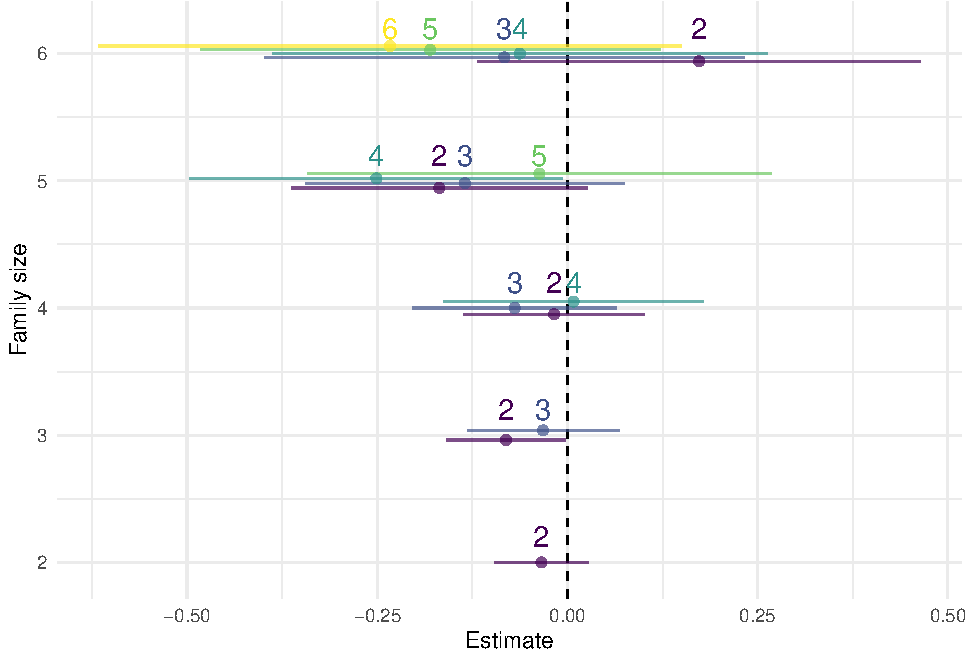
\includegraphics{room-at-the-top_files/figure-latex/pic-bo-psea-interactions-1} 

}

\caption{Regressions of spouse PSEA: birth order dummies within different family sizes. Labels show birth order. Lines are 95 per cent confidence intervals clustered by assessment centre. }\label{fig:pic-bo-psea-interactions}
\end{figure}

 
  \providecommand{\huxb}[2]{\arrayrulecolor[RGB]{#1}\global\arrayrulewidth=#2pt}
  \providecommand{\huxvb}[2]{\color[RGB]{#1}\vrule width #2pt}
  \providecommand{\huxtpad}[1]{\rule{0pt}{#1}}
  \providecommand{\huxbpad}[1]{\rule[-#1]{0pt}{#1}}

\begin{table}[ht]
\begin{centerbox}
\begin{threeparttable}
\captionsetup{justification=centering,singlelinecheck=off}
\caption{\label{tab:tbl-bo-psea-pgs} Regressions of spouse PSEA with controls for polygenic scores}
 \setlength{\tabcolsep}{0pt}
\begin{tabularx}{1\textwidth}{p{0.166666666666667\textwidth} p{0.166666666666667\textwidth} p{0.166666666666667\textwidth} p{0.166666666666667\textwidth} p{0.166666666666667\textwidth} p{0.166666666666667\textwidth}}


\hhline{>{\huxb{0, 0, 0}{0.8}}->{\huxb{0, 0, 0}{0.8}}->{\huxb{0, 0, 0}{0.8}}->{\huxb{0, 0, 0}{0.8}}->{\huxb{0, 0, 0}{0.8}}->{\huxb{0, 0, 0}{0.8}}-}
\arrayrulecolor{black}

\multicolumn{1}{!{\huxvb{0, 0, 0}{0}}p{0.166666666666667\textwidth}!{\huxvb{0, 0, 0}{0}}}{\hspace{6pt}\parbox[b]{0.166666666666667\textwidth-6pt-6pt}{\huxtpad{6pt + 1em}\centering \huxbpad{6pt}}} &
\multicolumn{1}{p{0.166666666666667\textwidth}!{\huxvb{0, 0, 0}{0}}}{\hspace{6pt}\parbox[b]{0.166666666666667\textwidth-6pt-6pt}{\huxtpad{6pt + 1em}\centering (1)\huxbpad{6pt}}} &
\multicolumn{1}{p{0.166666666666667\textwidth}!{\huxvb{0, 0, 0}{0}}}{\hspace{6pt}\parbox[b]{0.166666666666667\textwidth-6pt-6pt}{\huxtpad{6pt + 1em}\centering (2)\huxbpad{6pt}}} &
\multicolumn{1}{p{0.166666666666667\textwidth}!{\huxvb{0, 0, 0}{0}}}{\hspace{6pt}\parbox[b]{0.166666666666667\textwidth-6pt-6pt}{\huxtpad{6pt + 1em}\centering (3)\huxbpad{6pt}}} &
\multicolumn{1}{p{0.166666666666667\textwidth}!{\huxvb{0, 0, 0}{0}}}{\hspace{6pt}\parbox[b]{0.166666666666667\textwidth-6pt-6pt}{\huxtpad{6pt + 1em}\centering (4)\huxbpad{6pt}}} &
\multicolumn{1}{p{0.166666666666667\textwidth}!{\huxvb{0, 0, 0}{0}}}{\hspace{6pt}\parbox[b]{0.166666666666667\textwidth-6pt-6pt}{\huxtpad{6pt + 1em}\centering (5)\huxbpad{6pt}}} \tabularnewline[-0.5pt]


\hhline{>{\huxb{255, 255, 255}{0.4}}->{\huxb{0, 0, 0}{0.4}}->{\huxb{0, 0, 0}{0.4}}->{\huxb{0, 0, 0}{0.4}}->{\huxb{0, 0, 0}{0.4}}->{\huxb{0, 0, 0}{0.4}}-}
\arrayrulecolor{black}

\multicolumn{1}{!{\huxvb{0, 0, 0}{0}}p{0.166666666666667\textwidth}!{\huxvb{0, 0, 0}{0}}}{\hspace{6pt}\parbox[b]{0.166666666666667\textwidth-6pt-6pt}{\huxtpad{6pt + 1em}\raggedright Birth order\huxbpad{6pt}}} &
\multicolumn{1}{p{0.166666666666667\textwidth}!{\huxvb{0, 0, 0}{0}}}{\hspace{6pt}\parbox[b]{0.166666666666667\textwidth-6pt-6pt}{\huxtpad{6pt + 1em}\raggedleft -0.0325 +~\huxbpad{6pt}}} &
\multicolumn{1}{p{0.166666666666667\textwidth}!{\huxvb{0, 0, 0}{0}}}{\hspace{6pt}\parbox[b]{0.166666666666667\textwidth-6pt-6pt}{\huxtpad{6pt + 1em}\raggedleft -0.0177~~~~\huxbpad{6pt}}} &
\multicolumn{1}{p{0.166666666666667\textwidth}!{\huxvb{0, 0, 0}{0}}}{\hspace{6pt}\parbox[b]{0.166666666666667\textwidth-6pt-6pt}{\huxtpad{6pt + 1em}\raggedleft -0.0043~~~~\huxbpad{6pt}}} &
\multicolumn{1}{p{0.166666666666667\textwidth}!{\huxvb{0, 0, 0}{0}}}{\hspace{6pt}\parbox[b]{0.166666666666667\textwidth-6pt-6pt}{\huxtpad{6pt + 1em}\raggedleft 0.0080~~~\huxbpad{6pt}}} &
\multicolumn{1}{p{0.166666666666667\textwidth}!{\huxvb{0, 0, 0}{0}}}{\hspace{6pt}\parbox[b]{0.166666666666667\textwidth-6pt-6pt}{\huxtpad{6pt + 1em}\raggedleft 0.0144~~~\huxbpad{6pt}}} \tabularnewline[-0.5pt]


\hhline{}
\arrayrulecolor{black}

\multicolumn{1}{!{\huxvb{0, 0, 0}{0}}p{0.166666666666667\textwidth}!{\huxvb{0, 0, 0}{0}}}{\hspace{6pt}\parbox[b]{0.166666666666667\textwidth-6pt-6pt}{\huxtpad{6pt + 1em}\raggedright \huxbpad{6pt}}} &
\multicolumn{1}{p{0.166666666666667\textwidth}!{\huxvb{0, 0, 0}{0}}}{\hspace{6pt}\parbox[b]{0.166666666666667\textwidth-6pt-6pt}{\huxtpad{6pt + 1em}\raggedleft (0.0169)~~\huxbpad{6pt}}} &
\multicolumn{1}{p{0.166666666666667\textwidth}!{\huxvb{0, 0, 0}{0}}}{\hspace{6pt}\parbox[b]{0.166666666666667\textwidth-6pt-6pt}{\huxtpad{6pt + 1em}\raggedleft (0.0165)~~~\huxbpad{6pt}}} &
\multicolumn{1}{p{0.166666666666667\textwidth}!{\huxvb{0, 0, 0}{0}}}{\hspace{6pt}\parbox[b]{0.166666666666667\textwidth-6pt-6pt}{\huxtpad{6pt + 1em}\raggedleft (0.0163)~~~\huxbpad{6pt}}} &
\multicolumn{1}{p{0.166666666666667\textwidth}!{\huxvb{0, 0, 0}{0}}}{\hspace{6pt}\parbox[b]{0.166666666666667\textwidth-6pt-6pt}{\huxtpad{6pt + 1em}\raggedleft (0.0357)~~\huxbpad{6pt}}} &
\multicolumn{1}{p{0.166666666666667\textwidth}!{\huxvb{0, 0, 0}{0}}}{\hspace{6pt}\parbox[b]{0.166666666666667\textwidth-6pt-6pt}{\huxtpad{6pt + 1em}\raggedleft (0.0357)~~\huxbpad{6pt}}} \tabularnewline[-0.5pt]


\hhline{}
\arrayrulecolor{black}

\multicolumn{1}{!{\huxvb{0, 0, 0}{0}}p{0.166666666666667\textwidth}!{\huxvb{0, 0, 0}{0}}}{\hspace{6pt}\parbox[b]{0.166666666666667\textwidth-6pt-6pt}{\huxtpad{6pt + 1em}\raggedright University\huxbpad{6pt}}} &
\multicolumn{1}{p{0.166666666666667\textwidth}!{\huxvb{0, 0, 0}{0}}}{\hspace{6pt}\parbox[b]{0.166666666666667\textwidth-6pt-6pt}{\huxtpad{6pt + 1em}\raggedleft ~~~~~~~~\huxbpad{6pt}}} &
\multicolumn{1}{p{0.166666666666667\textwidth}!{\huxvb{0, 0, 0}{0}}}{\hspace{6pt}\parbox[b]{0.166666666666667\textwidth-6pt-6pt}{\huxtpad{6pt + 1em}\raggedleft ~~~~~~~~~\huxbpad{6pt}}} &
\multicolumn{1}{p{0.166666666666667\textwidth}!{\huxvb{0, 0, 0}{0}}}{\hspace{6pt}\parbox[b]{0.166666666666667\textwidth-6pt-6pt}{\huxtpad{6pt + 1em}\raggedleft 0.2280 ***\huxbpad{6pt}}} &
\multicolumn{1}{p{0.166666666666667\textwidth}!{\huxvb{0, 0, 0}{0}}}{\hspace{6pt}\parbox[b]{0.166666666666667\textwidth-6pt-6pt}{\huxtpad{6pt + 1em}\raggedleft ~~~~~~~~\huxbpad{6pt}}} &
\multicolumn{1}{p{0.166666666666667\textwidth}!{\huxvb{0, 0, 0}{0}}}{\hspace{6pt}\parbox[b]{0.166666666666667\textwidth-6pt-6pt}{\huxtpad{6pt + 1em}\raggedleft 0.1405 **\huxbpad{6pt}}} \tabularnewline[-0.5pt]


\hhline{}
\arrayrulecolor{black}

\multicolumn{1}{!{\huxvb{0, 0, 0}{0}}p{0.166666666666667\textwidth}!{\huxvb{0, 0, 0}{0}}}{\hspace{6pt}\parbox[b]{0.166666666666667\textwidth-6pt-6pt}{\huxtpad{6pt + 1em}\raggedright \huxbpad{6pt}}} &
\multicolumn{1}{p{0.166666666666667\textwidth}!{\huxvb{0, 0, 0}{0}}}{\hspace{6pt}\parbox[b]{0.166666666666667\textwidth-6pt-6pt}{\huxtpad{6pt + 1em}\raggedleft ~~~~~~~~\huxbpad{6pt}}} &
\multicolumn{1}{p{0.166666666666667\textwidth}!{\huxvb{0, 0, 0}{0}}}{\hspace{6pt}\parbox[b]{0.166666666666667\textwidth-6pt-6pt}{\huxtpad{6pt + 1em}\raggedleft ~~~~~~~~~\huxbpad{6pt}}} &
\multicolumn{1}{p{0.166666666666667\textwidth}!{\huxvb{0, 0, 0}{0}}}{\hspace{6pt}\parbox[b]{0.166666666666667\textwidth-6pt-6pt}{\huxtpad{6pt + 1em}\raggedleft (0.0303)~~~\huxbpad{6pt}}} &
\multicolumn{1}{p{0.166666666666667\textwidth}!{\huxvb{0, 0, 0}{0}}}{\hspace{6pt}\parbox[b]{0.166666666666667\textwidth-6pt-6pt}{\huxtpad{6pt + 1em}\raggedleft ~~~~~~~~\huxbpad{6pt}}} &
\multicolumn{1}{p{0.166666666666667\textwidth}!{\huxvb{0, 0, 0}{0}}}{\hspace{6pt}\parbox[b]{0.166666666666667\textwidth-6pt-6pt}{\huxtpad{6pt + 1em}\raggedleft (0.0374)~~\huxbpad{6pt}}} \tabularnewline[-0.5pt]


\hhline{}
\arrayrulecolor{black}

\multicolumn{1}{!{\huxvb{0, 0, 0}{0}}p{0.166666666666667\textwidth}!{\huxvb{0, 0, 0}{0}}}{\hspace{6pt}\parbox[b]{0.166666666666667\textwidth-6pt-6pt}{\huxtpad{6pt + 1em}\raggedright Income\huxbpad{6pt}}} &
\multicolumn{1}{p{0.166666666666667\textwidth}!{\huxvb{0, 0, 0}{0}}}{\hspace{6pt}\parbox[b]{0.166666666666667\textwidth-6pt-6pt}{\huxtpad{6pt + 1em}\raggedleft ~~~~~~~~\huxbpad{6pt}}} &
\multicolumn{1}{p{0.166666666666667\textwidth}!{\huxvb{0, 0, 0}{0}}}{\hspace{6pt}\parbox[b]{0.166666666666667\textwidth-6pt-6pt}{\huxtpad{6pt + 1em}\raggedleft ~~~~~~~~~\huxbpad{6pt}}} &
\multicolumn{1}{p{0.166666666666667\textwidth}!{\huxvb{0, 0, 0}{0}}}{\hspace{6pt}\parbox[b]{0.166666666666667\textwidth-6pt-6pt}{\huxtpad{6pt + 1em}\raggedleft ~~~~~~~~~\huxbpad{6pt}}} &
\multicolumn{1}{p{0.166666666666667\textwidth}!{\huxvb{0, 0, 0}{0}}}{\hspace{6pt}\parbox[b]{0.166666666666667\textwidth-6pt-6pt}{\huxtpad{6pt + 1em}\raggedleft 0.0033 **\huxbpad{6pt}}} &
\multicolumn{1}{p{0.166666666666667\textwidth}!{\huxvb{0, 0, 0}{0}}}{\hspace{6pt}\parbox[b]{0.166666666666667\textwidth-6pt-6pt}{\huxtpad{6pt + 1em}\raggedleft 0.0027 **\huxbpad{6pt}}} \tabularnewline[-0.5pt]


\hhline{}
\arrayrulecolor{black}

\multicolumn{1}{!{\huxvb{0, 0, 0}{0}}p{0.166666666666667\textwidth}!{\huxvb{0, 0, 0}{0}}}{\hspace{6pt}\parbox[b]{0.166666666666667\textwidth-6pt-6pt}{\huxtpad{6pt + 1em}\raggedright \huxbpad{6pt}}} &
\multicolumn{1}{p{0.166666666666667\textwidth}!{\huxvb{0, 0, 0}{0}}}{\hspace{6pt}\parbox[b]{0.166666666666667\textwidth-6pt-6pt}{\huxtpad{6pt + 1em}\raggedleft ~~~~~~~~\huxbpad{6pt}}} &
\multicolumn{1}{p{0.166666666666667\textwidth}!{\huxvb{0, 0, 0}{0}}}{\hspace{6pt}\parbox[b]{0.166666666666667\textwidth-6pt-6pt}{\huxtpad{6pt + 1em}\raggedleft ~~~~~~~~~\huxbpad{6pt}}} &
\multicolumn{1}{p{0.166666666666667\textwidth}!{\huxvb{0, 0, 0}{0}}}{\hspace{6pt}\parbox[b]{0.166666666666667\textwidth-6pt-6pt}{\huxtpad{6pt + 1em}\raggedleft ~~~~~~~~~\huxbpad{6pt}}} &
\multicolumn{1}{p{0.166666666666667\textwidth}!{\huxvb{0, 0, 0}{0}}}{\hspace{6pt}\parbox[b]{0.166666666666667\textwidth-6pt-6pt}{\huxtpad{6pt + 1em}\raggedleft (0.0009)~~\huxbpad{6pt}}} &
\multicolumn{1}{p{0.166666666666667\textwidth}!{\huxvb{0, 0, 0}{0}}}{\hspace{6pt}\parbox[b]{0.166666666666667\textwidth-6pt-6pt}{\huxtpad{6pt + 1em}\raggedleft (0.0009)~~\huxbpad{6pt}}} \tabularnewline[-0.5pt]


\hhline{}
\arrayrulecolor{black}

\multicolumn{1}{!{\huxvb{0, 0, 0}{0}}p{0.166666666666667\textwidth}!{\huxvb{0, 0, 0}{0}}}{\hspace{6pt}\parbox[b]{0.166666666666667\textwidth-6pt-6pt}{\huxtpad{6pt + 1em}\raggedright Mother's age at birth\huxbpad{6pt}}} &
\multicolumn{1}{p{0.166666666666667\textwidth}!{\huxvb{0, 0, 0}{0}}}{\hspace{6pt}\parbox[b]{0.166666666666667\textwidth-6pt-6pt}{\huxtpad{6pt + 1em}\raggedleft 0.0099 **\huxbpad{6pt}}} &
\multicolumn{1}{p{0.166666666666667\textwidth}!{\huxvb{0, 0, 0}{0}}}{\hspace{6pt}\parbox[b]{0.166666666666667\textwidth-6pt-6pt}{\huxtpad{6pt + 1em}\raggedleft 0.0070 *~~\huxbpad{6pt}}} &
\multicolumn{1}{p{0.166666666666667\textwidth}!{\huxvb{0, 0, 0}{0}}}{\hspace{6pt}\parbox[b]{0.166666666666667\textwidth-6pt-6pt}{\huxtpad{6pt + 1em}\raggedleft 0.0043~~~~\huxbpad{6pt}}} &
\multicolumn{1}{p{0.166666666666667\textwidth}!{\huxvb{0, 0, 0}{0}}}{\hspace{6pt}\parbox[b]{0.166666666666667\textwidth-6pt-6pt}{\huxtpad{6pt + 1em}\raggedleft 0.0070~~~\huxbpad{6pt}}} &
\multicolumn{1}{p{0.166666666666667\textwidth}!{\huxvb{0, 0, 0}{0}}}{\hspace{6pt}\parbox[b]{0.166666666666667\textwidth-6pt-6pt}{\huxtpad{6pt + 1em}\raggedleft 0.0057~~~\huxbpad{6pt}}} \tabularnewline[-0.5pt]


\hhline{}
\arrayrulecolor{black}

\multicolumn{1}{!{\huxvb{0, 0, 0}{0}}p{0.166666666666667\textwidth}!{\huxvb{0, 0, 0}{0}}}{\hspace{6pt}\parbox[b]{0.166666666666667\textwidth-6pt-6pt}{\huxtpad{6pt + 1em}\raggedright \huxbpad{6pt}}} &
\multicolumn{1}{p{0.166666666666667\textwidth}!{\huxvb{0, 0, 0}{0}}}{\hspace{6pt}\parbox[b]{0.166666666666667\textwidth-6pt-6pt}{\huxtpad{6pt + 1em}\raggedleft (0.0026)~~\huxbpad{6pt}}} &
\multicolumn{1}{p{0.166666666666667\textwidth}!{\huxvb{0, 0, 0}{0}}}{\hspace{6pt}\parbox[b]{0.166666666666667\textwidth-6pt-6pt}{\huxtpad{6pt + 1em}\raggedleft (0.0026)~~~\huxbpad{6pt}}} &
\multicolumn{1}{p{0.166666666666667\textwidth}!{\huxvb{0, 0, 0}{0}}}{\hspace{6pt}\parbox[b]{0.166666666666667\textwidth-6pt-6pt}{\huxtpad{6pt + 1em}\raggedleft (0.0027)~~~\huxbpad{6pt}}} &
\multicolumn{1}{p{0.166666666666667\textwidth}!{\huxvb{0, 0, 0}{0}}}{\hspace{6pt}\parbox[b]{0.166666666666667\textwidth-6pt-6pt}{\huxtpad{6pt + 1em}\raggedleft (0.0052)~~\huxbpad{6pt}}} &
\multicolumn{1}{p{0.166666666666667\textwidth}!{\huxvb{0, 0, 0}{0}}}{\hspace{6pt}\parbox[b]{0.166666666666667\textwidth-6pt-6pt}{\huxtpad{6pt + 1em}\raggedleft (0.0053)~~\huxbpad{6pt}}} \tabularnewline[-0.5pt]


\hhline{}
\arrayrulecolor{black}

\multicolumn{1}{!{\huxvb{0, 0, 0}{0}}p{0.166666666666667\textwidth}!{\huxvb{0, 0, 0}{0}}}{\hspace{6pt}\parbox[b]{0.166666666666667\textwidth-6pt-6pt}{\huxtpad{6pt + 1em}\raggedright Own PSEA\huxbpad{6pt}}} &
\multicolumn{1}{p{0.166666666666667\textwidth}!{\huxvb{0, 0, 0}{0}}}{\hspace{6pt}\parbox[b]{0.166666666666667\textwidth-6pt-6pt}{\huxtpad{6pt + 1em}\raggedleft 0.0528 **\huxbpad{6pt}}} &
\multicolumn{1}{p{0.166666666666667\textwidth}!{\huxvb{0, 0, 0}{0}}}{\hspace{6pt}\parbox[b]{0.166666666666667\textwidth-6pt-6pt}{\huxtpad{6pt + 1em}\raggedleft 0.0437 **~\huxbpad{6pt}}} &
\multicolumn{1}{p{0.166666666666667\textwidth}!{\huxvb{0, 0, 0}{0}}}{\hspace{6pt}\parbox[b]{0.166666666666667\textwidth-6pt-6pt}{\huxtpad{6pt + 1em}\raggedleft 0.0287 +~~\huxbpad{6pt}}} &
\multicolumn{1}{p{0.166666666666667\textwidth}!{\huxvb{0, 0, 0}{0}}}{\hspace{6pt}\parbox[b]{0.166666666666667\textwidth-6pt-6pt}{\huxtpad{6pt + 1em}\raggedleft 0.0307~~~\huxbpad{6pt}}} &
\multicolumn{1}{p{0.166666666666667\textwidth}!{\huxvb{0, 0, 0}{0}}}{\hspace{6pt}\parbox[b]{0.166666666666667\textwidth-6pt-6pt}{\huxtpad{6pt + 1em}\raggedleft 0.0212~~~\huxbpad{6pt}}} \tabularnewline[-0.5pt]


\hhline{}
\arrayrulecolor{black}

\multicolumn{1}{!{\huxvb{0, 0, 0}{0}}p{0.166666666666667\textwidth}!{\huxvb{0, 0, 0}{0}}}{\hspace{6pt}\parbox[b]{0.166666666666667\textwidth-6pt-6pt}{\huxtpad{6pt + 1em}\raggedright \huxbpad{6pt}}} &
\multicolumn{1}{p{0.166666666666667\textwidth}!{\huxvb{0, 0, 0}{0}}}{\hspace{6pt}\parbox[b]{0.166666666666667\textwidth-6pt-6pt}{\huxtpad{6pt + 1em}\raggedleft (0.0140)~~\huxbpad{6pt}}} &
\multicolumn{1}{p{0.166666666666667\textwidth}!{\huxvb{0, 0, 0}{0}}}{\hspace{6pt}\parbox[b]{0.166666666666667\textwidth-6pt-6pt}{\huxtpad{6pt + 1em}\raggedleft (0.0141)~~~\huxbpad{6pt}}} &
\multicolumn{1}{p{0.166666666666667\textwidth}!{\huxvb{0, 0, 0}{0}}}{\hspace{6pt}\parbox[b]{0.166666666666667\textwidth-6pt-6pt}{\huxtpad{6pt + 1em}\raggedleft (0.0148)~~~\huxbpad{6pt}}} &
\multicolumn{1}{p{0.166666666666667\textwidth}!{\huxvb{0, 0, 0}{0}}}{\hspace{6pt}\parbox[b]{0.166666666666667\textwidth-6pt-6pt}{\huxtpad{6pt + 1em}\raggedleft (0.0240)~~\huxbpad{6pt}}} &
\multicolumn{1}{p{0.166666666666667\textwidth}!{\huxvb{0, 0, 0}{0}}}{\hspace{6pt}\parbox[b]{0.166666666666667\textwidth-6pt-6pt}{\huxtpad{6pt + 1em}\raggedleft (0.0238)~~\huxbpad{6pt}}} \tabularnewline[-0.5pt]


\hhline{}
\arrayrulecolor{black}

\multicolumn{1}{!{\huxvb{0, 0, 0}{0}}p{0.166666666666667\textwidth}!{\huxvb{0, 0, 0}{0}}}{\hspace{6pt}\parbox[b]{0.166666666666667\textwidth-6pt-6pt}{\huxtpad{6pt + 1em}\raggedright Fluid IQ\huxbpad{6pt}}} &
\multicolumn{1}{p{0.166666666666667\textwidth}!{\huxvb{0, 0, 0}{0}}}{\hspace{6pt}\parbox[b]{0.166666666666667\textwidth-6pt-6pt}{\huxtpad{6pt + 1em}\raggedleft ~~~~~~~~\huxbpad{6pt}}} &
\multicolumn{1}{p{0.166666666666667\textwidth}!{\huxvb{0, 0, 0}{0}}}{\hspace{6pt}\parbox[b]{0.166666666666667\textwidth-6pt-6pt}{\huxtpad{6pt + 1em}\raggedleft 0.0331 ***\huxbpad{6pt}}} &
\multicolumn{1}{p{0.166666666666667\textwidth}!{\huxvb{0, 0, 0}{0}}}{\hspace{6pt}\parbox[b]{0.166666666666667\textwidth-6pt-6pt}{\huxtpad{6pt + 1em}\raggedleft 0.0174 *~~\huxbpad{6pt}}} &
\multicolumn{1}{p{0.166666666666667\textwidth}!{\huxvb{0, 0, 0}{0}}}{\hspace{6pt}\parbox[b]{0.166666666666667\textwidth-6pt-6pt}{\huxtpad{6pt + 1em}\raggedleft 0.0228 +~\huxbpad{6pt}}} &
\multicolumn{1}{p{0.166666666666667\textwidth}!{\huxvb{0, 0, 0}{0}}}{\hspace{6pt}\parbox[b]{0.166666666666667\textwidth-6pt-6pt}{\huxtpad{6pt + 1em}\raggedleft 0.0147~~~\huxbpad{6pt}}} \tabularnewline[-0.5pt]


\hhline{}
\arrayrulecolor{black}

\multicolumn{1}{!{\huxvb{0, 0, 0}{0}}p{0.166666666666667\textwidth}!{\huxvb{0, 0, 0}{0}}}{\hspace{6pt}\parbox[b]{0.166666666666667\textwidth-6pt-6pt}{\huxtpad{6pt + 1em}\raggedright \huxbpad{6pt}}} &
\multicolumn{1}{p{0.166666666666667\textwidth}!{\huxvb{0, 0, 0}{0}}}{\hspace{6pt}\parbox[b]{0.166666666666667\textwidth-6pt-6pt}{\huxtpad{6pt + 1em}\raggedleft ~~~~~~~~\huxbpad{6pt}}} &
\multicolumn{1}{p{0.166666666666667\textwidth}!{\huxvb{0, 0, 0}{0}}}{\hspace{6pt}\parbox[b]{0.166666666666667\textwidth-6pt-6pt}{\huxtpad{6pt + 1em}\raggedleft (0.0058)~~~\huxbpad{6pt}}} &
\multicolumn{1}{p{0.166666666666667\textwidth}!{\huxvb{0, 0, 0}{0}}}{\hspace{6pt}\parbox[b]{0.166666666666667\textwidth-6pt-6pt}{\huxtpad{6pt + 1em}\raggedleft (0.0070)~~~\huxbpad{6pt}}} &
\multicolumn{1}{p{0.166666666666667\textwidth}!{\huxvb{0, 0, 0}{0}}}{\hspace{6pt}\parbox[b]{0.166666666666667\textwidth-6pt-6pt}{\huxtpad{6pt + 1em}\raggedleft (0.0121)~~\huxbpad{6pt}}} &
\multicolumn{1}{p{0.166666666666667\textwidth}!{\huxvb{0, 0, 0}{0}}}{\hspace{6pt}\parbox[b]{0.166666666666667\textwidth-6pt-6pt}{\huxtpad{6pt + 1em}\raggedleft (0.0129)~~\huxbpad{6pt}}} \tabularnewline[-0.5pt]


\hhline{}
\arrayrulecolor{black}

\multicolumn{1}{!{\huxvb{0, 0, 0}{0}}p{0.166666666666667\textwidth}!{\huxvb{0, 0, 0}{0}}}{\hspace{6pt}\parbox[b]{0.166666666666667\textwidth-6pt-6pt}{\huxtpad{6pt + 1em}\raggedright Height\huxbpad{6pt}}} &
\multicolumn{1}{p{0.166666666666667\textwidth}!{\huxvb{0, 0, 0}{0}}}{\hspace{6pt}\parbox[b]{0.166666666666667\textwidth-6pt-6pt}{\huxtpad{6pt + 1em}\raggedleft ~~~~~~~~\huxbpad{6pt}}} &
\multicolumn{1}{p{0.166666666666667\textwidth}!{\huxvb{0, 0, 0}{0}}}{\hspace{6pt}\parbox[b]{0.166666666666667\textwidth-6pt-6pt}{\huxtpad{6pt + 1em}\raggedleft 0.0030 *~~\huxbpad{6pt}}} &
\multicolumn{1}{p{0.166666666666667\textwidth}!{\huxvb{0, 0, 0}{0}}}{\hspace{6pt}\parbox[b]{0.166666666666667\textwidth-6pt-6pt}{\huxtpad{6pt + 1em}\raggedleft 0.0023 +~~\huxbpad{6pt}}} &
\multicolumn{1}{p{0.166666666666667\textwidth}!{\huxvb{0, 0, 0}{0}}}{\hspace{6pt}\parbox[b]{0.166666666666667\textwidth-6pt-6pt}{\huxtpad{6pt + 1em}\raggedleft 0.0050 +~\huxbpad{6pt}}} &
\multicolumn{1}{p{0.166666666666667\textwidth}!{\huxvb{0, 0, 0}{0}}}{\hspace{6pt}\parbox[b]{0.166666666666667\textwidth-6pt-6pt}{\huxtpad{6pt + 1em}\raggedleft 0.0047 +~\huxbpad{6pt}}} \tabularnewline[-0.5pt]


\hhline{}
\arrayrulecolor{black}

\multicolumn{1}{!{\huxvb{0, 0, 0}{0}}p{0.166666666666667\textwidth}!{\huxvb{0, 0, 0}{0}}}{\hspace{6pt}\parbox[b]{0.166666666666667\textwidth-6pt-6pt}{\huxtpad{6pt + 1em}\raggedright \huxbpad{6pt}}} &
\multicolumn{1}{p{0.166666666666667\textwidth}!{\huxvb{0, 0, 0}{0}}}{\hspace{6pt}\parbox[b]{0.166666666666667\textwidth-6pt-6pt}{\huxtpad{6pt + 1em}\raggedleft ~~~~~~~~\huxbpad{6pt}}} &
\multicolumn{1}{p{0.166666666666667\textwidth}!{\huxvb{0, 0, 0}{0}}}{\hspace{6pt}\parbox[b]{0.166666666666667\textwidth-6pt-6pt}{\huxtpad{6pt + 1em}\raggedleft (0.0013)~~~\huxbpad{6pt}}} &
\multicolumn{1}{p{0.166666666666667\textwidth}!{\huxvb{0, 0, 0}{0}}}{\hspace{6pt}\parbox[b]{0.166666666666667\textwidth-6pt-6pt}{\huxtpad{6pt + 1em}\raggedleft (0.0013)~~~\huxbpad{6pt}}} &
\multicolumn{1}{p{0.166666666666667\textwidth}!{\huxvb{0, 0, 0}{0}}}{\hspace{6pt}\parbox[b]{0.166666666666667\textwidth-6pt-6pt}{\huxtpad{6pt + 1em}\raggedleft (0.0027)~~\huxbpad{6pt}}} &
\multicolumn{1}{p{0.166666666666667\textwidth}!{\huxvb{0, 0, 0}{0}}}{\hspace{6pt}\parbox[b]{0.166666666666667\textwidth-6pt-6pt}{\huxtpad{6pt + 1em}\raggedleft (0.0027)~~\huxbpad{6pt}}} \tabularnewline[-0.5pt]


\hhline{>{\huxb{255, 255, 255}{0.4}}->{\huxb{0, 0, 0}{0.4}}->{\huxb{0, 0, 0}{0.4}}->{\huxb{0, 0, 0}{0.4}}->{\huxb{0, 0, 0}{0.4}}->{\huxb{0, 0, 0}{0.4}}-}
\arrayrulecolor{black}

\multicolumn{1}{!{\huxvb{0, 0, 0}{0}}p{0.166666666666667\textwidth}!{\huxvb{0, 0, 0}{0}}}{\hspace{6pt}\parbox[b]{0.166666666666667\textwidth-6pt-6pt}{\huxtpad{6pt + 1em}\raggedright Family size dummies\huxbpad{6pt}}} &
\multicolumn{1}{p{0.166666666666667\textwidth}!{\huxvb{0, 0, 0}{0}}}{\hspace{6pt}\parbox[b]{0.166666666666667\textwidth-6pt-6pt}{\huxtpad{6pt + 1em}\raggedleft Yes~~~~~~~~\huxbpad{6pt}}} &
\multicolumn{1}{p{0.166666666666667\textwidth}!{\huxvb{0, 0, 0}{0}}}{\hspace{6pt}\parbox[b]{0.166666666666667\textwidth-6pt-6pt}{\huxtpad{6pt + 1em}\raggedleft Yes~~~~~~~~~\huxbpad{6pt}}} &
\multicolumn{1}{p{0.166666666666667\textwidth}!{\huxvb{0, 0, 0}{0}}}{\hspace{6pt}\parbox[b]{0.166666666666667\textwidth-6pt-6pt}{\huxtpad{6pt + 1em}\raggedleft Yes~~~~~~~~~\huxbpad{6pt}}} &
\multicolumn{1}{p{0.166666666666667\textwidth}!{\huxvb{0, 0, 0}{0}}}{\hspace{6pt}\parbox[b]{0.166666666666667\textwidth-6pt-6pt}{\huxtpad{6pt + 1em}\raggedleft Yes~~~~~~~~\huxbpad{6pt}}} &
\multicolumn{1}{p{0.166666666666667\textwidth}!{\huxvb{0, 0, 0}{0}}}{\hspace{6pt}\parbox[b]{0.166666666666667\textwidth-6pt-6pt}{\huxtpad{6pt + 1em}\raggedleft Yes~~~~~~~~\huxbpad{6pt}}} \tabularnewline[-0.5pt]


\hhline{}
\arrayrulecolor{black}

\multicolumn{1}{!{\huxvb{0, 0, 0}{0}}p{0.166666666666667\textwidth}!{\huxvb{0, 0, 0}{0}}}{\hspace{6pt}\parbox[b]{0.166666666666667\textwidth-6pt-6pt}{\huxtpad{6pt + 1em}\raggedright Birth month dummies\huxbpad{6pt}}} &
\multicolumn{1}{p{0.166666666666667\textwidth}!{\huxvb{0, 0, 0}{0}}}{\hspace{6pt}\parbox[b]{0.166666666666667\textwidth-6pt-6pt}{\huxtpad{6pt + 1em}\raggedleft Yes~~~~~~~~\huxbpad{6pt}}} &
\multicolumn{1}{p{0.166666666666667\textwidth}!{\huxvb{0, 0, 0}{0}}}{\hspace{6pt}\parbox[b]{0.166666666666667\textwidth-6pt-6pt}{\huxtpad{6pt + 1em}\raggedleft Yes~~~~~~~~~\huxbpad{6pt}}} &
\multicolumn{1}{p{0.166666666666667\textwidth}!{\huxvb{0, 0, 0}{0}}}{\hspace{6pt}\parbox[b]{0.166666666666667\textwidth-6pt-6pt}{\huxtpad{6pt + 1em}\raggedleft Yes~~~~~~~~~\huxbpad{6pt}}} &
\multicolumn{1}{p{0.166666666666667\textwidth}!{\huxvb{0, 0, 0}{0}}}{\hspace{6pt}\parbox[b]{0.166666666666667\textwidth-6pt-6pt}{\huxtpad{6pt + 1em}\raggedleft Yes~~~~~~~~\huxbpad{6pt}}} &
\multicolumn{1}{p{0.166666666666667\textwidth}!{\huxvb{0, 0, 0}{0}}}{\hspace{6pt}\parbox[b]{0.166666666666667\textwidth-6pt-6pt}{\huxtpad{6pt + 1em}\raggedleft Yes~~~~~~~~\huxbpad{6pt}}} \tabularnewline[-0.5pt]


\hhline{}
\arrayrulecolor{black}

\multicolumn{1}{!{\huxvb{0, 0, 0}{0}}p{0.166666666666667\textwidth}!{\huxvb{0, 0, 0}{0}}}{\hspace{6pt}\parbox[b]{0.166666666666667\textwidth-6pt-6pt}{\huxtpad{6pt + 1em}\raggedright Birth year dummies\huxbpad{6pt}}} &
\multicolumn{1}{p{0.166666666666667\textwidth}!{\huxvb{0, 0, 0}{0}}}{\hspace{6pt}\parbox[b]{0.166666666666667\textwidth-6pt-6pt}{\huxtpad{6pt + 1em}\raggedleft Yes~~~~~~~~\huxbpad{6pt}}} &
\multicolumn{1}{p{0.166666666666667\textwidth}!{\huxvb{0, 0, 0}{0}}}{\hspace{6pt}\parbox[b]{0.166666666666667\textwidth-6pt-6pt}{\huxtpad{6pt + 1em}\raggedleft Yes~~~~~~~~~\huxbpad{6pt}}} &
\multicolumn{1}{p{0.166666666666667\textwidth}!{\huxvb{0, 0, 0}{0}}}{\hspace{6pt}\parbox[b]{0.166666666666667\textwidth-6pt-6pt}{\huxtpad{6pt + 1em}\raggedleft Yes~~~~~~~~~\huxbpad{6pt}}} &
\multicolumn{1}{p{0.166666666666667\textwidth}!{\huxvb{0, 0, 0}{0}}}{\hspace{6pt}\parbox[b]{0.166666666666667\textwidth-6pt-6pt}{\huxtpad{6pt + 1em}\raggedleft Yes~~~~~~~~\huxbpad{6pt}}} &
\multicolumn{1}{p{0.166666666666667\textwidth}!{\huxvb{0, 0, 0}{0}}}{\hspace{6pt}\parbox[b]{0.166666666666667\textwidth-6pt-6pt}{\huxtpad{6pt + 1em}\raggedleft Yes~~~~~~~~\huxbpad{6pt}}} \tabularnewline[-0.5pt]


\hhline{}
\arrayrulecolor{black}

\multicolumn{1}{!{\huxvb{0, 0, 0}{0}}p{0.166666666666667\textwidth}!{\huxvb{0, 0, 0}{0}}}{\hspace{6pt}\parbox[b]{0.166666666666667\textwidth-6pt-6pt}{\huxtpad{6pt + 1em}\raggedright Polygenic score controls\huxbpad{6pt}}} &
\multicolumn{1}{p{0.166666666666667\textwidth}!{\huxvb{0, 0, 0}{0}}}{\hspace{6pt}\parbox[b]{0.166666666666667\textwidth-6pt-6pt}{\huxtpad{6pt + 1em}\raggedleft Yes~~~~~~~~\huxbpad{6pt}}} &
\multicolumn{1}{p{0.166666666666667\textwidth}!{\huxvb{0, 0, 0}{0}}}{\hspace{6pt}\parbox[b]{0.166666666666667\textwidth-6pt-6pt}{\huxtpad{6pt + 1em}\raggedleft Yes~~~~~~~~~\huxbpad{6pt}}} &
\multicolumn{1}{p{0.166666666666667\textwidth}!{\huxvb{0, 0, 0}{0}}}{\hspace{6pt}\parbox[b]{0.166666666666667\textwidth-6pt-6pt}{\huxtpad{6pt + 1em}\raggedleft Yes~~~~~~~~~\huxbpad{6pt}}} &
\multicolumn{1}{p{0.166666666666667\textwidth}!{\huxvb{0, 0, 0}{0}}}{\hspace{6pt}\parbox[b]{0.166666666666667\textwidth-6pt-6pt}{\huxtpad{6pt + 1em}\raggedleft Yes~~~~~~~~\huxbpad{6pt}}} &
\multicolumn{1}{p{0.166666666666667\textwidth}!{\huxvb{0, 0, 0}{0}}}{\hspace{6pt}\parbox[b]{0.166666666666667\textwidth-6pt-6pt}{\huxtpad{6pt + 1em}\raggedleft Yes~~~~~~~~\huxbpad{6pt}}} \tabularnewline[-0.5pt]


\hhline{>{\huxb{255, 255, 255}{0.4}}->{\huxb{0, 0, 0}{0.4}}->{\huxb{0, 0, 0}{0.4}}->{\huxb{0, 0, 0}{0.4}}->{\huxb{0, 0, 0}{0.4}}->{\huxb{0, 0, 0}{0.4}}-}
\arrayrulecolor{black}

\multicolumn{1}{!{\huxvb{0, 0, 0}{0}}p{0.166666666666667\textwidth}!{\huxvb{0, 0, 0}{0}}}{\hspace{6pt}\parbox[b]{0.166666666666667\textwidth-6pt-6pt}{\huxtpad{6pt + 1em}\raggedright N\huxbpad{6pt}}} &
\multicolumn{1}{p{0.166666666666667\textwidth}!{\huxvb{0, 0, 0}{0}}}{\hspace{6pt}\parbox[b]{0.166666666666667\textwidth-6pt-6pt}{\huxtpad{6pt + 1em}\raggedleft 8970~~~~~~~~\huxbpad{6pt}}} &
\multicolumn{1}{p{0.166666666666667\textwidth}!{\huxvb{0, 0, 0}{0}}}{\hspace{6pt}\parbox[b]{0.166666666666667\textwidth-6pt-6pt}{\huxtpad{6pt + 1em}\raggedleft 8780~~~~~~~~~\huxbpad{6pt}}} &
\multicolumn{1}{p{0.166666666666667\textwidth}!{\huxvb{0, 0, 0}{0}}}{\hspace{6pt}\parbox[b]{0.166666666666667\textwidth-6pt-6pt}{\huxtpad{6pt + 1em}\raggedleft 8778~~~~~~~~~\huxbpad{6pt}}} &
\multicolumn{1}{p{0.166666666666667\textwidth}!{\huxvb{0, 0, 0}{0}}}{\hspace{6pt}\parbox[b]{0.166666666666667\textwidth-6pt-6pt}{\huxtpad{6pt + 1em}\raggedleft 2920~~~~~~~~\huxbpad{6pt}}} &
\multicolumn{1}{p{0.166666666666667\textwidth}!{\huxvb{0, 0, 0}{0}}}{\hspace{6pt}\parbox[b]{0.166666666666667\textwidth-6pt-6pt}{\huxtpad{6pt + 1em}\raggedleft 2919~~~~~~~~\huxbpad{6pt}}} \tabularnewline[-0.5pt]


\hhline{}
\arrayrulecolor{black}

\multicolumn{1}{!{\huxvb{0, 0, 0}{0}}p{0.166666666666667\textwidth}!{\huxvb{0, 0, 0}{0}}}{\hspace{6pt}\parbox[b]{0.166666666666667\textwidth-6pt-6pt}{\huxtpad{6pt + 1em}\raggedright R2\huxbpad{6pt}}} &
\multicolumn{1}{p{0.166666666666667\textwidth}!{\huxvb{0, 0, 0}{0}}}{\hspace{6pt}\parbox[b]{0.166666666666667\textwidth-6pt-6pt}{\huxtpad{6pt + 1em}\raggedleft 0.014~~~~\huxbpad{6pt}}} &
\multicolumn{1}{p{0.166666666666667\textwidth}!{\huxvb{0, 0, 0}{0}}}{\hspace{6pt}\parbox[b]{0.166666666666667\textwidth-6pt-6pt}{\huxtpad{6pt + 1em}\raggedleft 0.020~~~~~\huxbpad{6pt}}} &
\multicolumn{1}{p{0.166666666666667\textwidth}!{\huxvb{0, 0, 0}{0}}}{\hspace{6pt}\parbox[b]{0.166666666666667\textwidth-6pt-6pt}{\huxtpad{6pt + 1em}\raggedleft 0.030~~~~~\huxbpad{6pt}}} &
\multicolumn{1}{p{0.166666666666667\textwidth}!{\huxvb{0, 0, 0}{0}}}{\hspace{6pt}\parbox[b]{0.166666666666667\textwidth-6pt-6pt}{\huxtpad{6pt + 1em}\raggedleft 0.034~~~~\huxbpad{6pt}}} &
\multicolumn{1}{p{0.166666666666667\textwidth}!{\huxvb{0, 0, 0}{0}}}{\hspace{6pt}\parbox[b]{0.166666666666667\textwidth-6pt-6pt}{\huxtpad{6pt + 1em}\raggedleft 0.038~~~~\huxbpad{6pt}}} \tabularnewline[-0.5pt]


\hhline{>{\huxb{0, 0, 0}{0.8}}->{\huxb{0, 0, 0}{0.8}}->{\huxb{0, 0, 0}{0.8}}->{\huxb{0, 0, 0}{0.8}}->{\huxb{0, 0, 0}{0.8}}->{\huxb{0, 0, 0}{0.8}}-}
\arrayrulecolor{black}

\multicolumn{6}{!{\huxvb{0, 0, 0}{0}}p{1\textwidth+10\tabcolsep}!{\huxvb{0, 0, 0}{0}}}{\hspace{6pt}\parbox[b]{1\textwidth+10\tabcolsep-6pt-6pt}{\huxtpad{6pt + 1em}\raggedright  *** p $<$ 0.001;  ** p $<$ 0.01;  * p $<$ 0.05;  + p $<$ 0.1. Standard errors: robust.  \newline Polygenic scores: alzheimer's, caffeine, cognitive ability, neuroticism, substance use.\huxbpad{6pt}}} \tabularnewline[-0.5pt]


\hhline{}
\arrayrulecolor{black}
\end{tabularx}
\end{threeparttable}\par\end{centerbox}

\end{table}
 

 
  \providecommand{\huxb}[2]{\arrayrulecolor[RGB]{#1}\global\arrayrulewidth=#2pt}
  \providecommand{\huxvb}[2]{\color[RGB]{#1}\vrule width #2pt}
  \providecommand{\huxtpad}[1]{\rule{0pt}{#1}}
  \providecommand{\huxbpad}[1]{\rule[-#1]{0pt}{#1}}

\begin{table}[ht]
\begin{centerbox}
\begin{threeparttable}
\captionsetup{justification=centering,singlelinecheck=off}
\caption{\label{tab:tbl-bo-psea-age-fte} Regressions of spouse PSEA using age of leaving full-time education}
 \setlength{\tabcolsep}{0pt}
\begin{tabularx}{0.8\textwidth}{p{0.2\textwidth} p{0.2\textwidth} p{0.2\textwidth} p{0.2\textwidth}}


\hhline{>{\huxb{0, 0, 0}{0.8}}->{\huxb{0, 0, 0}{0.8}}->{\huxb{0, 0, 0}{0.8}}->{\huxb{0, 0, 0}{0.8}}-}
\arrayrulecolor{black}

\multicolumn{1}{!{\huxvb{0, 0, 0}{0}}p{0.2\textwidth}!{\huxvb{0, 0, 0}{0}}}{\hspace{6pt}\parbox[b]{0.2\textwidth-6pt-6pt}{\huxtpad{6pt + 1em}\centering \huxbpad{6pt}}} &
\multicolumn{1}{p{0.2\textwidth}!{\huxvb{0, 0, 0}{0}}}{\hspace{6pt}\parbox[b]{0.2\textwidth-6pt-6pt}{\huxtpad{6pt + 1em}\centering (1)\huxbpad{6pt}}} &
\multicolumn{1}{p{0.2\textwidth}!{\huxvb{0, 0, 0}{0}}}{\hspace{6pt}\parbox[b]{0.2\textwidth-6pt-6pt}{\huxtpad{6pt + 1em}\centering (2)\huxbpad{6pt}}} &
\multicolumn{1}{p{0.2\textwidth}!{\huxvb{0, 0, 0}{0}}}{\hspace{6pt}\parbox[b]{0.2\textwidth-6pt-6pt}{\huxtpad{6pt + 1em}\centering (3)\huxbpad{6pt}}} \tabularnewline[-0.5pt]


\hhline{>{\huxb{255, 255, 255}{0.4}}->{\huxb{0, 0, 0}{0.4}}->{\huxb{0, 0, 0}{0.4}}->{\huxb{0, 0, 0}{0.4}}-}
\arrayrulecolor{black}

\multicolumn{1}{!{\huxvb{0, 0, 0}{0}}p{0.2\textwidth}!{\huxvb{0, 0, 0}{0}}}{\hspace{6pt}\parbox[b]{0.2\textwidth-6pt-6pt}{\huxtpad{6pt + 1em}\raggedright Birth order\huxbpad{6pt}}} &
\multicolumn{1}{p{0.2\textwidth}!{\huxvb{0, 0, 0}{0}}}{\hspace{6pt}\parbox[b]{0.2\textwidth-6pt-6pt}{\huxtpad{6pt + 1em}\raggedleft -0.0173~~~~\huxbpad{6pt}}} &
\multicolumn{1}{p{0.2\textwidth}!{\huxvb{0, 0, 0}{0}}}{\hspace{6pt}\parbox[b]{0.2\textwidth-6pt-6pt}{\huxtpad{6pt + 1em}\raggedleft 0.0016~~~~\huxbpad{6pt}}} &
\multicolumn{1}{p{0.2\textwidth}!{\huxvb{0, 0, 0}{0}}}{\hspace{6pt}\parbox[b]{0.2\textwidth-6pt-6pt}{\huxtpad{6pt + 1em}\raggedleft 0.0223~~~~\huxbpad{6pt}}} \tabularnewline[-0.5pt]


\hhline{}
\arrayrulecolor{black}

\multicolumn{1}{!{\huxvb{0, 0, 0}{0}}p{0.2\textwidth}!{\huxvb{0, 0, 0}{0}}}{\hspace{6pt}\parbox[b]{0.2\textwidth-6pt-6pt}{\huxtpad{6pt + 1em}\raggedright \huxbpad{6pt}}} &
\multicolumn{1}{p{0.2\textwidth}!{\huxvb{0, 0, 0}{0}}}{\hspace{6pt}\parbox[b]{0.2\textwidth-6pt-6pt}{\huxtpad{6pt + 1em}\raggedleft (0.0160)~~~\huxbpad{6pt}}} &
\multicolumn{1}{p{0.2\textwidth}!{\huxvb{0, 0, 0}{0}}}{\hspace{6pt}\parbox[b]{0.2\textwidth-6pt-6pt}{\huxtpad{6pt + 1em}\raggedleft (0.0161)~~~\huxbpad{6pt}}} &
\multicolumn{1}{p{0.2\textwidth}!{\huxvb{0, 0, 0}{0}}}{\hspace{6pt}\parbox[b]{0.2\textwidth-6pt-6pt}{\huxtpad{6pt + 1em}\raggedleft (0.0296)~~~\huxbpad{6pt}}} \tabularnewline[-0.5pt]


\hhline{}
\arrayrulecolor{black}

\multicolumn{1}{!{\huxvb{0, 0, 0}{0}}p{0.2\textwidth}!{\huxvb{0, 0, 0}{0}}}{\hspace{6pt}\parbox[b]{0.2\textwidth-6pt-6pt}{\huxtpad{6pt + 1em}\raggedright Age left full-time educ.\huxbpad{6pt}}} &
\multicolumn{1}{p{0.2\textwidth}!{\huxvb{0, 0, 0}{0}}}{\hspace{6pt}\parbox[b]{0.2\textwidth-6pt-6pt}{\huxtpad{6pt + 1em}\raggedleft ~~~~~~~~~\huxbpad{6pt}}} &
\multicolumn{1}{p{0.2\textwidth}!{\huxvb{0, 0, 0}{0}}}{\hspace{6pt}\parbox[b]{0.2\textwidth-6pt-6pt}{\huxtpad{6pt + 1em}\raggedleft 0.0496 ***\huxbpad{6pt}}} &
\multicolumn{1}{p{0.2\textwidth}!{\huxvb{0, 0, 0}{0}}}{\hspace{6pt}\parbox[b]{0.2\textwidth-6pt-6pt}{\huxtpad{6pt + 1em}\raggedleft 0.0403 ***\huxbpad{6pt}}} \tabularnewline[-0.5pt]


\hhline{}
\arrayrulecolor{black}

\multicolumn{1}{!{\huxvb{0, 0, 0}{0}}p{0.2\textwidth}!{\huxvb{0, 0, 0}{0}}}{\hspace{6pt}\parbox[b]{0.2\textwidth-6pt-6pt}{\huxtpad{6pt + 1em}\raggedright \huxbpad{6pt}}} &
\multicolumn{1}{p{0.2\textwidth}!{\huxvb{0, 0, 0}{0}}}{\hspace{6pt}\parbox[b]{0.2\textwidth-6pt-6pt}{\huxtpad{6pt + 1em}\raggedleft ~~~~~~~~~\huxbpad{6pt}}} &
\multicolumn{1}{p{0.2\textwidth}!{\huxvb{0, 0, 0}{0}}}{\hspace{6pt}\parbox[b]{0.2\textwidth-6pt-6pt}{\huxtpad{6pt + 1em}\raggedleft (0.0047)~~~\huxbpad{6pt}}} &
\multicolumn{1}{p{0.2\textwidth}!{\huxvb{0, 0, 0}{0}}}{\hspace{6pt}\parbox[b]{0.2\textwidth-6pt-6pt}{\huxtpad{6pt + 1em}\raggedleft (0.0083)~~~\huxbpad{6pt}}} \tabularnewline[-0.5pt]


\hhline{}
\arrayrulecolor{black}

\multicolumn{1}{!{\huxvb{0, 0, 0}{0}}p{0.2\textwidth}!{\huxvb{0, 0, 0}{0}}}{\hspace{6pt}\parbox[b]{0.2\textwidth-6pt-6pt}{\huxtpad{6pt + 1em}\raggedright Income\huxbpad{6pt}}} &
\multicolumn{1}{p{0.2\textwidth}!{\huxvb{0, 0, 0}{0}}}{\hspace{6pt}\parbox[b]{0.2\textwidth-6pt-6pt}{\huxtpad{6pt + 1em}\raggedleft ~~~~~~~~~\huxbpad{6pt}}} &
\multicolumn{1}{p{0.2\textwidth}!{\huxvb{0, 0, 0}{0}}}{\hspace{6pt}\parbox[b]{0.2\textwidth-6pt-6pt}{\huxtpad{6pt + 1em}\raggedleft ~~~~~~~~~\huxbpad{6pt}}} &
\multicolumn{1}{p{0.2\textwidth}!{\huxvb{0, 0, 0}{0}}}{\hspace{6pt}\parbox[b]{0.2\textwidth-6pt-6pt}{\huxtpad{6pt + 1em}\raggedleft 0.0025 *~~\huxbpad{6pt}}} \tabularnewline[-0.5pt]


\hhline{}
\arrayrulecolor{black}

\multicolumn{1}{!{\huxvb{0, 0, 0}{0}}p{0.2\textwidth}!{\huxvb{0, 0, 0}{0}}}{\hspace{6pt}\parbox[b]{0.2\textwidth-6pt-6pt}{\huxtpad{6pt + 1em}\raggedright \huxbpad{6pt}}} &
\multicolumn{1}{p{0.2\textwidth}!{\huxvb{0, 0, 0}{0}}}{\hspace{6pt}\parbox[b]{0.2\textwidth-6pt-6pt}{\huxtpad{6pt + 1em}\raggedleft ~~~~~~~~~\huxbpad{6pt}}} &
\multicolumn{1}{p{0.2\textwidth}!{\huxvb{0, 0, 0}{0}}}{\hspace{6pt}\parbox[b]{0.2\textwidth-6pt-6pt}{\huxtpad{6pt + 1em}\raggedleft ~~~~~~~~~\huxbpad{6pt}}} &
\multicolumn{1}{p{0.2\textwidth}!{\huxvb{0, 0, 0}{0}}}{\hspace{6pt}\parbox[b]{0.2\textwidth-6pt-6pt}{\huxtpad{6pt + 1em}\raggedleft (0.0012)~~~\huxbpad{6pt}}} \tabularnewline[-0.5pt]


\hhline{}
\arrayrulecolor{black}

\multicolumn{1}{!{\huxvb{0, 0, 0}{0}}p{0.2\textwidth}!{\huxvb{0, 0, 0}{0}}}{\hspace{6pt}\parbox[b]{0.2\textwidth-6pt-6pt}{\huxtpad{6pt + 1em}\raggedright Mother's age at birth\huxbpad{6pt}}} &
\multicolumn{1}{p{0.2\textwidth}!{\huxvb{0, 0, 0}{0}}}{\hspace{6pt}\parbox[b]{0.2\textwidth-6pt-6pt}{\huxtpad{6pt + 1em}\raggedleft 0.0072 *~~\huxbpad{6pt}}} &
\multicolumn{1}{p{0.2\textwidth}!{\huxvb{0, 0, 0}{0}}}{\hspace{6pt}\parbox[b]{0.2\textwidth-6pt-6pt}{\huxtpad{6pt + 1em}\raggedleft 0.0034~~~~\huxbpad{6pt}}} &
\multicolumn{1}{p{0.2\textwidth}!{\huxvb{0, 0, 0}{0}}}{\hspace{6pt}\parbox[b]{0.2\textwidth-6pt-6pt}{\huxtpad{6pt + 1em}\raggedleft 0.0041~~~~\huxbpad{6pt}}} \tabularnewline[-0.5pt]


\hhline{}
\arrayrulecolor{black}

\multicolumn{1}{!{\huxvb{0, 0, 0}{0}}p{0.2\textwidth}!{\huxvb{0, 0, 0}{0}}}{\hspace{6pt}\parbox[b]{0.2\textwidth-6pt-6pt}{\huxtpad{6pt + 1em}\raggedright \huxbpad{6pt}}} &
\multicolumn{1}{p{0.2\textwidth}!{\huxvb{0, 0, 0}{0}}}{\hspace{6pt}\parbox[b]{0.2\textwidth-6pt-6pt}{\huxtpad{6pt + 1em}\raggedleft (0.0028)~~~\huxbpad{6pt}}} &
\multicolumn{1}{p{0.2\textwidth}!{\huxvb{0, 0, 0}{0}}}{\hspace{6pt}\parbox[b]{0.2\textwidth-6pt-6pt}{\huxtpad{6pt + 1em}\raggedleft (0.0028)~~~\huxbpad{6pt}}} &
\multicolumn{1}{p{0.2\textwidth}!{\huxvb{0, 0, 0}{0}}}{\hspace{6pt}\parbox[b]{0.2\textwidth-6pt-6pt}{\huxtpad{6pt + 1em}\raggedleft (0.0050)~~~\huxbpad{6pt}}} \tabularnewline[-0.5pt]


\hhline{}
\arrayrulecolor{black}

\multicolumn{1}{!{\huxvb{0, 0, 0}{0}}p{0.2\textwidth}!{\huxvb{0, 0, 0}{0}}}{\hspace{6pt}\parbox[b]{0.2\textwidth-6pt-6pt}{\huxtpad{6pt + 1em}\raggedright Own PSEA\huxbpad{6pt}}} &
\multicolumn{1}{p{0.2\textwidth}!{\huxvb{0, 0, 0}{0}}}{\hspace{6pt}\parbox[b]{0.2\textwidth-6pt-6pt}{\huxtpad{6pt + 1em}\raggedleft 0.0491 ***\huxbpad{6pt}}} &
\multicolumn{1}{p{0.2\textwidth}!{\huxvb{0, 0, 0}{0}}}{\hspace{6pt}\parbox[b]{0.2\textwidth-6pt-6pt}{\huxtpad{6pt + 1em}\raggedleft 0.0319 **~\huxbpad{6pt}}} &
\multicolumn{1}{p{0.2\textwidth}!{\huxvb{0, 0, 0}{0}}}{\hspace{6pt}\parbox[b]{0.2\textwidth-6pt-6pt}{\huxtpad{6pt + 1em}\raggedleft 0.0253~~~~\huxbpad{6pt}}} \tabularnewline[-0.5pt]


\hhline{}
\arrayrulecolor{black}

\multicolumn{1}{!{\huxvb{0, 0, 0}{0}}p{0.2\textwidth}!{\huxvb{0, 0, 0}{0}}}{\hspace{6pt}\parbox[b]{0.2\textwidth-6pt-6pt}{\huxtpad{6pt + 1em}\raggedright \huxbpad{6pt}}} &
\multicolumn{1}{p{0.2\textwidth}!{\huxvb{0, 0, 0}{0}}}{\hspace{6pt}\parbox[b]{0.2\textwidth-6pt-6pt}{\huxtpad{6pt + 1em}\raggedleft (0.0109)~~~\huxbpad{6pt}}} &
\multicolumn{1}{p{0.2\textwidth}!{\huxvb{0, 0, 0}{0}}}{\hspace{6pt}\parbox[b]{0.2\textwidth-6pt-6pt}{\huxtpad{6pt + 1em}\raggedleft (0.0110)~~~\huxbpad{6pt}}} &
\multicolumn{1}{p{0.2\textwidth}!{\huxvb{0, 0, 0}{0}}}{\hspace{6pt}\parbox[b]{0.2\textwidth-6pt-6pt}{\huxtpad{6pt + 1em}\raggedleft (0.0205)~~~\huxbpad{6pt}}} \tabularnewline[-0.5pt]


\hhline{}
\arrayrulecolor{black}

\multicolumn{1}{!{\huxvb{0, 0, 0}{0}}p{0.2\textwidth}!{\huxvb{0, 0, 0}{0}}}{\hspace{6pt}\parbox[b]{0.2\textwidth-6pt-6pt}{\huxtpad{6pt + 1em}\raggedright Fluid IQ\huxbpad{6pt}}} &
\multicolumn{1}{p{0.2\textwidth}!{\huxvb{0, 0, 0}{0}}}{\hspace{6pt}\parbox[b]{0.2\textwidth-6pt-6pt}{\huxtpad{6pt + 1em}\raggedleft 0.0337 ***\huxbpad{6pt}}} &
\multicolumn{1}{p{0.2\textwidth}!{\huxvb{0, 0, 0}{0}}}{\hspace{6pt}\parbox[b]{0.2\textwidth-6pt-6pt}{\huxtpad{6pt + 1em}\raggedleft 0.0149 **~\huxbpad{6pt}}} &
\multicolumn{1}{p{0.2\textwidth}!{\huxvb{0, 0, 0}{0}}}{\hspace{6pt}\parbox[b]{0.2\textwidth-6pt-6pt}{\huxtpad{6pt + 1em}\raggedleft 0.0104~~~~\huxbpad{6pt}}} \tabularnewline[-0.5pt]


\hhline{}
\arrayrulecolor{black}

\multicolumn{1}{!{\huxvb{0, 0, 0}{0}}p{0.2\textwidth}!{\huxvb{0, 0, 0}{0}}}{\hspace{6pt}\parbox[b]{0.2\textwidth-6pt-6pt}{\huxtpad{6pt + 1em}\raggedright \huxbpad{6pt}}} &
\multicolumn{1}{p{0.2\textwidth}!{\huxvb{0, 0, 0}{0}}}{\hspace{6pt}\parbox[b]{0.2\textwidth-6pt-6pt}{\huxtpad{6pt + 1em}\raggedleft (0.0054)~~~\huxbpad{6pt}}} &
\multicolumn{1}{p{0.2\textwidth}!{\huxvb{0, 0, 0}{0}}}{\hspace{6pt}\parbox[b]{0.2\textwidth-6pt-6pt}{\huxtpad{6pt + 1em}\raggedleft (0.0057)~~~\huxbpad{6pt}}} &
\multicolumn{1}{p{0.2\textwidth}!{\huxvb{0, 0, 0}{0}}}{\hspace{6pt}\parbox[b]{0.2\textwidth-6pt-6pt}{\huxtpad{6pt + 1em}\raggedleft (0.0105)~~~\huxbpad{6pt}}} \tabularnewline[-0.5pt]


\hhline{}
\arrayrulecolor{black}

\multicolumn{1}{!{\huxvb{0, 0, 0}{0}}p{0.2\textwidth}!{\huxvb{0, 0, 0}{0}}}{\hspace{6pt}\parbox[b]{0.2\textwidth-6pt-6pt}{\huxtpad{6pt + 1em}\raggedright Height\huxbpad{6pt}}} &
\multicolumn{1}{p{0.2\textwidth}!{\huxvb{0, 0, 0}{0}}}{\hspace{6pt}\parbox[b]{0.2\textwidth-6pt-6pt}{\huxtpad{6pt + 1em}\raggedleft 0.0031 **~\huxbpad{6pt}}} &
\multicolumn{1}{p{0.2\textwidth}!{\huxvb{0, 0, 0}{0}}}{\hspace{6pt}\parbox[b]{0.2\textwidth-6pt-6pt}{\huxtpad{6pt + 1em}\raggedleft 0.0023 *~~\huxbpad{6pt}}} &
\multicolumn{1}{p{0.2\textwidth}!{\huxvb{0, 0, 0}{0}}}{\hspace{6pt}\parbox[b]{0.2\textwidth-6pt-6pt}{\huxtpad{6pt + 1em}\raggedleft 0.0047 *~~\huxbpad{6pt}}} \tabularnewline[-0.5pt]


\hhline{}
\arrayrulecolor{black}

\multicolumn{1}{!{\huxvb{0, 0, 0}{0}}p{0.2\textwidth}!{\huxvb{0, 0, 0}{0}}}{\hspace{6pt}\parbox[b]{0.2\textwidth-6pt-6pt}{\huxtpad{6pt + 1em}\raggedright \huxbpad{6pt}}} &
\multicolumn{1}{p{0.2\textwidth}!{\huxvb{0, 0, 0}{0}}}{\hspace{6pt}\parbox[b]{0.2\textwidth-6pt-6pt}{\huxtpad{6pt + 1em}\raggedleft (0.0012)~~~\huxbpad{6pt}}} &
\multicolumn{1}{p{0.2\textwidth}!{\huxvb{0, 0, 0}{0}}}{\hspace{6pt}\parbox[b]{0.2\textwidth-6pt-6pt}{\huxtpad{6pt + 1em}\raggedleft (0.0012)~~~\huxbpad{6pt}}} &
\multicolumn{1}{p{0.2\textwidth}!{\huxvb{0, 0, 0}{0}}}{\hspace{6pt}\parbox[b]{0.2\textwidth-6pt-6pt}{\huxtpad{6pt + 1em}\raggedleft (0.0021)~~~\huxbpad{6pt}}} \tabularnewline[-0.5pt]


\hhline{>{\huxb{255, 255, 255}{0.4}}->{\huxb{0, 0, 0}{0.4}}->{\huxb{0, 0, 0}{0.4}}->{\huxb{0, 0, 0}{0.4}}-}
\arrayrulecolor{black}

\multicolumn{1}{!{\huxvb{0, 0, 0}{0}}p{0.2\textwidth}!{\huxvb{0, 0, 0}{0}}}{\hspace{6pt}\parbox[b]{0.2\textwidth-6pt-6pt}{\huxtpad{6pt + 1em}\raggedright Family size dummies\huxbpad{6pt}}} &
\multicolumn{1}{p{0.2\textwidth}!{\huxvb{0, 0, 0}{0}}}{\hspace{6pt}\parbox[b]{0.2\textwidth-6pt-6pt}{\huxtpad{6pt + 1em}\raggedleft Yes~~~~~~~~~\huxbpad{6pt}}} &
\multicolumn{1}{p{0.2\textwidth}!{\huxvb{0, 0, 0}{0}}}{\hspace{6pt}\parbox[b]{0.2\textwidth-6pt-6pt}{\huxtpad{6pt + 1em}\raggedleft Yes~~~~~~~~~\huxbpad{6pt}}} &
\multicolumn{1}{p{0.2\textwidth}!{\huxvb{0, 0, 0}{0}}}{\hspace{6pt}\parbox[b]{0.2\textwidth-6pt-6pt}{\huxtpad{6pt + 1em}\raggedleft Yes~~~~~~~~~\huxbpad{6pt}}} \tabularnewline[-0.5pt]


\hhline{}
\arrayrulecolor{black}

\multicolumn{1}{!{\huxvb{0, 0, 0}{0}}p{0.2\textwidth}!{\huxvb{0, 0, 0}{0}}}{\hspace{6pt}\parbox[b]{0.2\textwidth-6pt-6pt}{\huxtpad{6pt + 1em}\raggedright Birth month dummies\huxbpad{6pt}}} &
\multicolumn{1}{p{0.2\textwidth}!{\huxvb{0, 0, 0}{0}}}{\hspace{6pt}\parbox[b]{0.2\textwidth-6pt-6pt}{\huxtpad{6pt + 1em}\raggedleft Yes~~~~~~~~~\huxbpad{6pt}}} &
\multicolumn{1}{p{0.2\textwidth}!{\huxvb{0, 0, 0}{0}}}{\hspace{6pt}\parbox[b]{0.2\textwidth-6pt-6pt}{\huxtpad{6pt + 1em}\raggedleft Yes~~~~~~~~~\huxbpad{6pt}}} &
\multicolumn{1}{p{0.2\textwidth}!{\huxvb{0, 0, 0}{0}}}{\hspace{6pt}\parbox[b]{0.2\textwidth-6pt-6pt}{\huxtpad{6pt + 1em}\raggedleft Yes~~~~~~~~~\huxbpad{6pt}}} \tabularnewline[-0.5pt]


\hhline{}
\arrayrulecolor{black}

\multicolumn{1}{!{\huxvb{0, 0, 0}{0}}p{0.2\textwidth}!{\huxvb{0, 0, 0}{0}}}{\hspace{6pt}\parbox[b]{0.2\textwidth-6pt-6pt}{\huxtpad{6pt + 1em}\raggedright Birth year dummies\huxbpad{6pt}}} &
\multicolumn{1}{p{0.2\textwidth}!{\huxvb{0, 0, 0}{0}}}{\hspace{6pt}\parbox[b]{0.2\textwidth-6pt-6pt}{\huxtpad{6pt + 1em}\raggedleft Yes~~~~~~~~~\huxbpad{6pt}}} &
\multicolumn{1}{p{0.2\textwidth}!{\huxvb{0, 0, 0}{0}}}{\hspace{6pt}\parbox[b]{0.2\textwidth-6pt-6pt}{\huxtpad{6pt + 1em}\raggedleft Yes~~~~~~~~~\huxbpad{6pt}}} &
\multicolumn{1}{p{0.2\textwidth}!{\huxvb{0, 0, 0}{0}}}{\hspace{6pt}\parbox[b]{0.2\textwidth-6pt-6pt}{\huxtpad{6pt + 1em}\raggedleft Yes~~~~~~~~~\huxbpad{6pt}}} \tabularnewline[-0.5pt]


\hhline{>{\huxb{255, 255, 255}{0.4}}->{\huxb{0, 0, 0}{0.4}}->{\huxb{0, 0, 0}{0.4}}->{\huxb{0, 0, 0}{0.4}}-}
\arrayrulecolor{black}

\multicolumn{1}{!{\huxvb{0, 0, 0}{0}}p{0.2\textwidth}!{\huxvb{0, 0, 0}{0}}}{\hspace{6pt}\parbox[b]{0.2\textwidth-6pt-6pt}{\huxtpad{6pt + 1em}\raggedright N\huxbpad{6pt}}} &
\multicolumn{1}{p{0.2\textwidth}!{\huxvb{0, 0, 0}{0}}}{\hspace{6pt}\parbox[b]{0.2\textwidth-6pt-6pt}{\huxtpad{6pt + 1em}\raggedleft 8780~~~~~~~~~\huxbpad{6pt}}} &
\multicolumn{1}{p{0.2\textwidth}!{\huxvb{0, 0, 0}{0}}}{\hspace{6pt}\parbox[b]{0.2\textwidth-6pt-6pt}{\huxtpad{6pt + 1em}\raggedleft 8743~~~~~~~~~\huxbpad{6pt}}} &
\multicolumn{1}{p{0.2\textwidth}!{\huxvb{0, 0, 0}{0}}}{\hspace{6pt}\parbox[b]{0.2\textwidth-6pt-6pt}{\huxtpad{6pt + 1em}\raggedleft 2914~~~~~~~~~\huxbpad{6pt}}} \tabularnewline[-0.5pt]


\hhline{}
\arrayrulecolor{black}

\multicolumn{1}{!{\huxvb{0, 0, 0}{0}}p{0.2\textwidth}!{\huxvb{0, 0, 0}{0}}}{\hspace{6pt}\parbox[b]{0.2\textwidth-6pt-6pt}{\huxtpad{6pt + 1em}\raggedright R2\huxbpad{6pt}}} &
\multicolumn{1}{p{0.2\textwidth}!{\huxvb{0, 0, 0}{0}}}{\hspace{6pt}\parbox[b]{0.2\textwidth-6pt-6pt}{\huxtpad{6pt + 1em}\raggedleft 0.019~~~~~\huxbpad{6pt}}} &
\multicolumn{1}{p{0.2\textwidth}!{\huxvb{0, 0, 0}{0}}}{\hspace{6pt}\parbox[b]{0.2\textwidth-6pt-6pt}{\huxtpad{6pt + 1em}\raggedleft 0.033~~~~~\huxbpad{6pt}}} &
\multicolumn{1}{p{0.2\textwidth}!{\huxvb{0, 0, 0}{0}}}{\hspace{6pt}\parbox[b]{0.2\textwidth-6pt-6pt}{\huxtpad{6pt + 1em}\raggedleft 0.040~~~~~\huxbpad{6pt}}} \tabularnewline[-0.5pt]


\hhline{}
\arrayrulecolor{black}

\multicolumn{1}{!{\huxvb{0, 0, 0}{0}}p{0.2\textwidth}!{\huxvb{0, 0, 0}{0}}}{\hspace{6pt}\parbox[b]{0.2\textwidth-6pt-6pt}{\huxtpad{6pt + 1em}\raggedright logLik\huxbpad{6pt}}} &
\multicolumn{1}{p{0.2\textwidth}!{\huxvb{0, 0, 0}{0}}}{\hspace{6pt}\parbox[b]{0.2\textwidth-6pt-6pt}{\huxtpad{6pt + 1em}\raggedleft -12264.265~~~~~\huxbpad{6pt}}} &
\multicolumn{1}{p{0.2\textwidth}!{\huxvb{0, 0, 0}{0}}}{\hspace{6pt}\parbox[b]{0.2\textwidth-6pt-6pt}{\huxtpad{6pt + 1em}\raggedleft -12156.366~~~~~\huxbpad{6pt}}} &
\multicolumn{1}{p{0.2\textwidth}!{\huxvb{0, 0, 0}{0}}}{\hspace{6pt}\parbox[b]{0.2\textwidth-6pt-6pt}{\huxtpad{6pt + 1em}\raggedleft -4099.989~~~~~\huxbpad{6pt}}} \tabularnewline[-0.5pt]


\hhline{}
\arrayrulecolor{black}

\multicolumn{1}{!{\huxvb{0, 0, 0}{0}}p{0.2\textwidth}!{\huxvb{0, 0, 0}{0}}}{\hspace{6pt}\parbox[b]{0.2\textwidth-6pt-6pt}{\huxtpad{6pt + 1em}\raggedright AIC\huxbpad{6pt}}} &
\multicolumn{1}{p{0.2\textwidth}!{\huxvb{0, 0, 0}{0}}}{\hspace{6pt}\parbox[b]{0.2\textwidth-6pt-6pt}{\huxtpad{6pt + 1em}\raggedleft 24632.530~~~~~\huxbpad{6pt}}} &
\multicolumn{1}{p{0.2\textwidth}!{\huxvb{0, 0, 0}{0}}}{\hspace{6pt}\parbox[b]{0.2\textwidth-6pt-6pt}{\huxtpad{6pt + 1em}\raggedleft 24418.732~~~~~\huxbpad{6pt}}} &
\multicolumn{1}{p{0.2\textwidth}!{\huxvb{0, 0, 0}{0}}}{\hspace{6pt}\parbox[b]{0.2\textwidth-6pt-6pt}{\huxtpad{6pt + 1em}\raggedleft 8307.978~~~~~\huxbpad{6pt}}} \tabularnewline[-0.5pt]


\hhline{>{\huxb{0, 0, 0}{0.8}}->{\huxb{0, 0, 0}{0.8}}->{\huxb{0, 0, 0}{0.8}}->{\huxb{0, 0, 0}{0.8}}-}
\arrayrulecolor{black}

\multicolumn{4}{!{\huxvb{0, 0, 0}{0}}p{0.8\textwidth+6\tabcolsep}!{\huxvb{0, 0, 0}{0}}}{\hspace{6pt}\parbox[b]{0.8\textwidth+6\tabcolsep-6pt-6pt}{\huxtpad{6pt + 1em}\raggedright  *** p $<$ 0.001;  ** p $<$ 0.01;  * p $<$ 0.05;  + p $<$ 0.1. Standard errors: robust.\huxbpad{6pt}}} \tabularnewline[-0.5pt]


\hhline{}
\arrayrulecolor{black}
\end{tabularx}
\end{threeparttable}\par\end{centerbox}

\end{table}
 

 
  \providecommand{\huxb}[2]{\arrayrulecolor[RGB]{#1}\global\arrayrulewidth=#2pt}
  \providecommand{\huxvb}[2]{\color[RGB]{#1}\vrule width #2pt}
  \providecommand{\huxtpad}[1]{\rule{0pt}{#1}}
  \providecommand{\huxbpad}[1]{\rule[-#1]{0pt}{#1}}

\begin{table}[ht]
\begin{centerbox}
\begin{threeparttable}
\captionsetup{justification=centering,singlelinecheck=off}
\caption{\label{tab:tbl-bo-psea-no3} Regressions of spouse PSEA, excluding family size 3}
 \setlength{\tabcolsep}{0pt}
\begin{tabular}{l l l l l l}


\hhline{>{\huxb{0, 0, 0}{0.8}}->{\huxb{0, 0, 0}{0.8}}->{\huxb{0, 0, 0}{0.8}}->{\huxb{0, 0, 0}{0.8}}->{\huxb{0, 0, 0}{0.8}}->{\huxb{0, 0, 0}{0.8}}-}
\arrayrulecolor{black}

\multicolumn{1}{!{\huxvb{0, 0, 0}{0}}c!{\huxvb{0, 0, 0}{0}}}{\huxtpad{6pt + 1em}\centering \hspace{6pt}  \hspace{6pt}\huxbpad{6pt}} &
\multicolumn{1}{c!{\huxvb{0, 0, 0}{0}}}{\huxtpad{6pt + 1em}\centering \hspace{6pt} (1) \hspace{6pt}\huxbpad{6pt}} &
\multicolumn{1}{c!{\huxvb{0, 0, 0}{0}}}{\huxtpad{6pt + 1em}\centering \hspace{6pt} (2) \hspace{6pt}\huxbpad{6pt}} &
\multicolumn{1}{c!{\huxvb{0, 0, 0}{0}}}{\huxtpad{6pt + 1em}\centering \hspace{6pt} (3) \hspace{6pt}\huxbpad{6pt}} &
\multicolumn{1}{c!{\huxvb{0, 0, 0}{0}}}{\huxtpad{6pt + 1em}\centering \hspace{6pt} (4) \hspace{6pt}\huxbpad{6pt}} &
\multicolumn{1}{c!{\huxvb{0, 0, 0}{0}}}{\huxtpad{6pt + 1em}\centering \hspace{6pt} (5) \hspace{6pt}\huxbpad{6pt}} \tabularnewline[-0.5pt]


\hhline{>{\huxb{255, 255, 255}{0.4}}->{\huxb{0, 0, 0}{0.4}}->{\huxb{0, 0, 0}{0.4}}->{\huxb{0, 0, 0}{0.4}}->{\huxb{0, 0, 0}{0.4}}->{\huxb{0, 0, 0}{0.4}}-}
\arrayrulecolor{black}

\multicolumn{1}{!{\huxvb{0, 0, 0}{0}}l!{\huxvb{0, 0, 0}{0}}}{\huxtpad{6pt + 1em}\raggedright \hspace{6pt} Birth order \hspace{6pt}\huxbpad{6pt}} &
\multicolumn{1}{r!{\huxvb{0, 0, 0}{0}}}{\huxtpad{6pt + 1em}\raggedleft \hspace{6pt} -0.0363 *~~ \hspace{6pt}\huxbpad{6pt}} &
\multicolumn{1}{r!{\huxvb{0, 0, 0}{0}}}{\huxtpad{6pt + 1em}\raggedleft \hspace{6pt} -0.0203~~~~ \hspace{6pt}\huxbpad{6pt}} &
\multicolumn{1}{r!{\huxvb{0, 0, 0}{0}}}{\huxtpad{6pt + 1em}\raggedleft \hspace{6pt} -0.0085~~~~ \hspace{6pt}\huxbpad{6pt}} &
\multicolumn{1}{r!{\huxvb{0, 0, 0}{0}}}{\huxtpad{6pt + 1em}\raggedleft \hspace{6pt} 0.0005~ \hspace{6pt}\huxbpad{6pt}} &
\multicolumn{1}{r!{\huxvb{0, 0, 0}{0}}}{\huxtpad{6pt + 1em}\raggedleft \hspace{6pt} 0.0026~~~ \hspace{6pt}\huxbpad{6pt}} \tabularnewline[-0.5pt]


\hhline{}
\arrayrulecolor{black}

\multicolumn{1}{!{\huxvb{0, 0, 0}{0}}l!{\huxvb{0, 0, 0}{0}}}{\huxtpad{6pt + 1em}\raggedright \hspace{6pt}  \hspace{6pt}\huxbpad{6pt}} &
\multicolumn{1}{r!{\huxvb{0, 0, 0}{0}}}{\huxtpad{6pt + 1em}\raggedleft \hspace{6pt} (0.0184)~~~ \hspace{6pt}\huxbpad{6pt}} &
\multicolumn{1}{r!{\huxvb{0, 0, 0}{0}}}{\huxtpad{6pt + 1em}\raggedleft \hspace{6pt} (0.0188)~~~ \hspace{6pt}\huxbpad{6pt}} &
\multicolumn{1}{r!{\huxvb{0, 0, 0}{0}}}{\huxtpad{6pt + 1em}\raggedleft \hspace{6pt} (0.0187)~~~ \hspace{6pt}\huxbpad{6pt}} &
\multicolumn{1}{r!{\huxvb{0, 0, 0}{0}}}{\huxtpad{6pt + 1em}\raggedleft \hspace{6pt} (0.0362) \hspace{6pt}\huxbpad{6pt}} &
\multicolumn{1}{r!{\huxvb{0, 0, 0}{0}}}{\huxtpad{6pt + 1em}\raggedleft \hspace{6pt} (0.0361)~~ \hspace{6pt}\huxbpad{6pt}} \tabularnewline[-0.5pt]


\hhline{}
\arrayrulecolor{black}

\multicolumn{1}{!{\huxvb{0, 0, 0}{0}}l!{\huxvb{0, 0, 0}{0}}}{\huxtpad{6pt + 1em}\raggedright \hspace{6pt} University \hspace{6pt}\huxbpad{6pt}} &
\multicolumn{1}{r!{\huxvb{0, 0, 0}{0}}}{\huxtpad{6pt + 1em}\raggedleft \hspace{6pt} ~~~~~~~~~ \hspace{6pt}\huxbpad{6pt}} &
\multicolumn{1}{r!{\huxvb{0, 0, 0}{0}}}{\huxtpad{6pt + 1em}\raggedleft \hspace{6pt} ~~~~~~~~~ \hspace{6pt}\huxbpad{6pt}} &
\multicolumn{1}{r!{\huxvb{0, 0, 0}{0}}}{\huxtpad{6pt + 1em}\raggedleft \hspace{6pt} 0.2223 *** \hspace{6pt}\huxbpad{6pt}} &
\multicolumn{1}{r!{\huxvb{0, 0, 0}{0}}}{\huxtpad{6pt + 1em}\raggedleft \hspace{6pt} ~~~~~~ \hspace{6pt}\huxbpad{6pt}} &
\multicolumn{1}{r!{\huxvb{0, 0, 0}{0}}}{\huxtpad{6pt + 1em}\raggedleft \hspace{6pt} 0.1410 ** \hspace{6pt}\huxbpad{6pt}} \tabularnewline[-0.5pt]


\hhline{}
\arrayrulecolor{black}

\multicolumn{1}{!{\huxvb{0, 0, 0}{0}}l!{\huxvb{0, 0, 0}{0}}}{\huxtpad{6pt + 1em}\raggedright \hspace{6pt}  \hspace{6pt}\huxbpad{6pt}} &
\multicolumn{1}{r!{\huxvb{0, 0, 0}{0}}}{\huxtpad{6pt + 1em}\raggedleft \hspace{6pt} ~~~~~~~~~ \hspace{6pt}\huxbpad{6pt}} &
\multicolumn{1}{r!{\huxvb{0, 0, 0}{0}}}{\huxtpad{6pt + 1em}\raggedleft \hspace{6pt} ~~~~~~~~~ \hspace{6pt}\huxbpad{6pt}} &
\multicolumn{1}{r!{\huxvb{0, 0, 0}{0}}}{\huxtpad{6pt + 1em}\raggedleft \hspace{6pt} (0.0292)~~~ \hspace{6pt}\huxbpad{6pt}} &
\multicolumn{1}{r!{\huxvb{0, 0, 0}{0}}}{\huxtpad{6pt + 1em}\raggedleft \hspace{6pt} ~~~~~~ \hspace{6pt}\huxbpad{6pt}} &
\multicolumn{1}{r!{\huxvb{0, 0, 0}{0}}}{\huxtpad{6pt + 1em}\raggedleft \hspace{6pt} (0.0502)~~ \hspace{6pt}\huxbpad{6pt}} \tabularnewline[-0.5pt]


\hhline{}
\arrayrulecolor{black}

\multicolumn{1}{!{\huxvb{0, 0, 0}{0}}l!{\huxvb{0, 0, 0}{0}}}{\huxtpad{6pt + 1em}\raggedright \hspace{6pt} Income \hspace{6pt}\huxbpad{6pt}} &
\multicolumn{1}{r!{\huxvb{0, 0, 0}{0}}}{\huxtpad{6pt + 1em}\raggedleft \hspace{6pt} ~~~~~~~~~ \hspace{6pt}\huxbpad{6pt}} &
\multicolumn{1}{r!{\huxvb{0, 0, 0}{0}}}{\huxtpad{6pt + 1em}\raggedleft \hspace{6pt} ~~~~~~~~~ \hspace{6pt}\huxbpad{6pt}} &
\multicolumn{1}{r!{\huxvb{0, 0, 0}{0}}}{\huxtpad{6pt + 1em}\raggedleft \hspace{6pt} ~~~~~~~~~ \hspace{6pt}\huxbpad{6pt}} &
\multicolumn{1}{r!{\huxvb{0, 0, 0}{0}}}{\huxtpad{6pt + 1em}\raggedleft \hspace{6pt} 0.0014~ \hspace{6pt}\huxbpad{6pt}} &
\multicolumn{1}{r!{\huxvb{0, 0, 0}{0}}}{\huxtpad{6pt + 1em}\raggedleft \hspace{6pt} 0.0008~~~ \hspace{6pt}\huxbpad{6pt}} \tabularnewline[-0.5pt]


\hhline{}
\arrayrulecolor{black}

\multicolumn{1}{!{\huxvb{0, 0, 0}{0}}l!{\huxvb{0, 0, 0}{0}}}{\huxtpad{6pt + 1em}\raggedright \hspace{6pt}  \hspace{6pt}\huxbpad{6pt}} &
\multicolumn{1}{r!{\huxvb{0, 0, 0}{0}}}{\huxtpad{6pt + 1em}\raggedleft \hspace{6pt} ~~~~~~~~~ \hspace{6pt}\huxbpad{6pt}} &
\multicolumn{1}{r!{\huxvb{0, 0, 0}{0}}}{\huxtpad{6pt + 1em}\raggedleft \hspace{6pt} ~~~~~~~~~ \hspace{6pt}\huxbpad{6pt}} &
\multicolumn{1}{r!{\huxvb{0, 0, 0}{0}}}{\huxtpad{6pt + 1em}\raggedleft \hspace{6pt} ~~~~~~~~~ \hspace{6pt}\huxbpad{6pt}} &
\multicolumn{1}{r!{\huxvb{0, 0, 0}{0}}}{\huxtpad{6pt + 1em}\raggedleft \hspace{6pt} (0.0017) \hspace{6pt}\huxbpad{6pt}} &
\multicolumn{1}{r!{\huxvb{0, 0, 0}{0}}}{\huxtpad{6pt + 1em}\raggedleft \hspace{6pt} (0.0018)~~ \hspace{6pt}\huxbpad{6pt}} \tabularnewline[-0.5pt]


\hhline{}
\arrayrulecolor{black}

\multicolumn{1}{!{\huxvb{0, 0, 0}{0}}l!{\huxvb{0, 0, 0}{0}}}{\huxtpad{6pt + 1em}\raggedright \hspace{6pt} Mother's age at birth \hspace{6pt}\huxbpad{6pt}} &
\multicolumn{1}{r!{\huxvb{0, 0, 0}{0}}}{\huxtpad{6pt + 1em}\raggedleft \hspace{6pt} 0.0116 *** \hspace{6pt}\huxbpad{6pt}} &
\multicolumn{1}{r!{\huxvb{0, 0, 0}{0}}}{\huxtpad{6pt + 1em}\raggedleft \hspace{6pt} 0.0082 *~~ \hspace{6pt}\huxbpad{6pt}} &
\multicolumn{1}{r!{\huxvb{0, 0, 0}{0}}}{\huxtpad{6pt + 1em}\raggedleft \hspace{6pt} 0.0058 +~~ \hspace{6pt}\huxbpad{6pt}} &
\multicolumn{1}{r!{\huxvb{0, 0, 0}{0}}}{\huxtpad{6pt + 1em}\raggedleft \hspace{6pt} 0.0066~ \hspace{6pt}\huxbpad{6pt}} &
\multicolumn{1}{r!{\huxvb{0, 0, 0}{0}}}{\huxtpad{6pt + 1em}\raggedleft \hspace{6pt} 0.0056~~~ \hspace{6pt}\huxbpad{6pt}} \tabularnewline[-0.5pt]


\hhline{}
\arrayrulecolor{black}

\multicolumn{1}{!{\huxvb{0, 0, 0}{0}}l!{\huxvb{0, 0, 0}{0}}}{\huxtpad{6pt + 1em}\raggedright \hspace{6pt}  \hspace{6pt}\huxbpad{6pt}} &
\multicolumn{1}{r!{\huxvb{0, 0, 0}{0}}}{\huxtpad{6pt + 1em}\raggedleft \hspace{6pt} (0.0033)~~~ \hspace{6pt}\huxbpad{6pt}} &
\multicolumn{1}{r!{\huxvb{0, 0, 0}{0}}}{\huxtpad{6pt + 1em}\raggedleft \hspace{6pt} (0.0034)~~~ \hspace{6pt}\huxbpad{6pt}} &
\multicolumn{1}{r!{\huxvb{0, 0, 0}{0}}}{\huxtpad{6pt + 1em}\raggedleft \hspace{6pt} (0.0034)~~~ \hspace{6pt}\huxbpad{6pt}} &
\multicolumn{1}{r!{\huxvb{0, 0, 0}{0}}}{\huxtpad{6pt + 1em}\raggedleft \hspace{6pt} (0.0060) \hspace{6pt}\huxbpad{6pt}} &
\multicolumn{1}{r!{\huxvb{0, 0, 0}{0}}}{\huxtpad{6pt + 1em}\raggedleft \hspace{6pt} (0.0060)~~ \hspace{6pt}\huxbpad{6pt}} \tabularnewline[-0.5pt]


\hhline{}
\arrayrulecolor{black}

\multicolumn{1}{!{\huxvb{0, 0, 0}{0}}l!{\huxvb{0, 0, 0}{0}}}{\huxtpad{6pt + 1em}\raggedright \hspace{6pt} Own PSEA \hspace{6pt}\huxbpad{6pt}} &
\multicolumn{1}{r!{\huxvb{0, 0, 0}{0}}}{\huxtpad{6pt + 1em}\raggedleft \hspace{6pt} 0.0582 *** \hspace{6pt}\huxbpad{6pt}} &
\multicolumn{1}{r!{\huxvb{0, 0, 0}{0}}}{\huxtpad{6pt + 1em}\raggedleft \hspace{6pt} 0.0465 *** \hspace{6pt}\huxbpad{6pt}} &
\multicolumn{1}{r!{\huxvb{0, 0, 0}{0}}}{\huxtpad{6pt + 1em}\raggedleft \hspace{6pt} 0.0301 *~~ \hspace{6pt}\huxbpad{6pt}} &
\multicolumn{1}{r!{\huxvb{0, 0, 0}{0}}}{\huxtpad{6pt + 1em}\raggedleft \hspace{6pt} 0.0225~ \hspace{6pt}\huxbpad{6pt}} &
\multicolumn{1}{r!{\huxvb{0, 0, 0}{0}}}{\huxtpad{6pt + 1em}\raggedleft \hspace{6pt} 0.0104~~~ \hspace{6pt}\huxbpad{6pt}} \tabularnewline[-0.5pt]


\hhline{}
\arrayrulecolor{black}

\multicolumn{1}{!{\huxvb{0, 0, 0}{0}}l!{\huxvb{0, 0, 0}{0}}}{\huxtpad{6pt + 1em}\raggedright \hspace{6pt}  \hspace{6pt}\huxbpad{6pt}} &
\multicolumn{1}{r!{\huxvb{0, 0, 0}{0}}}{\huxtpad{6pt + 1em}\raggedleft \hspace{6pt} (0.0131)~~~ \hspace{6pt}\huxbpad{6pt}} &
\multicolumn{1}{r!{\huxvb{0, 0, 0}{0}}}{\huxtpad{6pt + 1em}\raggedleft \hspace{6pt} (0.0133)~~~ \hspace{6pt}\huxbpad{6pt}} &
\multicolumn{1}{r!{\huxvb{0, 0, 0}{0}}}{\huxtpad{6pt + 1em}\raggedleft \hspace{6pt} (0.0134)~~~ \hspace{6pt}\huxbpad{6pt}} &
\multicolumn{1}{r!{\huxvb{0, 0, 0}{0}}}{\huxtpad{6pt + 1em}\raggedleft \hspace{6pt} (0.0254) \hspace{6pt}\huxbpad{6pt}} &
\multicolumn{1}{r!{\huxvb{0, 0, 0}{0}}}{\huxtpad{6pt + 1em}\raggedleft \hspace{6pt} (0.0258)~~ \hspace{6pt}\huxbpad{6pt}} \tabularnewline[-0.5pt]


\hhline{}
\arrayrulecolor{black}

\multicolumn{1}{!{\huxvb{0, 0, 0}{0}}l!{\huxvb{0, 0, 0}{0}}}{\huxtpad{6pt + 1em}\raggedright \hspace{6pt} Fluid IQ \hspace{6pt}\huxbpad{6pt}} &
\multicolumn{1}{r!{\huxvb{0, 0, 0}{0}}}{\huxtpad{6pt + 1em}\raggedleft \hspace{6pt} ~~~~~~~~~ \hspace{6pt}\huxbpad{6pt}} &
\multicolumn{1}{r!{\huxvb{0, 0, 0}{0}}}{\huxtpad{6pt + 1em}\raggedleft \hspace{6pt} 0.0359 *** \hspace{6pt}\huxbpad{6pt}} &
\multicolumn{1}{r!{\huxvb{0, 0, 0}{0}}}{\huxtpad{6pt + 1em}\raggedleft \hspace{6pt} 0.0217 **~ \hspace{6pt}\huxbpad{6pt}} &
\multicolumn{1}{r!{\huxvb{0, 0, 0}{0}}}{\huxtpad{6pt + 1em}\raggedleft \hspace{6pt} 0.0154~ \hspace{6pt}\huxbpad{6pt}} &
\multicolumn{1}{r!{\huxvb{0, 0, 0}{0}}}{\huxtpad{6pt + 1em}\raggedleft \hspace{6pt} 0.0080~~~ \hspace{6pt}\huxbpad{6pt}} \tabularnewline[-0.5pt]


\hhline{}
\arrayrulecolor{black}

\multicolumn{1}{!{\huxvb{0, 0, 0}{0}}l!{\huxvb{0, 0, 0}{0}}}{\huxtpad{6pt + 1em}\raggedright \hspace{6pt}  \hspace{6pt}\huxbpad{6pt}} &
\multicolumn{1}{r!{\huxvb{0, 0, 0}{0}}}{\huxtpad{6pt + 1em}\raggedleft \hspace{6pt} ~~~~~~~~~ \hspace{6pt}\huxbpad{6pt}} &
\multicolumn{1}{r!{\huxvb{0, 0, 0}{0}}}{\huxtpad{6pt + 1em}\raggedleft \hspace{6pt} (0.0065)~~~ \hspace{6pt}\huxbpad{6pt}} &
\multicolumn{1}{r!{\huxvb{0, 0, 0}{0}}}{\huxtpad{6pt + 1em}\raggedleft \hspace{6pt} (0.0068)~~~ \hspace{6pt}\huxbpad{6pt}} &
\multicolumn{1}{r!{\huxvb{0, 0, 0}{0}}}{\huxtpad{6pt + 1em}\raggedleft \hspace{6pt} (0.0123) \hspace{6pt}\huxbpad{6pt}} &
\multicolumn{1}{r!{\huxvb{0, 0, 0}{0}}}{\huxtpad{6pt + 1em}\raggedleft \hspace{6pt} (0.0127)~~ \hspace{6pt}\huxbpad{6pt}} \tabularnewline[-0.5pt]


\hhline{}
\arrayrulecolor{black}

\multicolumn{1}{!{\huxvb{0, 0, 0}{0}}l!{\huxvb{0, 0, 0}{0}}}{\huxtpad{6pt + 1em}\raggedright \hspace{6pt} Height \hspace{6pt}\huxbpad{6pt}} &
\multicolumn{1}{r!{\huxvb{0, 0, 0}{0}}}{\huxtpad{6pt + 1em}\raggedleft \hspace{6pt} ~~~~~~~~~ \hspace{6pt}\huxbpad{6pt}} &
\multicolumn{1}{r!{\huxvb{0, 0, 0}{0}}}{\huxtpad{6pt + 1em}\raggedleft \hspace{6pt} 0.0022~~~~ \hspace{6pt}\huxbpad{6pt}} &
\multicolumn{1}{r!{\huxvb{0, 0, 0}{0}}}{\huxtpad{6pt + 1em}\raggedleft \hspace{6pt} 0.0013~~~~ \hspace{6pt}\huxbpad{6pt}} &
\multicolumn{1}{r!{\huxvb{0, 0, 0}{0}}}{\huxtpad{6pt + 1em}\raggedleft \hspace{6pt} 0.0040~ \hspace{6pt}\huxbpad{6pt}} &
\multicolumn{1}{r!{\huxvb{0, 0, 0}{0}}}{\huxtpad{6pt + 1em}\raggedleft \hspace{6pt} 0.0034~~~ \hspace{6pt}\huxbpad{6pt}} \tabularnewline[-0.5pt]


\hhline{}
\arrayrulecolor{black}

\multicolumn{1}{!{\huxvb{0, 0, 0}{0}}l!{\huxvb{0, 0, 0}{0}}}{\huxtpad{6pt + 1em}\raggedright \hspace{6pt}  \hspace{6pt}\huxbpad{6pt}} &
\multicolumn{1}{r!{\huxvb{0, 0, 0}{0}}}{\huxtpad{6pt + 1em}\raggedleft \hspace{6pt} ~~~~~~~~~ \hspace{6pt}\huxbpad{6pt}} &
\multicolumn{1}{r!{\huxvb{0, 0, 0}{0}}}{\huxtpad{6pt + 1em}\raggedleft \hspace{6pt} (0.0014)~~~ \hspace{6pt}\huxbpad{6pt}} &
\multicolumn{1}{r!{\huxvb{0, 0, 0}{0}}}{\huxtpad{6pt + 1em}\raggedleft \hspace{6pt} (0.0014)~~~ \hspace{6pt}\huxbpad{6pt}} &
\multicolumn{1}{r!{\huxvb{0, 0, 0}{0}}}{\huxtpad{6pt + 1em}\raggedleft \hspace{6pt} (0.0025) \hspace{6pt}\huxbpad{6pt}} &
\multicolumn{1}{r!{\huxvb{0, 0, 0}{0}}}{\huxtpad{6pt + 1em}\raggedleft \hspace{6pt} (0.0025)~~ \hspace{6pt}\huxbpad{6pt}} \tabularnewline[-0.5pt]


\hhline{>{\huxb{255, 255, 255}{0.4}}->{\huxb{0, 0, 0}{0.4}}->{\huxb{0, 0, 0}{0.4}}->{\huxb{0, 0, 0}{0.4}}->{\huxb{0, 0, 0}{0.4}}->{\huxb{0, 0, 0}{0.4}}-}
\arrayrulecolor{black}

\multicolumn{1}{!{\huxvb{0, 0, 0}{0}}l!{\huxvb{0, 0, 0}{0}}}{\huxtpad{6pt + 1em}\raggedright \hspace{6pt} Family size dummies \hspace{6pt}\huxbpad{6pt}} &
\multicolumn{1}{r!{\huxvb{0, 0, 0}{0}}}{\huxtpad{6pt + 1em}\raggedleft \hspace{6pt} Yes~~~~~~~~~ \hspace{6pt}\huxbpad{6pt}} &
\multicolumn{1}{r!{\huxvb{0, 0, 0}{0}}}{\huxtpad{6pt + 1em}\raggedleft \hspace{6pt} Yes~~~~~~~~~ \hspace{6pt}\huxbpad{6pt}} &
\multicolumn{1}{r!{\huxvb{0, 0, 0}{0}}}{\huxtpad{6pt + 1em}\raggedleft \hspace{6pt} Yes~~~~~~~~~ \hspace{6pt}\huxbpad{6pt}} &
\multicolumn{1}{r!{\huxvb{0, 0, 0}{0}}}{\huxtpad{6pt + 1em}\raggedleft \hspace{6pt} Yes~~~~~~ \hspace{6pt}\huxbpad{6pt}} &
\multicolumn{1}{r!{\huxvb{0, 0, 0}{0}}}{\huxtpad{6pt + 1em}\raggedleft \hspace{6pt} Yes~~~~~~~~ \hspace{6pt}\huxbpad{6pt}} \tabularnewline[-0.5pt]


\hhline{}
\arrayrulecolor{black}

\multicolumn{1}{!{\huxvb{0, 0, 0}{0}}l!{\huxvb{0, 0, 0}{0}}}{\huxtpad{6pt + 1em}\raggedright \hspace{6pt} Birth month dummies \hspace{6pt}\huxbpad{6pt}} &
\multicolumn{1}{r!{\huxvb{0, 0, 0}{0}}}{\huxtpad{6pt + 1em}\raggedleft \hspace{6pt} Yes~~~~~~~~~ \hspace{6pt}\huxbpad{6pt}} &
\multicolumn{1}{r!{\huxvb{0, 0, 0}{0}}}{\huxtpad{6pt + 1em}\raggedleft \hspace{6pt} Yes~~~~~~~~~ \hspace{6pt}\huxbpad{6pt}} &
\multicolumn{1}{r!{\huxvb{0, 0, 0}{0}}}{\huxtpad{6pt + 1em}\raggedleft \hspace{6pt} Yes~~~~~~~~~ \hspace{6pt}\huxbpad{6pt}} &
\multicolumn{1}{r!{\huxvb{0, 0, 0}{0}}}{\huxtpad{6pt + 1em}\raggedleft \hspace{6pt} Yes~~~~~~ \hspace{6pt}\huxbpad{6pt}} &
\multicolumn{1}{r!{\huxvb{0, 0, 0}{0}}}{\huxtpad{6pt + 1em}\raggedleft \hspace{6pt} Yes~~~~~~~~ \hspace{6pt}\huxbpad{6pt}} \tabularnewline[-0.5pt]


\hhline{}
\arrayrulecolor{black}

\multicolumn{1}{!{\huxvb{0, 0, 0}{0}}l!{\huxvb{0, 0, 0}{0}}}{\huxtpad{6pt + 1em}\raggedright \hspace{6pt} Birth year dummies \hspace{6pt}\huxbpad{6pt}} &
\multicolumn{1}{r!{\huxvb{0, 0, 0}{0}}}{\huxtpad{6pt + 1em}\raggedleft \hspace{6pt} Yes~~~~~~~~~ \hspace{6pt}\huxbpad{6pt}} &
\multicolumn{1}{r!{\huxvb{0, 0, 0}{0}}}{\huxtpad{6pt + 1em}\raggedleft \hspace{6pt} Yes~~~~~~~~~ \hspace{6pt}\huxbpad{6pt}} &
\multicolumn{1}{r!{\huxvb{0, 0, 0}{0}}}{\huxtpad{6pt + 1em}\raggedleft \hspace{6pt} Yes~~~~~~~~~ \hspace{6pt}\huxbpad{6pt}} &
\multicolumn{1}{r!{\huxvb{0, 0, 0}{0}}}{\huxtpad{6pt + 1em}\raggedleft \hspace{6pt} Yes~~~~~~ \hspace{6pt}\huxbpad{6pt}} &
\multicolumn{1}{r!{\huxvb{0, 0, 0}{0}}}{\huxtpad{6pt + 1em}\raggedleft \hspace{6pt} Yes~~~~~~~~ \hspace{6pt}\huxbpad{6pt}} \tabularnewline[-0.5pt]


\hhline{>{\huxb{255, 255, 255}{0.4}}->{\huxb{0, 0, 0}{0.4}}->{\huxb{0, 0, 0}{0.4}}->{\huxb{0, 0, 0}{0.4}}->{\huxb{0, 0, 0}{0.4}}->{\huxb{0, 0, 0}{0.4}}-}
\arrayrulecolor{black}

\multicolumn{1}{!{\huxvb{0, 0, 0}{0}}l!{\huxvb{0, 0, 0}{0}}}{\huxtpad{6pt + 1em}\raggedright \hspace{6pt} N \hspace{6pt}\huxbpad{6pt}} &
\multicolumn{1}{r!{\huxvb{0, 0, 0}{0}}}{\huxtpad{6pt + 1em}\raggedleft \hspace{6pt} 6101~~~~~~~~~ \hspace{6pt}\huxbpad{6pt}} &
\multicolumn{1}{r!{\huxvb{0, 0, 0}{0}}}{\huxtpad{6pt + 1em}\raggedleft \hspace{6pt} 5968~~~~~~~~~ \hspace{6pt}\huxbpad{6pt}} &
\multicolumn{1}{r!{\huxvb{0, 0, 0}{0}}}{\huxtpad{6pt + 1em}\raggedleft \hspace{6pt} 5967~~~~~~~~~ \hspace{6pt}\huxbpad{6pt}} &
\multicolumn{1}{r!{\huxvb{0, 0, 0}{0}}}{\huxtpad{6pt + 1em}\raggedleft \hspace{6pt} 1957~~~~~~ \hspace{6pt}\huxbpad{6pt}} &
\multicolumn{1}{r!{\huxvb{0, 0, 0}{0}}}{\huxtpad{6pt + 1em}\raggedleft \hspace{6pt} 1956~~~~~~~~ \hspace{6pt}\huxbpad{6pt}} \tabularnewline[-0.5pt]


\hhline{}
\arrayrulecolor{black}

\multicolumn{1}{!{\huxvb{0, 0, 0}{0}}l!{\huxvb{0, 0, 0}{0}}}{\huxtpad{6pt + 1em}\raggedright \hspace{6pt} R2 \hspace{6pt}\huxbpad{6pt}} &
\multicolumn{1}{r!{\huxvb{0, 0, 0}{0}}}{\huxtpad{6pt + 1em}\raggedleft \hspace{6pt} 0.017~~~~~ \hspace{6pt}\huxbpad{6pt}} &
\multicolumn{1}{r!{\huxvb{0, 0, 0}{0}}}{\huxtpad{6pt + 1em}\raggedleft \hspace{6pt} 0.023~~~~~ \hspace{6pt}\huxbpad{6pt}} &
\multicolumn{1}{r!{\huxvb{0, 0, 0}{0}}}{\huxtpad{6pt + 1em}\raggedleft \hspace{6pt} 0.033~~~~~ \hspace{6pt}\huxbpad{6pt}} &
\multicolumn{1}{r!{\huxvb{0, 0, 0}{0}}}{\huxtpad{6pt + 1em}\raggedleft \hspace{6pt} 0.037~~ \hspace{6pt}\huxbpad{6pt}} &
\multicolumn{1}{r!{\huxvb{0, 0, 0}{0}}}{\huxtpad{6pt + 1em}\raggedleft \hspace{6pt} 0.041~~~~ \hspace{6pt}\huxbpad{6pt}} \tabularnewline[-0.5pt]


\hhline{}
\arrayrulecolor{black}

\multicolumn{1}{!{\huxvb{0, 0, 0}{0}}l!{\huxvb{0, 0, 0}{0}}}{\huxtpad{6pt + 1em}\raggedright \hspace{6pt} logLik \hspace{6pt}\huxbpad{6pt}} &
\multicolumn{1}{r!{\huxvb{0, 0, 0}{0}}}{\huxtpad{6pt + 1em}\raggedleft \hspace{6pt} -8519.039~~~~~ \hspace{6pt}\huxbpad{6pt}} &
\multicolumn{1}{r!{\huxvb{0, 0, 0}{0}}}{\huxtpad{6pt + 1em}\raggedleft \hspace{6pt} -8314.645~~~~~ \hspace{6pt}\huxbpad{6pt}} &
\multicolumn{1}{r!{\huxvb{0, 0, 0}{0}}}{\huxtpad{6pt + 1em}\raggedleft \hspace{6pt} -8283.627~~~~~ \hspace{6pt}\huxbpad{6pt}} &
\multicolumn{1}{r!{\huxvb{0, 0, 0}{0}}}{\huxtpad{6pt + 1em}\raggedleft \hspace{6pt} -2756.450~~ \hspace{6pt}\huxbpad{6pt}} &
\multicolumn{1}{r!{\huxvb{0, 0, 0}{0}}}{\huxtpad{6pt + 1em}\raggedleft \hspace{6pt} -2751.373~~~~ \hspace{6pt}\huxbpad{6pt}} \tabularnewline[-0.5pt]


\hhline{}
\arrayrulecolor{black}

\multicolumn{1}{!{\huxvb{0, 0, 0}{0}}l!{\huxvb{0, 0, 0}{0}}}{\huxtpad{6pt + 1em}\raggedright \hspace{6pt} AIC \hspace{6pt}\huxbpad{6pt}} &
\multicolumn{1}{r!{\huxvb{0, 0, 0}{0}}}{\huxtpad{6pt + 1em}\raggedleft \hspace{6pt} 17136.077~~~~~ \hspace{6pt}\huxbpad{6pt}} &
\multicolumn{1}{r!{\huxvb{0, 0, 0}{0}}}{\huxtpad{6pt + 1em}\raggedleft \hspace{6pt} 16731.290~~~~~ \hspace{6pt}\huxbpad{6pt}} &
\multicolumn{1}{r!{\huxvb{0, 0, 0}{0}}}{\huxtpad{6pt + 1em}\raggedleft \hspace{6pt} 16671.255~~~~~ \hspace{6pt}\huxbpad{6pt}} &
\multicolumn{1}{r!{\huxvb{0, 0, 0}{0}}}{\huxtpad{6pt + 1em}\raggedleft \hspace{6pt} 5614.899~~ \hspace{6pt}\huxbpad{6pt}} &
\multicolumn{1}{r!{\huxvb{0, 0, 0}{0}}}{\huxtpad{6pt + 1em}\raggedleft \hspace{6pt} 5606.745~~~~ \hspace{6pt}\huxbpad{6pt}} \tabularnewline[-0.5pt]


\hhline{>{\huxb{0, 0, 0}{0.8}}->{\huxb{0, 0, 0}{0.8}}->{\huxb{0, 0, 0}{0.8}}->{\huxb{0, 0, 0}{0.8}}->{\huxb{0, 0, 0}{0.8}}->{\huxb{0, 0, 0}{0.8}}-}
\arrayrulecolor{black}

\multicolumn{6}{!{\huxvb{0, 0, 0}{0}}l!{\huxvb{0, 0, 0}{0}}}{\huxtpad{6pt + 1em}\raggedright \hspace{6pt}  *** p $<$ 0.001;  ** p $<$ 0.01;  * p $<$ 0.05;  + p $<$ 0.1. Standard errors: robust. \hspace{6pt}\huxbpad{6pt}} \tabularnewline[-0.5pt]


\hhline{}
\arrayrulecolor{black}
\end{tabular}
\end{threeparttable}\par\end{centerbox}

\end{table}
 

\FloatBarrier

\newpage

\hypertarget{regressions-with-fake-pairs}{%
\subsubsection{Regressions with ``fake pairs''}\label{regressions-with-fake-pairs}}

Our dataset of pairs could still contain pairs who live in the same
postcode but are not spouses. These pairs might still show a
relationship between one partner's phenotype and the other's genotype.
For example, maybe early-born children grow up to live in richer
postcodes, along with people who have higher PSEA scores
(Abdellaoui et al. 2019). This could then bias the results. If the
coefficient for ``fake pairs'' is absolutely larger (smaller) than for
real pairs, then our results will be biased away from zero (towards
zero).

To sign the bias, we create a dataset of ``known fake pairs.'' These are
opposite-sexed pairs who live in the same postcode, but do not share all
the characteristics listed for the real pairs. Specifically, from the
list of characteristics used to create our real pairs (same
homeownership status, same length of time at address, same number of
children, attended same assessment centre, attended on same day, husband
reported living with spouse, wife reported living with spouse) the fake
pairs ticked exactly 5 out of 7 boxes.

We again use genetic children to confirm that the fake pairs are ``real
fakes.'' Out of 817 genetic children of the fake pairs, only
33 were children of both parents. Thus, the vast majority of
fake pairs do not appear to be spouses. Table
\ref{tab:tbl-bo-psea-fake} reruns the regressions of Table
\ref{tab:tbl-bo-psea-basic} using the fake pairs. Although the
coefficients on birth order are always negative, they are never
significant, and they are always absolutely smaller than the
corresponding coefficient in the main text. This strongly suggests that
any fake pairs remaining in our data will have the effect of biasing our
results towards zero.

 
  \providecommand{\huxb}[2]{\arrayrulecolor[RGB]{#1}\global\arrayrulewidth=#2pt}
  \providecommand{\huxvb}[2]{\color[RGB]{#1}\vrule width #2pt}
  \providecommand{\huxtpad}[1]{\rule{0pt}{#1}}
  \providecommand{\huxbpad}[1]{\rule[-#1]{0pt}{#1}}

\begin{table}[ht]
\begin{centerbox}
\begin{threeparttable}
\captionsetup{justification=centering,singlelinecheck=off}
\caption{\label{tab:tbl-bo-psea-fake} Regressions of PSEA on birth order: fake pairs}
 \setlength{\tabcolsep}{0pt}
\begin{tabularx}{0.8\textwidth}{p{0.2\textwidth} p{0.2\textwidth} p{0.2\textwidth} p{0.2\textwidth}}


\hhline{>{\huxb{0, 0, 0}{0.8}}->{\huxb{0, 0, 0}{0.8}}->{\huxb{0, 0, 0}{0.8}}->{\huxb{0, 0, 0}{0.8}}-}
\arrayrulecolor{black}

\multicolumn{1}{!{\huxvb{0, 0, 0}{0}}p{0.2\textwidth}!{\huxvb{0, 0, 0}{0}}}{\hspace{6pt}\parbox[b]{0.2\textwidth-6pt-6pt}{\huxtpad{6pt + 1em}\centering \huxbpad{6pt}}} &
\multicolumn{1}{p{0.2\textwidth}!{\huxvb{0, 0, 0}{0}}}{\hspace{6pt}\parbox[b]{0.2\textwidth-6pt-6pt}{\huxtpad{6pt + 1em}\centering (1)\huxbpad{6pt}}} &
\multicolumn{1}{p{0.2\textwidth}!{\huxvb{0, 0, 0}{0}}}{\hspace{6pt}\parbox[b]{0.2\textwidth-6pt-6pt}{\huxtpad{6pt + 1em}\centering (2)\huxbpad{6pt}}} &
\multicolumn{1}{p{0.2\textwidth}!{\huxvb{0, 0, 0}{0}}}{\hspace{6pt}\parbox[b]{0.2\textwidth-6pt-6pt}{\huxtpad{6pt + 1em}\centering (3)\huxbpad{6pt}}} \tabularnewline[-0.5pt]


\hhline{>{\huxb{255, 255, 255}{0.4}}->{\huxb{0, 0, 0}{0.4}}->{\huxb{0, 0, 0}{0.4}}->{\huxb{0, 0, 0}{0.4}}-}
\arrayrulecolor{black}

\multicolumn{1}{!{\huxvb{0, 0, 0}{0}}p{0.2\textwidth}!{\huxvb{0, 0, 0}{0}}}{\hspace{6pt}\parbox[b]{0.2\textwidth-6pt-6pt}{\huxtpad{6pt + 1em}\raggedright Birth order\huxbpad{6pt}}} &
\multicolumn{1}{p{0.2\textwidth}!{\huxvb{0, 0, 0}{0}}}{\hspace{6pt}\parbox[b]{0.2\textwidth-6pt-6pt}{\huxtpad{6pt + 1em}\raggedleft -0.0069~\huxbpad{6pt}}} &
\multicolumn{1}{p{0.2\textwidth}!{\huxvb{0, 0, 0}{0}}}{\hspace{6pt}\parbox[b]{0.2\textwidth-6pt-6pt}{\huxtpad{6pt + 1em}\raggedleft -0.0057~~~~\huxbpad{6pt}}} &
\multicolumn{1}{p{0.2\textwidth}!{\huxvb{0, 0, 0}{0}}}{\hspace{6pt}\parbox[b]{0.2\textwidth-6pt-6pt}{\huxtpad{6pt + 1em}\raggedleft -0.0257 +~~\huxbpad{6pt}}} \tabularnewline[-0.5pt]


\hhline{}
\arrayrulecolor{black}

\multicolumn{1}{!{\huxvb{0, 0, 0}{0}}p{0.2\textwidth}!{\huxvb{0, 0, 0}{0}}}{\hspace{6pt}\parbox[b]{0.2\textwidth-6pt-6pt}{\huxtpad{6pt + 1em}\raggedright \huxbpad{6pt}}} &
\multicolumn{1}{p{0.2\textwidth}!{\huxvb{0, 0, 0}{0}}}{\hspace{6pt}\parbox[b]{0.2\textwidth-6pt-6pt}{\huxtpad{6pt + 1em}\raggedleft (0.0079)\huxbpad{6pt}}} &
\multicolumn{1}{p{0.2\textwidth}!{\huxvb{0, 0, 0}{0}}}{\hspace{6pt}\parbox[b]{0.2\textwidth-6pt-6pt}{\huxtpad{6pt + 1em}\raggedleft (0.0079)~~~\huxbpad{6pt}}} &
\multicolumn{1}{p{0.2\textwidth}!{\huxvb{0, 0, 0}{0}}}{\hspace{6pt}\parbox[b]{0.2\textwidth-6pt-6pt}{\huxtpad{6pt + 1em}\raggedleft (0.0156)~~~\huxbpad{6pt}}} \tabularnewline[-0.5pt]


\hhline{}
\arrayrulecolor{black}

\multicolumn{1}{!{\huxvb{0, 0, 0}{0}}p{0.2\textwidth}!{\huxvb{0, 0, 0}{0}}}{\hspace{6pt}\parbox[b]{0.2\textwidth-6pt-6pt}{\huxtpad{6pt + 1em}\raggedright Own PSEA\huxbpad{6pt}}} &
\multicolumn{1}{p{0.2\textwidth}!{\huxvb{0, 0, 0}{0}}}{\hspace{6pt}\parbox[b]{0.2\textwidth-6pt-6pt}{\huxtpad{6pt + 1em}\raggedleft ~~~~~~\huxbpad{6pt}}} &
\multicolumn{1}{p{0.2\textwidth}!{\huxvb{0, 0, 0}{0}}}{\hspace{6pt}\parbox[b]{0.2\textwidth-6pt-6pt}{\huxtpad{6pt + 1em}\raggedleft 0.0497 ***\huxbpad{6pt}}} &
\multicolumn{1}{p{0.2\textwidth}!{\huxvb{0, 0, 0}{0}}}{\hspace{6pt}\parbox[b]{0.2\textwidth-6pt-6pt}{\huxtpad{6pt + 1em}\raggedleft 0.0510 ***\huxbpad{6pt}}} \tabularnewline[-0.5pt]


\hhline{}
\arrayrulecolor{black}

\multicolumn{1}{!{\huxvb{0, 0, 0}{0}}p{0.2\textwidth}!{\huxvb{0, 0, 0}{0}}}{\hspace{6pt}\parbox[b]{0.2\textwidth-6pt-6pt}{\huxtpad{6pt + 1em}\raggedright \huxbpad{6pt}}} &
\multicolumn{1}{p{0.2\textwidth}!{\huxvb{0, 0, 0}{0}}}{\hspace{6pt}\parbox[b]{0.2\textwidth-6pt-6pt}{\huxtpad{6pt + 1em}\raggedleft ~~~~~~\huxbpad{6pt}}} &
\multicolumn{1}{p{0.2\textwidth}!{\huxvb{0, 0, 0}{0}}}{\hspace{6pt}\parbox[b]{0.2\textwidth-6pt-6pt}{\huxtpad{6pt + 1em}\raggedleft (0.0067)~~~\huxbpad{6pt}}} &
\multicolumn{1}{p{0.2\textwidth}!{\huxvb{0, 0, 0}{0}}}{\hspace{6pt}\parbox[b]{0.2\textwidth-6pt-6pt}{\huxtpad{6pt + 1em}\raggedleft (0.0105)~~~\huxbpad{6pt}}} \tabularnewline[-0.5pt]


\hhline{}
\arrayrulecolor{black}

\multicolumn{1}{!{\huxvb{0, 0, 0}{0}}p{0.2\textwidth}!{\huxvb{0, 0, 0}{0}}}{\hspace{6pt}\parbox[b]{0.2\textwidth-6pt-6pt}{\huxtpad{6pt + 1em}\raggedright Mother's age at birth\huxbpad{6pt}}} &
\multicolumn{1}{p{0.2\textwidth}!{\huxvb{0, 0, 0}{0}}}{\hspace{6pt}\parbox[b]{0.2\textwidth-6pt-6pt}{\huxtpad{6pt + 1em}\raggedleft ~~~~~~\huxbpad{6pt}}} &
\multicolumn{1}{p{0.2\textwidth}!{\huxvb{0, 0, 0}{0}}}{\hspace{6pt}\parbox[b]{0.2\textwidth-6pt-6pt}{\huxtpad{6pt + 1em}\raggedleft ~~~~~~~~~\huxbpad{6pt}}} &
\multicolumn{1}{p{0.2\textwidth}!{\huxvb{0, 0, 0}{0}}}{\hspace{6pt}\parbox[b]{0.2\textwidth-6pt-6pt}{\huxtpad{6pt + 1em}\raggedleft 0.0103 ***\huxbpad{6pt}}} \tabularnewline[-0.5pt]


\hhline{}
\arrayrulecolor{black}

\multicolumn{1}{!{\huxvb{0, 0, 0}{0}}p{0.2\textwidth}!{\huxvb{0, 0, 0}{0}}}{\hspace{6pt}\parbox[b]{0.2\textwidth-6pt-6pt}{\huxtpad{6pt + 1em}\raggedright \huxbpad{6pt}}} &
\multicolumn{1}{p{0.2\textwidth}!{\huxvb{0, 0, 0}{0}}}{\hspace{6pt}\parbox[b]{0.2\textwidth-6pt-6pt}{\huxtpad{6pt + 1em}\raggedleft ~~~~~~\huxbpad{6pt}}} &
\multicolumn{1}{p{0.2\textwidth}!{\huxvb{0, 0, 0}{0}}}{\hspace{6pt}\parbox[b]{0.2\textwidth-6pt-6pt}{\huxtpad{6pt + 1em}\raggedleft ~~~~~~~~~\huxbpad{6pt}}} &
\multicolumn{1}{p{0.2\textwidth}!{\huxvb{0, 0, 0}{0}}}{\hspace{6pt}\parbox[b]{0.2\textwidth-6pt-6pt}{\huxtpad{6pt + 1em}\raggedleft (0.0027)~~~\huxbpad{6pt}}} \tabularnewline[-0.5pt]


\hhline{>{\huxb{255, 255, 255}{0.4}}->{\huxb{0, 0, 0}{0.4}}->{\huxb{0, 0, 0}{0.4}}->{\huxb{0, 0, 0}{0.4}}-}
\arrayrulecolor{black}

\multicolumn{1}{!{\huxvb{0, 0, 0}{0}}p{0.2\textwidth}!{\huxvb{0, 0, 0}{0}}}{\hspace{6pt}\parbox[b]{0.2\textwidth-6pt-6pt}{\huxtpad{6pt + 1em}\raggedright Family size dummies\huxbpad{6pt}}} &
\multicolumn{1}{p{0.2\textwidth}!{\huxvb{0, 0, 0}{0}}}{\hspace{6pt}\parbox[b]{0.2\textwidth-6pt-6pt}{\huxtpad{6pt + 1em}\raggedleft Yes~~~~~~\huxbpad{6pt}}} &
\multicolumn{1}{p{0.2\textwidth}!{\huxvb{0, 0, 0}{0}}}{\hspace{6pt}\parbox[b]{0.2\textwidth-6pt-6pt}{\huxtpad{6pt + 1em}\raggedleft Yes~~~~~~~~~\huxbpad{6pt}}} &
\multicolumn{1}{p{0.2\textwidth}!{\huxvb{0, 0, 0}{0}}}{\hspace{6pt}\parbox[b]{0.2\textwidth-6pt-6pt}{\huxtpad{6pt + 1em}\raggedleft Yes~~~~~~~~~\huxbpad{6pt}}} \tabularnewline[-0.5pt]


\hhline{}
\arrayrulecolor{black}

\multicolumn{1}{!{\huxvb{0, 0, 0}{0}}p{0.2\textwidth}!{\huxvb{0, 0, 0}{0}}}{\hspace{6pt}\parbox[b]{0.2\textwidth-6pt-6pt}{\huxtpad{6pt + 1em}\raggedright Birth month dummies\huxbpad{6pt}}} &
\multicolumn{1}{p{0.2\textwidth}!{\huxvb{0, 0, 0}{0}}}{\hspace{6pt}\parbox[b]{0.2\textwidth-6pt-6pt}{\huxtpad{6pt + 1em}\raggedleft No~~~~~~\huxbpad{6pt}}} &
\multicolumn{1}{p{0.2\textwidth}!{\huxvb{0, 0, 0}{0}}}{\hspace{6pt}\parbox[b]{0.2\textwidth-6pt-6pt}{\huxtpad{6pt + 1em}\raggedleft Yes~~~~~~~~~\huxbpad{6pt}}} &
\multicolumn{1}{p{0.2\textwidth}!{\huxvb{0, 0, 0}{0}}}{\hspace{6pt}\parbox[b]{0.2\textwidth-6pt-6pt}{\huxtpad{6pt + 1em}\raggedleft Yes~~~~~~~~~\huxbpad{6pt}}} \tabularnewline[-0.5pt]


\hhline{}
\arrayrulecolor{black}

\multicolumn{1}{!{\huxvb{0, 0, 0}{0}}p{0.2\textwidth}!{\huxvb{0, 0, 0}{0}}}{\hspace{6pt}\parbox[b]{0.2\textwidth-6pt-6pt}{\huxtpad{6pt + 1em}\raggedright Birth year dummies\huxbpad{6pt}}} &
\multicolumn{1}{p{0.2\textwidth}!{\huxvb{0, 0, 0}{0}}}{\hspace{6pt}\parbox[b]{0.2\textwidth-6pt-6pt}{\huxtpad{6pt + 1em}\raggedleft No~~~~~~\huxbpad{6pt}}} &
\multicolumn{1}{p{0.2\textwidth}!{\huxvb{0, 0, 0}{0}}}{\hspace{6pt}\parbox[b]{0.2\textwidth-6pt-6pt}{\huxtpad{6pt + 1em}\raggedleft Yes~~~~~~~~~\huxbpad{6pt}}} &
\multicolumn{1}{p{0.2\textwidth}!{\huxvb{0, 0, 0}{0}}}{\hspace{6pt}\parbox[b]{0.2\textwidth-6pt-6pt}{\huxtpad{6pt + 1em}\raggedleft Yes~~~~~~~~~\huxbpad{6pt}}} \tabularnewline[-0.5pt]


\hhline{>{\huxb{255, 255, 255}{0.4}}->{\huxb{0, 0, 0}{0.4}}->{\huxb{0, 0, 0}{0.4}}->{\huxb{0, 0, 0}{0.4}}-}
\arrayrulecolor{black}

\multicolumn{1}{!{\huxvb{0, 0, 0}{0}}p{0.2\textwidth}!{\huxvb{0, 0, 0}{0}}}{\hspace{6pt}\parbox[b]{0.2\textwidth-6pt-6pt}{\huxtpad{6pt + 1em}\raggedright N\huxbpad{6pt}}} &
\multicolumn{1}{p{0.2\textwidth}!{\huxvb{0, 0, 0}{0}}}{\hspace{6pt}\parbox[b]{0.2\textwidth-6pt-6pt}{\huxtpad{6pt + 1em}\raggedleft 22195~~~~~~\huxbpad{6pt}}} &
\multicolumn{1}{p{0.2\textwidth}!{\huxvb{0, 0, 0}{0}}}{\hspace{6pt}\parbox[b]{0.2\textwidth-6pt-6pt}{\huxtpad{6pt + 1em}\raggedleft 22151~~~~~~~~~\huxbpad{6pt}}} &
\multicolumn{1}{p{0.2\textwidth}!{\huxvb{0, 0, 0}{0}}}{\hspace{6pt}\parbox[b]{0.2\textwidth-6pt-6pt}{\huxtpad{6pt + 1em}\raggedleft 9175~~~~~~~~~\huxbpad{6pt}}} \tabularnewline[-0.5pt]


\hhline{}
\arrayrulecolor{black}

\multicolumn{1}{!{\huxvb{0, 0, 0}{0}}p{0.2\textwidth}!{\huxvb{0, 0, 0}{0}}}{\hspace{6pt}\parbox[b]{0.2\textwidth-6pt-6pt}{\huxtpad{6pt + 1em}\raggedright R2\huxbpad{6pt}}} &
\multicolumn{1}{p{0.2\textwidth}!{\huxvb{0, 0, 0}{0}}}{\hspace{6pt}\parbox[b]{0.2\textwidth-6pt-6pt}{\huxtpad{6pt + 1em}\raggedleft 0.002~~\huxbpad{6pt}}} &
\multicolumn{1}{p{0.2\textwidth}!{\huxvb{0, 0, 0}{0}}}{\hspace{6pt}\parbox[b]{0.2\textwidth-6pt-6pt}{\huxtpad{6pt + 1em}\raggedleft 0.006~~~~~\huxbpad{6pt}}} &
\multicolumn{1}{p{0.2\textwidth}!{\huxvb{0, 0, 0}{0}}}{\hspace{6pt}\parbox[b]{0.2\textwidth-6pt-6pt}{\huxtpad{6pt + 1em}\raggedleft 0.011~~~~~\huxbpad{6pt}}} \tabularnewline[-0.5pt]


\hhline{>{\huxb{0, 0, 0}{0.8}}->{\huxb{0, 0, 0}{0.8}}->{\huxb{0, 0, 0}{0.8}}->{\huxb{0, 0, 0}{0.8}}-}
\arrayrulecolor{black}

\multicolumn{4}{!{\huxvb{0, 0, 0}{0}}p{0.8\textwidth+6\tabcolsep}!{\huxvb{0, 0, 0}{0}}}{\hspace{6pt}\parbox[b]{0.8\textwidth+6\tabcolsep-6pt-6pt}{\huxtpad{6pt + 1em}\raggedright  *** p $<$ 0.001;  ** p $<$ 0.01;  * p $<$ 0.05;  + p $<$ 0.1. Standard errors: robust.\huxbpad{6pt}}} \tabularnewline[-0.5pt]


\hhline{}
\arrayrulecolor{black}
\end{tabularx}
\end{threeparttable}\par\end{centerbox}

\end{table}
 

\FloatBarrier

\newpage

\hypertarget{quotations-on-natural-inequality}{%
\subsection{Quotations on natural inequality}\label{quotations-on-natural-inequality}}

\ldots your face and figure have nothing of the slave about them, and
proclaim you of noble birth.

-- \emph{Odyssey}, Odysseus to Laertes

Citizens, we shall say to them in our tale, you are brothers, yet God
has framed you differently. Some of you have the power of command, and
in the composition of these he has mingled gold, wherefore also they
have the greatest honour; others he has made of silver, to be
auxiliaries; others again who are to be husbandmen and craftsmen he has
composed of brass and iron; and the species will generally be preserved
in the children. But as all are of the same original stock, a golden
parent will sometimes have a silver son, or a silver parent a golden
son.

-- Plato \emph{Republic}

Nature would like to distinguish between the bodies of freemen and
slaves, making the one strong for servile labor, the other upright, and
although useless for such services, useful for political life in the
arts both of war and peace. But the opposite often happens -- that some
have the souls and others have the bodies of freemen.

-- Aristotle \emph{Politics}

Sons have no richer endowment than the quality

A noble and brave father gives in their begetting.

-- Euripides \emph{Heracleidae}

His looks are full of peaceful majesty,

His head by nature fram'd to wear a crown,

His hands to wield a sceptre\ldots.

-- Shakespeare \emph{Henry VI Part 3}

A daughter of a green Grocer, walks the Streets in London dayly with a
baskett of Cabbage Sprouts, Dandelions and Spinage on her head. She is
observed by the Painters to have a beautiful Face, an elegant figure, a
graceful Step and a debonair. They hire her to Sitt. She complies, and
is painted by forty Artists, in a Circle around her. The Scientific Sir
William Hamilton outbids the Painters, Sends her to Schools for a
genteel Education and Marries her. This Lady not only causes the
Tryumphs of the Nile of Copenhagen and Trafalgar, but Seperates Naples
from France and finally banishes the King and Queen from Sicilly. Such
is the Aristocracy of the natural Talent of Beauty.

-- John Adams to Thomas Jefferson, on Emma Hamilton

\newpage

\hypertarget{references}{%
\section*{References}\label{references}}
\addcontentsline{toc}{section}{References}

\hypertarget{refs}{}
\begin{CSLReferences}{1}{0}
\leavevmode\hypertarget{ref-abdellaoui2019genetic}{}%
Abdellaoui, Abdel, David Hugh-Jones, Loı̈c Yengo, Kathryn E Kemper, Michel G Nivard, Laura Veul, Yan Holtz, et al. 2019. {``Genetic Correlates of Social Stratification in Great Britain.''} \emph{Nature Human Behaviour} 3 (12): 1332--42.

\leavevmode\hypertarget{ref-barth2020genetic}{}%
Barth, Daniel, Nicholas W Papageorge, and Kevin Thom. 2020. {``Genetic Endowments and Wealth Inequality.''} \emph{Journal of Political Economy} 128 (4): 1474--1522.

\leavevmode\hypertarget{ref-Beauchamp_2010}{}%
Beauchamp, Jonathan P., David Cesarini, Magnus Johannesson, Erik Lindqvist, and Coren Apicella. 2010. {``On the Sources of the Height{{}}intelligence Correlation: New Insights from a Bivariate {ACE} Model with Assortative Mating.''} \emph{Behavior Genetics} 41 (2): 242--52. \url{https://doi.org/10.1007/s10519-010-9376-7}.

\leavevmode\hypertarget{ref-becker1973theory}{}%
Becker, Gary S. 1973. {``A Theory of Marriage: Part i.''} \emph{Journal of Political Economy} 81 (4): 813--46.

\leavevmode\hypertarget{ref-becker2018theory}{}%
Becker, Gary S, Scott Duke Kominers, Kevin M Murphy, and Jörg L Spenkuch. 2018. {``A Theory of Intergenerational Mobility.''} \emph{Journal of Political Economy} 126 (S1): S7--25.

\leavevmode\hypertarget{ref-belot2013dating}{}%
Belot, Michèle, and Marco Francesconi. 2013. {``Dating Preferences and Meeting Opportunities in Mate Choice Decisions.''} \emph{Journal of Human Resources} 48 (2): 474--508.

\leavevmode\hypertarget{ref-belsky2018genetic}{}%
Belsky, Daniel W, Benjamin W Domingue, Robbee Wedow, Louise Arseneault, Jason D Boardman, Avshalom Caspi, Dalton Conley, et al. 2018. {``Genetic Analysis of Social-Class Mobility in Five Longitudinal Studies.''} \emph{Proceedings of the National Academy of Sciences} 115 (31): E7275--84.

\leavevmode\hypertarget{ref-benjamin2011promises}{}%
Benjamin, Daniel J, David Cesarini, Christopher F Chabris, Edward L Glaeser, David I Laibson, Gene Age, Vilmundur Gunason, et al. 2011. {``The Promises and Pitfalls of Genoeconomics.''}

\leavevmode\hypertarget{ref-black2005more}{}%
Black, Sandra E, Paul J Devereux, and Kjell G Salvanes. 2005. {``The More the Merrier? The Effect of Family Size and Birth Order on Children's Education.''} \emph{The Quarterly Journal of Economics} 120 (2): 669--700.

\leavevmode\hypertarget{ref-black2011older}{}%
---------. 2011. {``Older and Wiser? Birth Order and IQ of Young Men.''} \emph{CESifo Economic Studies} 57 (1): 103--20.

\leavevmode\hypertarget{ref-booth2009birth}{}%
Booth, Alison L, and Hiau Joo Kee. 2009. {``Birth Order Matters: The Effect of Family Size and Birth Order on Educational Attainment.''} \emph{Journal of Population Economics} 22 (2): 367--97.

\leavevmode\hypertarget{ref-branigan2013variation}{}%
Branigan, Amelia R, Kenneth J McCallum, and Jeremy Freese. 2013. {``Variation in the Heritability of Educational Attainment: An International Meta-Analysis.''} \emph{Social Forces} 92 (1): 109--40.

\leavevmode\hypertarget{ref-buss1989sex}{}%
Buss, David M. 1989. {``Sex Differences in Human Mate Preferences: Evolutionary Hypotheses Tested in 37 Cultures.''} \emph{Behavioral and Brain Sciences} 12 (1): 1--14.

\leavevmode\hypertarget{ref-buss1986preferences}{}%
Buss, David M, and Michael Barnes. 1986. {``Preferences in Human Mate Selection.''} \emph{Journal of Personality and Social Psychology} 50 (3): 559.

\leavevmode\hypertarget{ref-buss1986preferences}{}%
---------. 1986. {``Preferences in Human Mate Selection.''} \emph{Journal of Personality and Social Psychology} 50 (3): 559.

\leavevmode\hypertarget{ref-buss2019mate}{}%
Buss, David M, and David P Schmitt. 2019. {``Mate Preferences and Their Behavioral Manifestations.''} \emph{Annual Review of Psychology} 70: 77--110.

\leavevmode\hypertarget{ref-chakravarti2003nature}{}%
Chakravarti, Aravinda, and Peter Little. 2003. {``Nature, Nurture and Human Disease.''} \emph{Nature} 421 (6921): 412--14.

\leavevmode\hypertarget{ref-chetty2017fading}{}%
Chetty, Raj, David Grusky, Maximilian Hell, Nathaniel Hendren, Robert Manduca, and Jimmy Narang. 2017. {``The Fading American Dream: Trends in Absolute Income Mobility Since 1940.''} \emph{Science} 356 (6336): 398--406.

\leavevmode\hypertarget{ref-chetty2014united}{}%
Chetty, Raj, Nathaniel Hendren, Patrick Kline, Emmanuel Saez, and Nicholas Turner. 2014. {``Is the United States Still a Land of Opportunity? Recent Trends in Intergenerational Mobility.''} \emph{American Economic Review} 104 (5): 141--47.

\leavevmode\hypertarget{ref-chiappori2012fatter}{}%
Chiappori, Pierre-André, Sonia Oreffice, and Climent Quintana-Domeque. 2012. {``Fatter Attraction: Anthropometric and Socioeconomic Matching on the Marriage Market.''} \emph{Journal of Political Economy} 120 (4): 659--95.

\leavevmode\hypertarget{ref-chiappori2018bidimensional}{}%
---------. 2018. {``Bidimensional Matching with Heterogeneous Preferences: Education and Smoking in the Marriage Market.''} \emph{Journal of the European Economic Association} 16 (1): 161--98.

\leavevmode\hypertarget{ref-clark2015intergenerational}{}%
Clark, Gregory, and Neil Cummins. 2015. {``Intergenerational Wealth Mobility in England, 1858--2012: Surnames and Social Mobility.''} \emph{The Economic Journal} 125 (582): 61--85.

\leavevmode\hypertarget{ref-cochran2013paternal}{}%
Cochran, Gregory, and Henry Harpending. 2013. {``Paternal Age and Genetic Load.''} \emph{Human Biology} 85 (4): 515--28.

\leavevmode\hypertarget{ref-corak2013income}{}%
Corak, Miles. 2013. {``Income Inequality, Equality of Opportunity, and Intergenerational Mobility.''} \emph{Journal of Economic Perspectives} 27 (3): 79--102.

\leavevmode\hypertarget{ref-Davies_2018}{}%
Davies, Neil M., Matt Dickson, George Davey Smith, Gerard J. van den Berg, and Frank Windmeijer. 2018. {``The Causal Effects of Education on Health Outcomes in the {UK} Biobank.''} \emph{Nature Human Behaviour} 2 (2): 117--25. \url{https://doi.org/10.1038/s41562-017-0279-y}.

\leavevmode\hypertarget{ref-dupuy2014personality}{}%
Dupuy, Arnaud, and Alfred Galichon. 2014. {``Personality Traits and the Marriage Market.''} \emph{Journal of Political Economy} 122 (6): 1271--1319.

\leavevmode\hypertarget{ref-eika2019educational}{}%
Eika, Lasse, Magne Mogstad, and Basit Zafar. 2019. {``Educational Assortative Mating and Household Income Inequality.''} \emph{Journal of Political Economy} 127 (6): 2795--835.

\leavevmode\hypertarget{ref-fernandez2005love}{}%
Fernandez, Raquel, Nezih Guner, and John Knowles. 2005. {``Love and Money: A Theoretical and Empirical Analysis of Household Sorting and Inequality.''} \emph{The Quarterly Journal of Economics} 120 (1): 273--344.

\leavevmode\hypertarget{ref-fernandez2001sorting}{}%
Fernández, Raquel, and Richard Rogerson. 2001. {``Sorting and Long-Run Inequality.''} \emph{The Quarterly Journal of Economics} 116 (4): 1305--41.

\leavevmode\hypertarget{ref-fried1967evolution}{}%
Fried, Morton Herbert. 1967. \emph{The Evolution of Political Society: An Essay in Political Anthropology}. Vol. 7. Random House.

\leavevmode\hypertarget{ref-furnham1993just}{}%
Furnham, Adrian. 1993. {``Just World Beliefs in Twelve Societies.''} \emph{The Journal of Social Psychology} 133 (3): 317--29.

\leavevmode\hypertarget{ref-gale1962college}{}%
Gale, David, and Lloyd S Shapley. 1962. {``College Admissions and the Stability of Marriage.''} \emph{The American Mathematical Monthly} 69 (1): 9--15.

\leavevmode\hypertarget{ref-gramsci1971selections}{}%
Gramsci, Antonio. 1971. \emph{Selections from the Prison Notebooks}. Lawrence; Wishart London.

\leavevmode\hypertarget{ref-greenwood2014marry}{}%
Greenwood, Jeremy, Nezih Guner, Georgi Kocharkov, and Cezar Santos. 2014. {``Marry Your Like: Assortative Mating and Income Inequality.''} \emph{American Economic Review} 104 (5): 348--53.

\leavevmode\hypertarget{ref-halsey1958genetics}{}%
Halsey, AH. 1958. {``Genetics, Social Structure and Intelligence.''} \emph{The British Journal of Sociology} 9 (1): 15--28.

\leavevmode\hypertarget{ref-Heath_1985}{}%
Heath, A. C., K. Berg, L. J. Eaves, M. H. Solaas, L. A. Corey, J. Sundet, P. Magnus, and W. E. Nance. 1985. {``Education Policy and the Heritability of Educational Attainment.''} \emph{Nature} 314 (6013): 734--36. \url{https://doi.org/10.1038/314734a0}.

\leavevmode\hypertarget{ref-heckman2013understanding}{}%
Heckman, James, Rodrigo Pinto, and Peter Savelyev. 2013. {``Understanding the Mechanisms Through Which an Influential Early Childhood Program Boosted Adult Outcomes.''} \emph{American Economic Review} 103 (6): 2052--86.

\leavevmode\hypertarget{ref-howe2019genetic}{}%
Howe, Laurence J, Daniel J Lawson, Neil M Davies, Beate St Pourcain, Sarah J Lewis, George Davey Smith, and Gibran Hemani. 2019. {``Genetic Evidence for Assortative Mating on Alcohol Consumption in the UK Biobank.''} \emph{Nature Communications} 10 (1): 1--10.

\leavevmode\hypertarget{ref-hugh2016assortative}{}%
Hugh-Jones, David, Karin JH Verweij, Beate St Pourcain, and Abdel Abdellaoui. 2016. {``Assortative Mating on Educational Attainment Leads to Genetic Spousal Resemblance for Polygenic Scores.''} \emph{Intelligence} 59: 103--8.

\leavevmode\hypertarget{ref-kristensen2007explaining}{}%
Kristensen, Petter, and Tor Bjerkedal. 2007. {``Explaining the Relation Between Birth Order and Intelligence.''} \emph{Science} 316 (5832): 1717--17.

\leavevmode\hypertarget{ref-krueger2012rise}{}%
Krueger, Alan. 2012. {``The Rise and Consequences of Inequality.''} \emph{Presentation Made to the Center for American Progress, January 12th}.

\leavevmode\hypertarget{ref-lee2018gene}{}%
Lee, James J, Robbee Wedow, Aysu Okbay, Edward Kong, Omeed Maghzian, Meghan Zacher, Tuan Anh Nguyen-Viet, et al. 2018. {``Gene Discovery and Polygenic Prediction from a Genome-Wide Association Study of Educational Attainment in 1.1 Million Individuals.''} \emph{Nature Genetics} 50 (8): 1112--21.

\leavevmode\hypertarget{ref-Lindahl_2008}{}%
Lindahl, Lena. 2008. {``Do Birth Order and Family Size Matter for Intergenerational Income Mobility? Evidence from Sweden.''} \emph{Applied Economics} 40 (17): 2239--57. \url{https://doi.org/10.1080/00036840600949421}.

\leavevmode\hypertarget{ref-marx1844economic}{}%
Marx, Karl. 1844. {``Economic and Philosophical Manuscripts.''} \emph{Early Writings} 333.

\leavevmode\hypertarget{ref-ons2011stepfamilies}{}%
National Statistics, Office for. 2014. {``Stepfamilies in 2011.''} 2014. \url{https://webarchive.nationalarchives.gov.uk/20160105222243/http://www.ons.gov.uk/ons/rel/family-demography/stepfamilies/2011/stepfamilies-rpt.html}.

\leavevmode\hypertarget{ref-oreffice2010anthropometry}{}%
Oreffice, Sonia, and Climent Quintana-Domeque. 2010. {``Anthropometry and Socioeconomics Among Couples: Evidence in the United States.''} \emph{Economics \& Human Biology} 8 (3): 373--84.

\leavevmode\hypertarget{ref-papageorge2020genes}{}%
Papageorge, Nicholas W, and Kevin Thom. 2020. {``Genes, Education, and Labor Market Outcomes: Evidence from the Health and Retirement Study.''} \emph{Journal of the European Economic Association} 18 (3): 1351--99.

\leavevmode\hypertarget{ref-plomin1994genetics}{}%
Plomin, Robert. 1994. \emph{Genetics and Experience: The Interplay Between Nature and Nurture.} Sage Publications, Inc.

\leavevmode\hypertarget{ref-plomin2008behavioral}{}%
Plomin, Robert, John C DeFries, and Gerald E McClearn. 2008. \emph{Behavioral Genetics}. Macmillan.

\leavevmode\hypertarget{ref-Rimfeld_2018}{}%
Rimfeld, Kaili, Eva Krapohl, Maciej Trzaskowski, Jonathan R. I. Coleman, Saskia Selzam, Philip S. Dale, Tonu Esko, Andres Metspalu, and Robert Plomin. 2018. {``Genetic Influence on Social Outcomes During and After the Soviet Era in Estonia.''} \emph{Nature Human Behaviour} 2 (4): 269--75. \url{https://doi.org/10.1038/s41562-018-0332-5}.

\leavevmode\hypertarget{ref-robinson2017genetic}{}%
Robinson, Matthew R, Aaron Kleinman, Mariaelisa Graff, Anna AE Vinkhuyzen, David Couper, Michael B Miller, Wouter J Peyrot, et al. 2017. {``Genetic Evidence of Assortative Mating in Humans.''} \emph{Nature Human Behaviour} 1 (1): 1--13.

\leavevmode\hypertarget{ref-ronda2020family}{}%
Ronda, Victor, Esben Agerbo, Dorthe Bleses, Preben Bo Mortensen, Anders Børglum, David M Hougaard, Ole Mors, Merete Nordentoft, Thomas Werge, and Michael Rosholm. 2020. {``Family Disadvantage, Gender and the Returns to Genetic Human Capital.''} Institute of Labor Economics (IZA).

\leavevmode\hypertarget{ref-schwartz2005trends}{}%
Schwartz, Christine R, and Robert D Mare. 2005. {``Trends in Educational Assortative Marriage from 1940 to 2003.''} \emph{Demography} 42 (4): 621--46.

\leavevmode\hypertarget{ref-schwartz2005trends}{}%
---------. 2005. {``Trends in Educational Assortative Marriage from 1940 to 2003.''} \emph{Demography} 42 (4): 621--46.

\leavevmode\hypertarget{ref-shakespeare1595midsummer}{}%
Shakespeare, William. 1595. \emph{A Midsummer Night's Dream}.

\leavevmode\hypertarget{ref-sias2020molecular}{}%
Sias, Richard, Laura Starks, and Harry J Turtle. 2020. {``Molecular Genetics, Risk Aversion, Return Perceptions, and Stock Market Participation.''} National Bureau of Economic Research.

\leavevmode\hypertarget{ref-smelser1966social}{}%
Smelser, Neil J, and Seymour Martin Lipset. 1966. \emph{Social Structure and Mobility in Economic Development}. Transaction Publishers.

\leavevmode\hypertarget{ref-Sundet_2005}{}%
Sundet, Jon Martin, Kristian Tambs, Jennifer R. Harris, Per Magnus, and Tore M. Torjussen. 2005. {``Resolving the Genetic and Environmental Sources of the Correlation Between Height and Intelligence: A Study of Nearly 2600 Norwegian Male Twin Pairs.''} \emph{Twin Research and Human Genetics} 8 (4): 307--11. \url{https://doi.org/10.1375/twin.8.4.307}.

\leavevmode\hypertarget{ref-Tambs_1989}{}%
Tambs, Kristian, Jon Martin Sundet, Per Magnus, and K�re Berg. 1989. {``Genetic and Environmental Contributions to the Covariance Between Occupational Status, Educational Attainment, and {IQ}: A Study of Twins.''} \emph{Behavior Genetics} 19 (2): 209--22. \url{https://doi.org/10.1007/bf01065905}.

\leavevmode\hypertarget{ref-Trzaskowski_2014}{}%
Trzaskowski, Maciej, Nicole Harlaar, Rosalind Arden, Eva Krapohl, Kaili Rimfeld, Andrew McMillan, Philip S. Dale, and Robert Plomin. 2014. {``Genetic Influence on Family Socioeconomic Status and Children{{}}s Intelligence.''} \emph{Intelligence} 42 (January): 83--88. \url{https://doi.org/10.1016/j.intell.2013.11.002}.

\leavevmode\hypertarget{ref-vandenberg1972assortative}{}%
Vandenberg, Steven G. 1972. {``Assortative Mating, or Who Marries Whom?''} \emph{Behavior Genetics} 2 (2-3): 127--57.

\leavevmode\hypertarget{ref-white1982relation}{}%
White, Karl R. 1982. {``The Relation Between Socioeconomic Status and Academic Achievement.''} \emph{Psychological Bulletin} 91 (3): 461.

\end{CSLReferences}

\end{document}
